% Copyright 2004 by Till Tantau <tantau@users.sourceforge.net>.
%
% In principle, this file can be redistributed and/or modified under
% the terms of the GNU Public License, version 2.
%
% However, this file is supposed to be a template to be modified
% for your own needs. For this reason, if you use this file as a
% template and not specifically distribute it as part of a another
% package/program, I grant the extra permission to freely copy and
% modify this file as you see fit and even to delete this copyright
% notice. 

\documentclass{beamer}

% There are many different themes available for Beamer. A comprehensive
% list with examples is given here:
% http://deic.uab.es/~iblanes/beamer_gallery/index_by_theme.html
% You can uncomment the themes below if you would like to use a different
% one:
%\usetheme{AnnArbor}
%\usetheme{Antibes}
%\usetheme{Bergen}
%\usetheme{Berkeley}
%\usetheme{Berlin}
%\usetheme{Boadilla}
%\usetheme{boxes}
%\usetheme{CambridgeUS}
%\usetheme{Copenhagen}
%\usetheme{Darmstadt}
%\usetheme{default}
%\usetheme{Frankfurt}
%\usetheme{Goettingen}
%\usetheme{Hannover}
%\usetheme{Ilmenau}
%\usetheme{JuanLesPins}
%\usetheme{Luebeck}
\usetheme{Madrid}
%\usetheme{Malmoe}
%\usetheme{Marburg}
%\usetheme{Montpellier}
%\usetheme{PaloAlto}
%\usetheme{Pittsburgh}
%\usetheme{Rochester}
%\usetheme{Singapore}
%\usetheme{Szeged}
%\usetheme{Warsaw}
\usefonttheme[onlymath]{serif}
\usepackage{amsmath}
\usepackage{mathtools}
\usepackage{amssymb}
\usepackage{hyperref}
\usepackage{float}
\usepackage{gensymb}
\usepackage{amsmath}
\usepackage{amssymb }
\usepackage{slashed}
\usepackage{physics}
\usepackage{braket}
\usepackage{wrapfig}
\usepackage{amsfonts}
\usepackage{verbatim}
\usepackage{caption}
\usepackage{subcaption}
\usepackage[utf8]{inputenc}



\title[Chimeras in Non-Local LIF Networks]{Chimera States in the Leaky Integrate-and-Fire Model with Non-Local Connectivity}
% A subtitle is optional and this may be deleted
\author{F. I. Giasemis}
% - Give the names in the same order as the appear in the paper.
% - Use the \inst{?} command only if the authors have different
%   affiliation.

\institute[]{School of Applied Mathematical and Physical Sciences\\National Technical University of Athens}

\date{\today}
% - Either use conference name or its abbreviation.
% - Not really informative to the audience, more for people (including
%   yourself) who are reading the slides online

\subject{Applied Mathematics}
% This is only inserted into the PDF information catalog. Can be left
% out. 

% If you have a file called "university-logo-filename.xxx", where xxx
% is a graphic format that can be processed by latex or pdflatex,
% resp., then you can add a logo as follows:

% \pgfdeclareimage[height=0.5cm]{university-logo}{university-logo-filename}
% \logo{\pgfuseimage{university-logo}}

% Let's get started
\begin{document}

\begin{frame}
  \titlepage
\end{frame}

\begin{frame}{Outline}
  \tableofcontents[pausesections]
\end{frame}

% Section and subsections will appear in the presentation overview
% and table of contents.
\section{The leaky integrate-and-fire model}
\subsection{The single neuron model}

\begin{frame}{The single LIF neuron model} \pause
  \begin{itemize}
  \item model for spiking neurons introduced in 1907 by Louis Lapicque \pause
  \item membrane potential $u(t)$
  \begin{equation} \label{eq1}
\frac{d u(t)}{dt} = \mu - \lambda \, u(t),
\end{equation} \pause
  \item reset condition
  \begin{equation} \label{eq2}
\forall u(t) = u_{th} \Rightarrow \lim_{\epsilon \rightarrow 0} u(t + \epsilon) = u_{\text{rest}}, 
\end{equation} \pause
  \item $\lambda=1$ for the original LIF model

  \end{itemize}
\end{frame}

\begin{frame}{The single LIF neuron model} 
\begin{figure}[H]
\centering
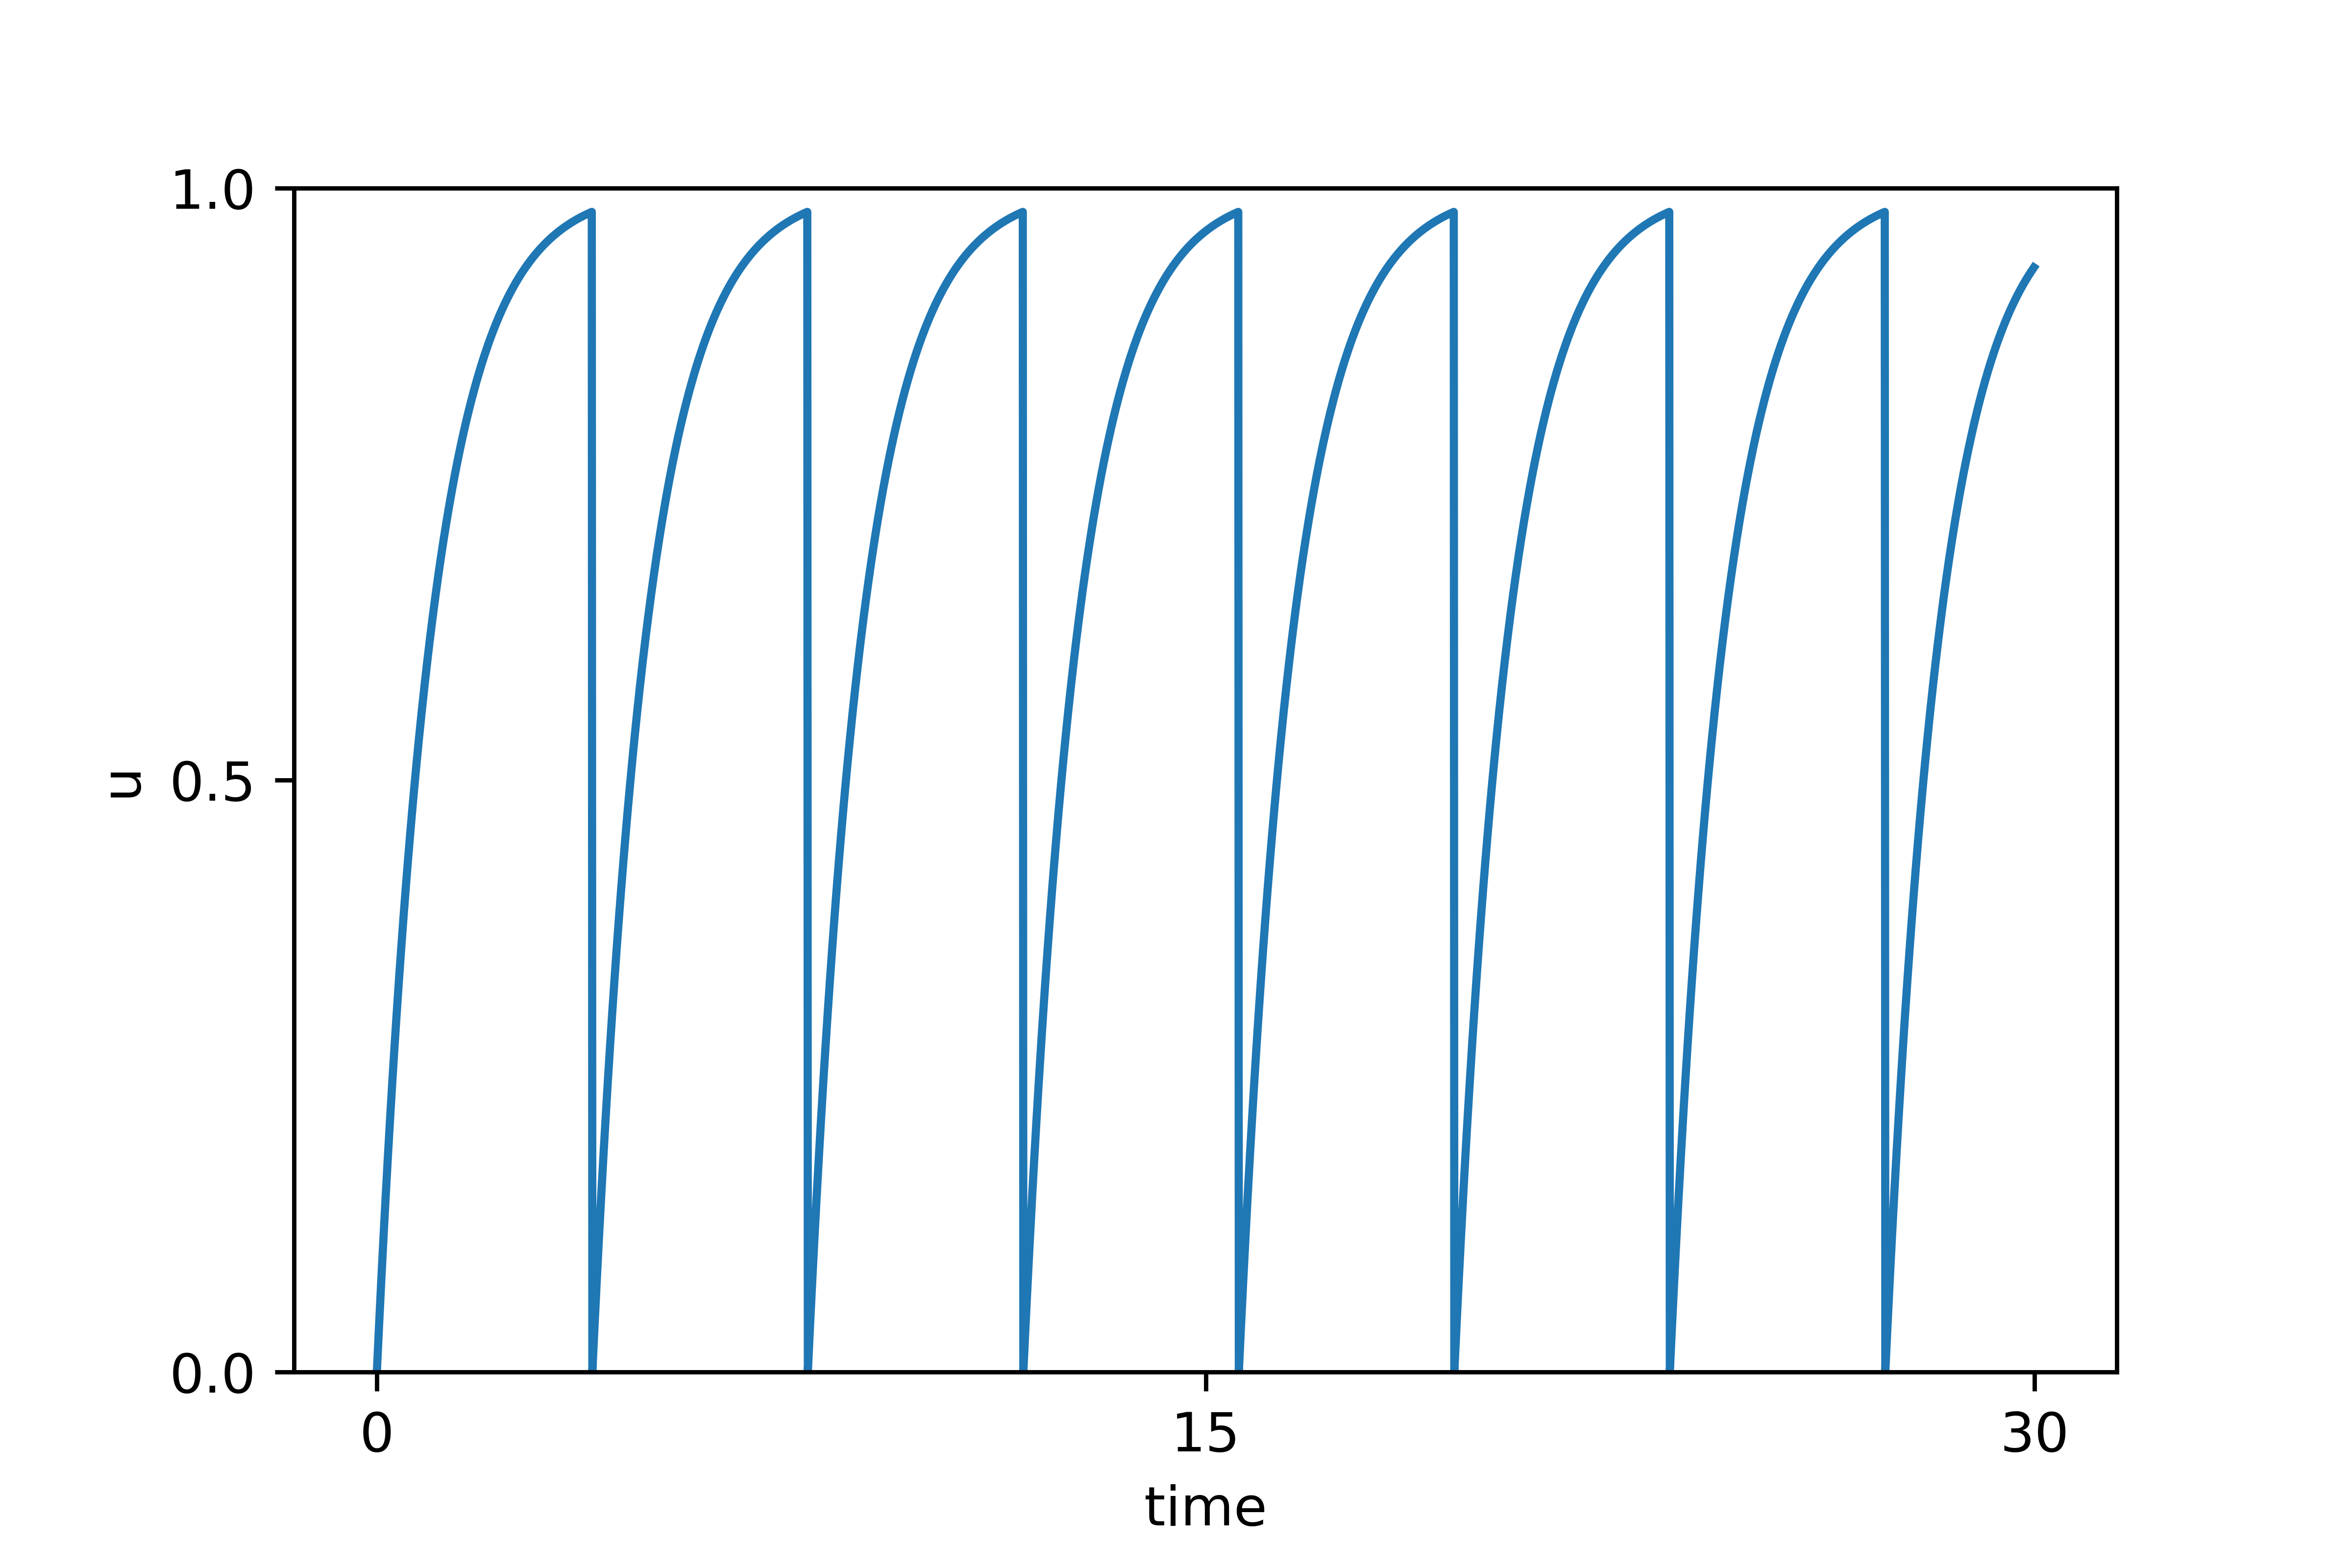
\includegraphics[width=0.8 \textwidth]{lif_single.png}
\caption{Dynamic evolution of the membrane potential in time according to Eq. (\ref{eq1}) and (\ref{eq2}).}
\end{figure}
\end{frame}

\subsection{Nonlocally coupled network of LIF neurons}
\begin{frame}{Nonlocally coupled network of LIF neurons} \pause
  \begin{itemize}
  \item $N$ LIF neurons that are arranged in a regular ring topology \pause
  \item non-local connections: each element is coupled to its $R$ nearest neighbours on either side \pause
  \item dynamical evolution
  \begin{equation} \label{eqncon}
\frac{d u_i(t)}{dt} = \mu - \lambda \, u_i + \frac{\sigma}{2 R} \sum_{j=i-R}^{j=i+R} [u_i(t) - u_j(t)],
\end{equation} \pause
\item index $i$ taken modulo $N$ 
  \end{itemize}
\end{frame}

\section{Methods}
\begin{frame}{Methods} \pause
\begin{itemize}
\item conventional PC \pause
\item coded in Python \pause
\item total processing time $\approx 240$ hours \pause
\item code verified by reproducing some of the results in the bibliography \pause
\item forward Euler method, step size of $dt = 0.01$

\end{itemize}
\end{frame}

\section{Chimera states in coupled LIF neurons}
\subsection{Minimum number of neurons and $\Delta \omega$ vs $N$}
\begin{frame}{Minimum number of neurons} \pause

\begin{figure}[H]
\begin{subfigure}{.32\textwidth}
  \centering
  % include first image
  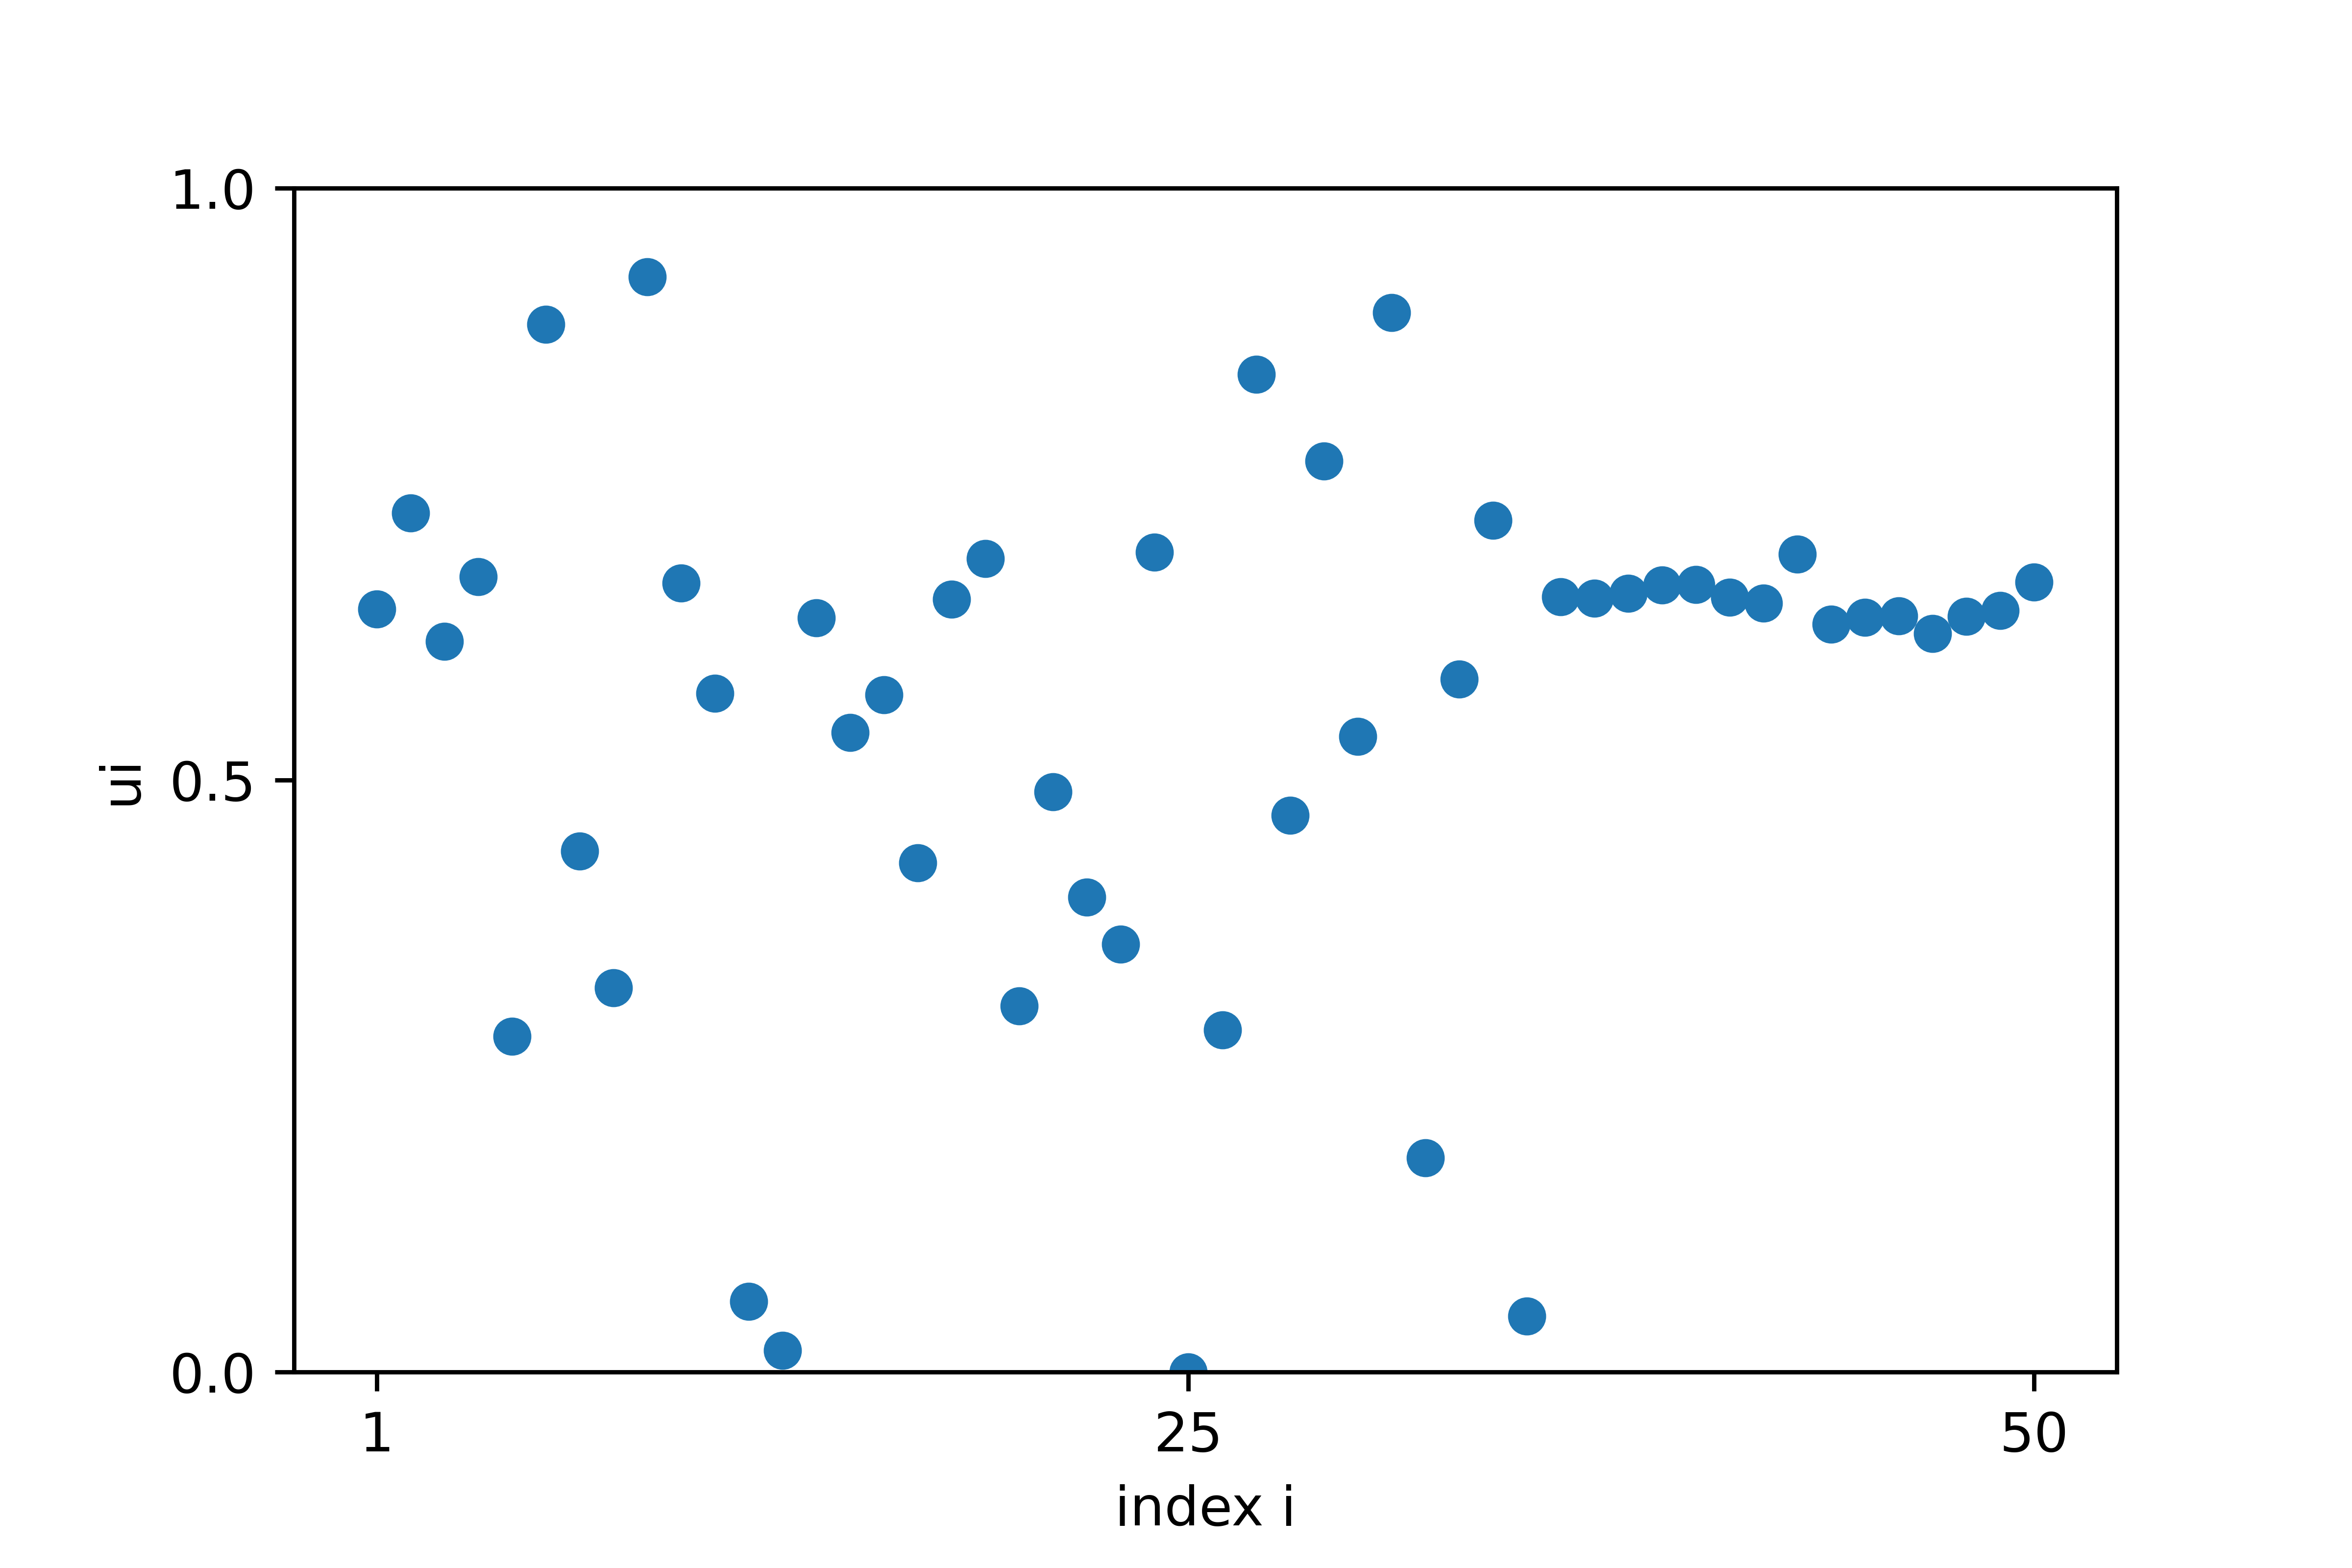
\includegraphics[width=1\linewidth]{u_N=50.png}  
  \caption{$N=50$}
\end{subfigure}
\hfill
\begin{subfigure}{.32\textwidth}
  \centering
  % include second image
  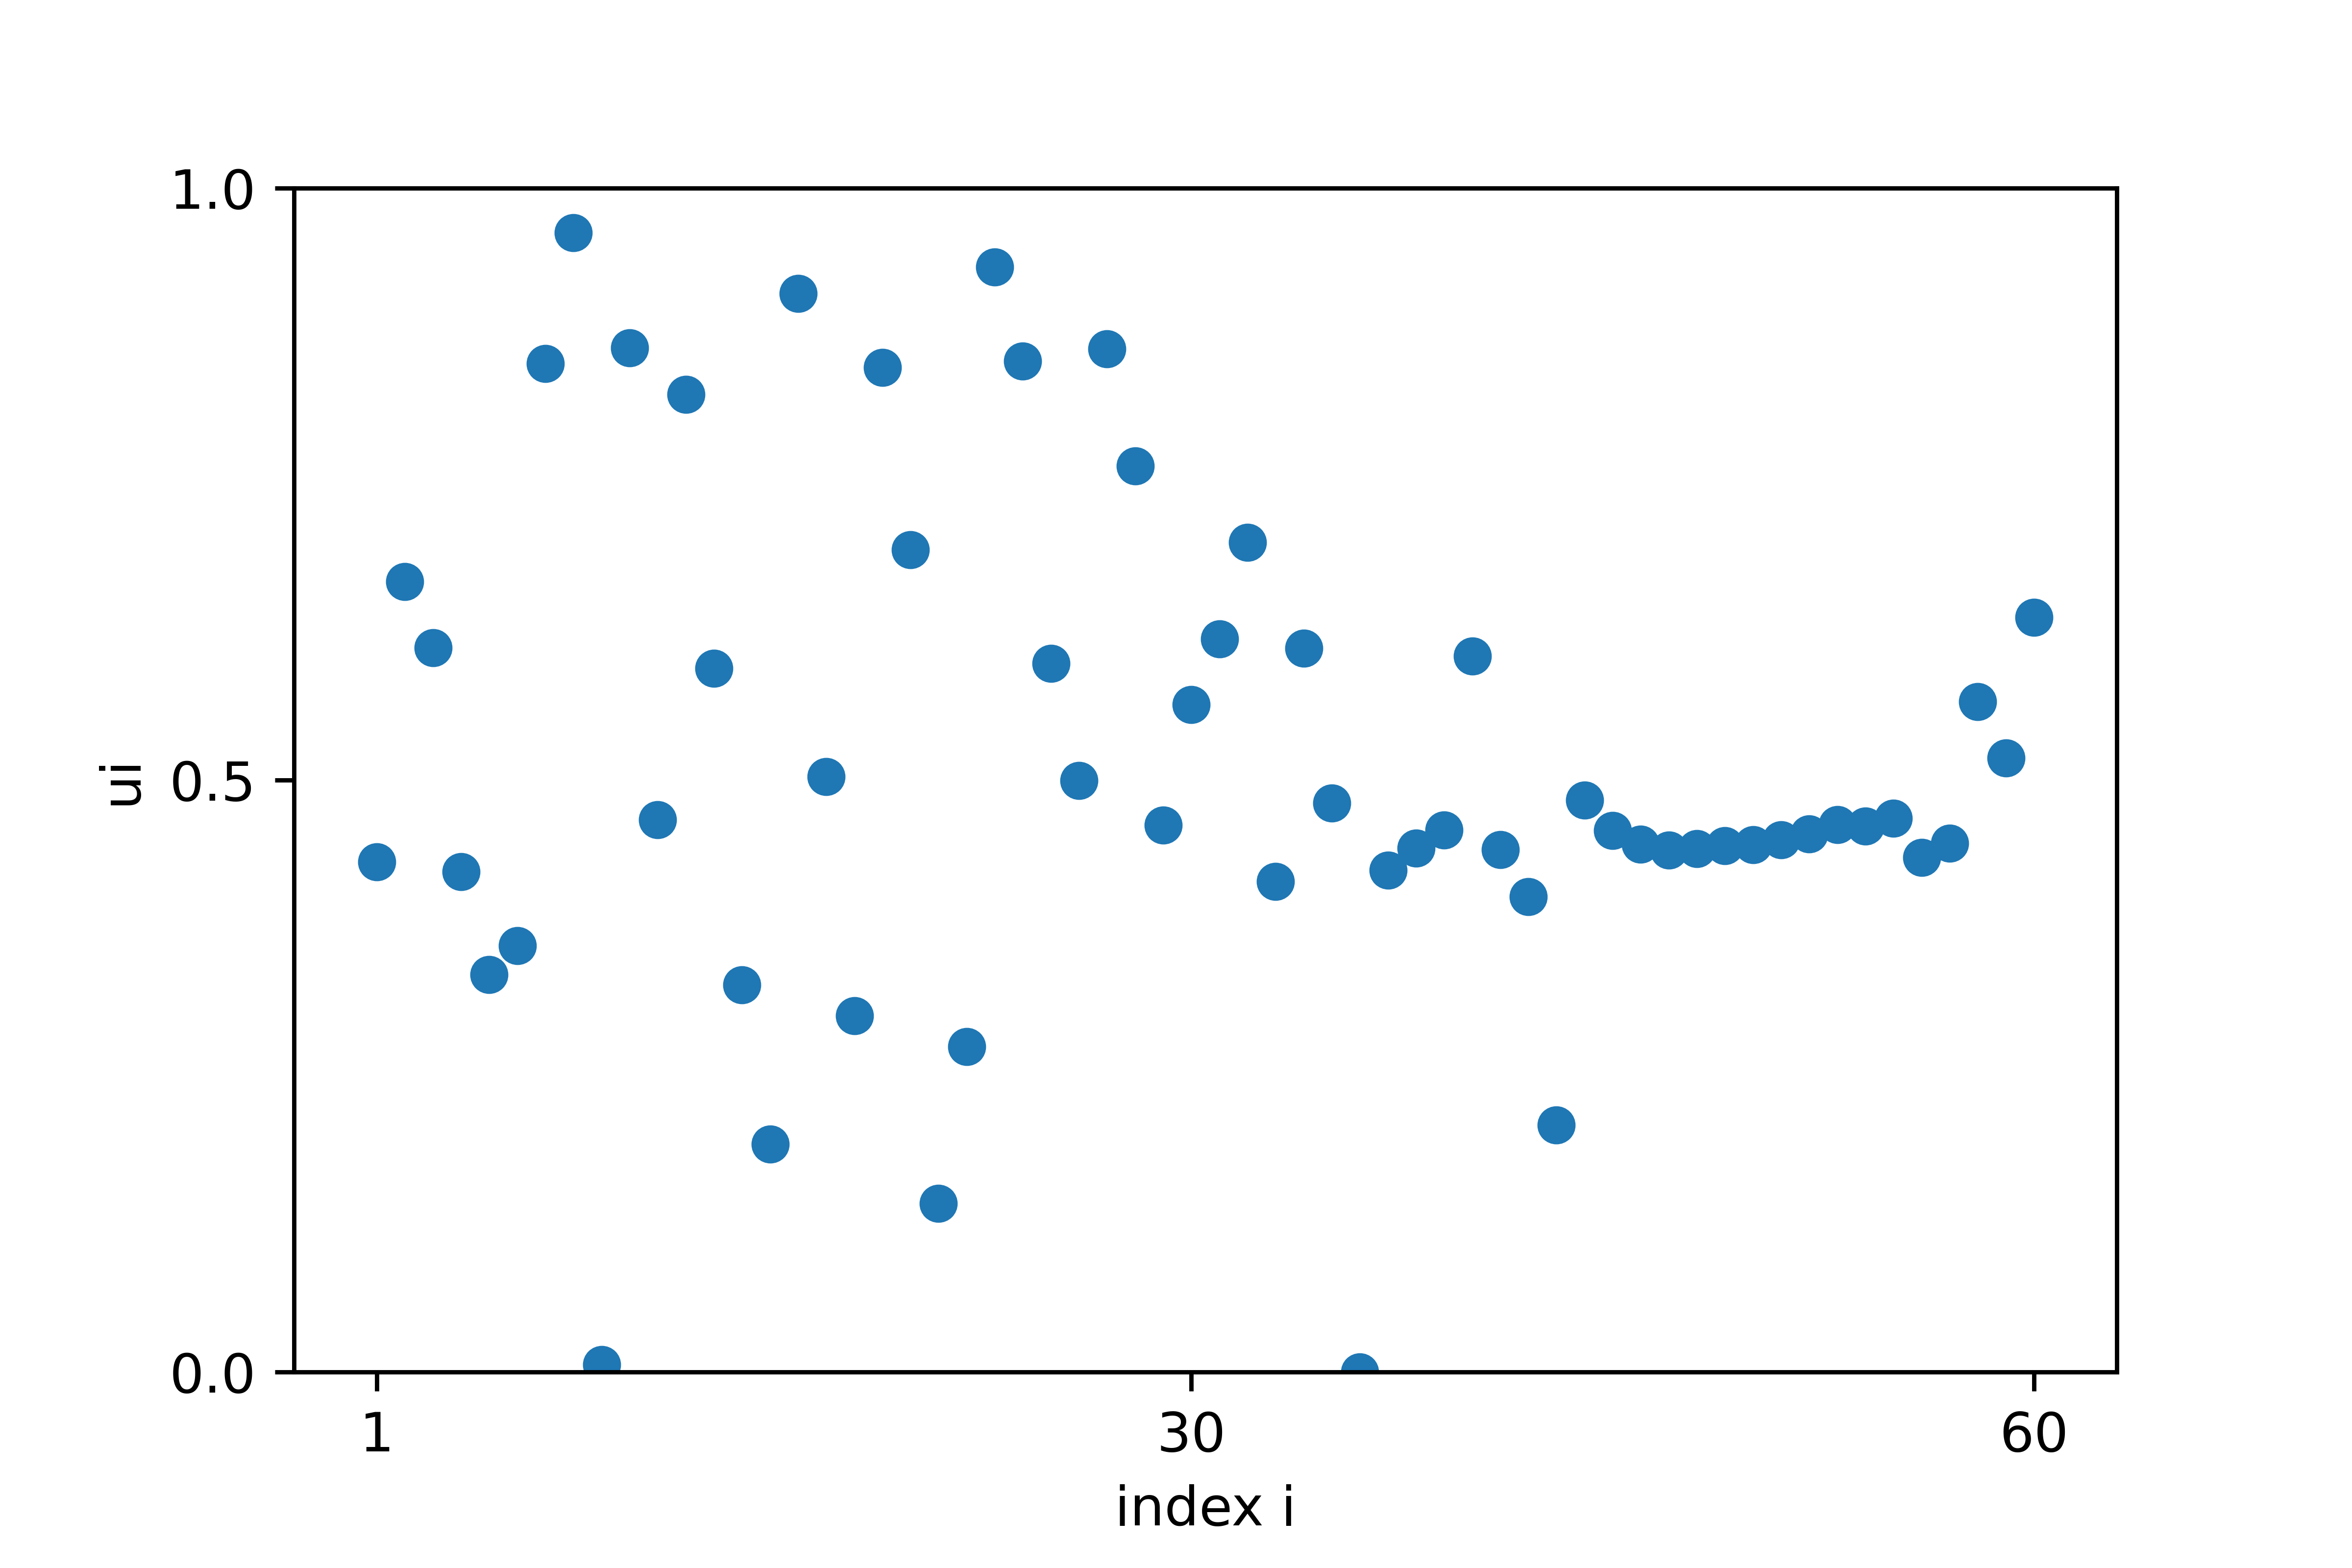
\includegraphics[width=1\linewidth]{u_N=60.png}  
  \caption{$N=60$}
\end{subfigure}
\hfill
\begin{subfigure}{.32\textwidth}
  \centering
  % include first image
  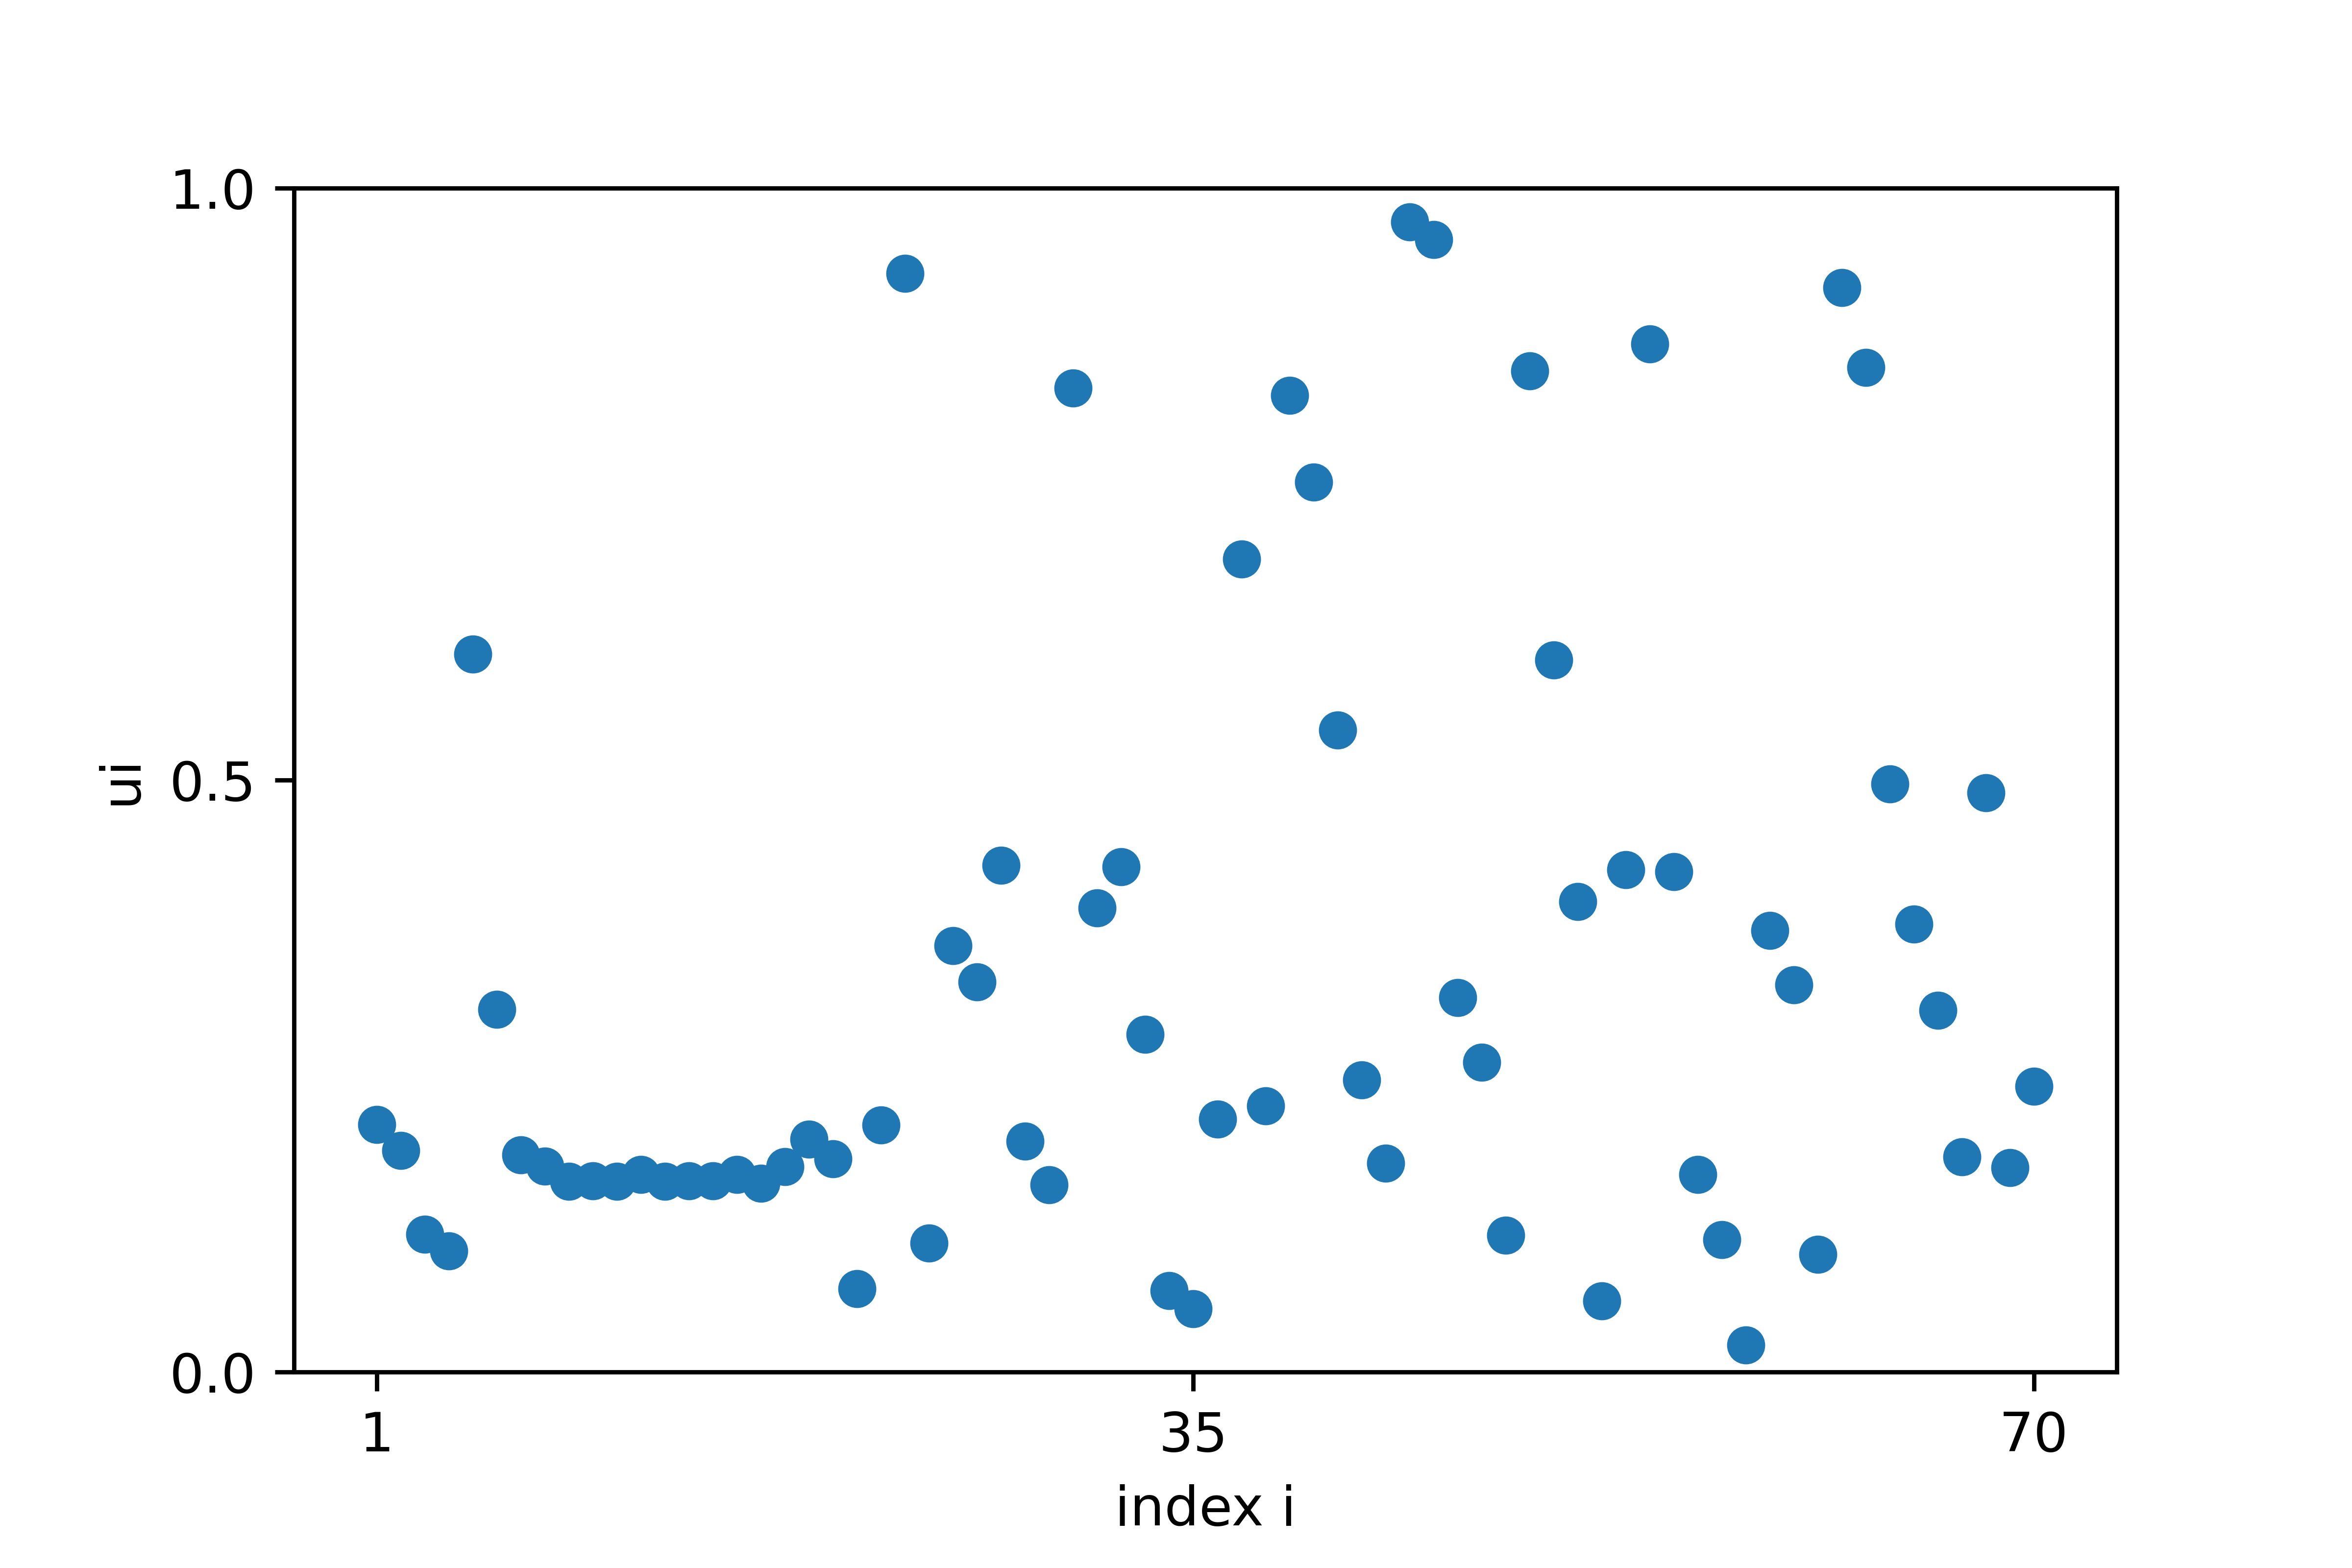
\includegraphics[width=1\linewidth]{u_N=70.png}  
  \caption{$N=70$}
\end{subfigure}
\begin{subfigure}{.32\textwidth}
  \centering
  % include first image
  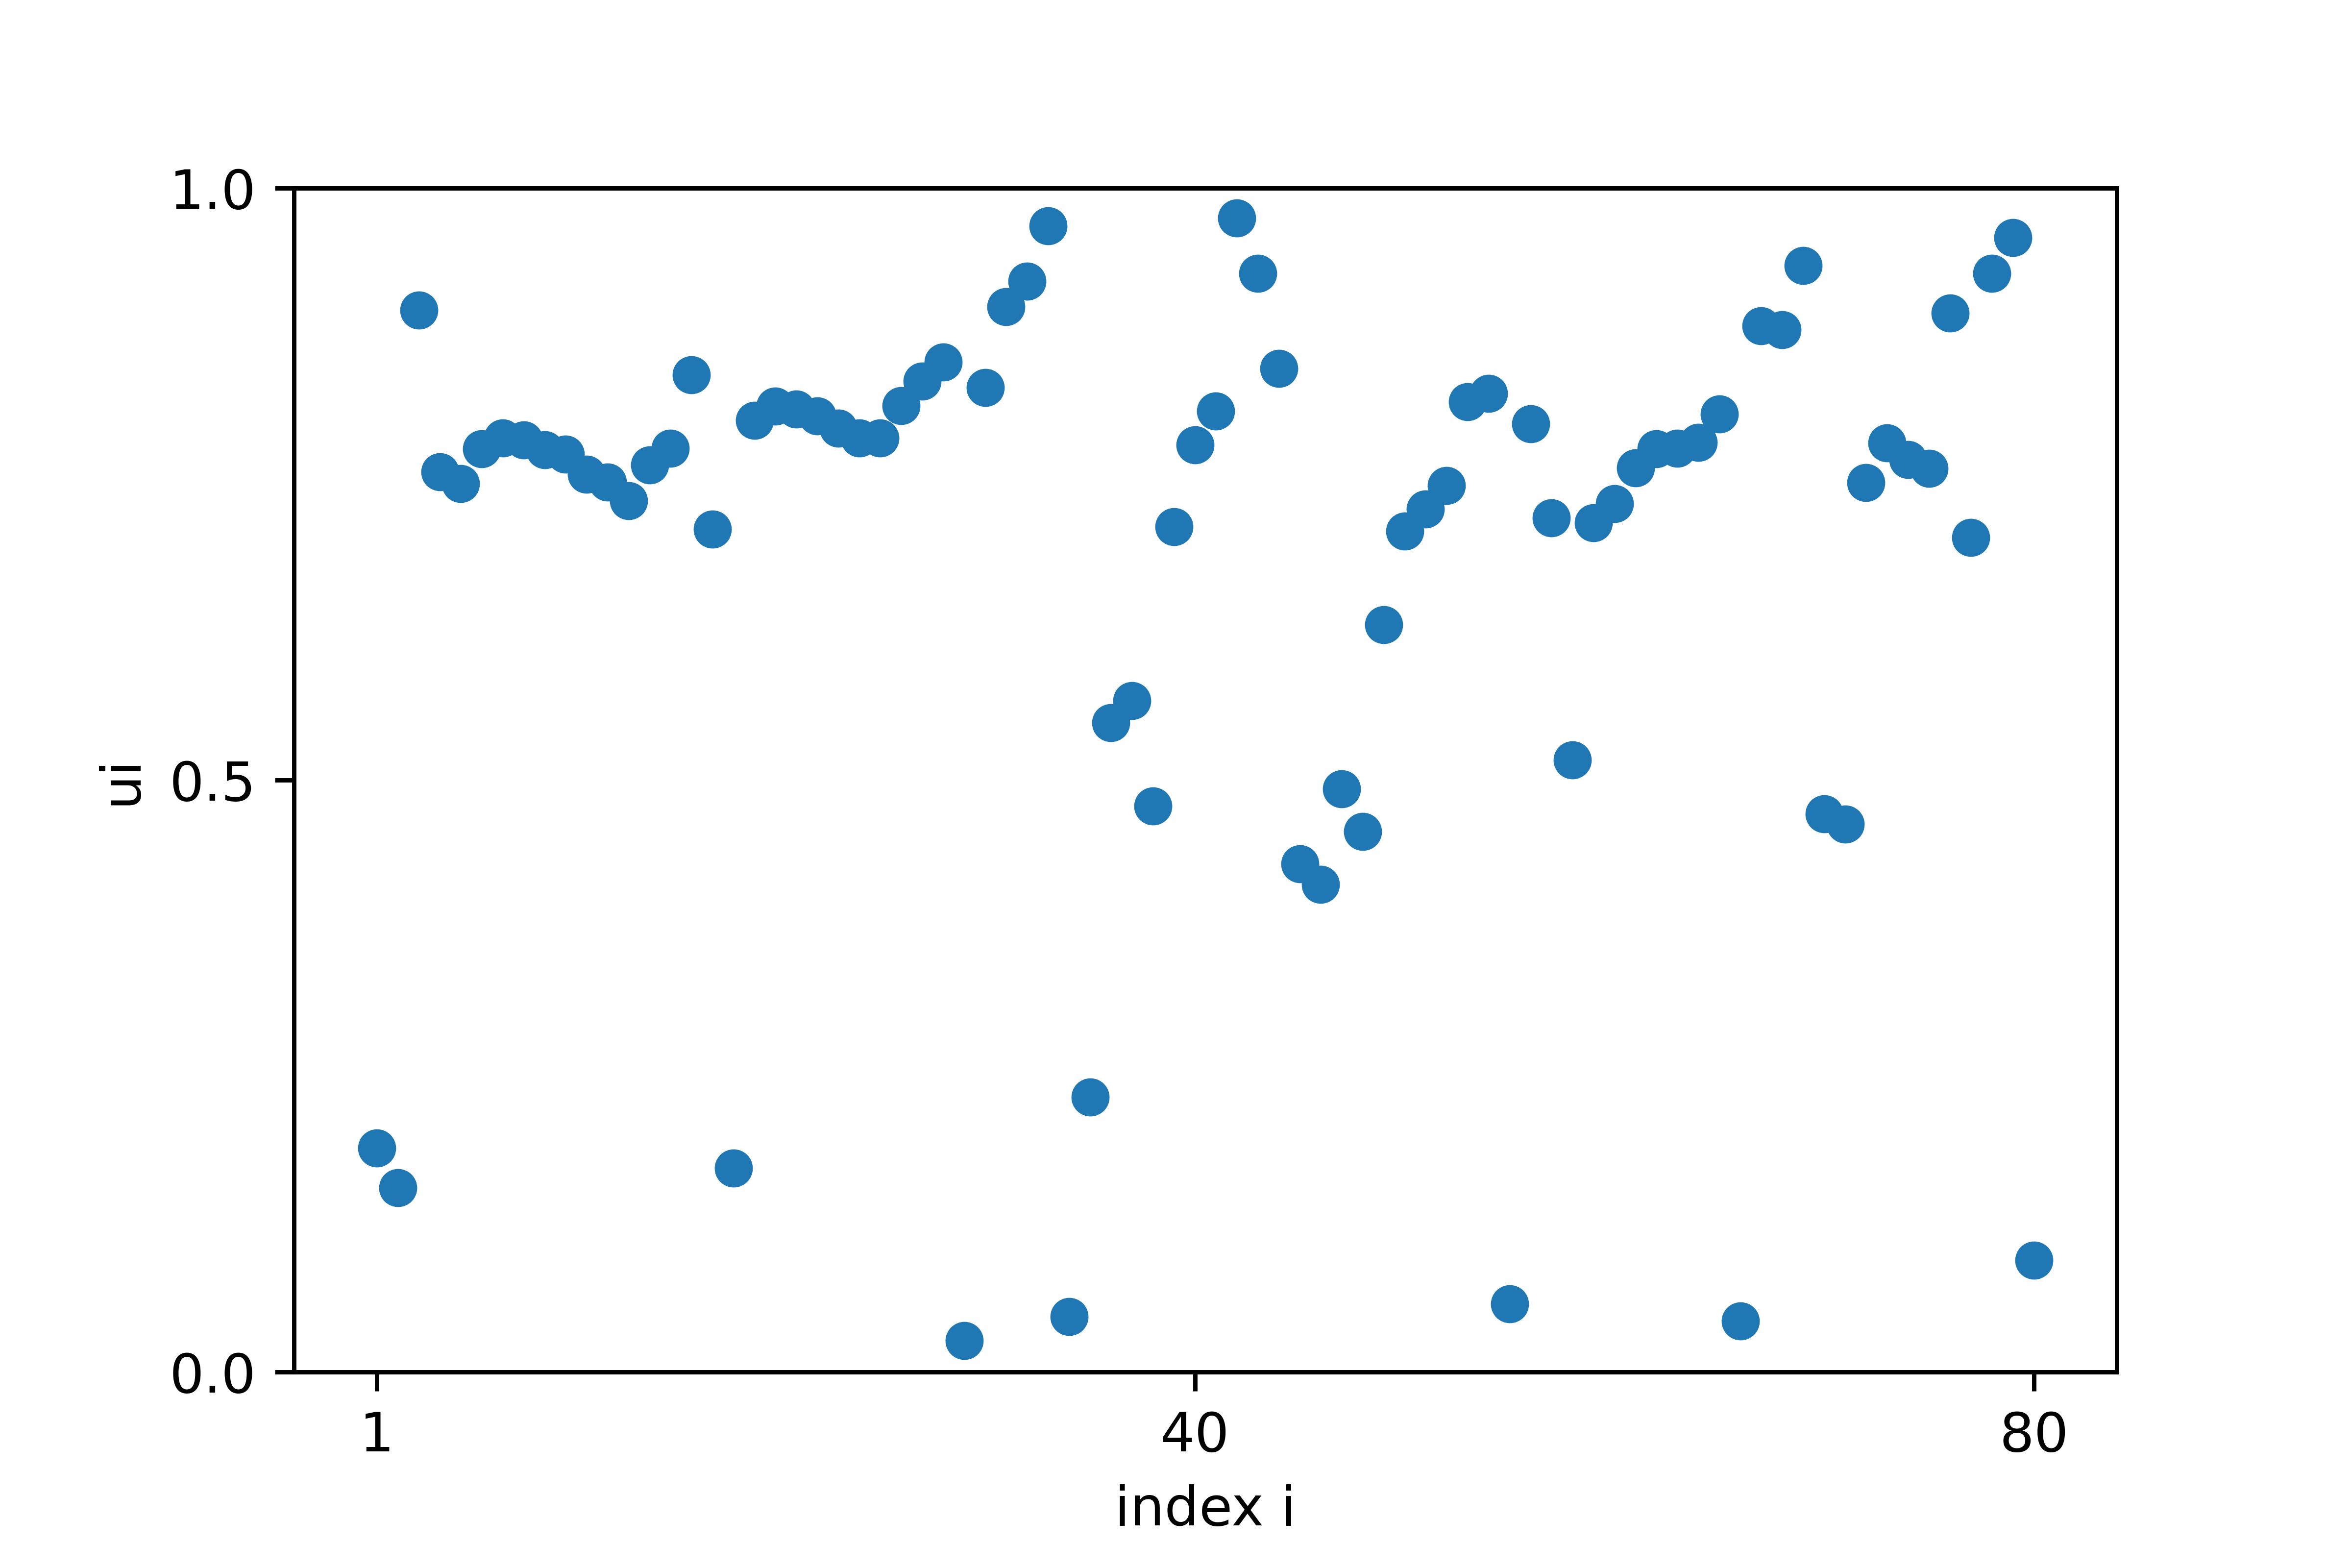
\includegraphics[width=1\linewidth]{u_N=80.png}  
  \caption{$N=80$}
\end{subfigure}
\hfill
\begin{subfigure}{.32\textwidth}
  \centering
  % include first image
  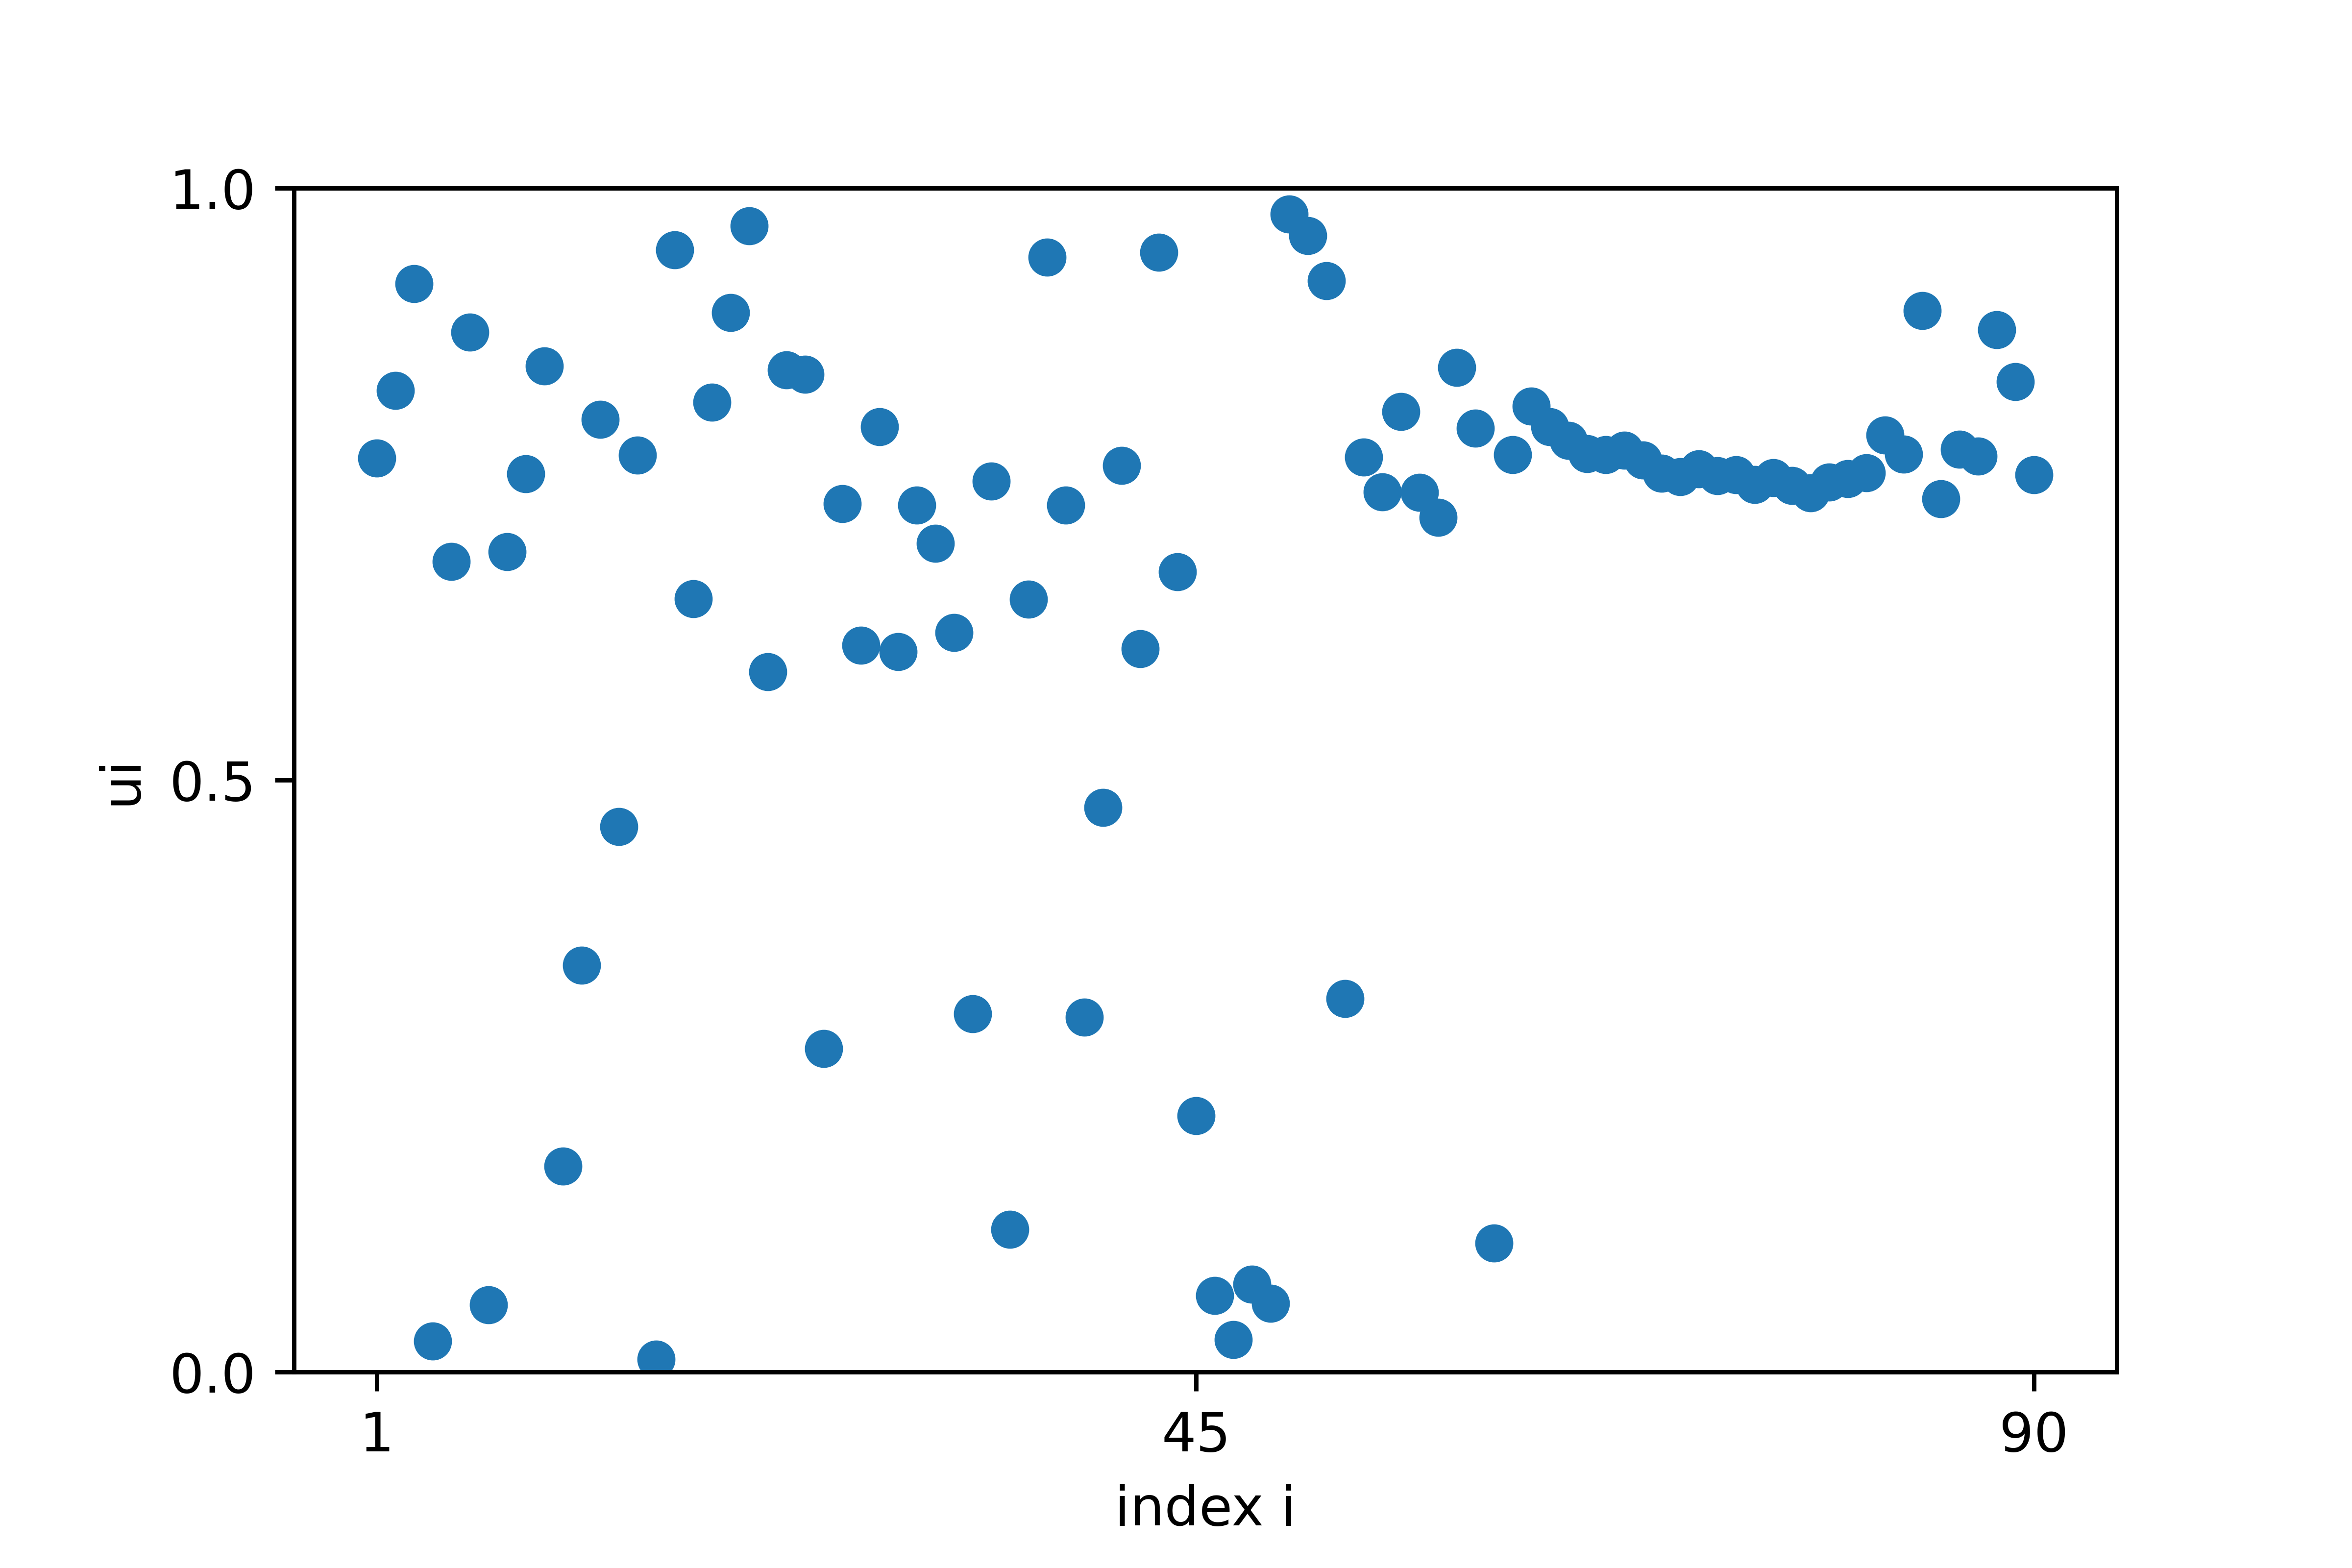
\includegraphics[width=1\linewidth]{u_N=90.png}  
  \caption{$N=90$}
\end{subfigure}
\hfill
\begin{subfigure}{.32\textwidth}
  \centering
  % include first image
  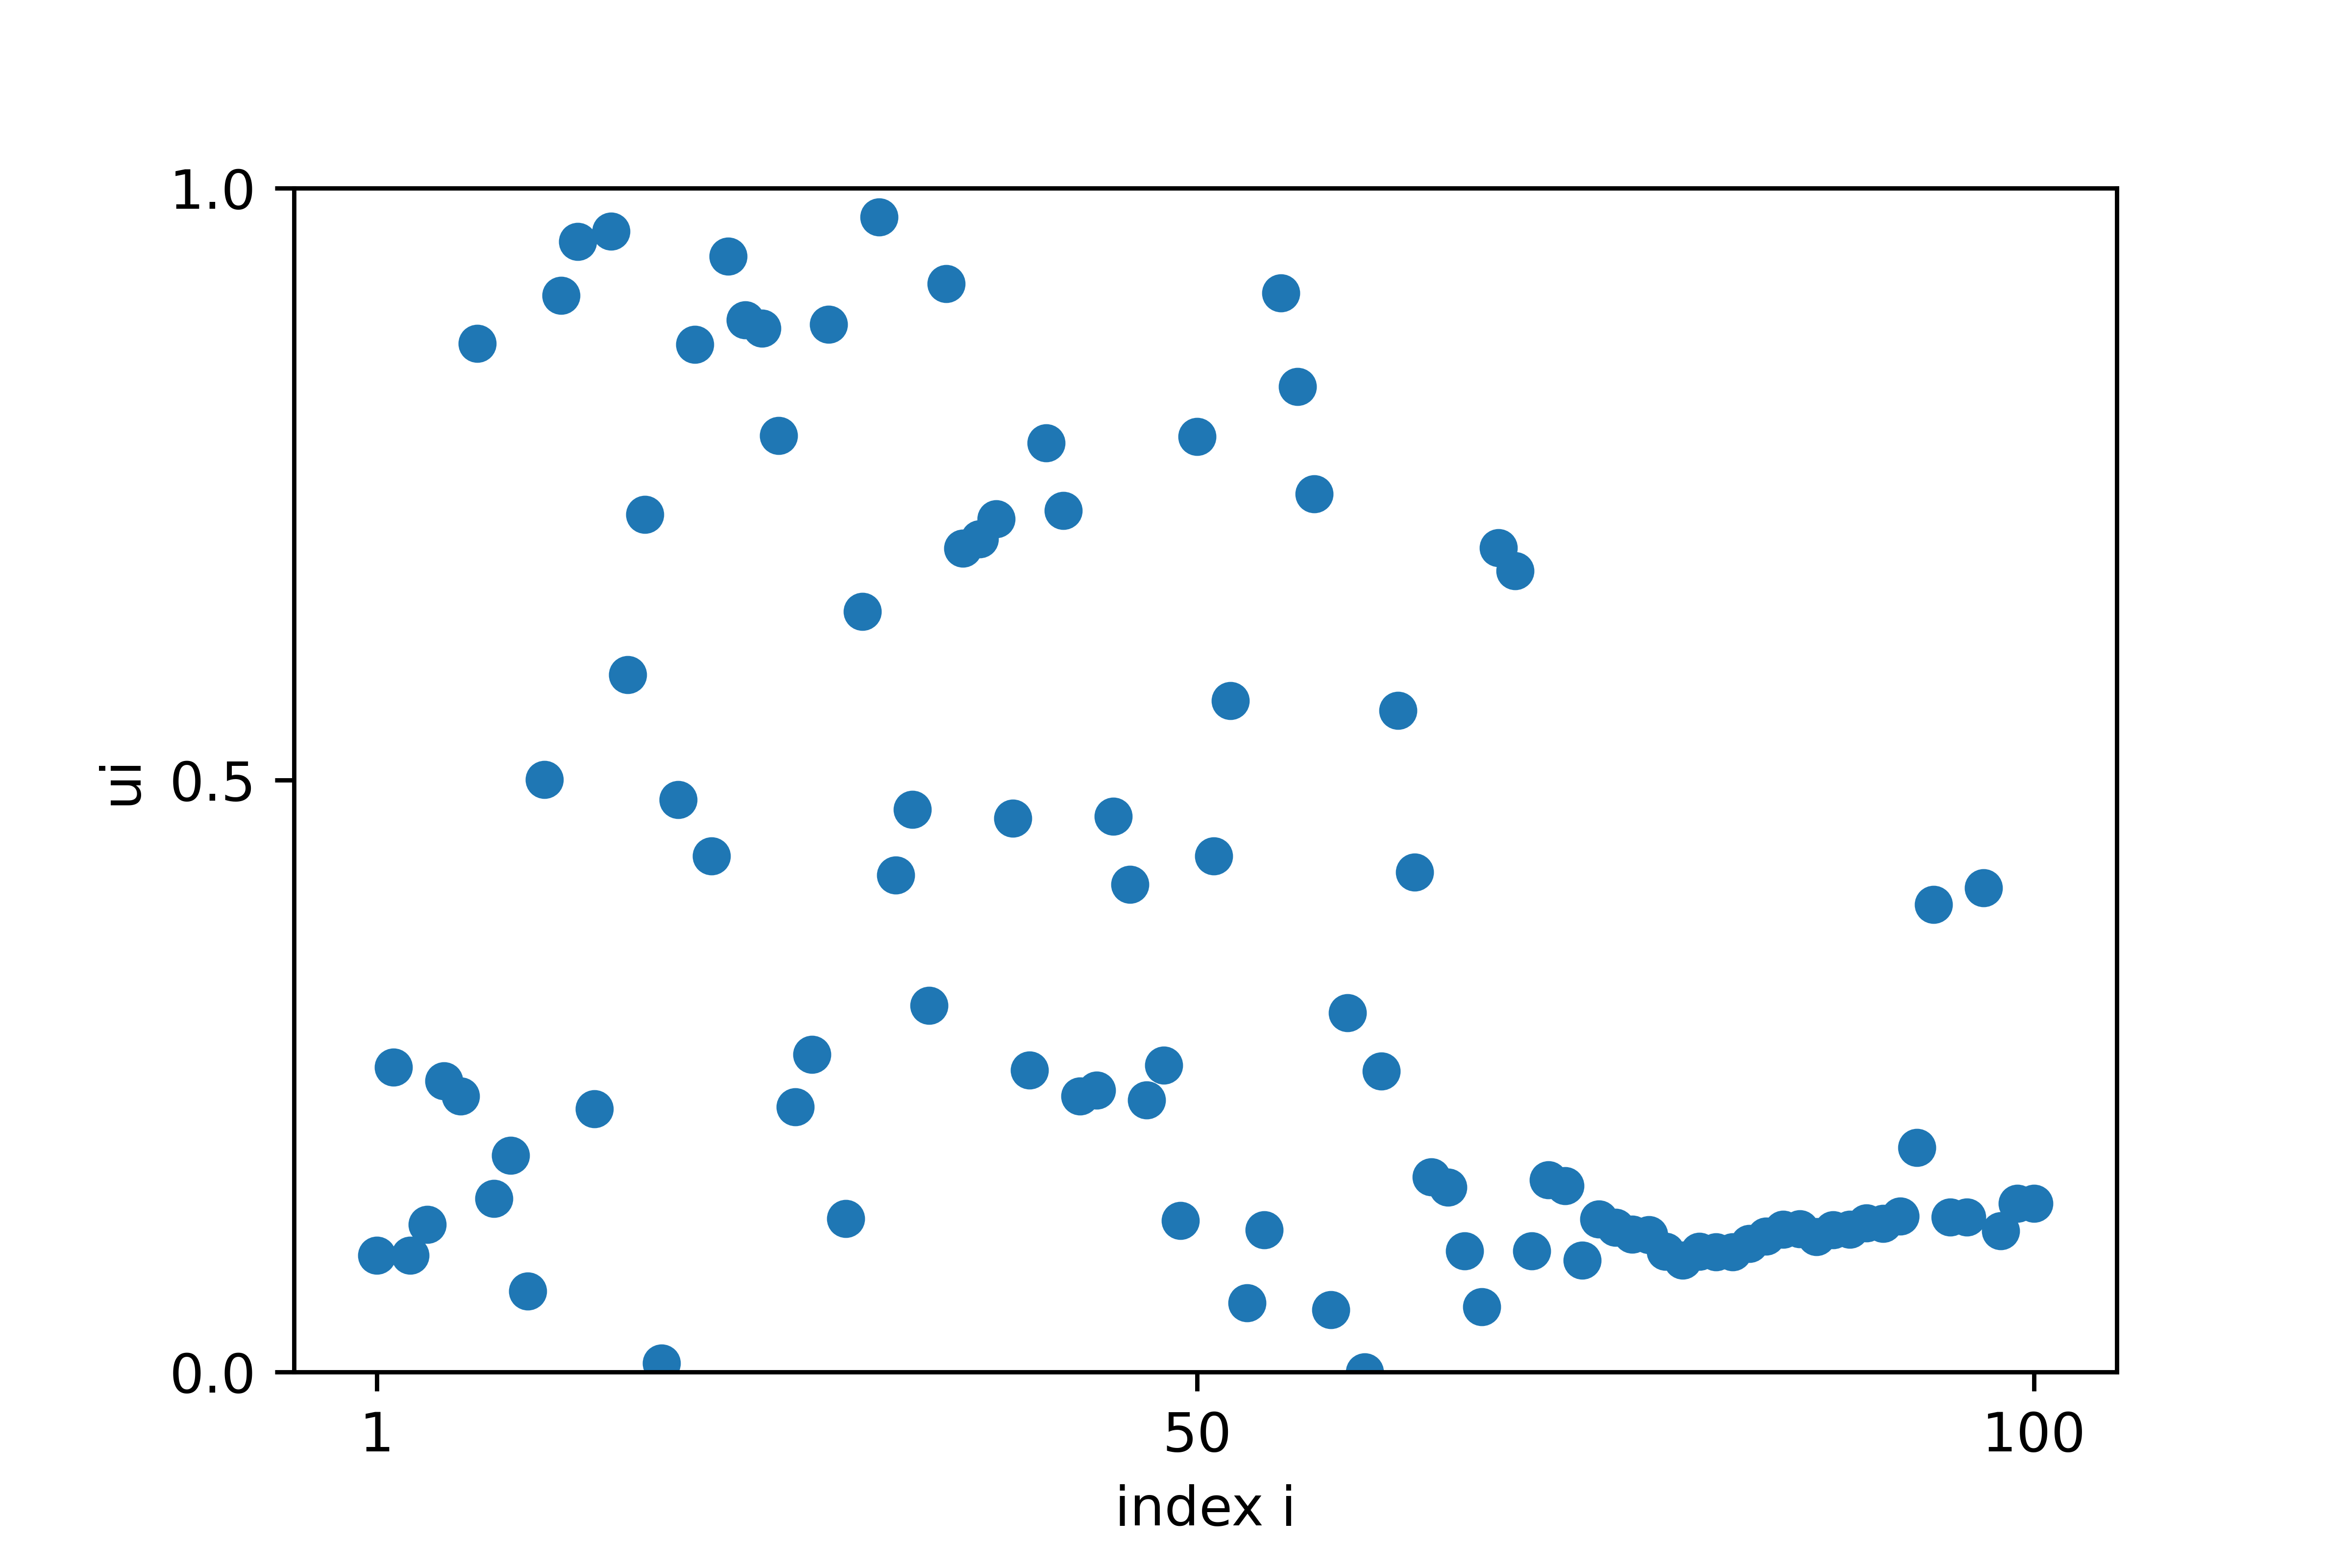
\includegraphics[width=1\linewidth]{u_N=100.png}  
  \caption{$N=100$}
\end{subfigure}
\caption{Snapshots of the membrane potential $u_i$ at $t=1000$ time units, for $\sigma = 0.7$, $r=0.40$ and for various values of $N$.}
\label{vsN}
\end{figure}
\end{frame}

\begin{frame}{Minimum number of neurons}
\begin{figure}[H]
\begin{subfigure}{.32\textwidth}
  \centering
  % include first image
  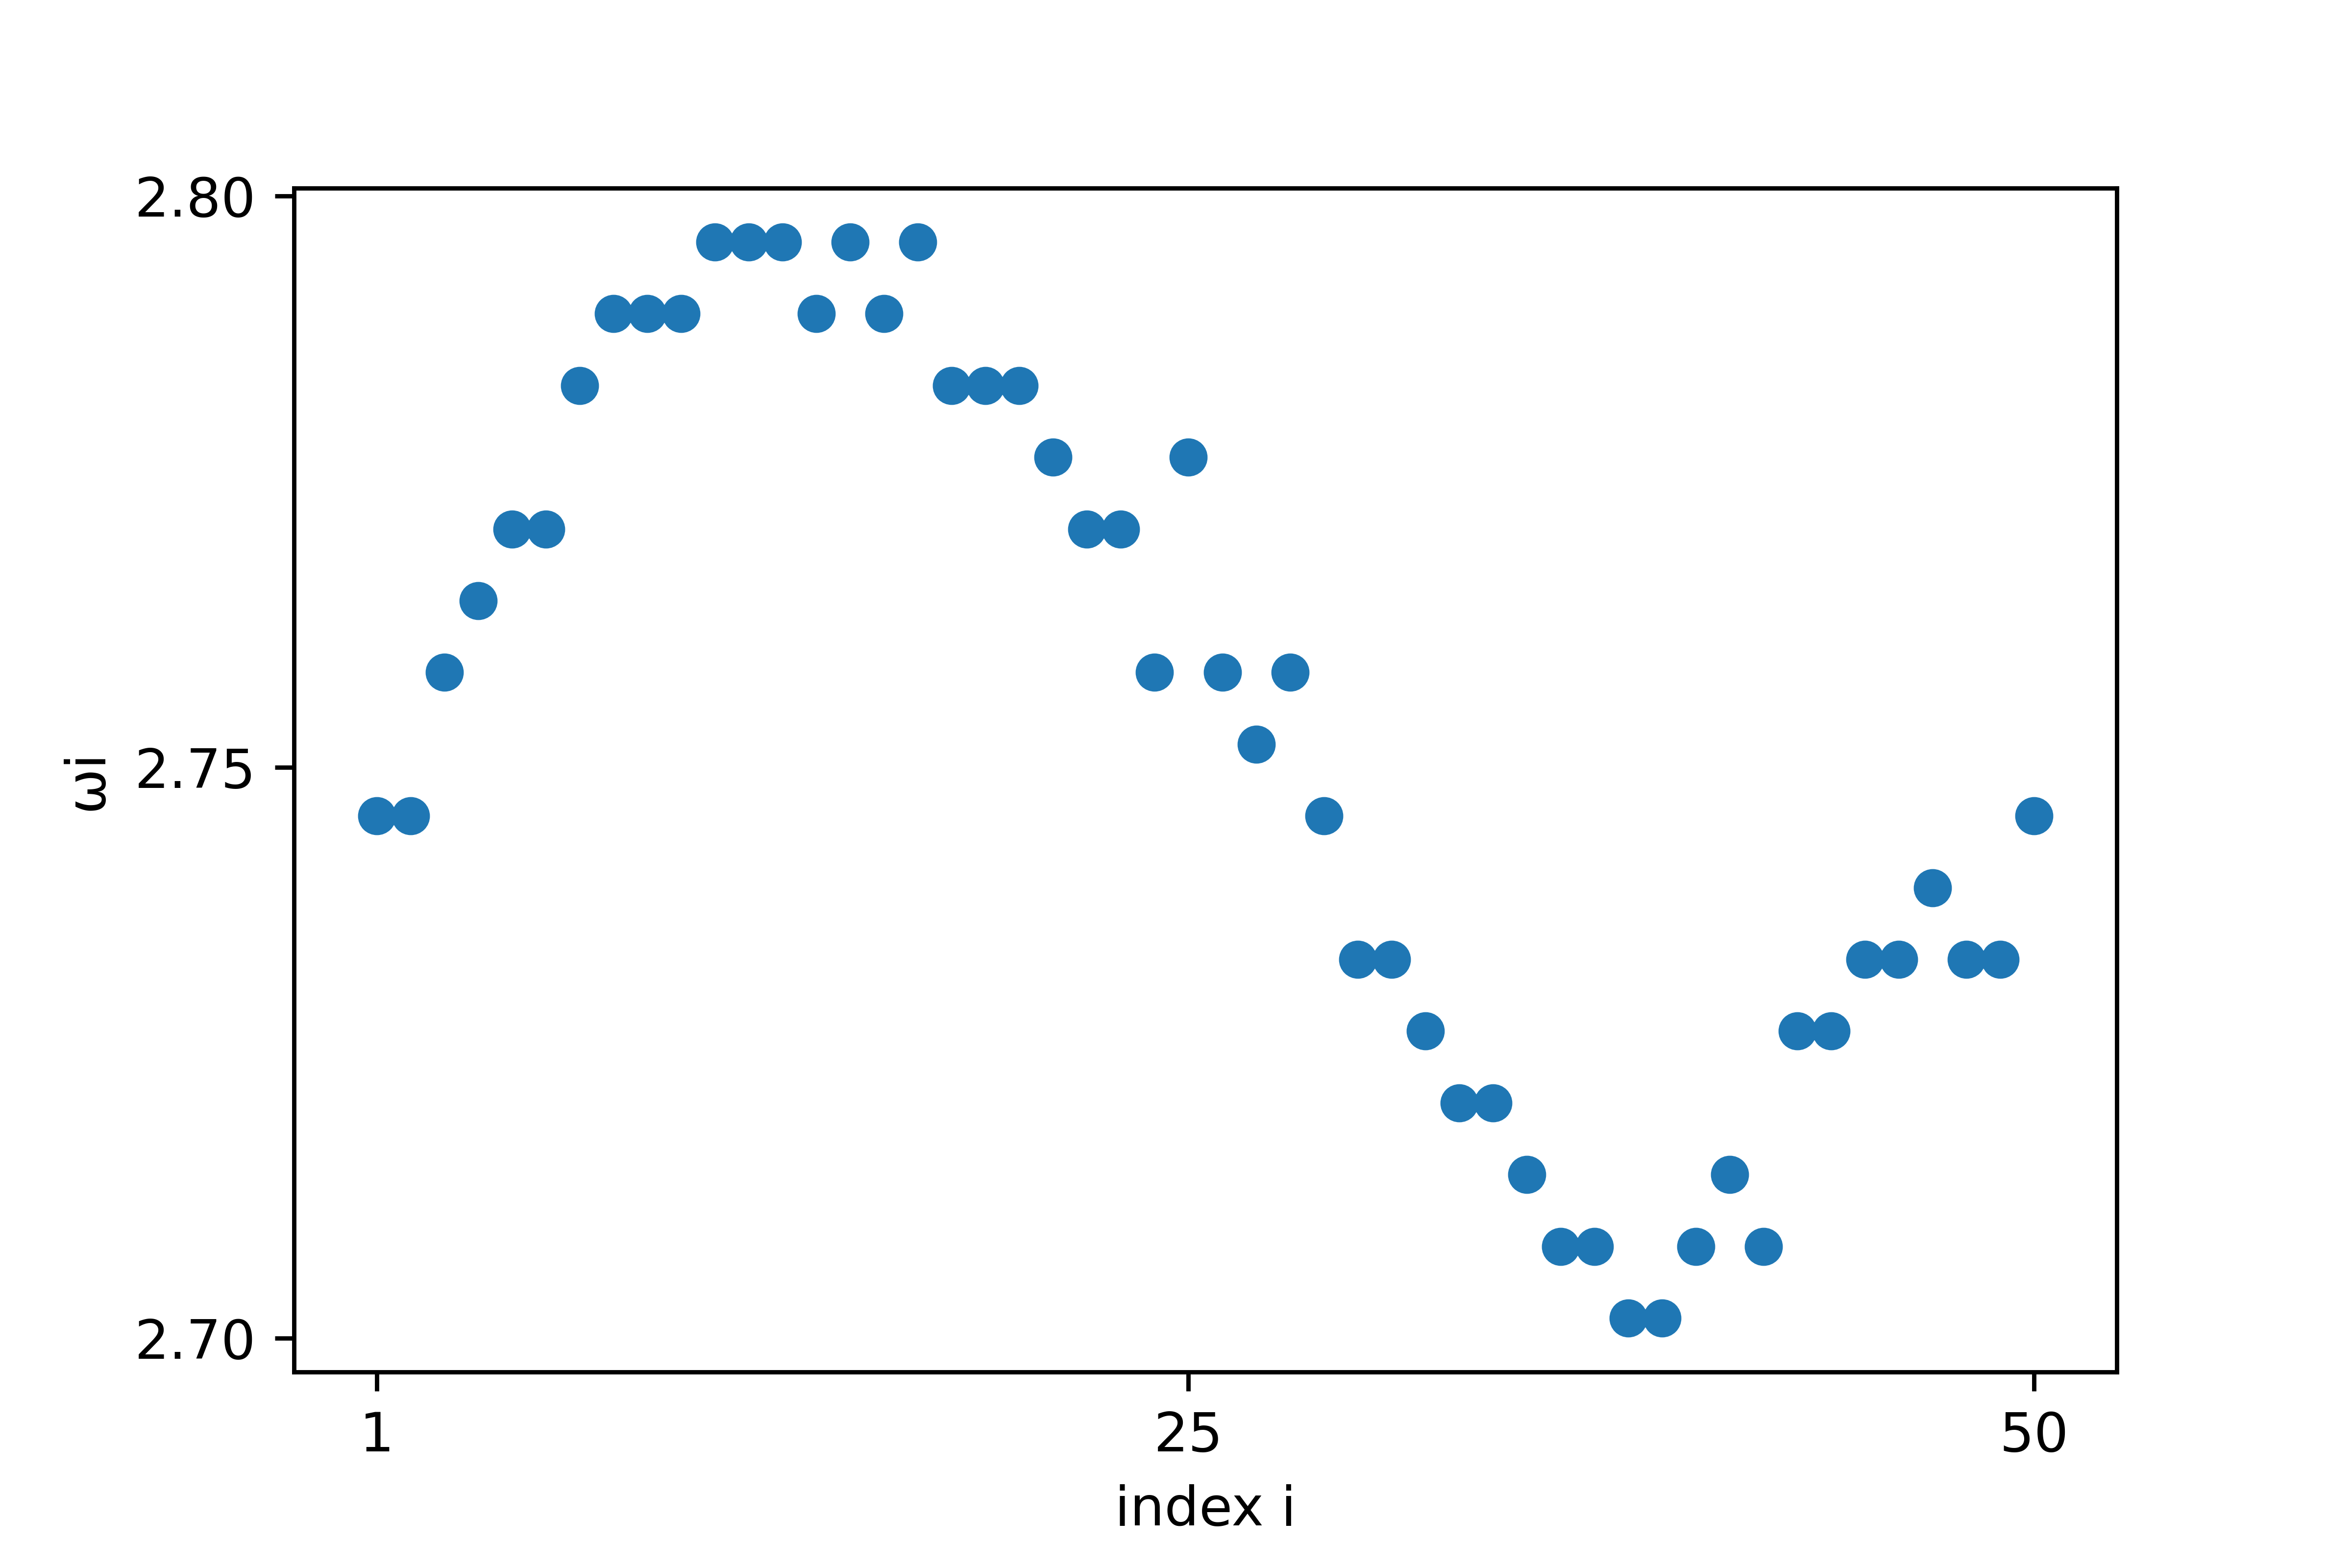
\includegraphics[width=1\linewidth]{w_N=50.png}  
  \caption{$N=50$}
\end{subfigure}
\hfill
\begin{subfigure}{.32\textwidth}
  \centering
  % include second image
  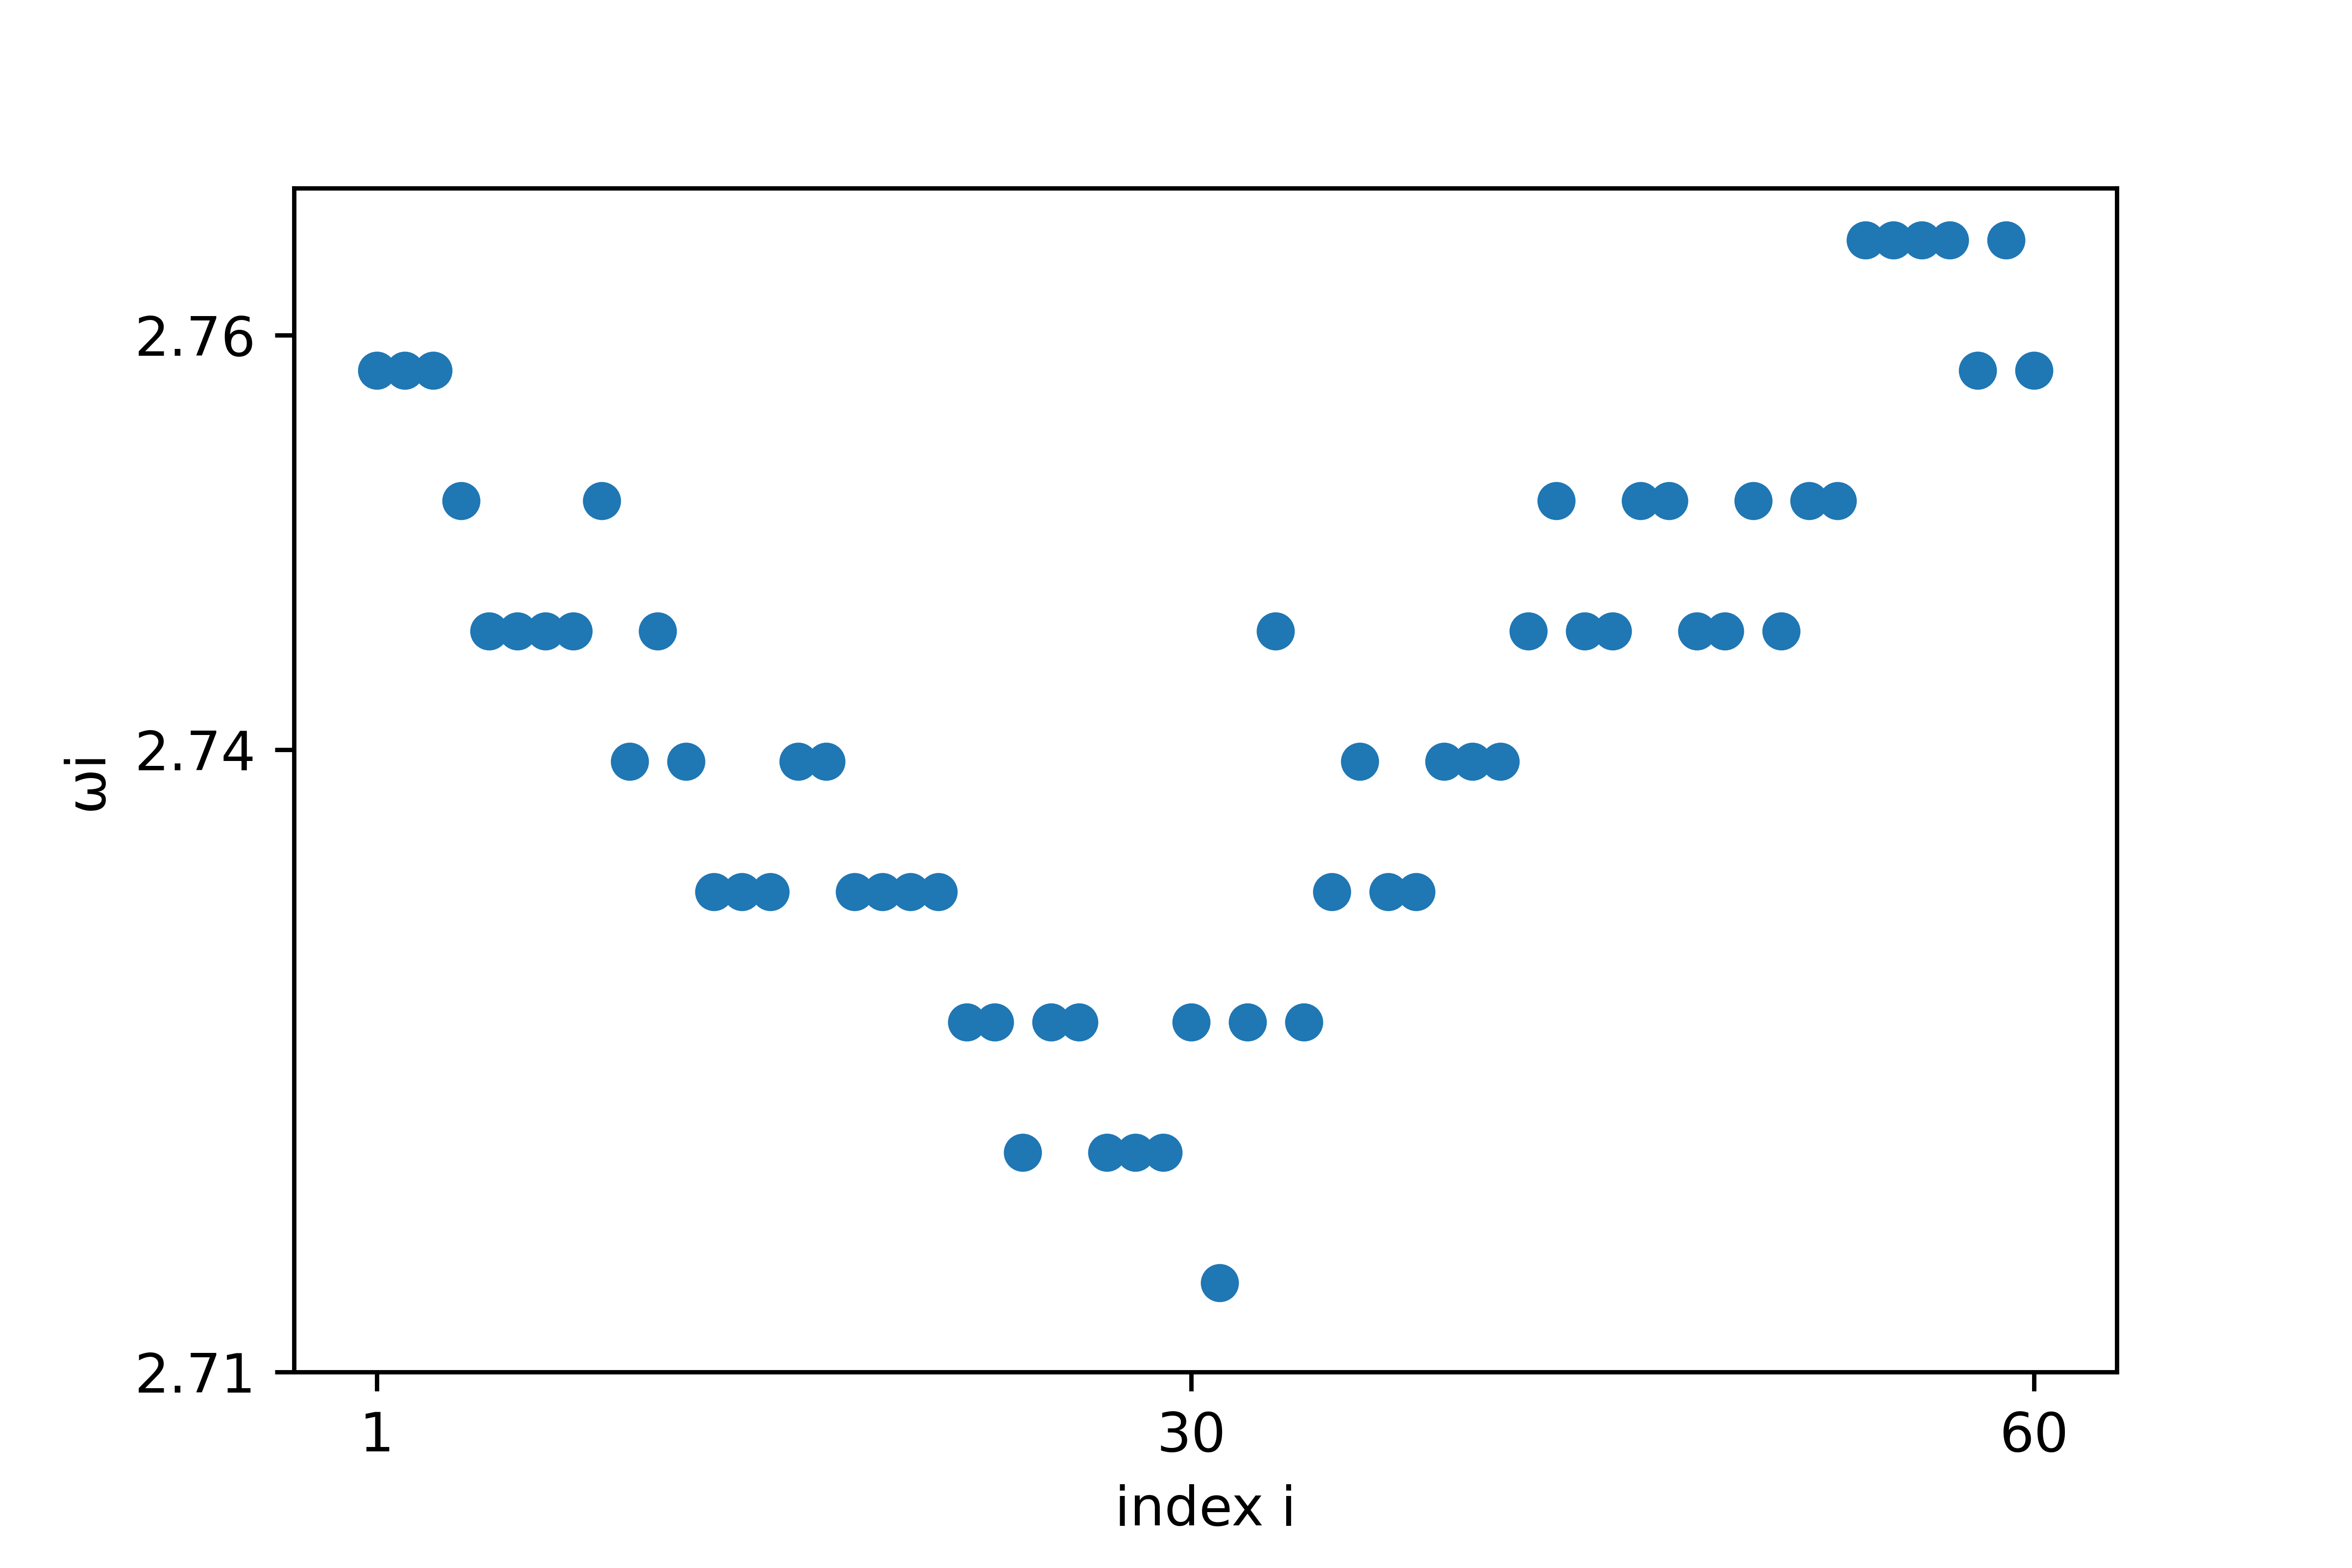
\includegraphics[width=1\linewidth]{w_N=60.png}  
  \caption{$N=60$}
\end{subfigure}
\hfill
\begin{subfigure}{.32\textwidth}
  \centering
  % include first image
  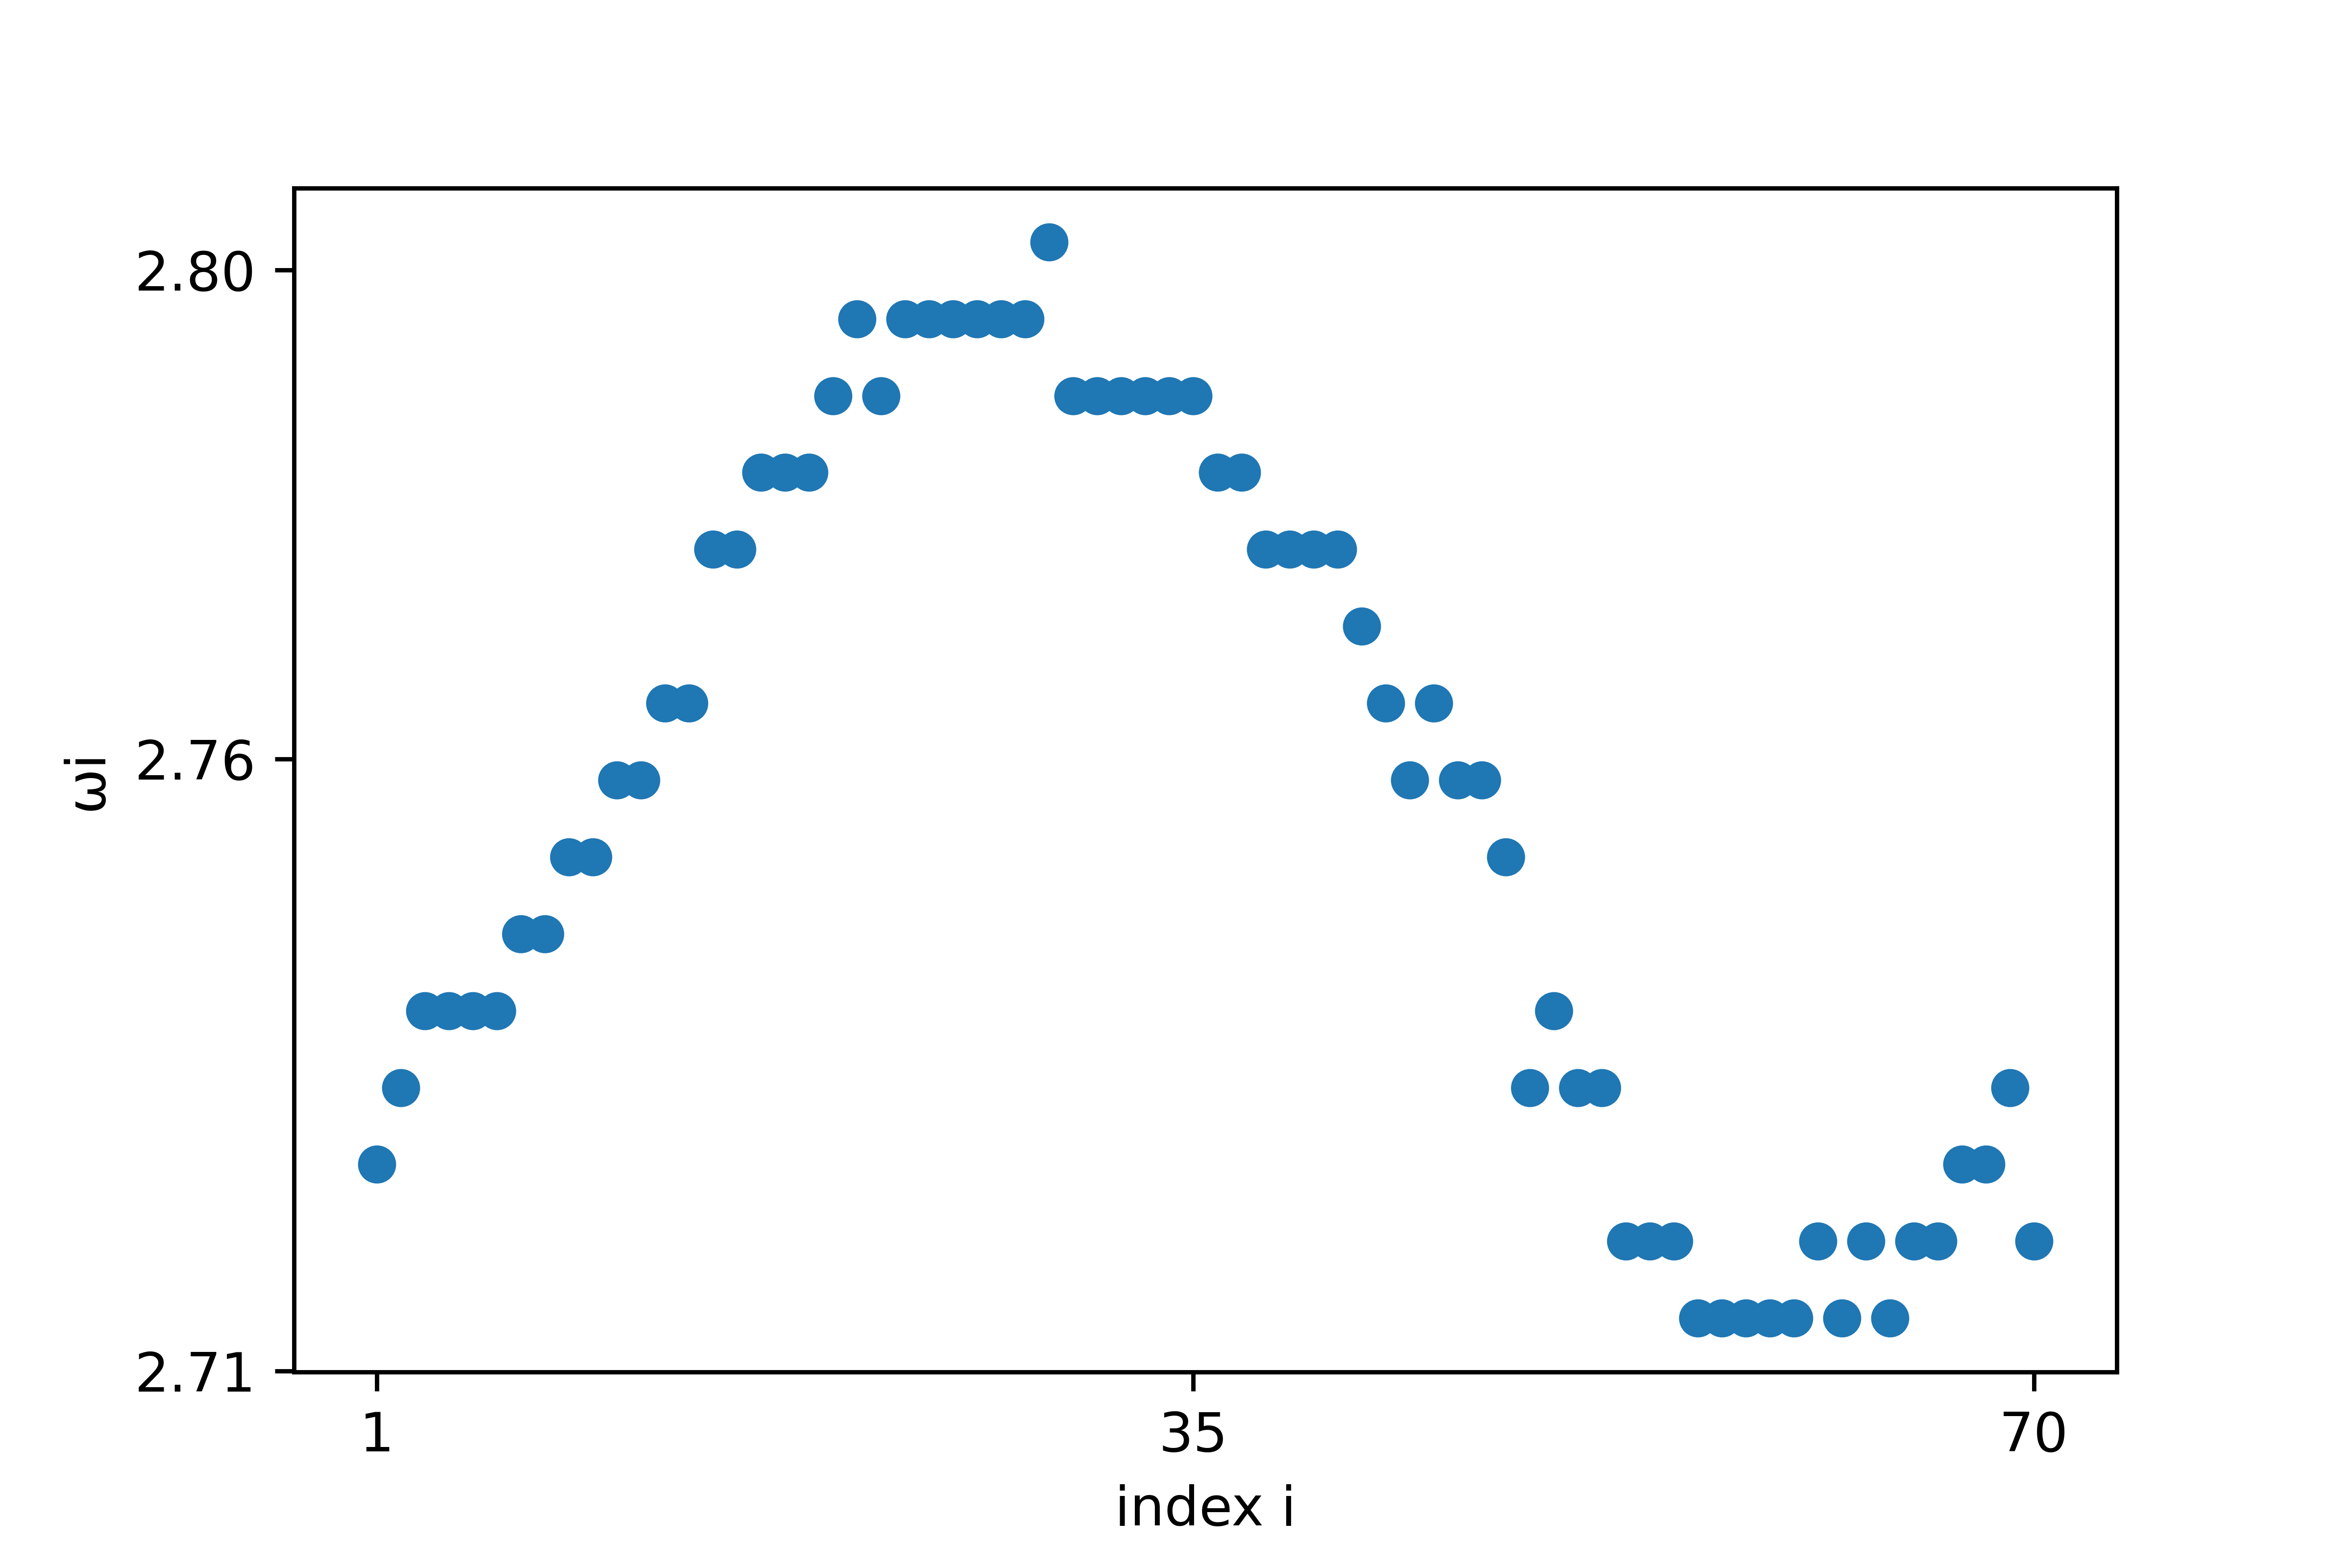
\includegraphics[width=1\linewidth]{w_N=70.png}  
  \caption{$N=70$}
\end{subfigure}
\begin{subfigure}{.32\textwidth}
  \centering
  % include first image
  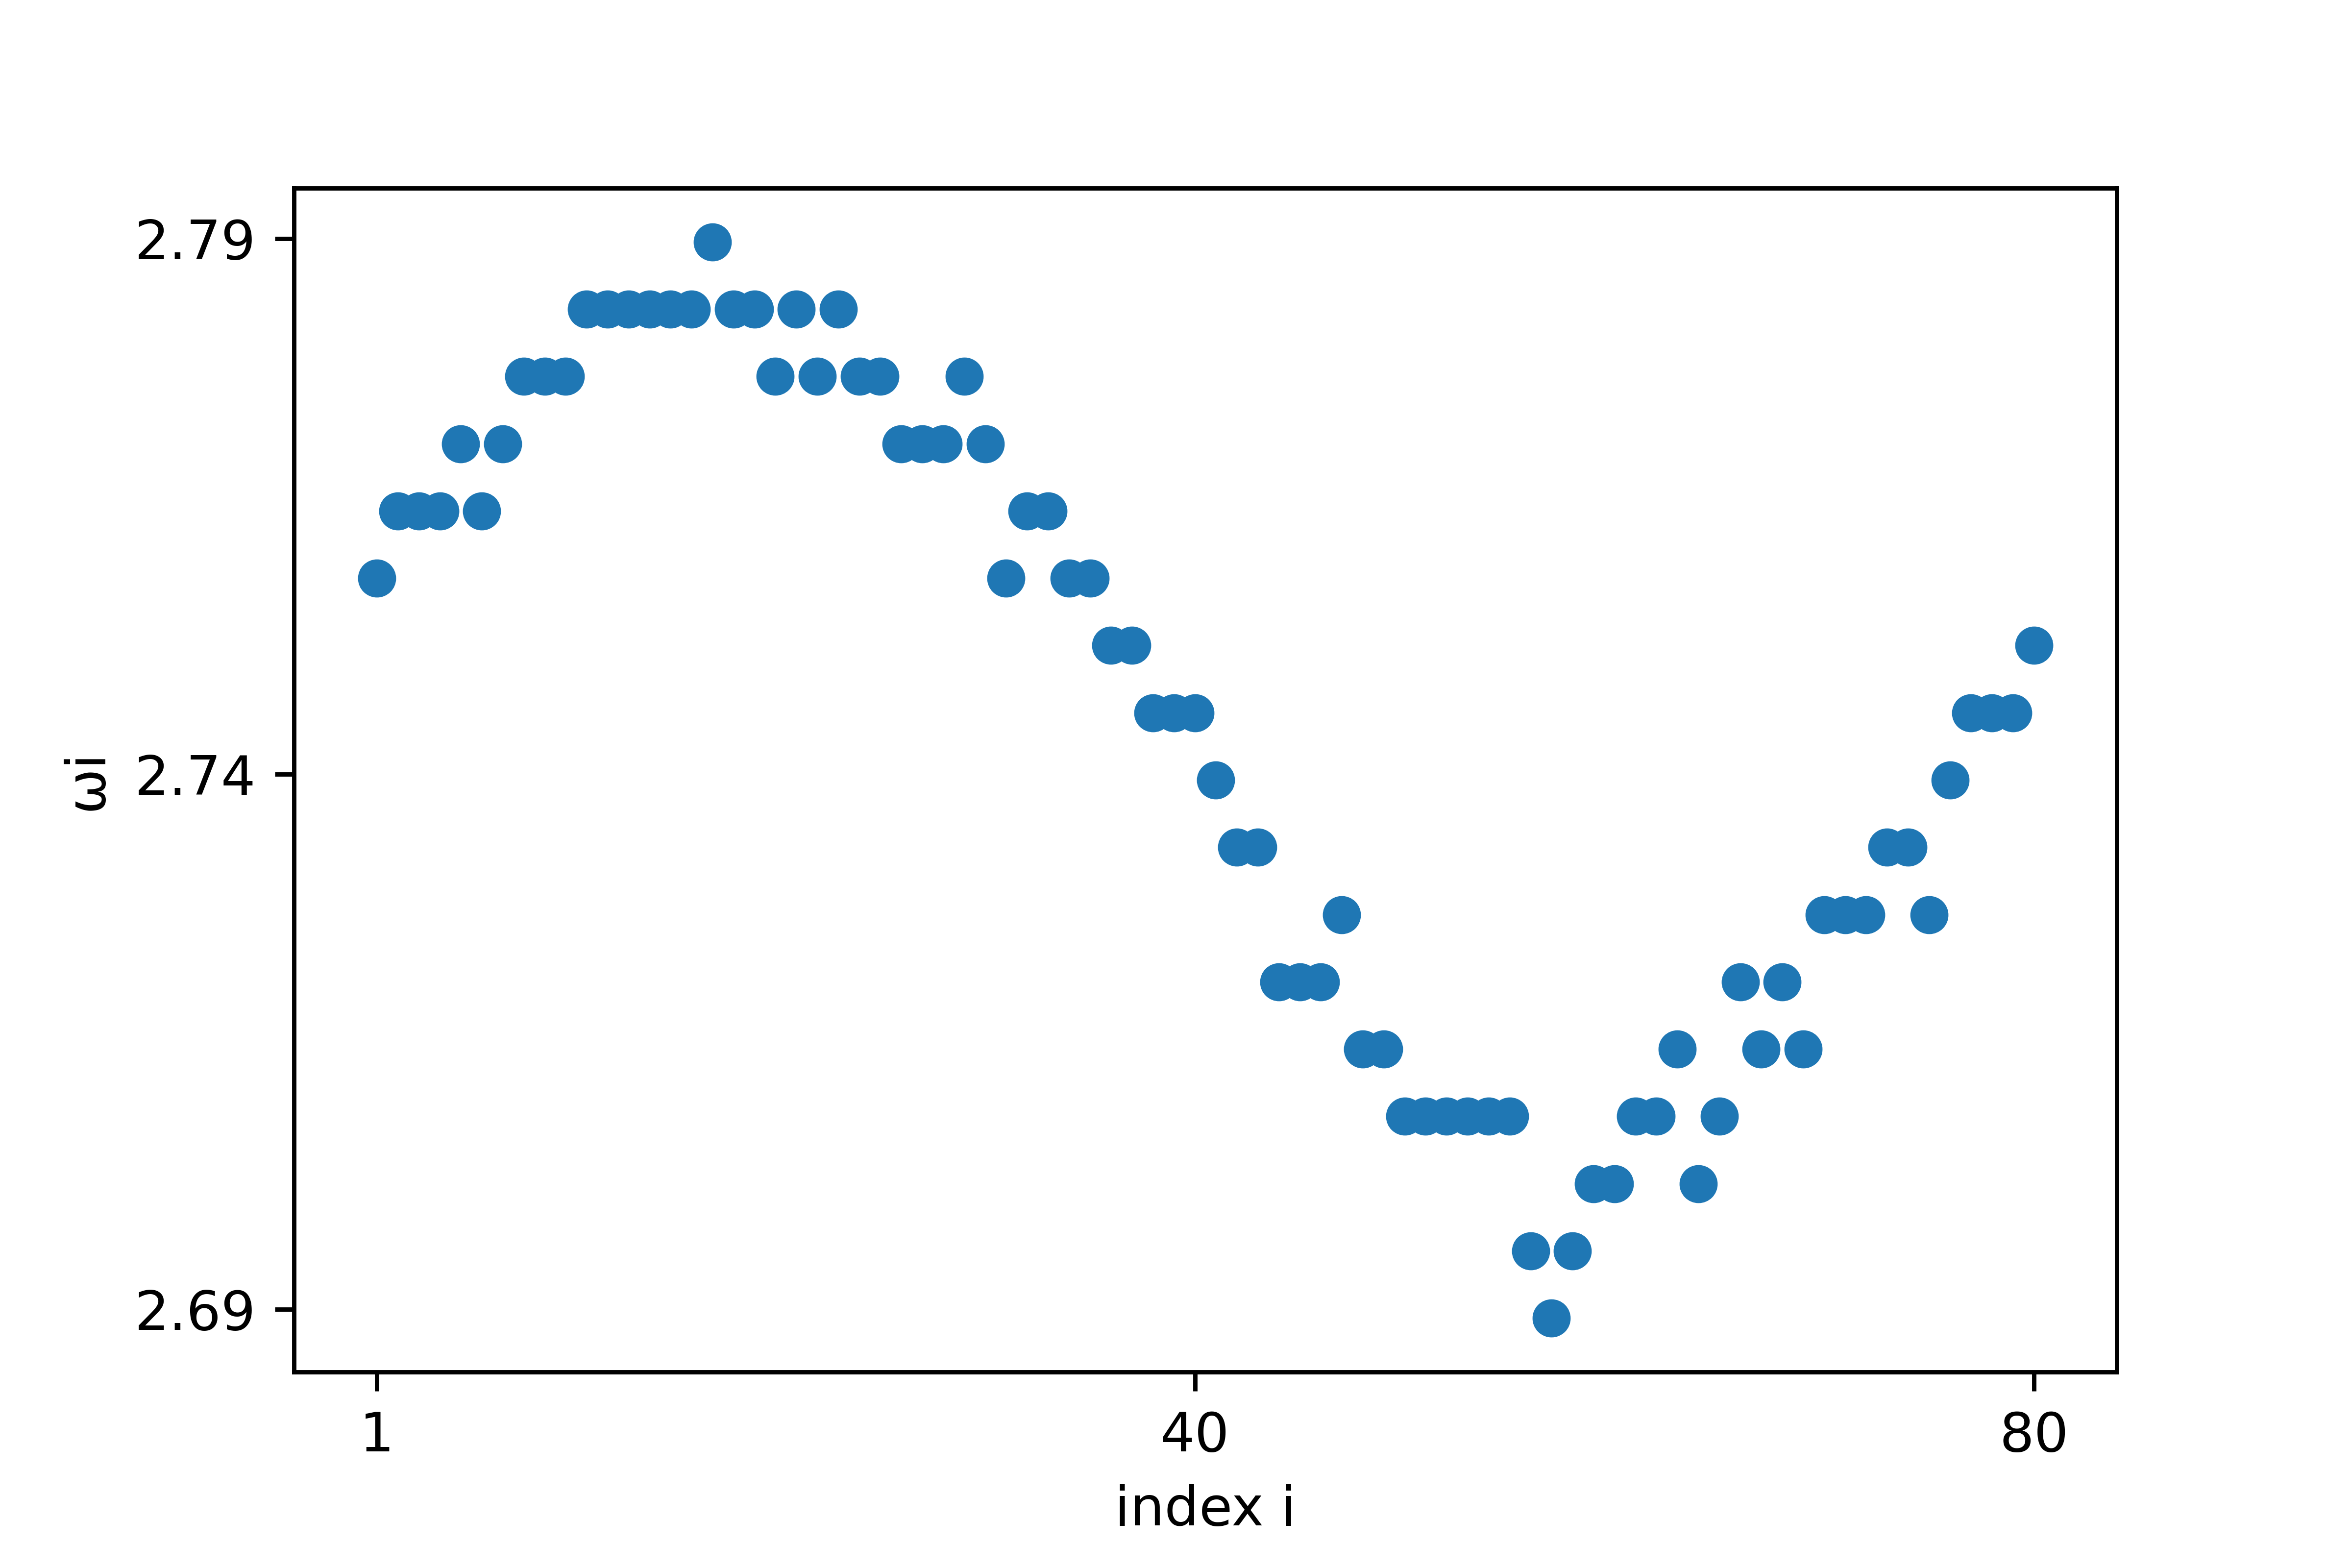
\includegraphics[width=1\linewidth]{w_N=80.png}  
  \caption{$N=80$}
\end{subfigure}
\hfill
\begin{subfigure}{.32\textwidth}
  \centering
  % include first image
  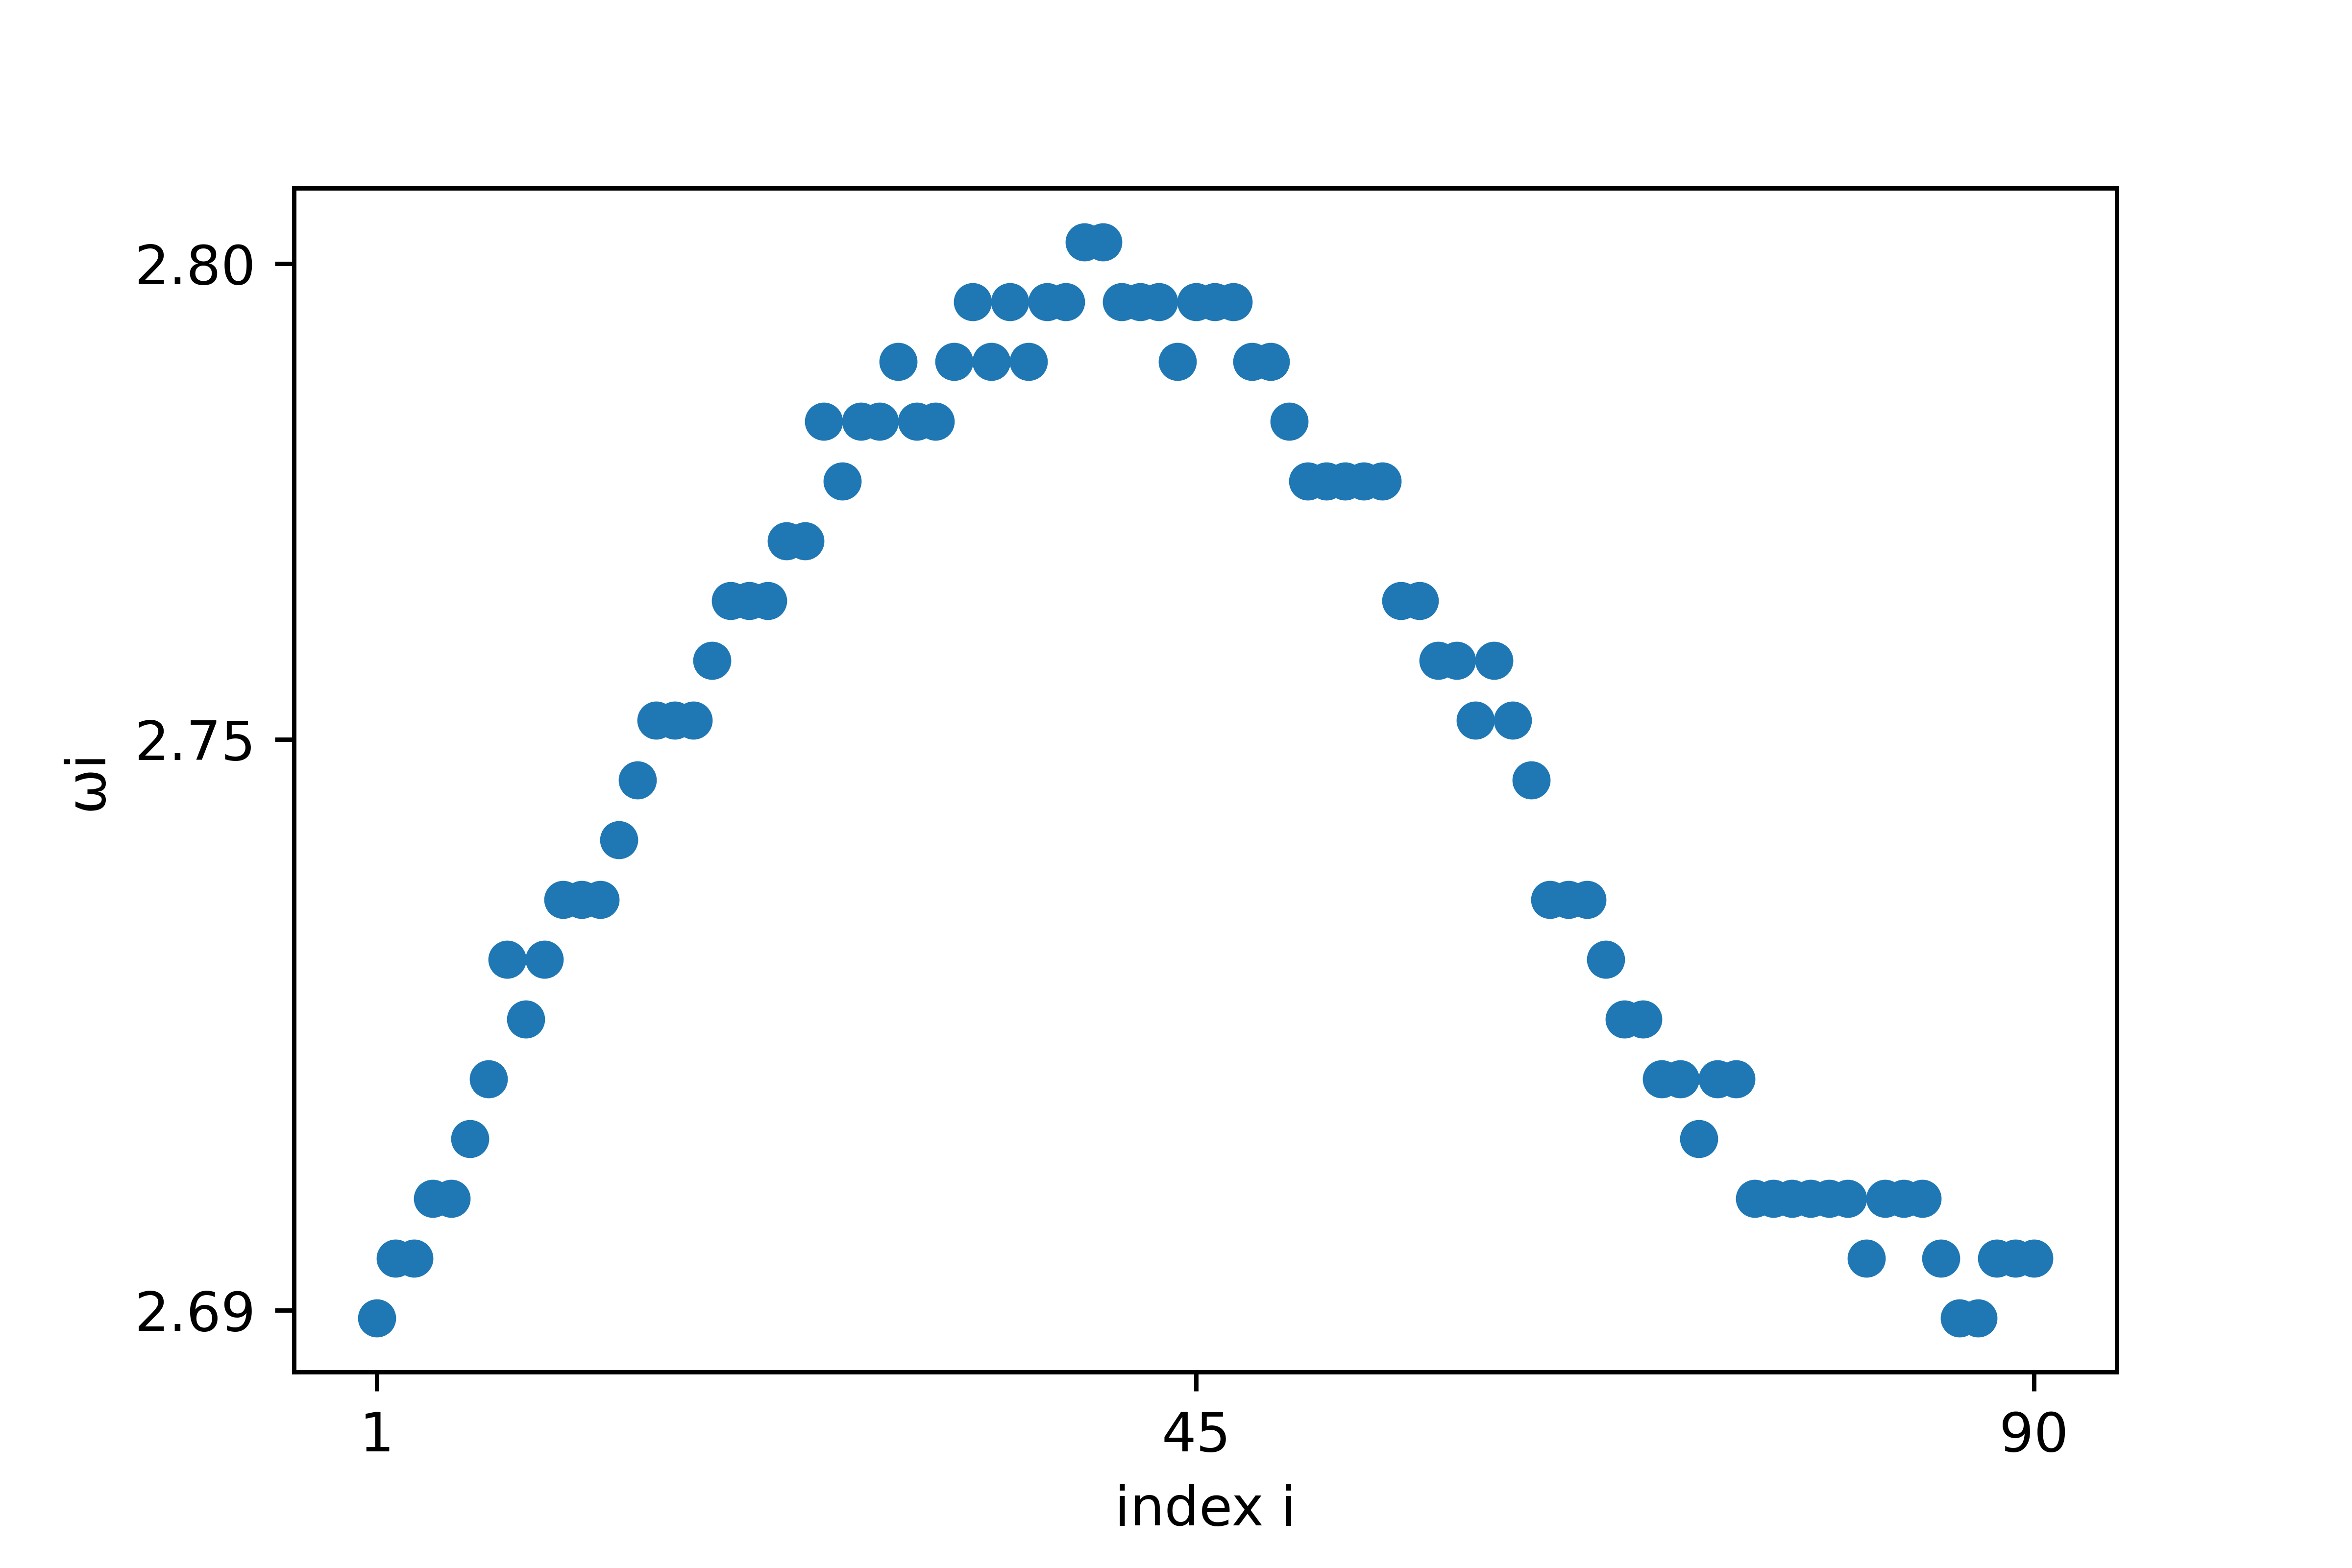
\includegraphics[width=1\linewidth]{w_N=90.png}  
  \caption{$N=90$}
\end{subfigure}
\hfill
\begin{subfigure}{.32\textwidth}
  \centering
  % include first image
  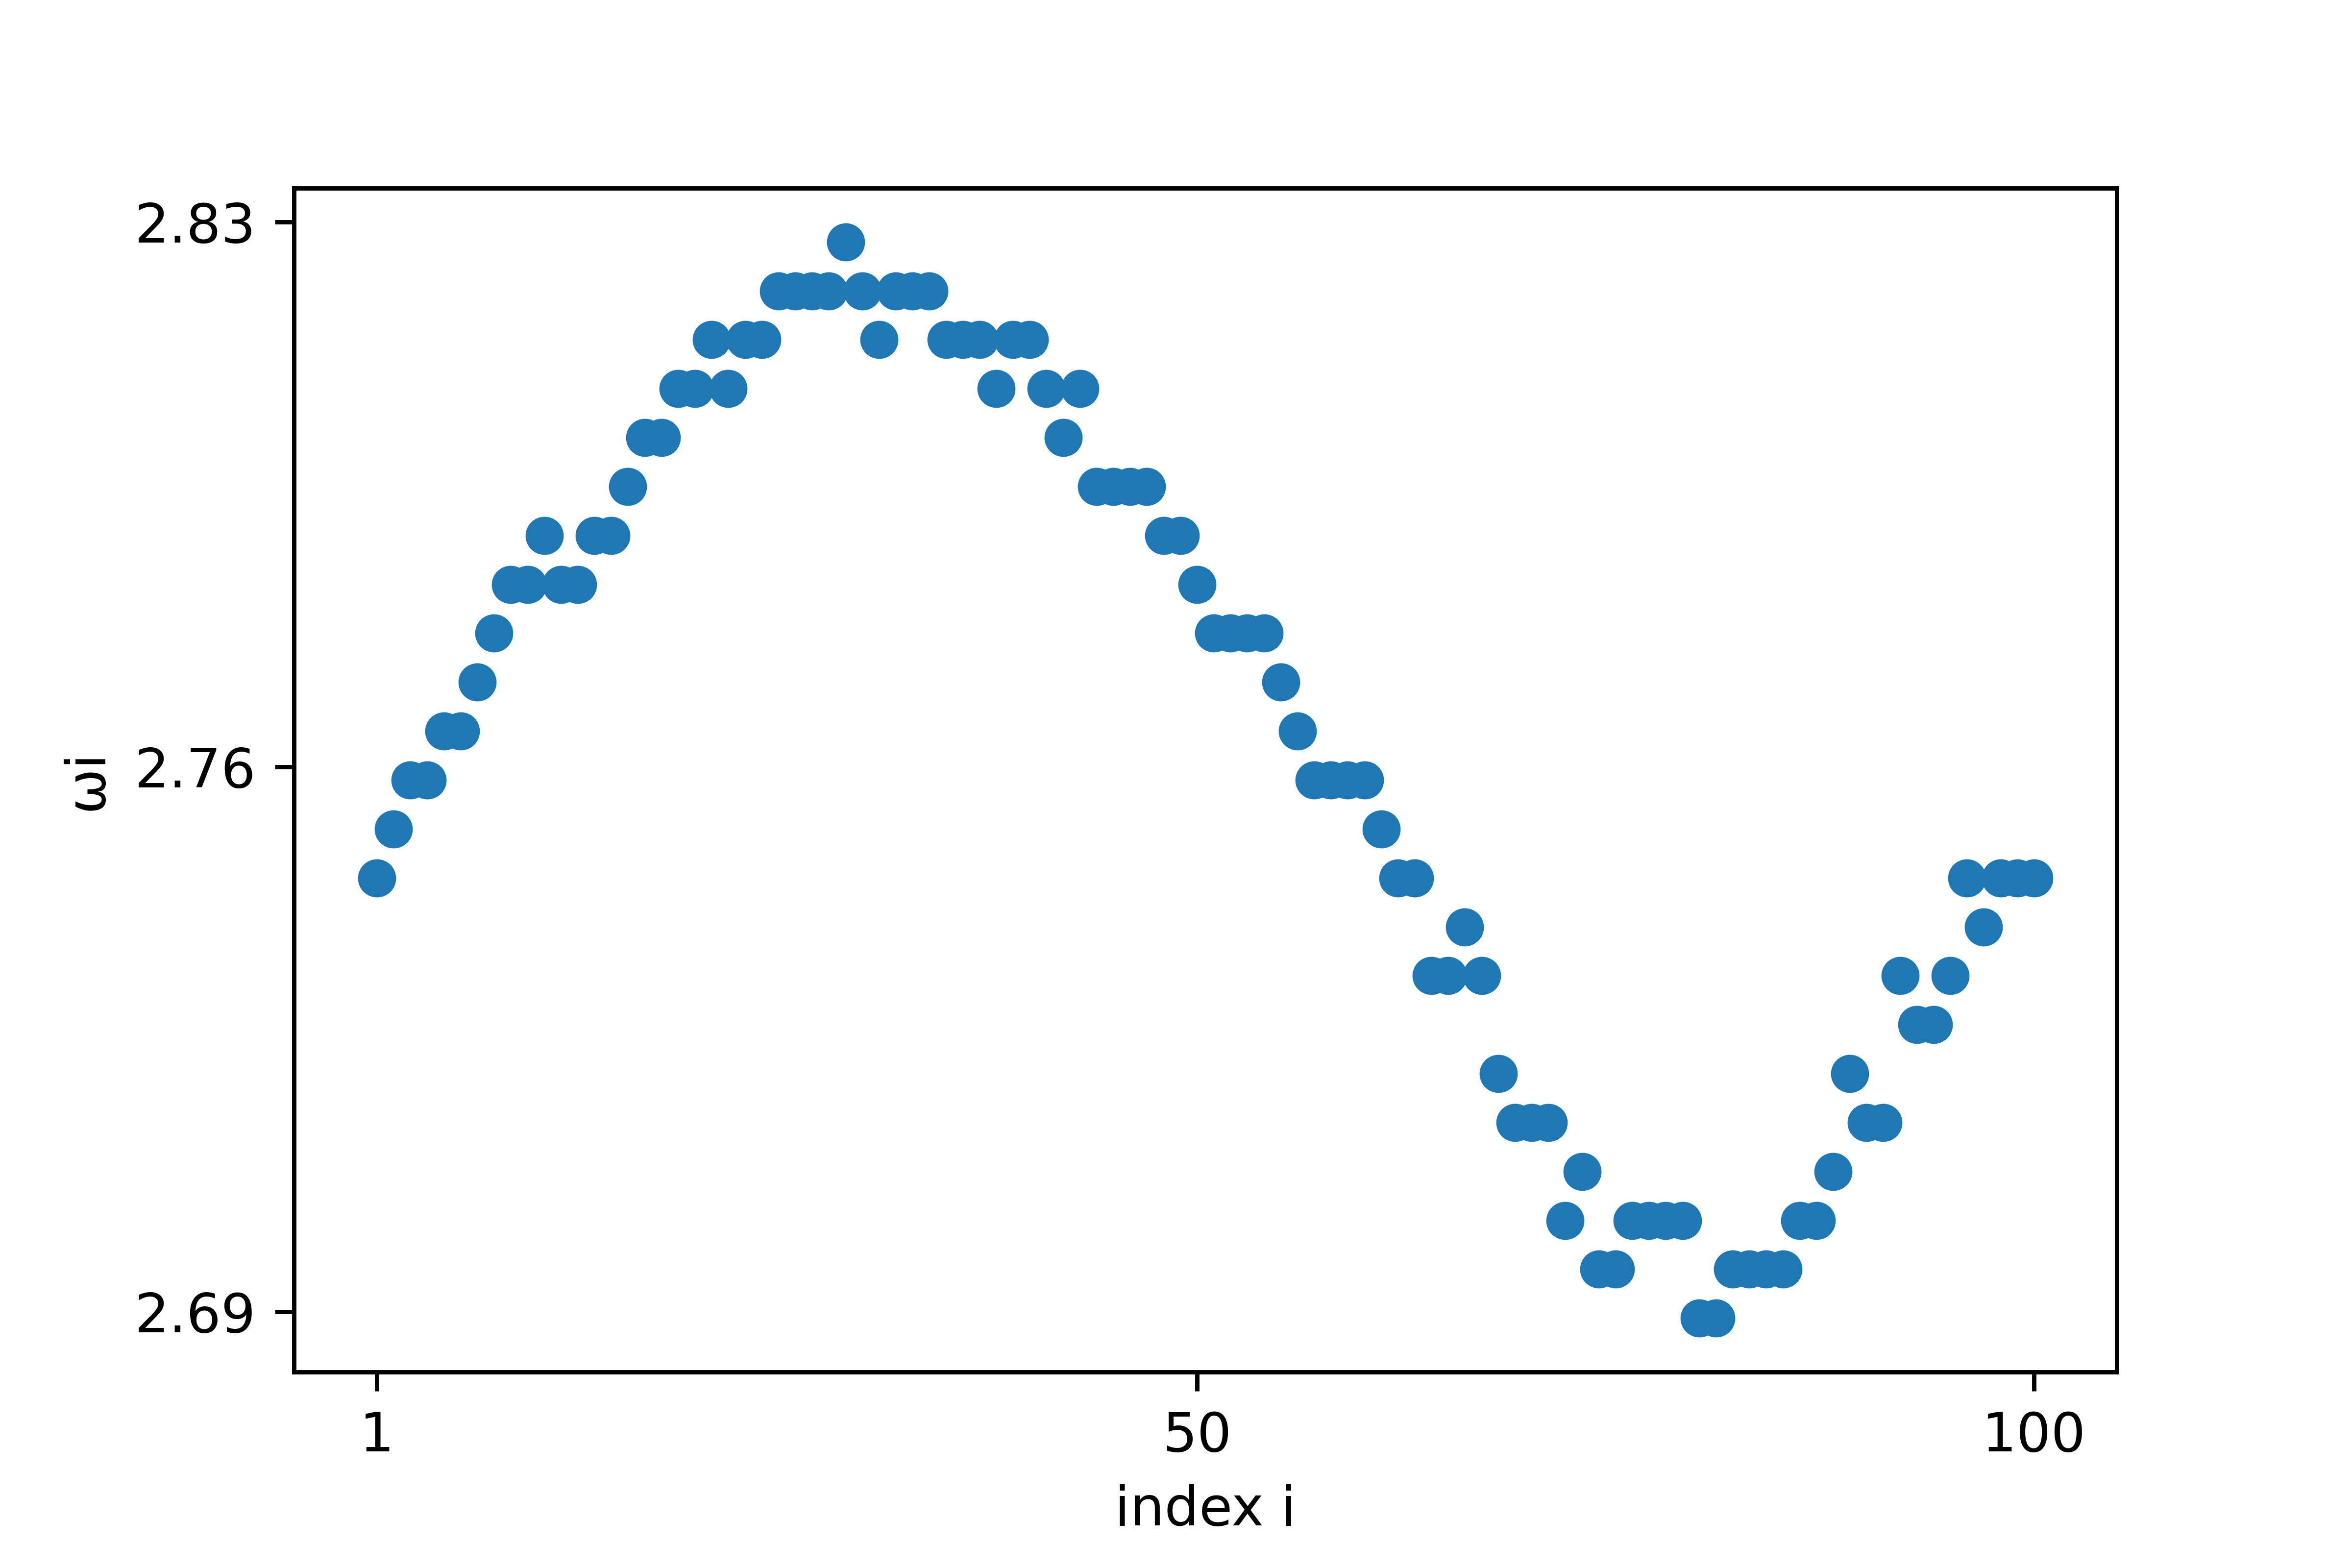
\includegraphics[width=1\linewidth]{w_N=100.png}  
  \caption{$N=100$}
\end{subfigure}
\caption{Mean phase-velocity profiles $\omega_i$ at $t=1000$ time units, for $\sigma = 0.7$, $r=0.40$ and for various values of $N$, as in Fig. (\ref{vsN}).}
\label{vsN2}
\end{figure}
\end{frame}

\begin{frame}{Minimum number of neurons}

\begin{figure}[H]
\centering
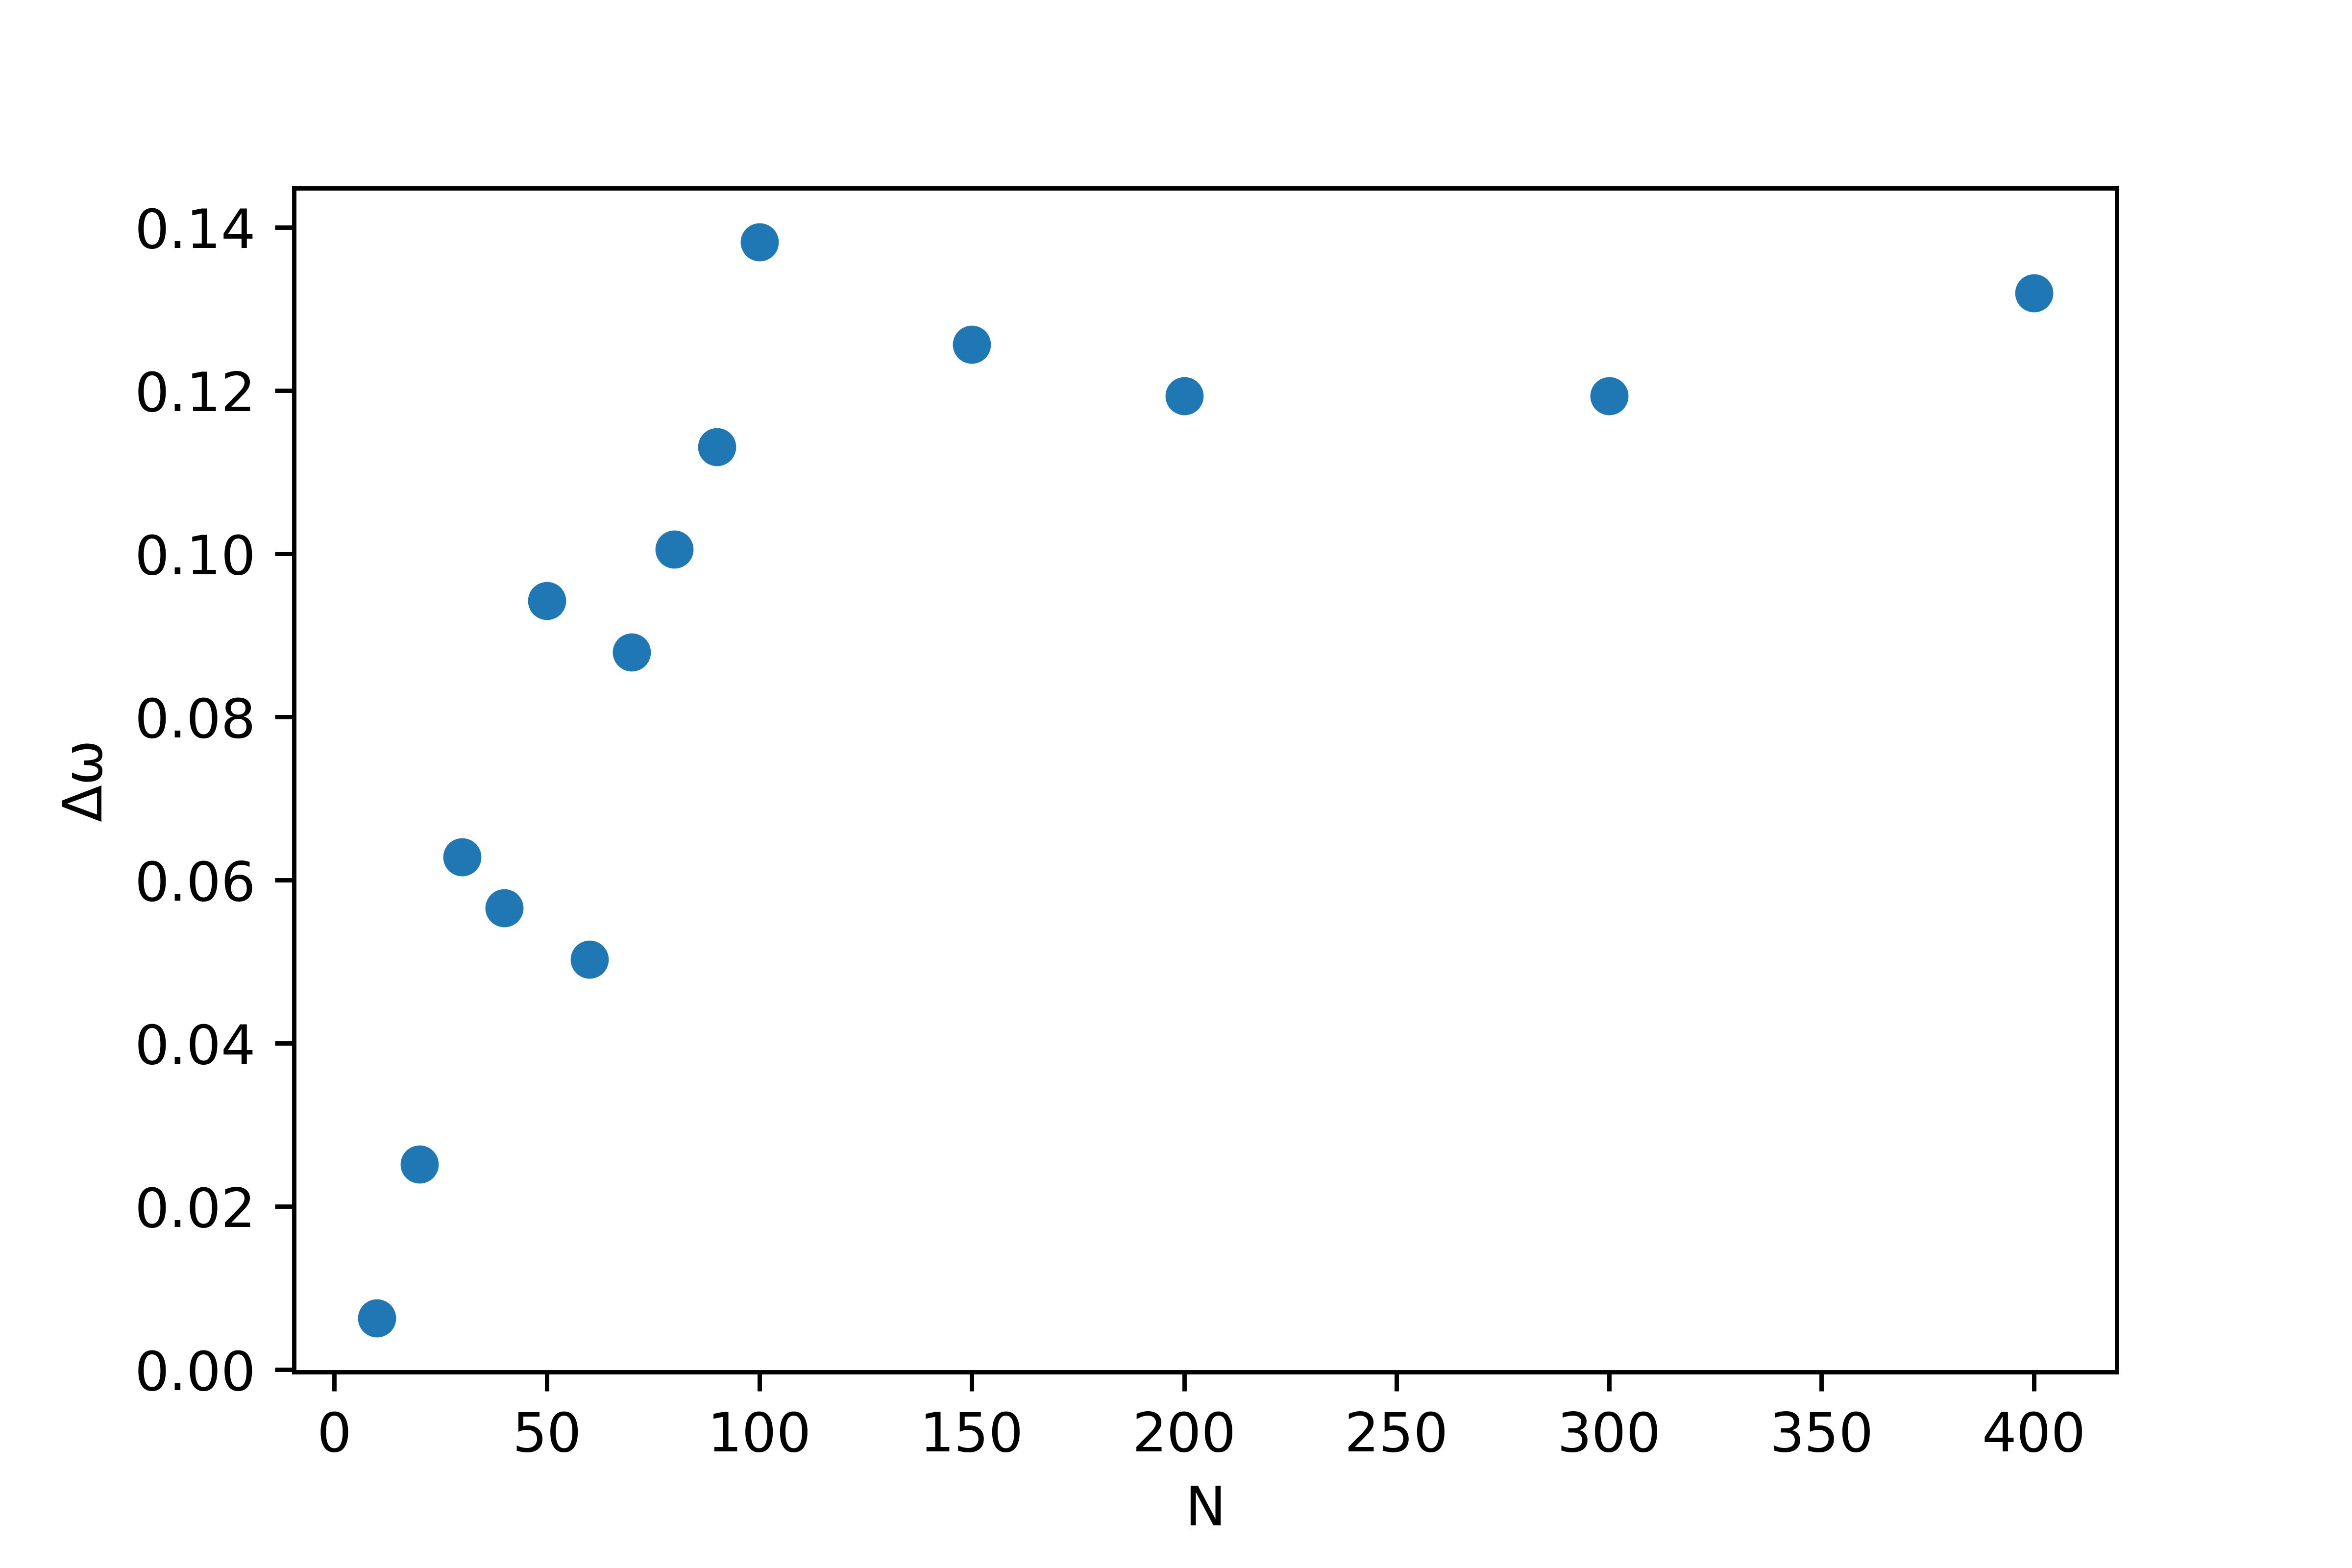
\includegraphics[width=0.6\textwidth]{deltaw_scatter.png}
\caption{$\Delta \omega = \omega_{\text{max}}-\omega_{\text{min}}$ with varying system size $N$.}
\label{dw}
\end{figure}
\noindent

\end{frame}

\subsection{Varying $\sigma$}
\begin{frame}{Varying $\sigma$} \pause
\begin{figure}[H]
\begin{subfigure}{.32\textwidth}
  \centering
  % include first image
  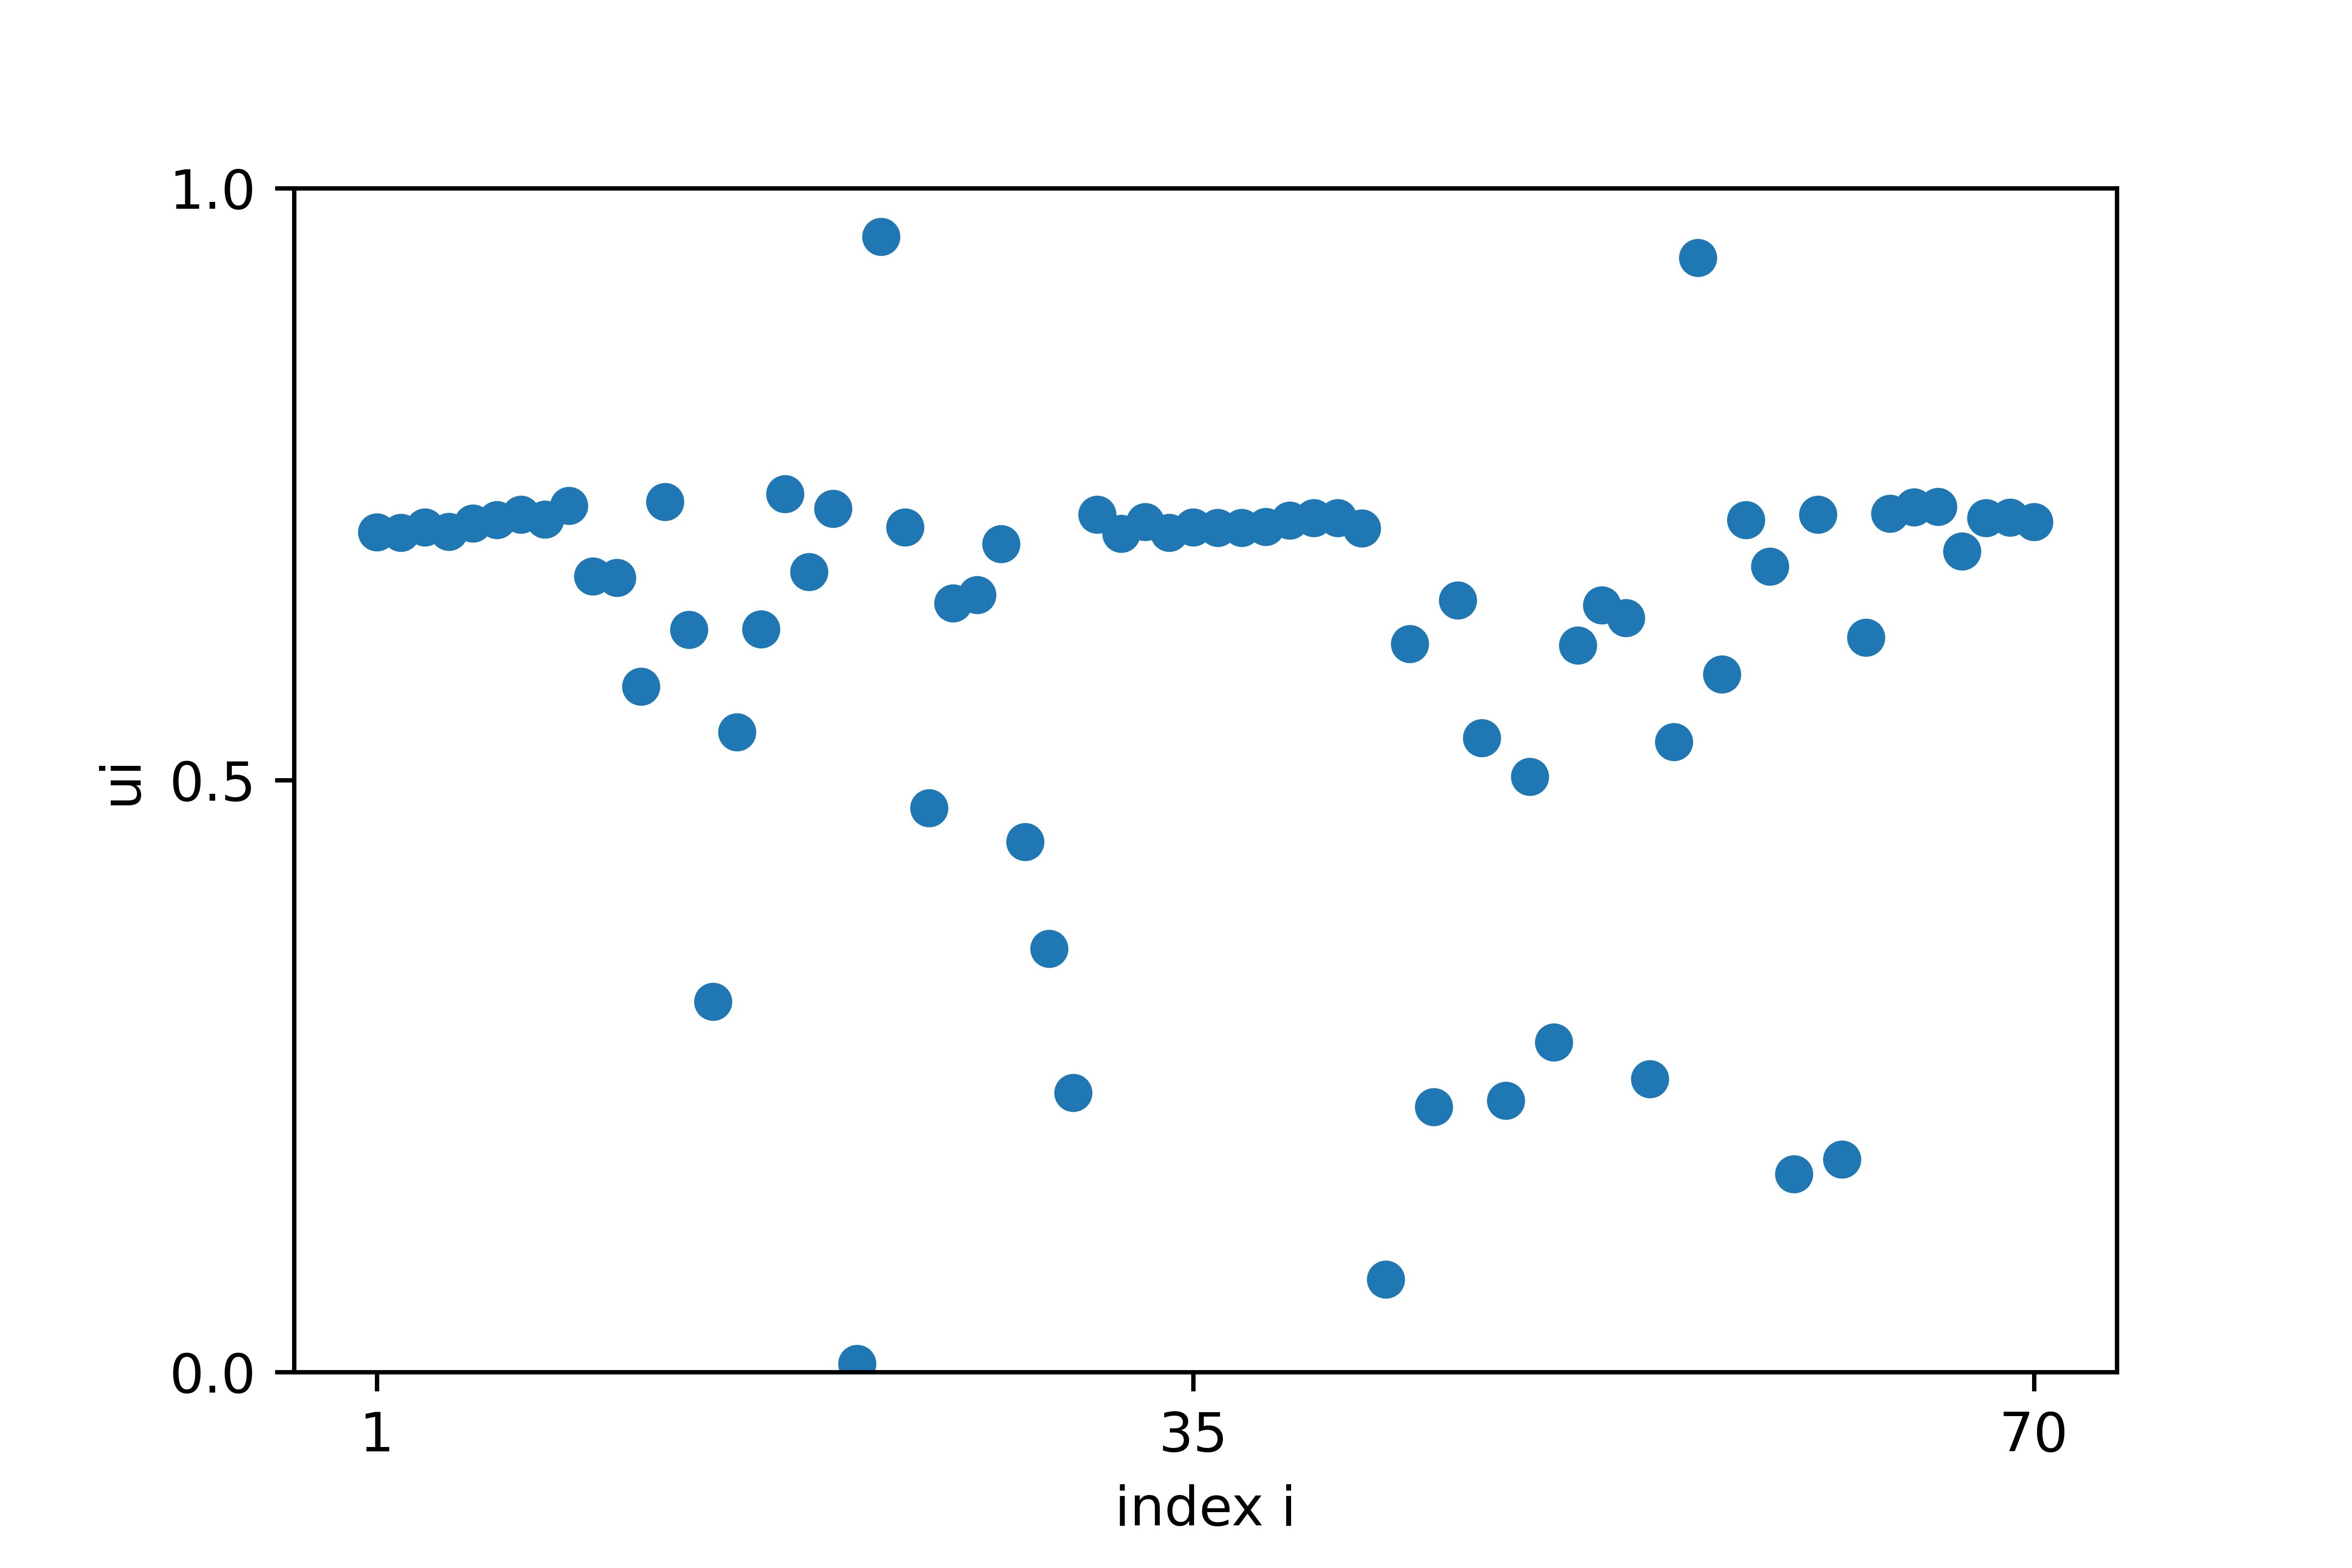
\includegraphics[width=1\linewidth]{u_sigma=1.5.png}  
  \caption{$\sigma = 1.5$}
\end{subfigure}
\hfill
\begin{subfigure}{.32\textwidth}
  \centering
  % include second image
  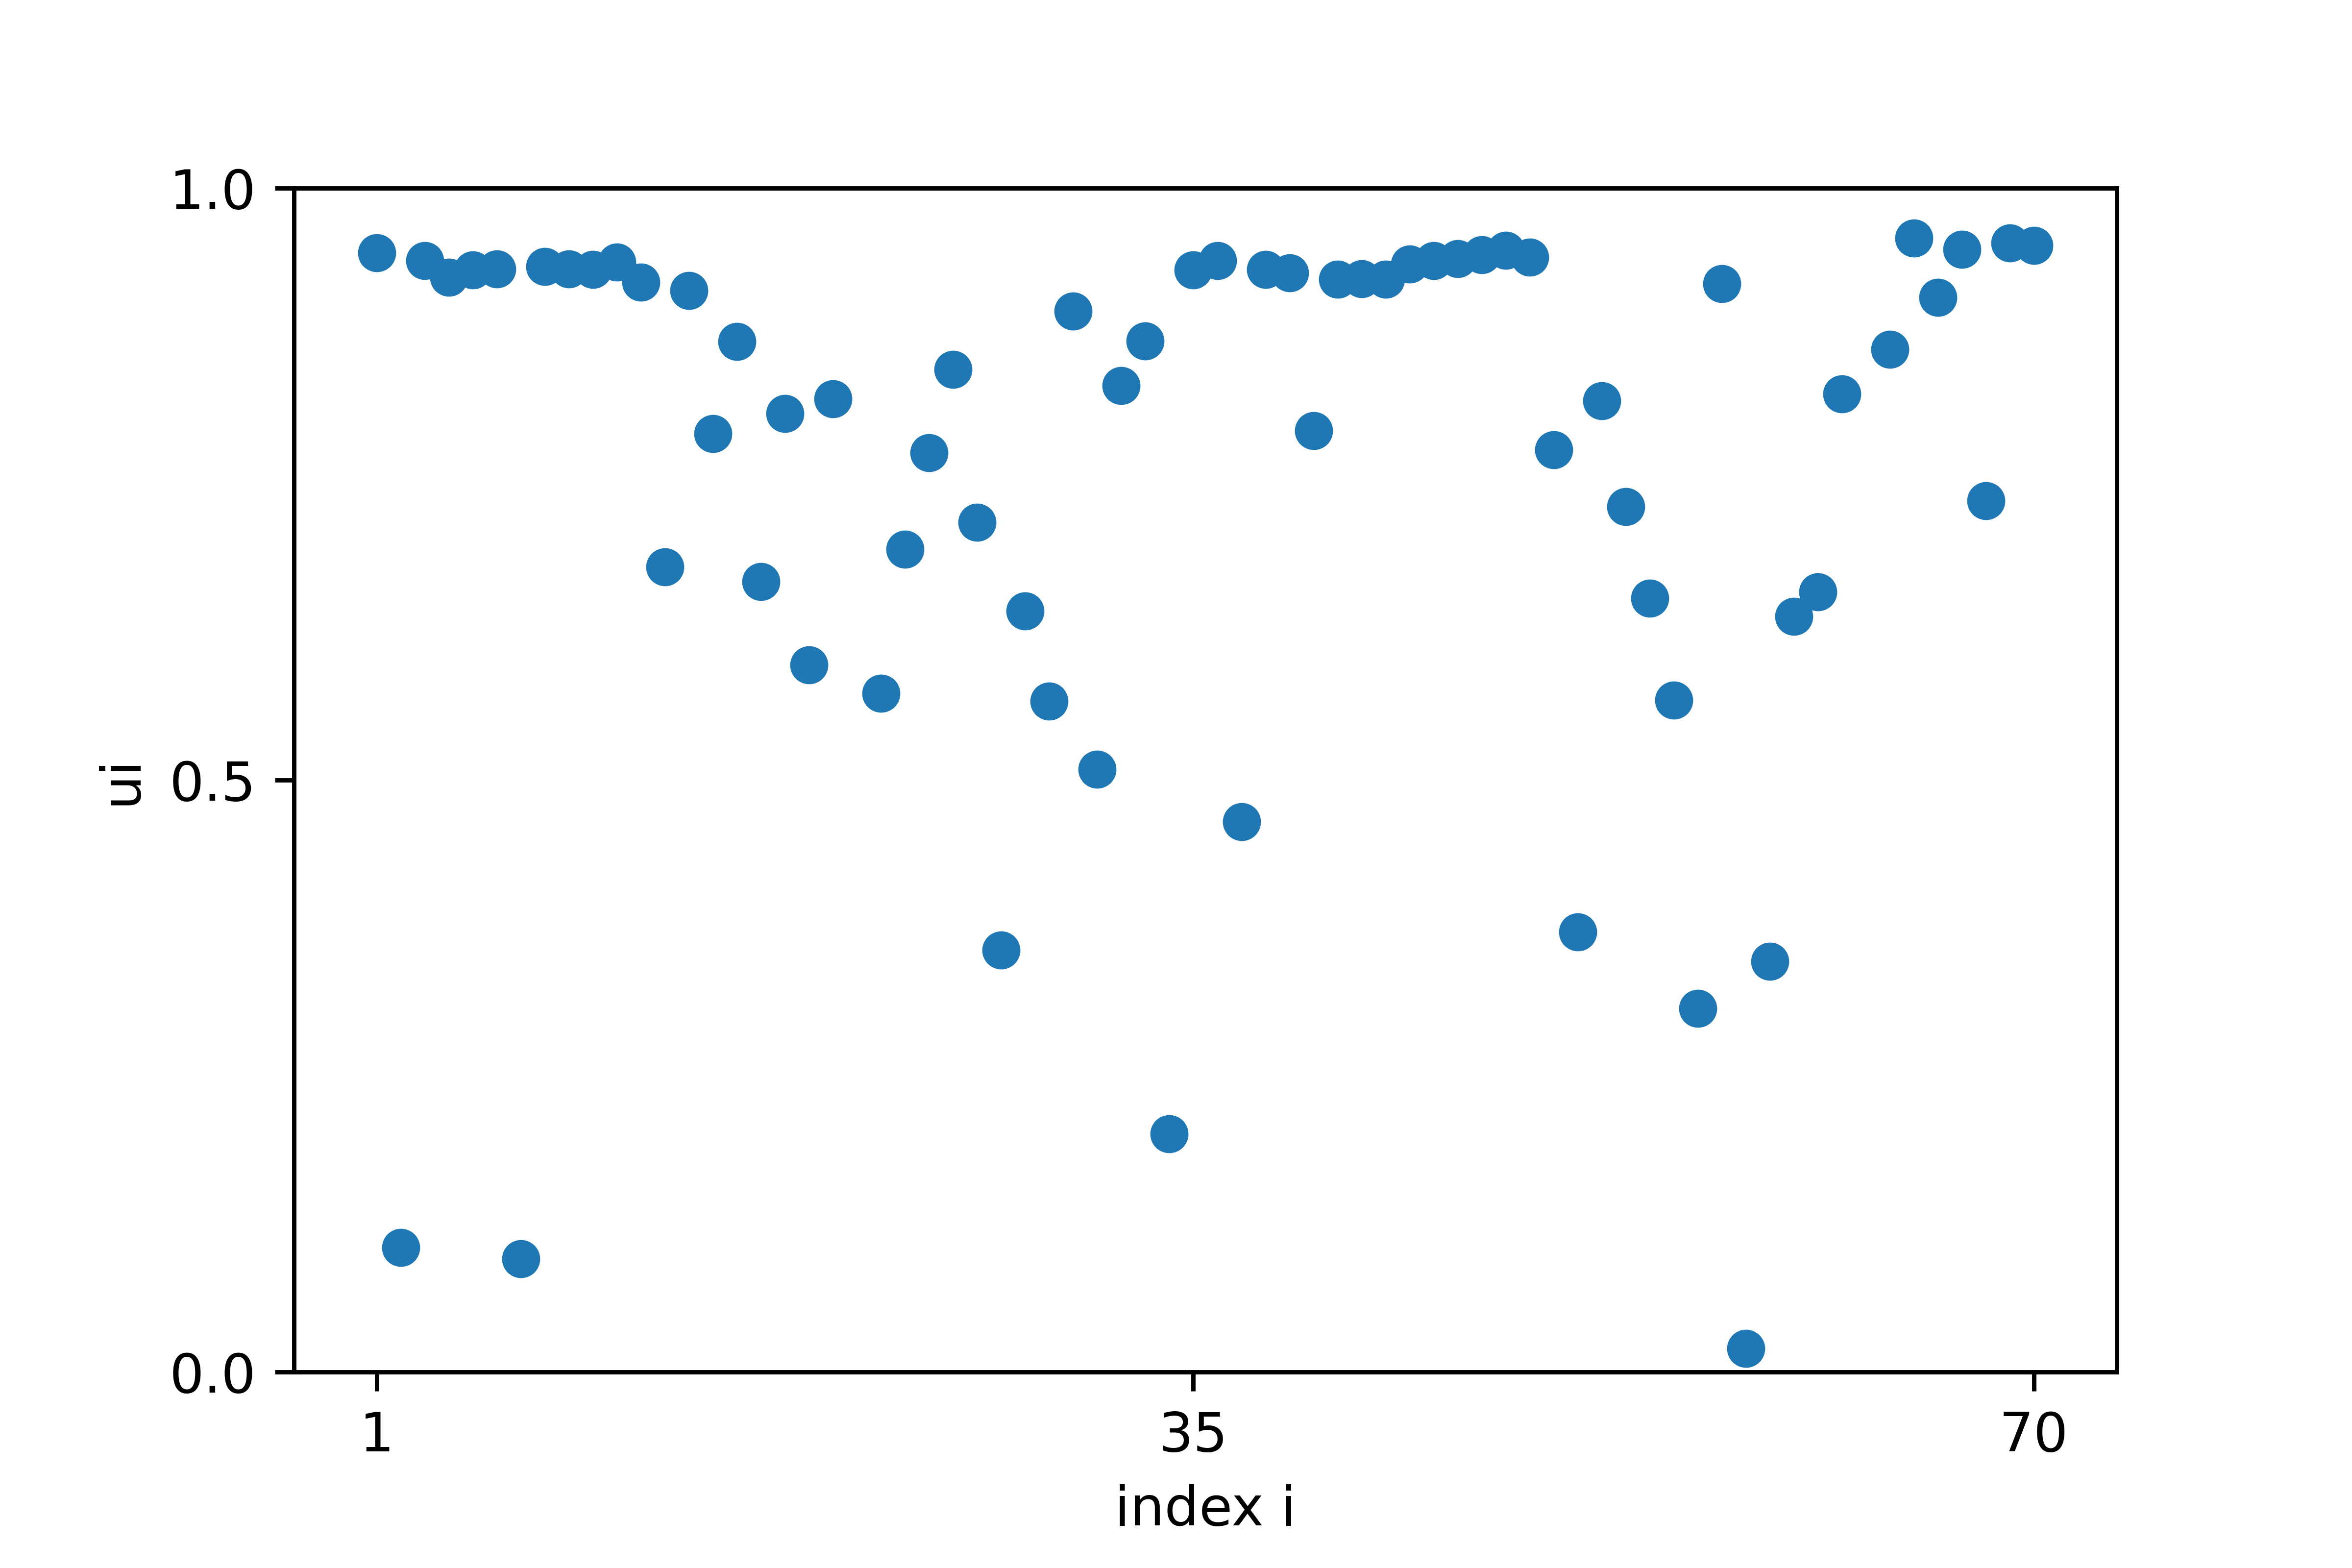
\includegraphics[width=1\linewidth]{u_sigma=1.6.png}  
  \caption{$\sigma = 1.6$}
\end{subfigure}
\hfill
\begin{subfigure}{.32\textwidth}
  \centering
  % include first image
  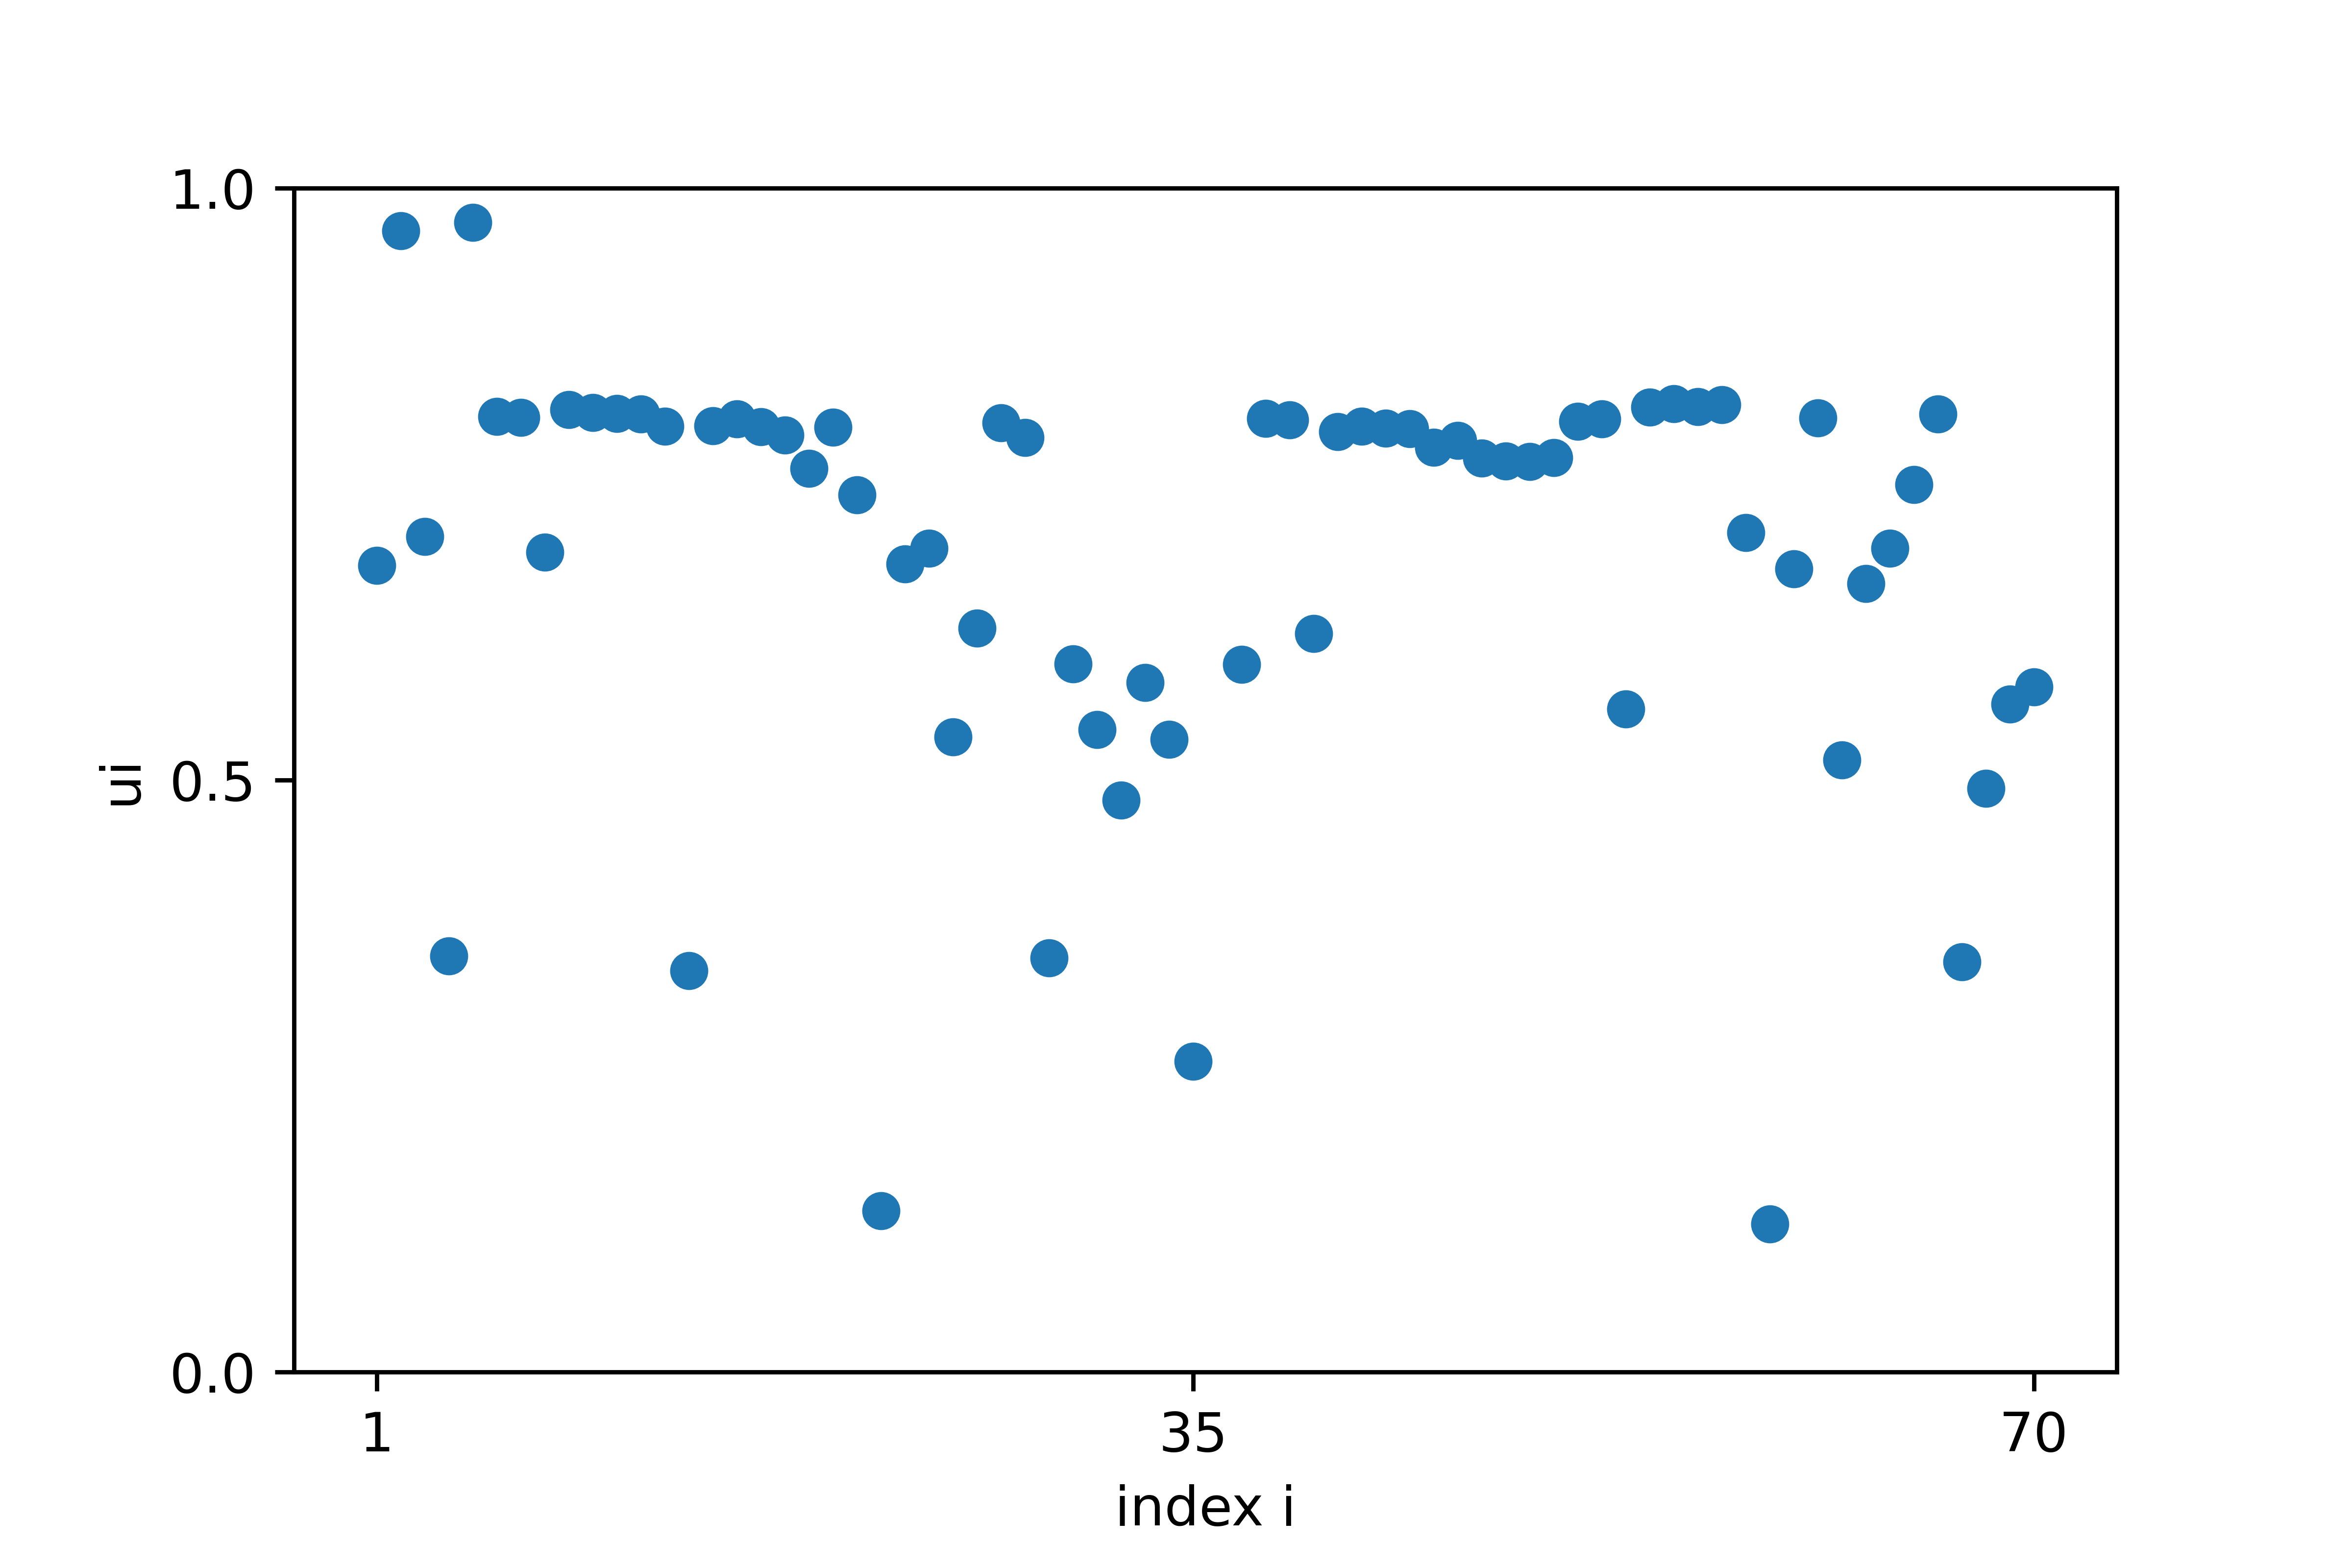
\includegraphics[width=1\linewidth]{u_sigma=1.7.png}  
  \caption{$\sigma = 1.7$}
\end{subfigure}
\begin{subfigure}{.32\textwidth}
  \centering
  % include first image
  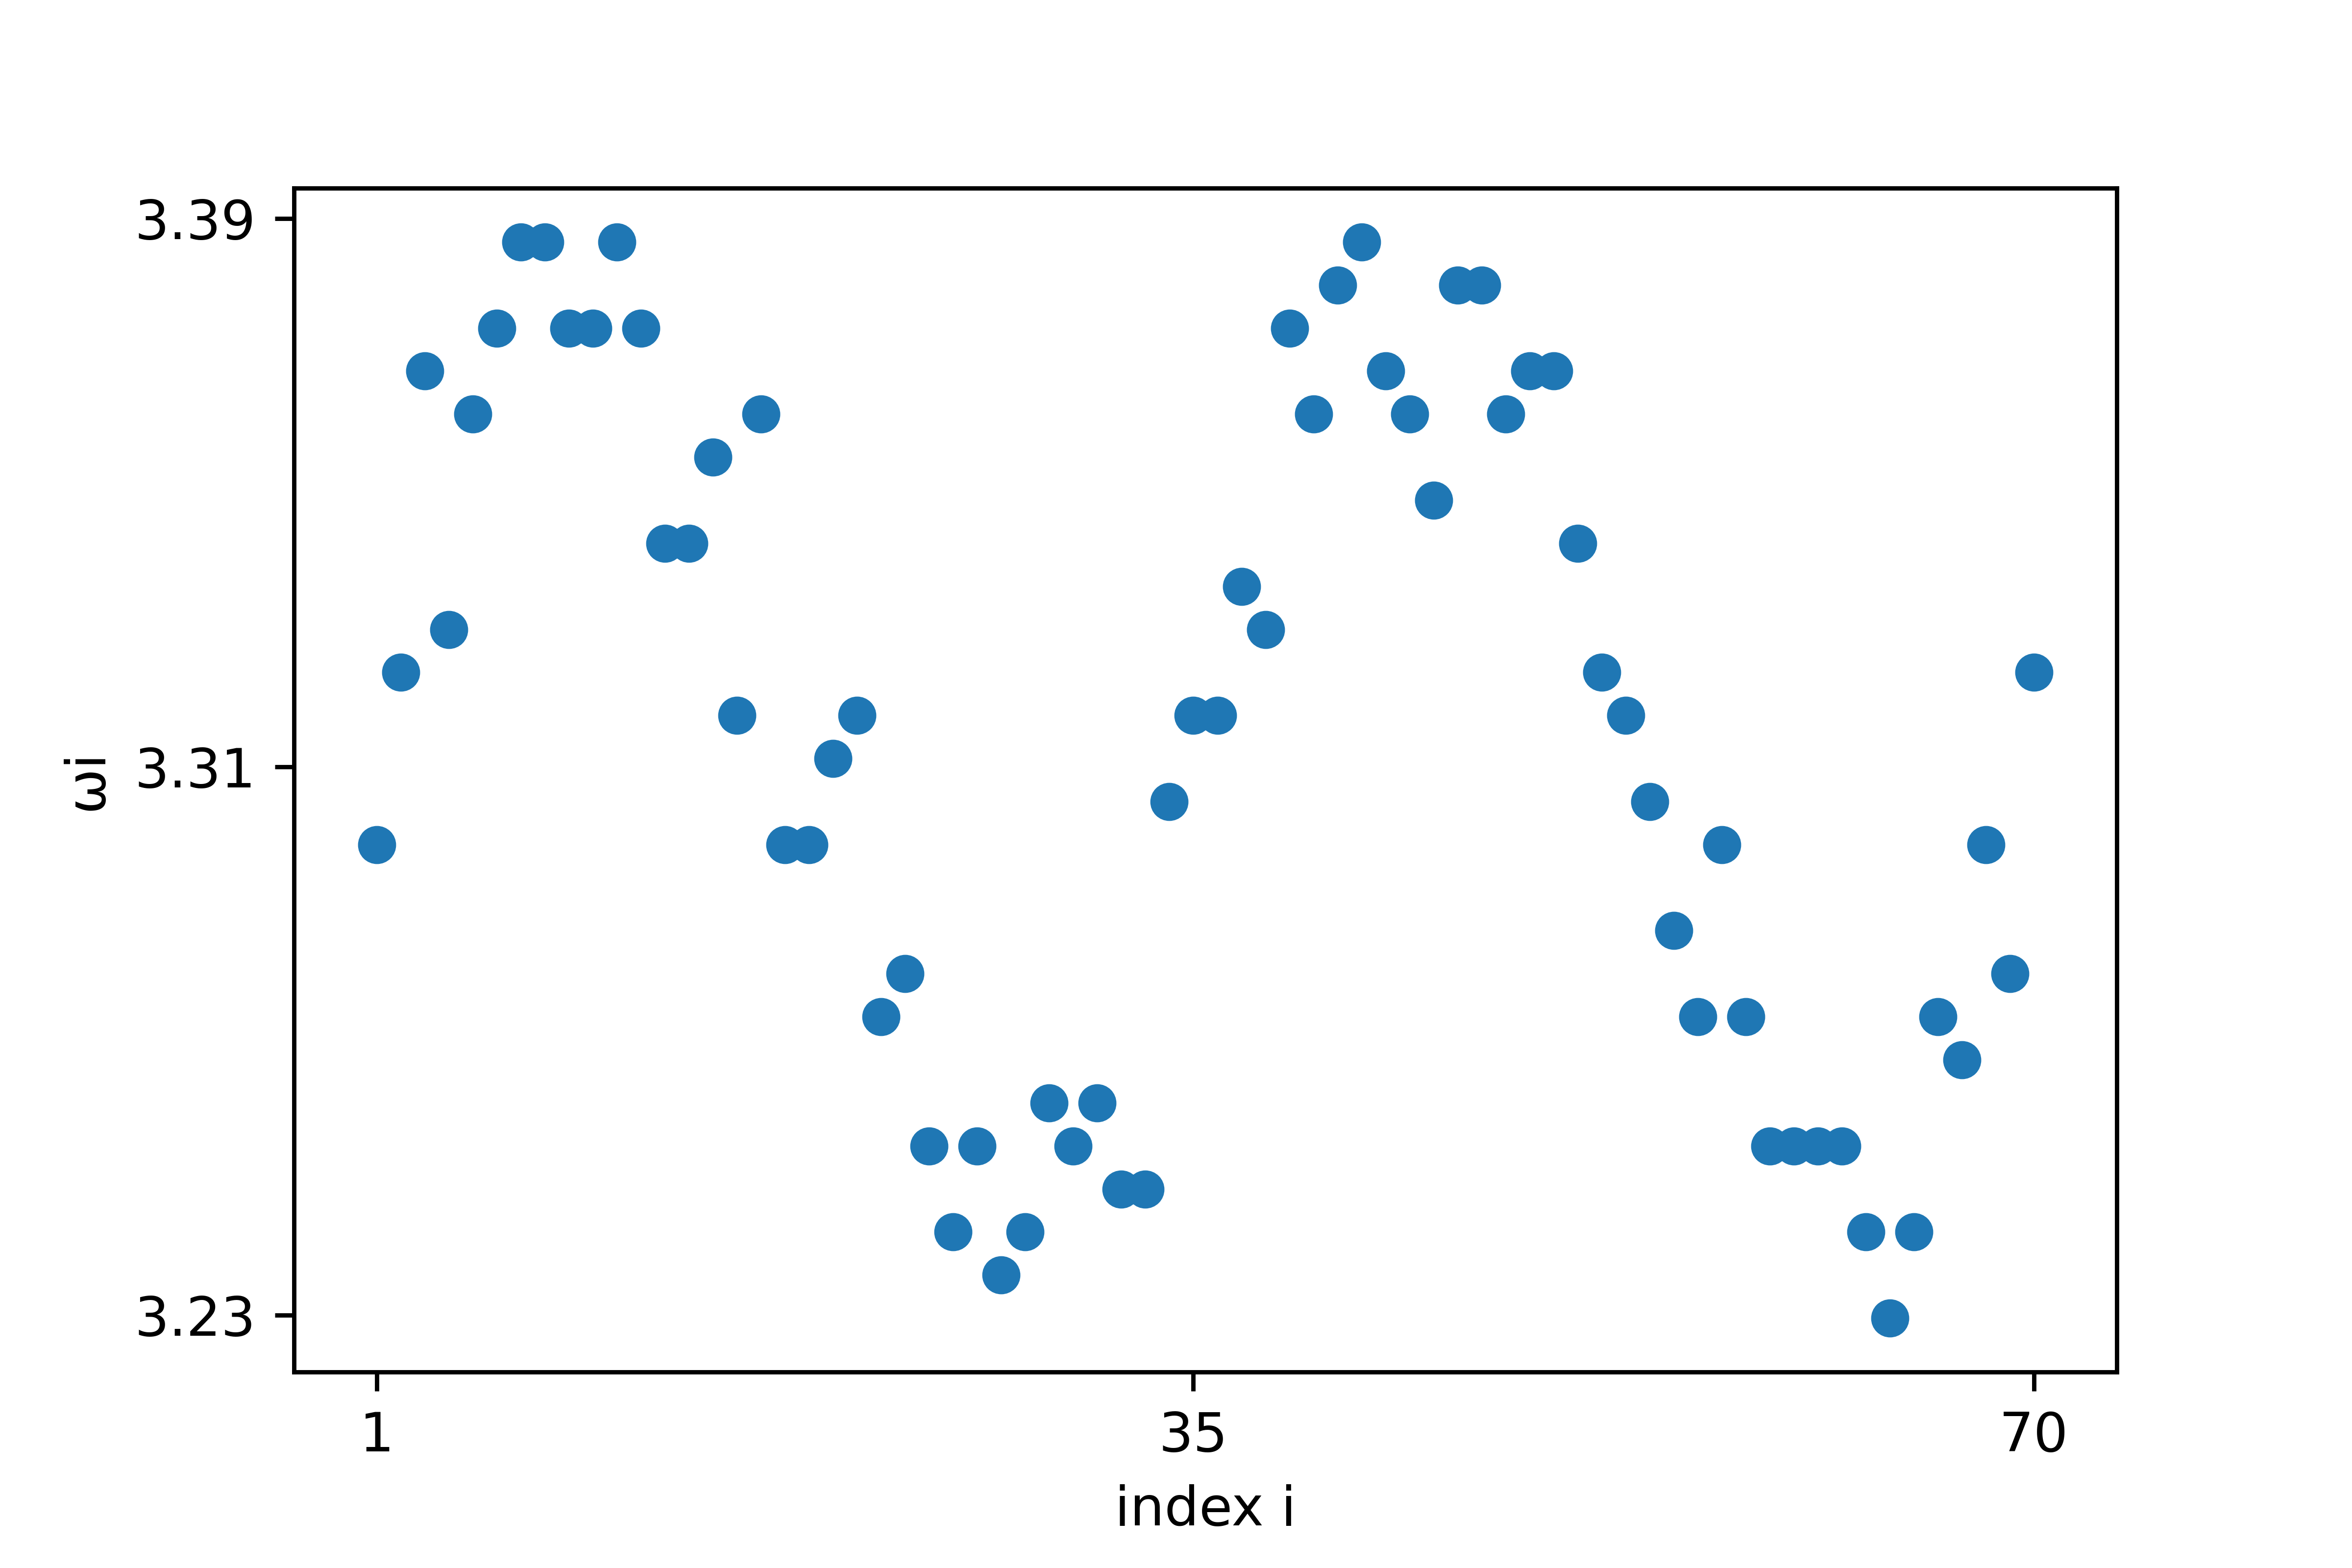
\includegraphics[width=1\linewidth]{w_sigma=1.5.png}  
  \caption{$\sigma = 1.5$}
\end{subfigure}
\hfill
\begin{subfigure}{.32\textwidth}
  \centering
  % include first image
  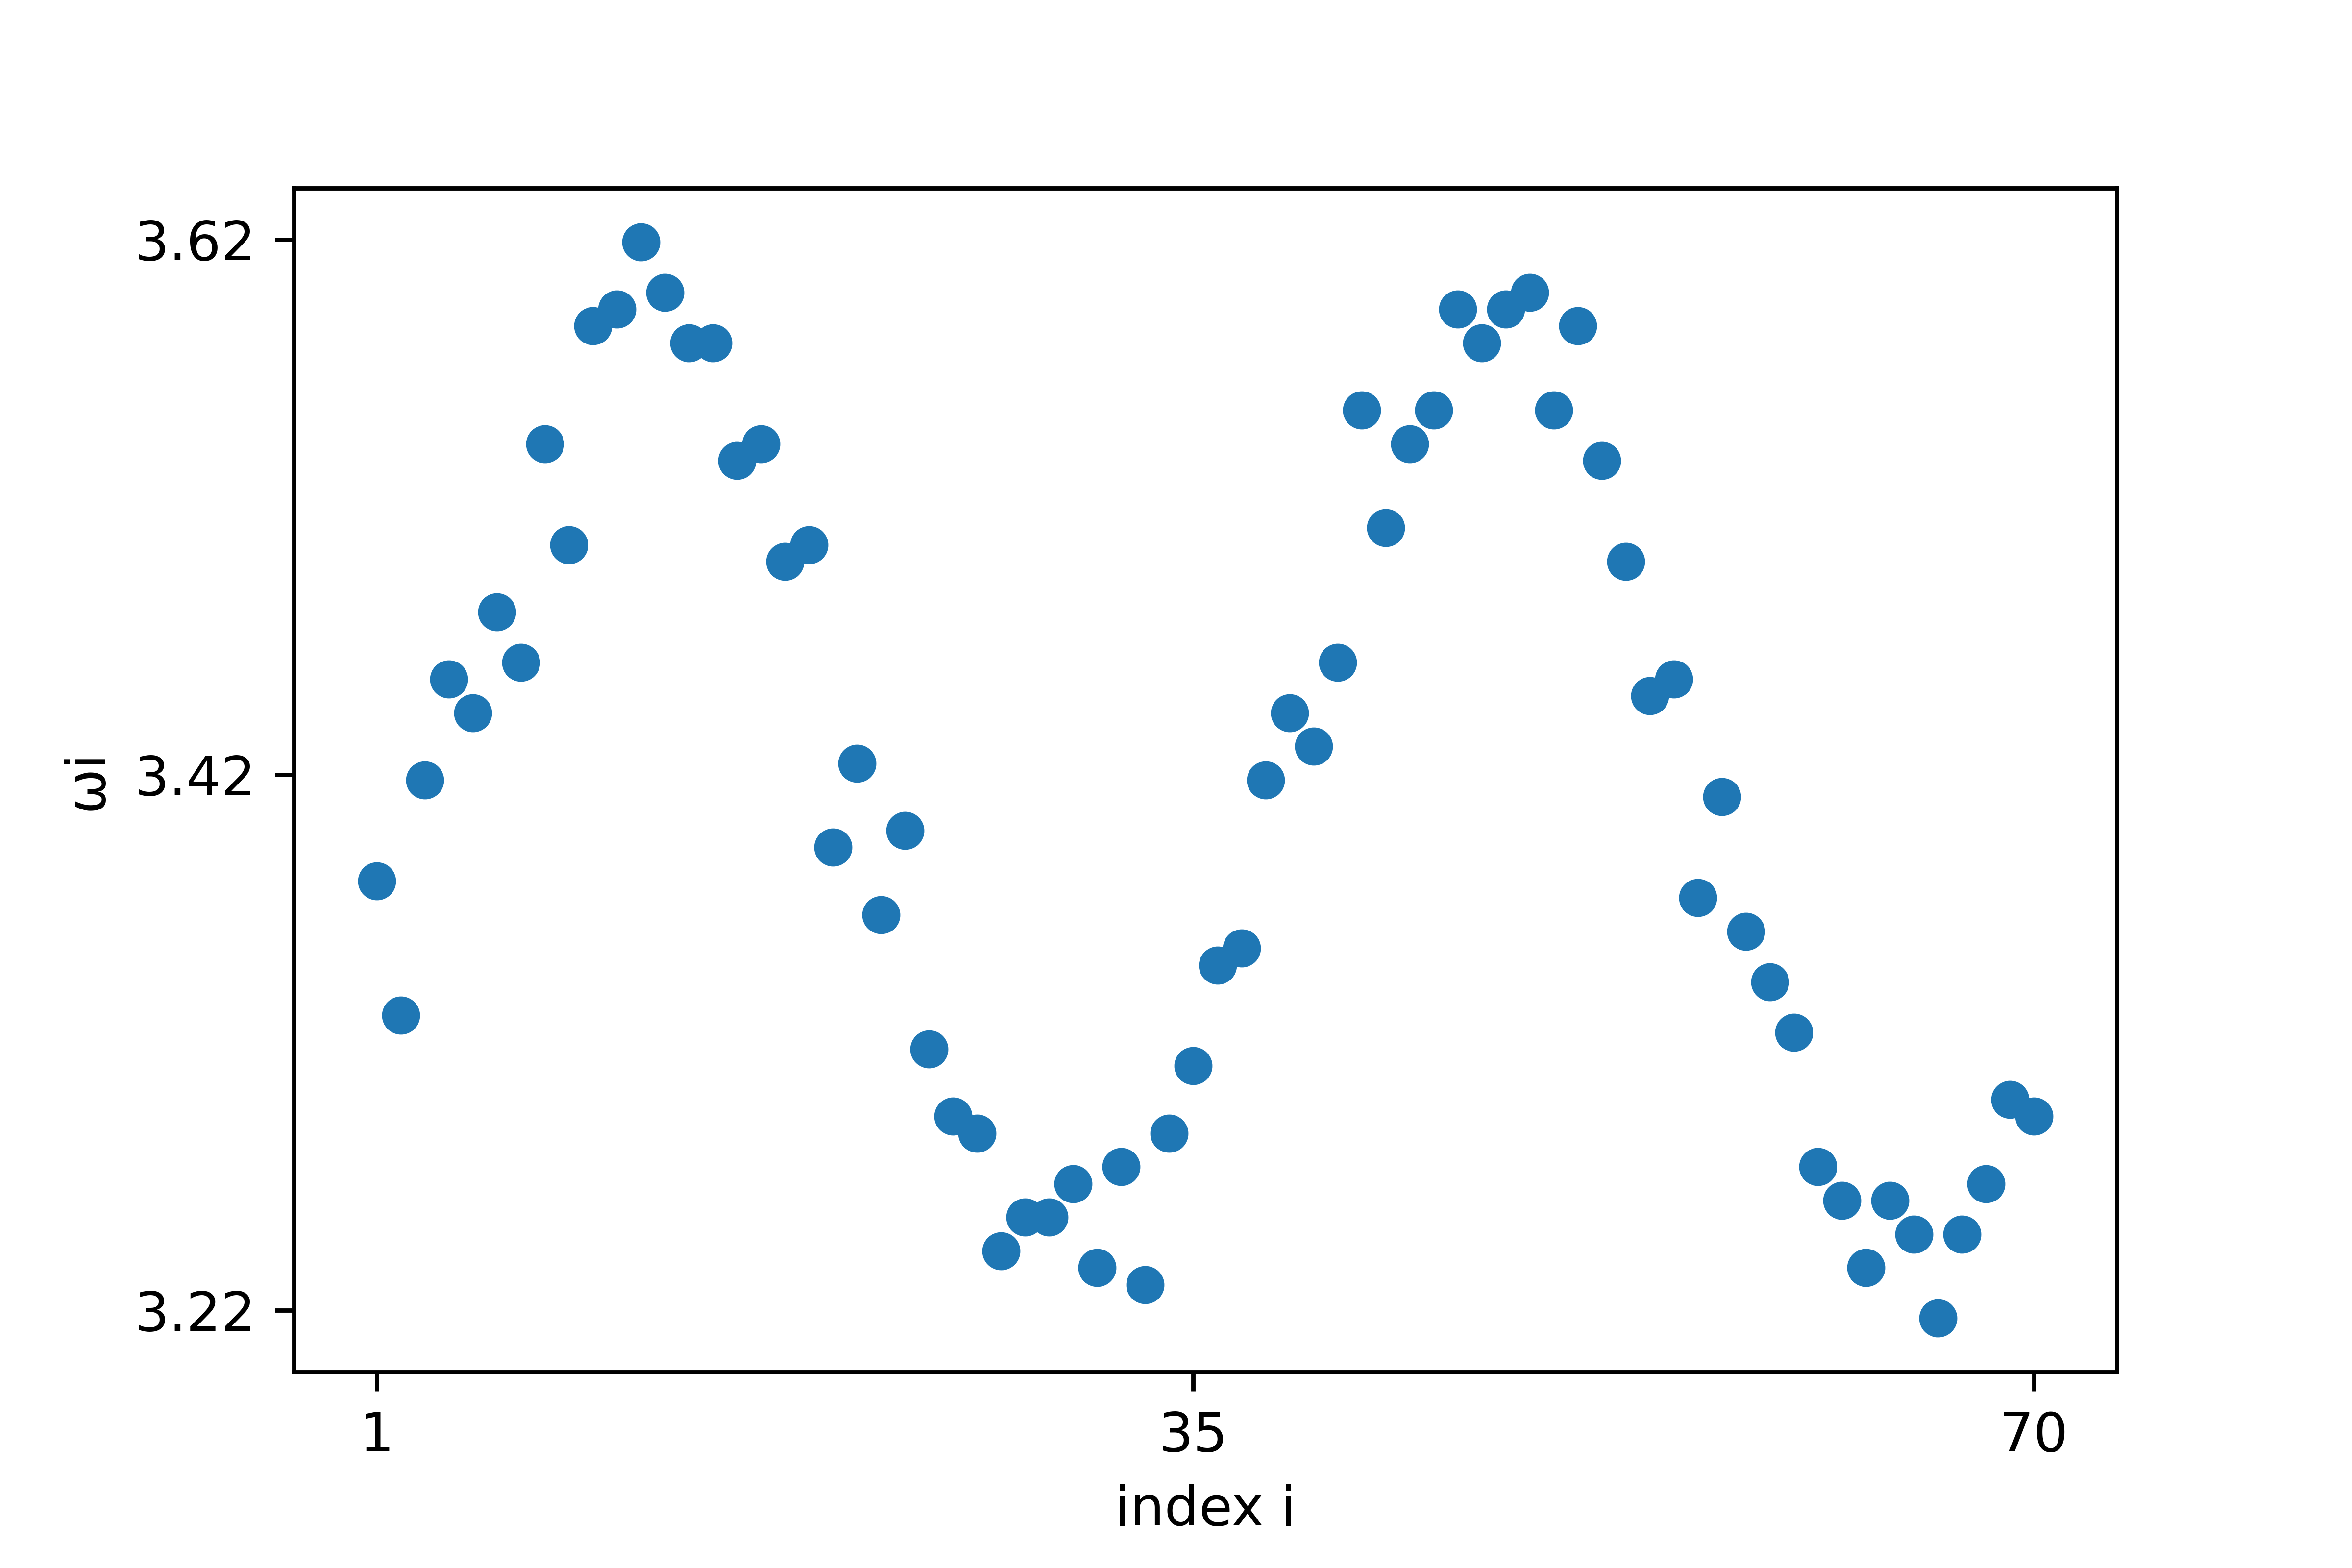
\includegraphics[width=1\linewidth]{w_sigma=1.6.png}  
  \caption{$\sigma = 1.6$}
\end{subfigure}
\hfill
\begin{subfigure}{.32\textwidth}
  \centering
  % include first image
  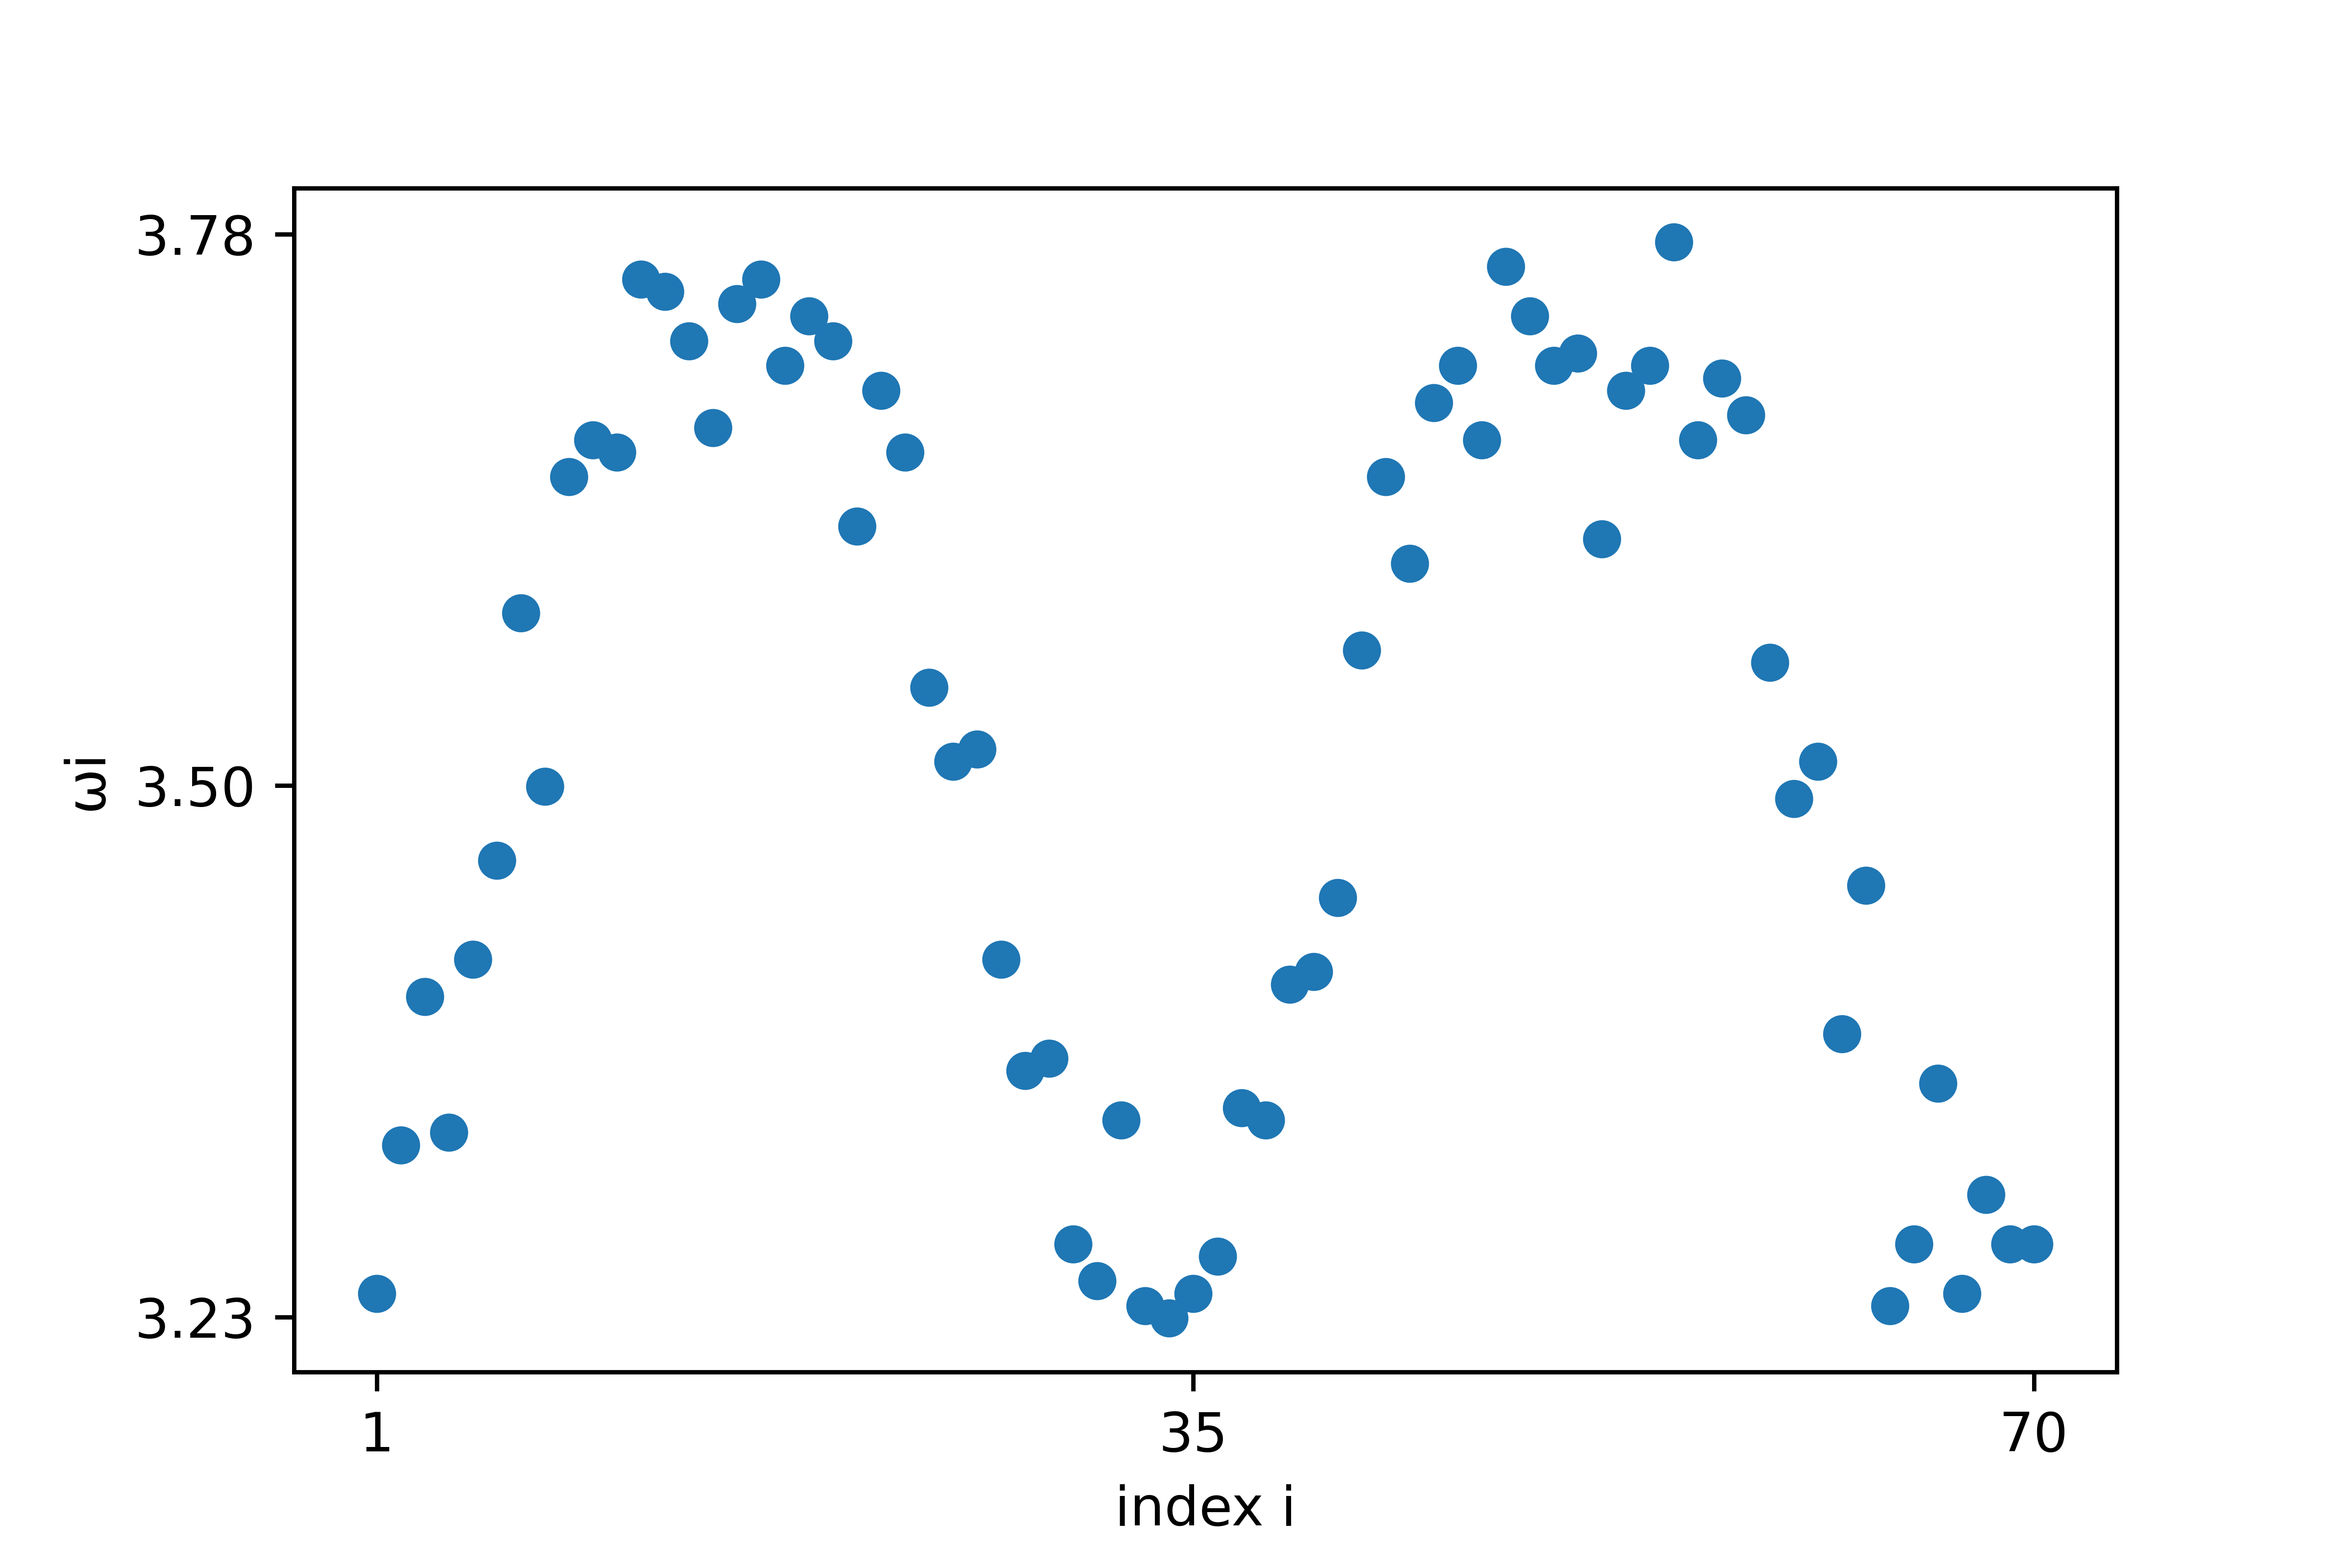
\includegraphics[width=1\linewidth]{w_sigma=1.7.png}  
  \caption{$\sigma = 1.7$}
\end{subfigure}
\caption{Snapshots of the membrane potential $u_i$ and mean phase-velocity profiles $\omega_i$ for the double chimeras observed, for $N=70$, $r=0.40$ at $t=1000$. The first row are the $u_i$ and the second row are the $\omega_i$.}
\label{dchim}
\end{figure}

\end{frame}

\begin{frame}{Varying $\sigma$}

\begin{figure}[H]
\centering
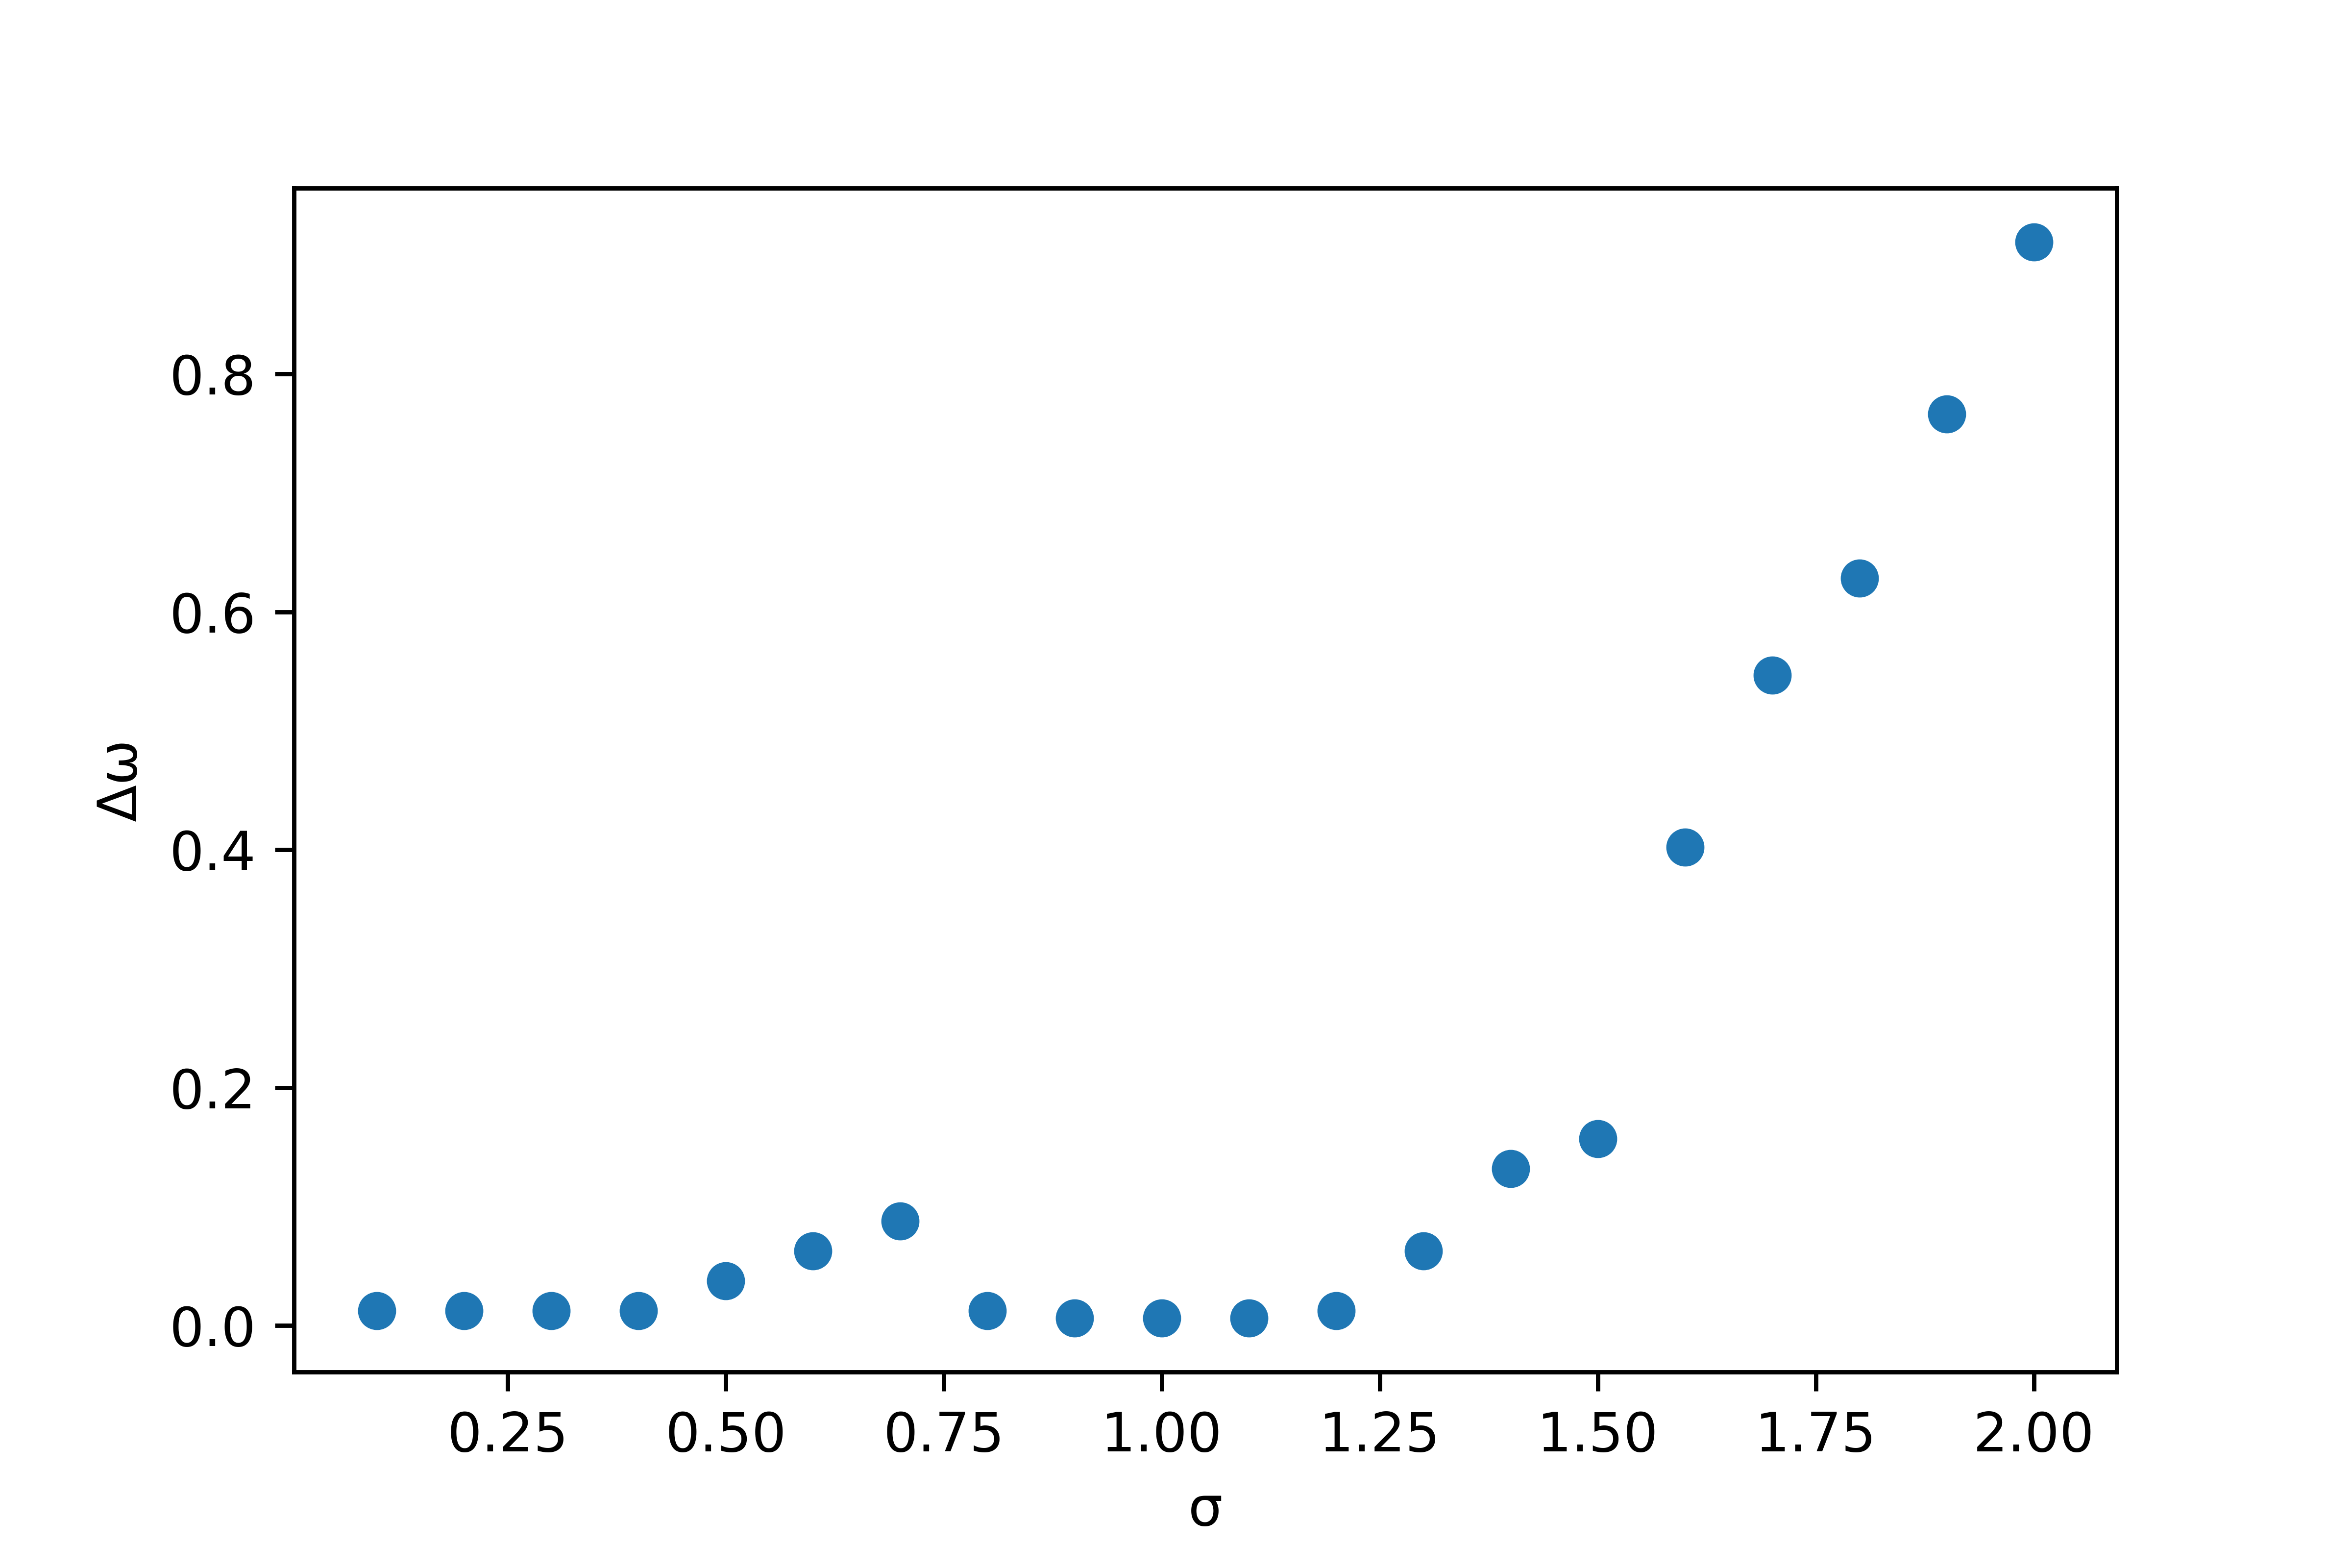
\includegraphics[width=0.6\textwidth]{deltaw.png}
\caption{$\Delta \omega = \omega_{\text{max}}-\omega_{\text{min}}$ with varying $\sigma$.}
\label{dchim2}
\end{figure}
\end{frame}

\subsection{Dependence on initial conditions}
\begin{frame}{Dependence on initial conditions} \pause

\begin{figure}[H]
\begin{subfigure}{0.49 \textwidth}
\centering
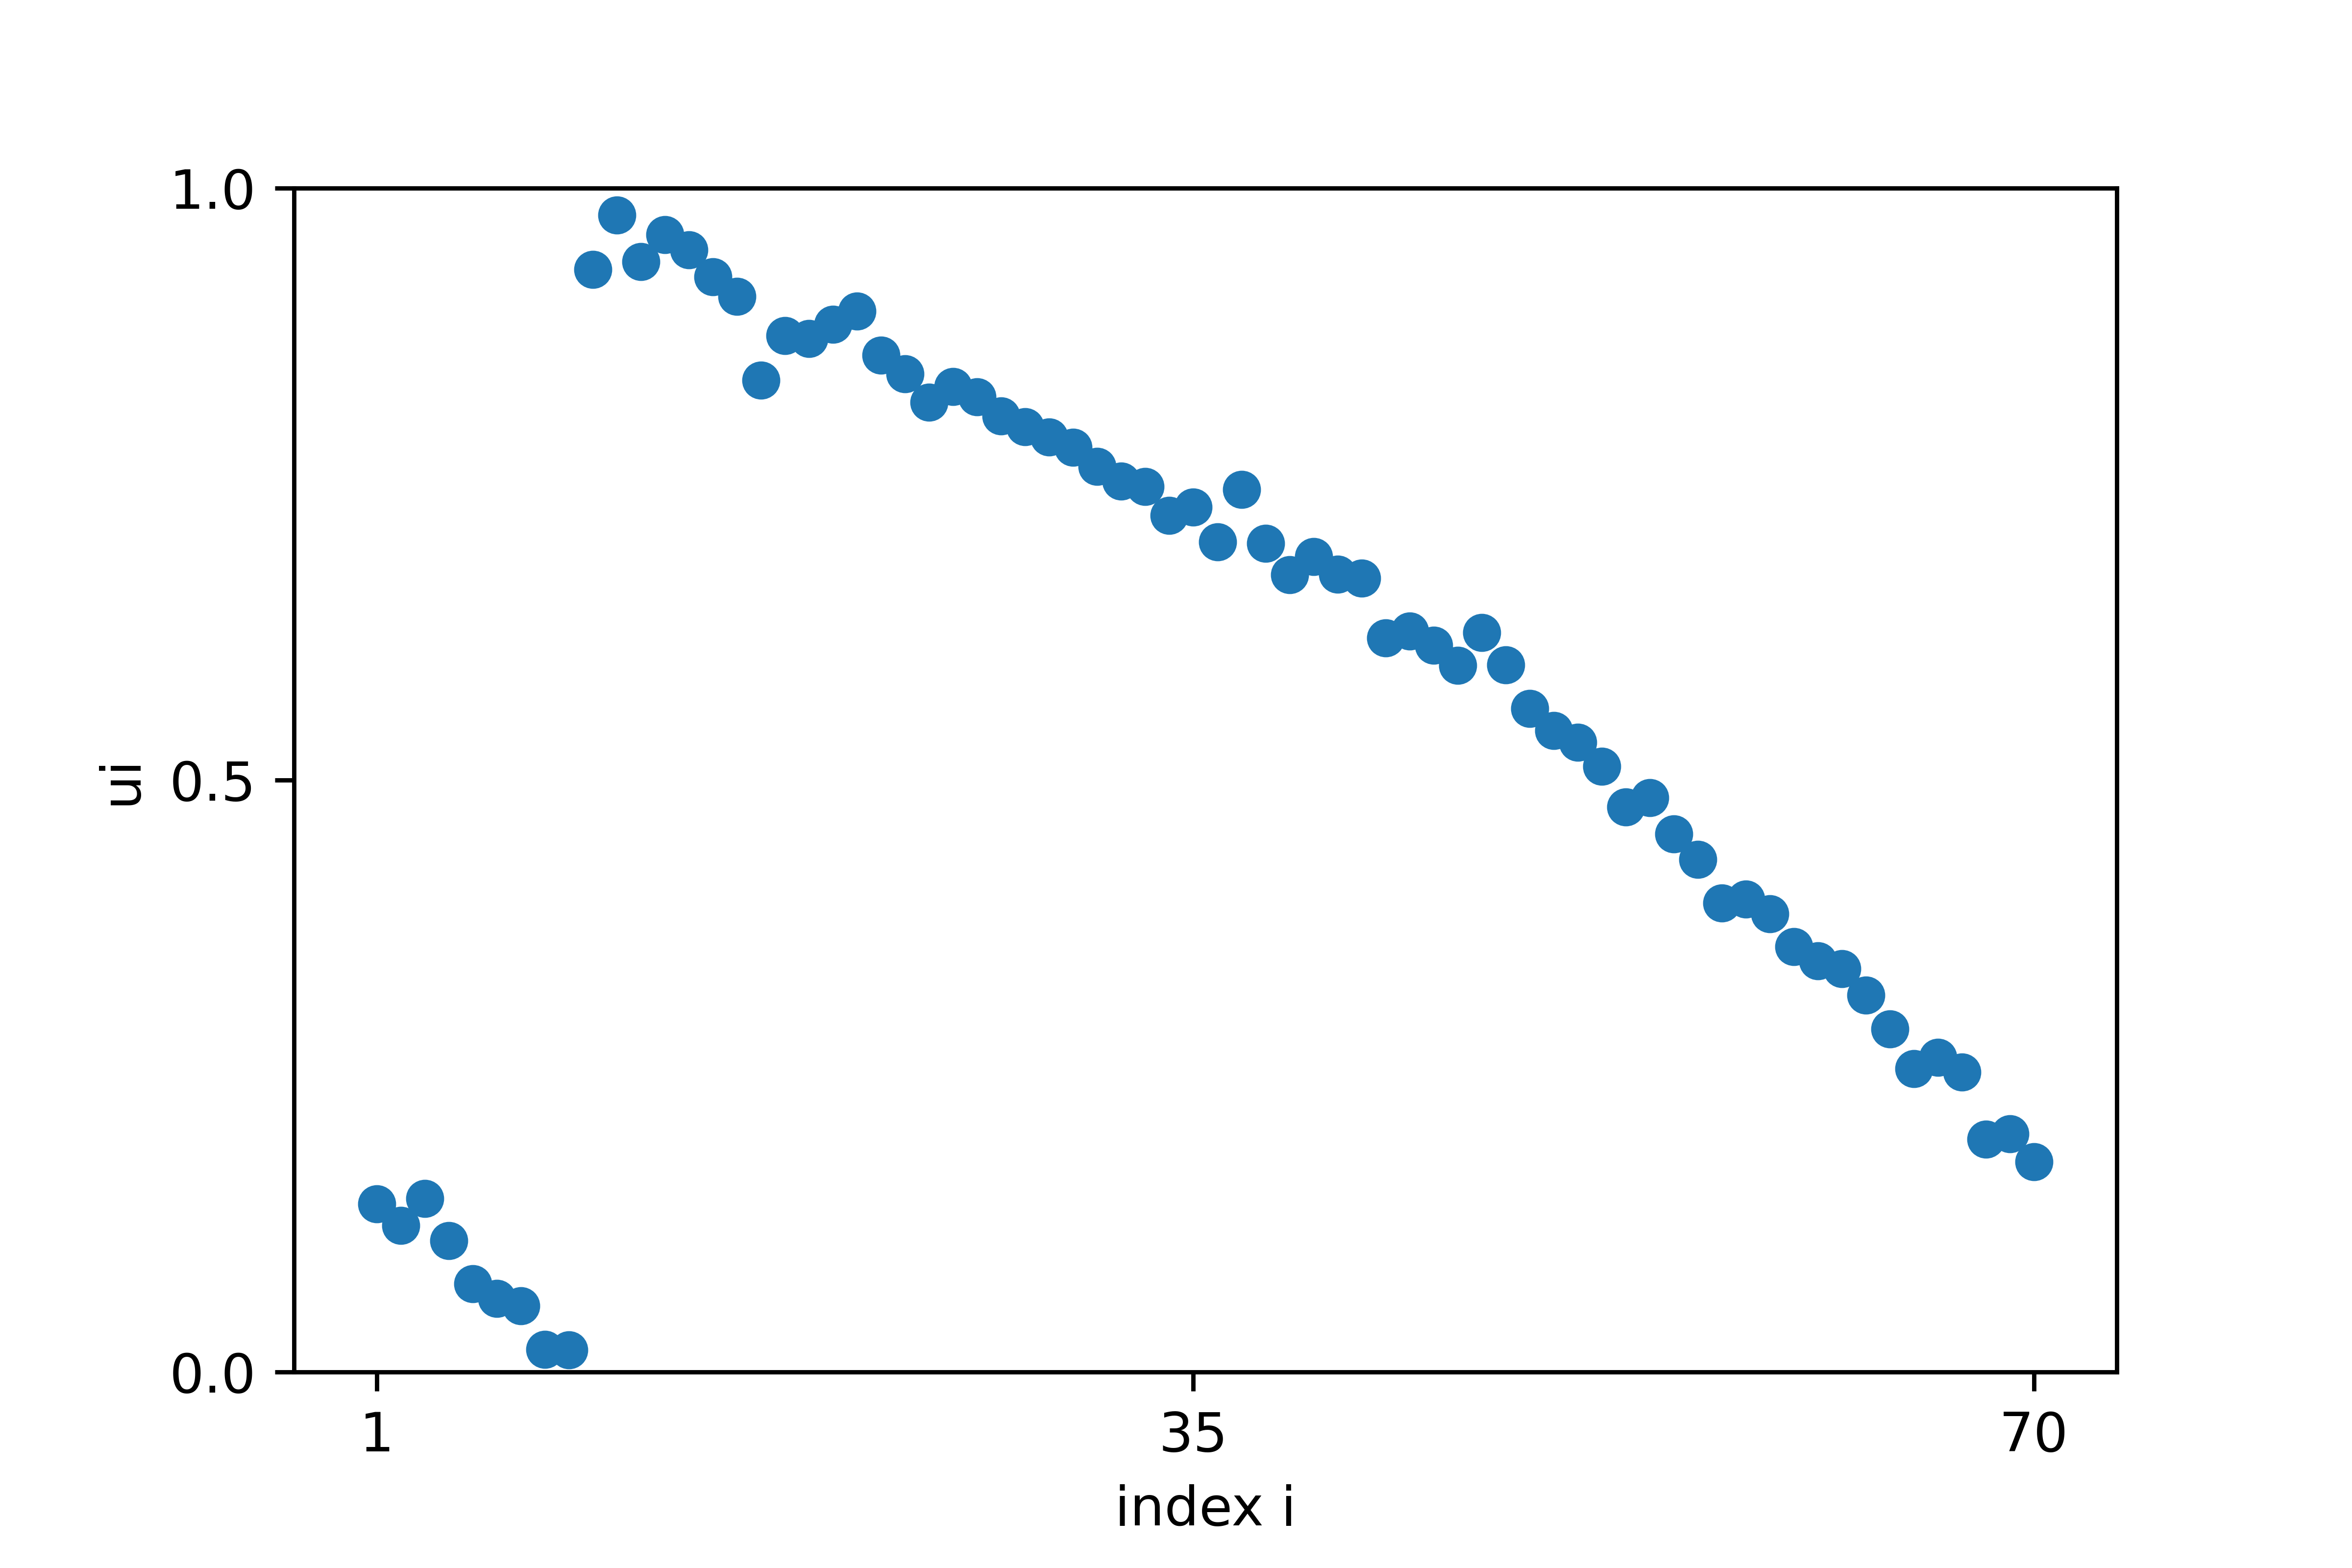
\includegraphics[width=\linewidth]{u_seed=64856_t=1000.png}
\caption{seed = $64856$}
\label{chain}
\end{subfigure}
\hfill
\begin{subfigure}{0.49 \textwidth}
\centering
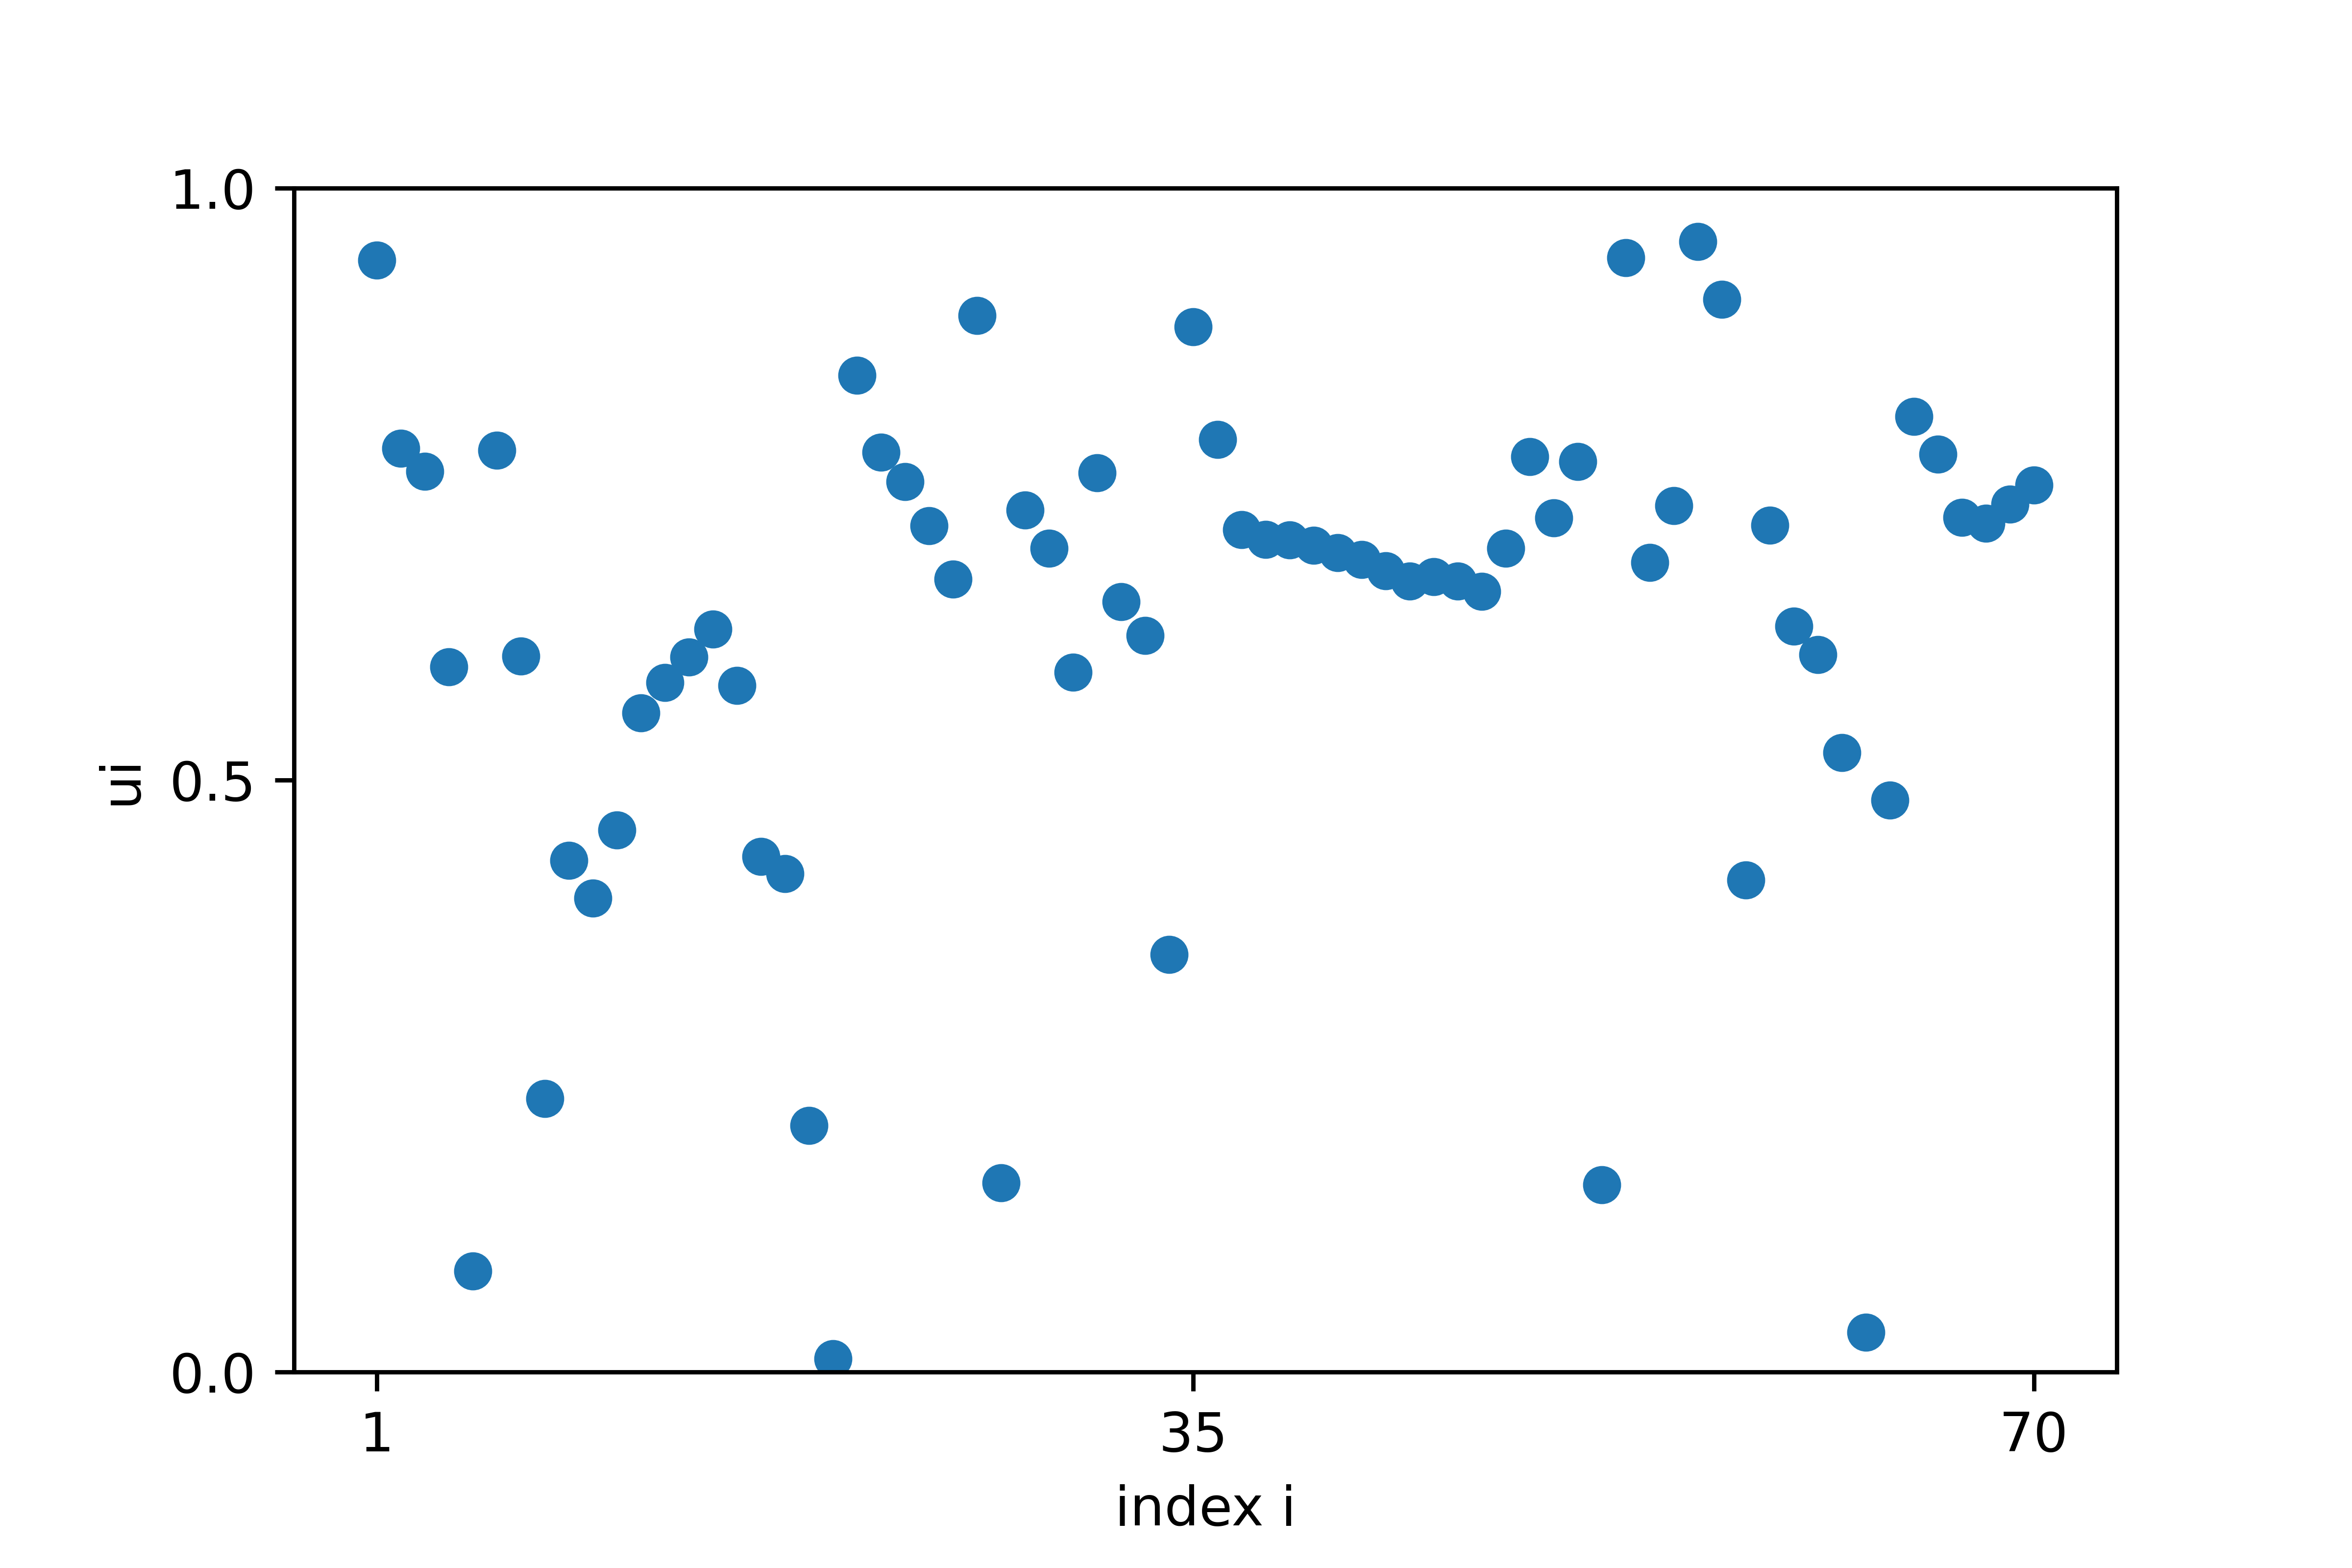
\includegraphics[width=\linewidth]{u_seed=38958_t=1000.png}
\caption{seed = $38958$} 
\label{chim}
\end{subfigure}
\caption{Snapshots of the membrane potential $u_i$ at $t=1000$, for $N=70$, $\sigma=0.7$ and $r=0.35$, for two different initial conditions.}
\end{figure} 

\end{frame}

\begin{frame}{Dependence on initial conditions}
\begin{figure}[H]
\begin{subfigure}{0.49 \textwidth}
\centering
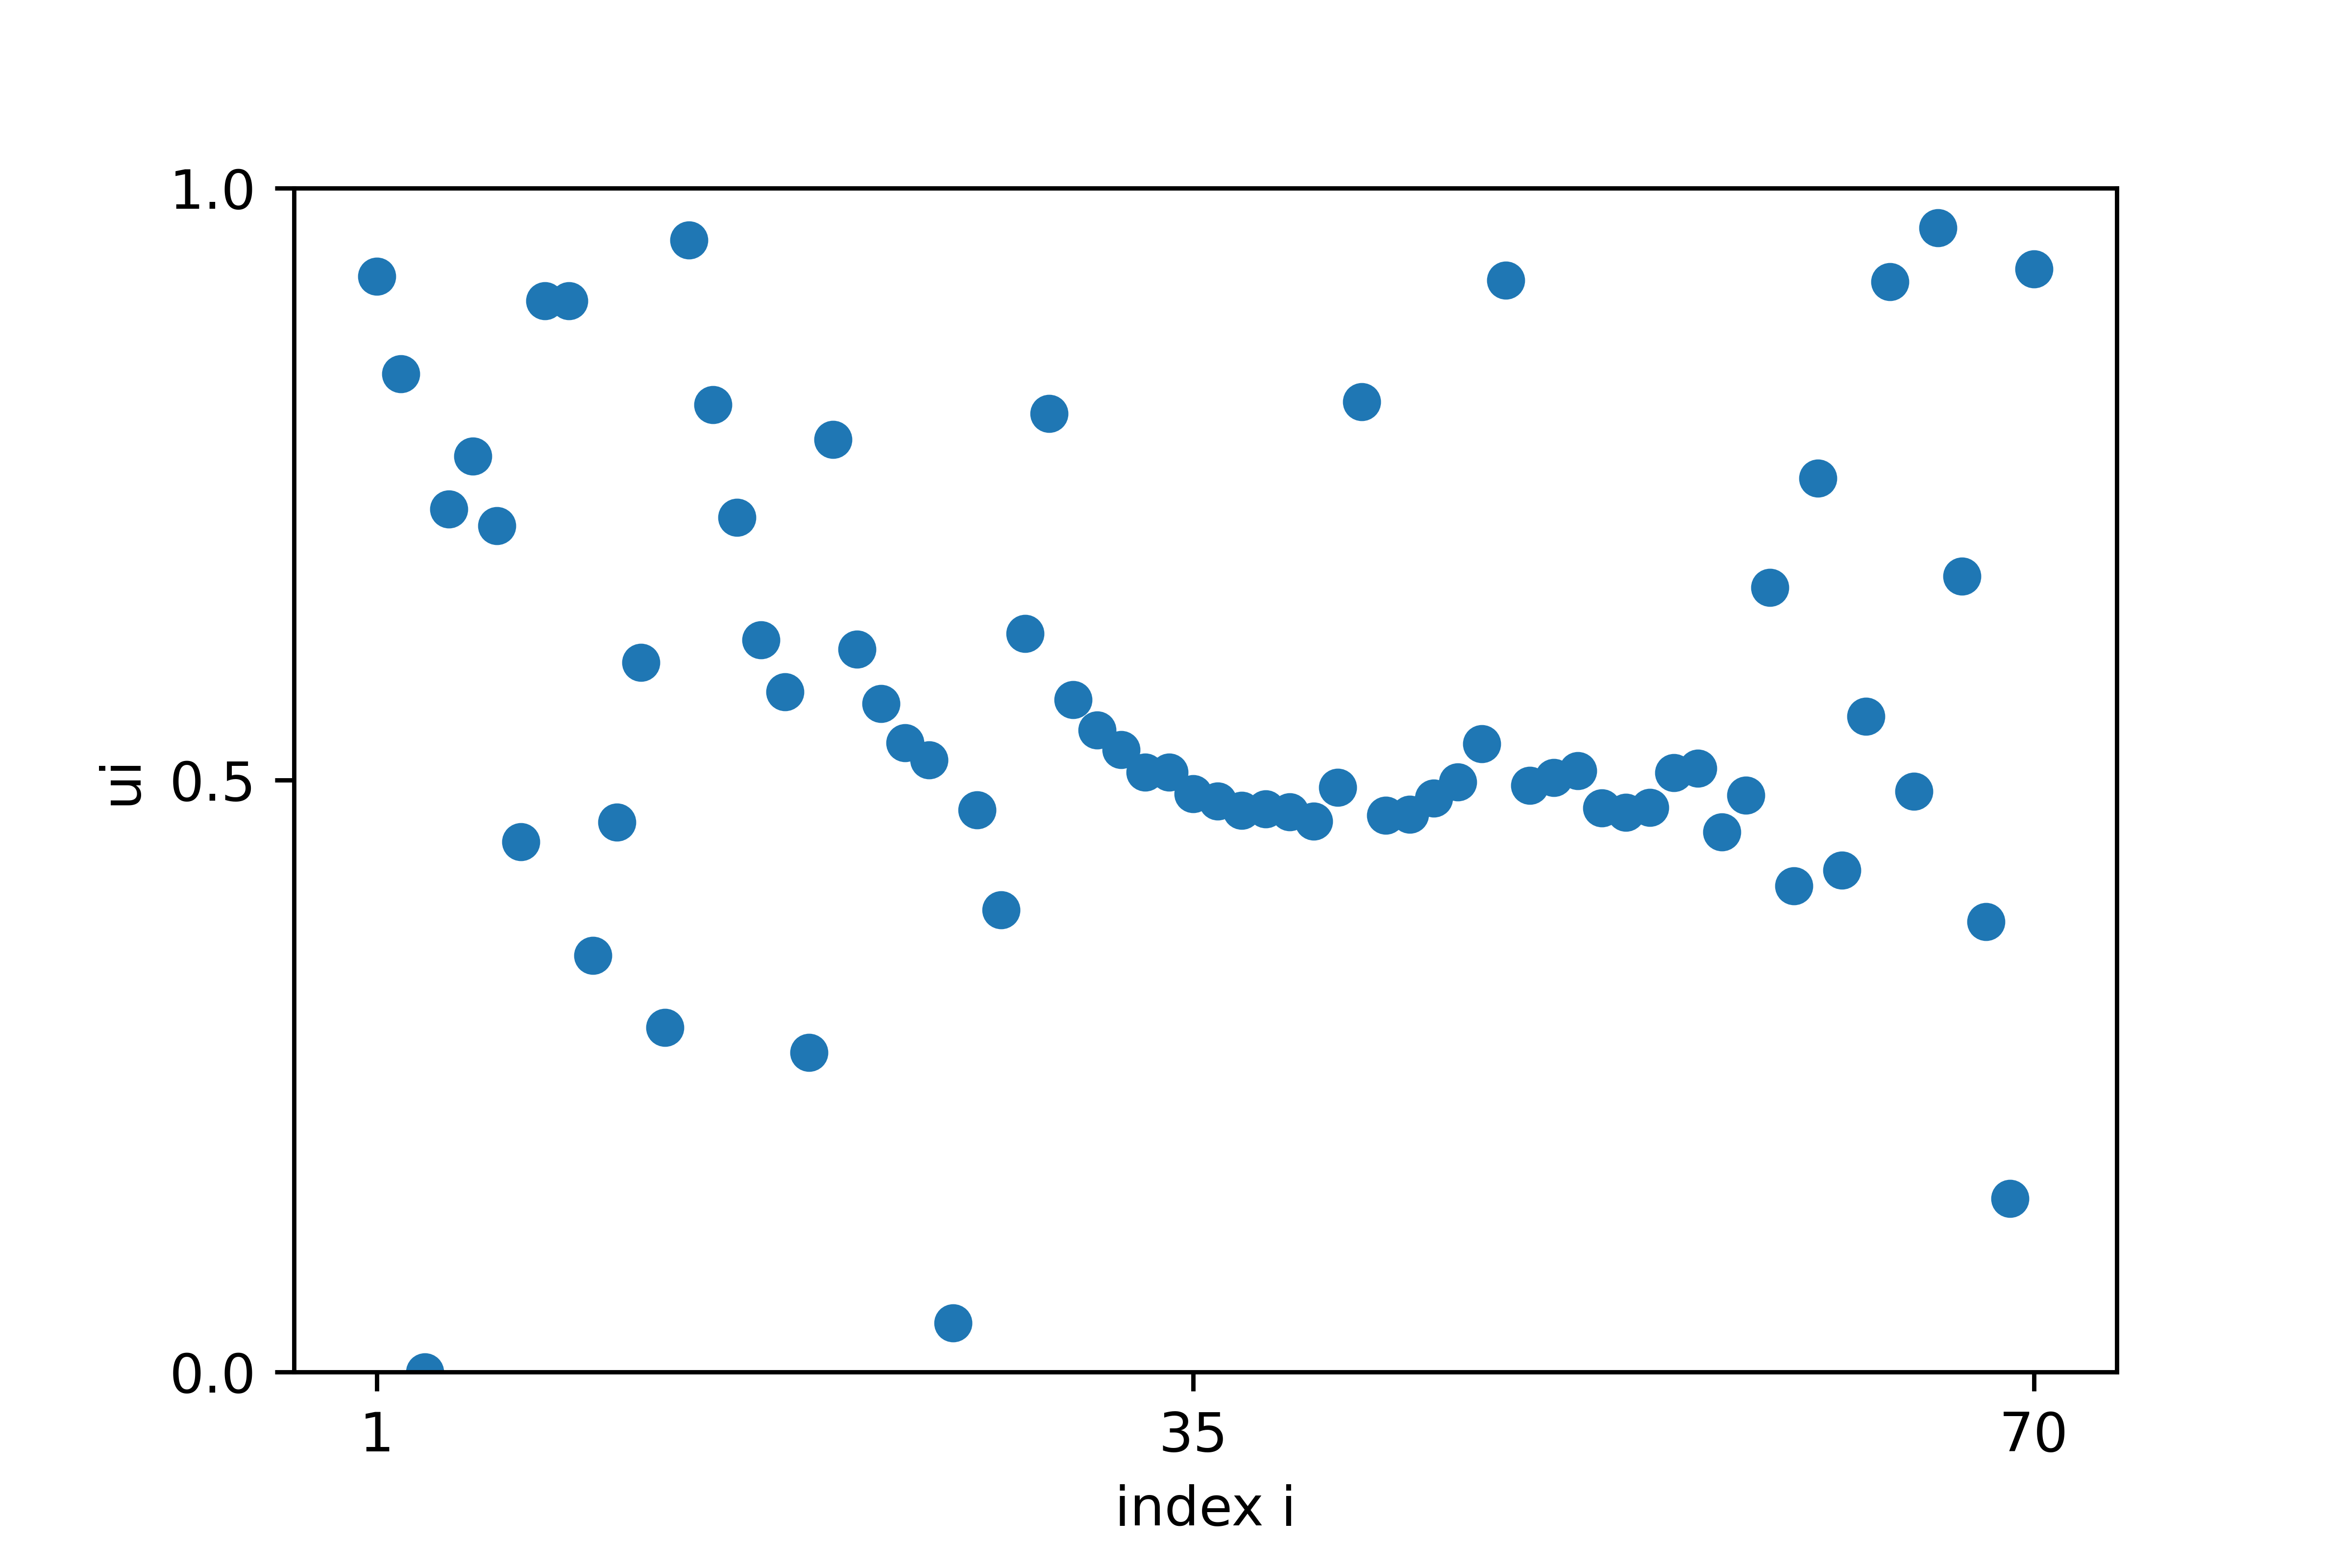
\includegraphics[width=\linewidth]{u_seed=70893_t=1000.png}
\caption{$t=1000$, seed = $70893$}

\end{subfigure}
\hfill
\begin{subfigure}{0.49 \textwidth}
\centering
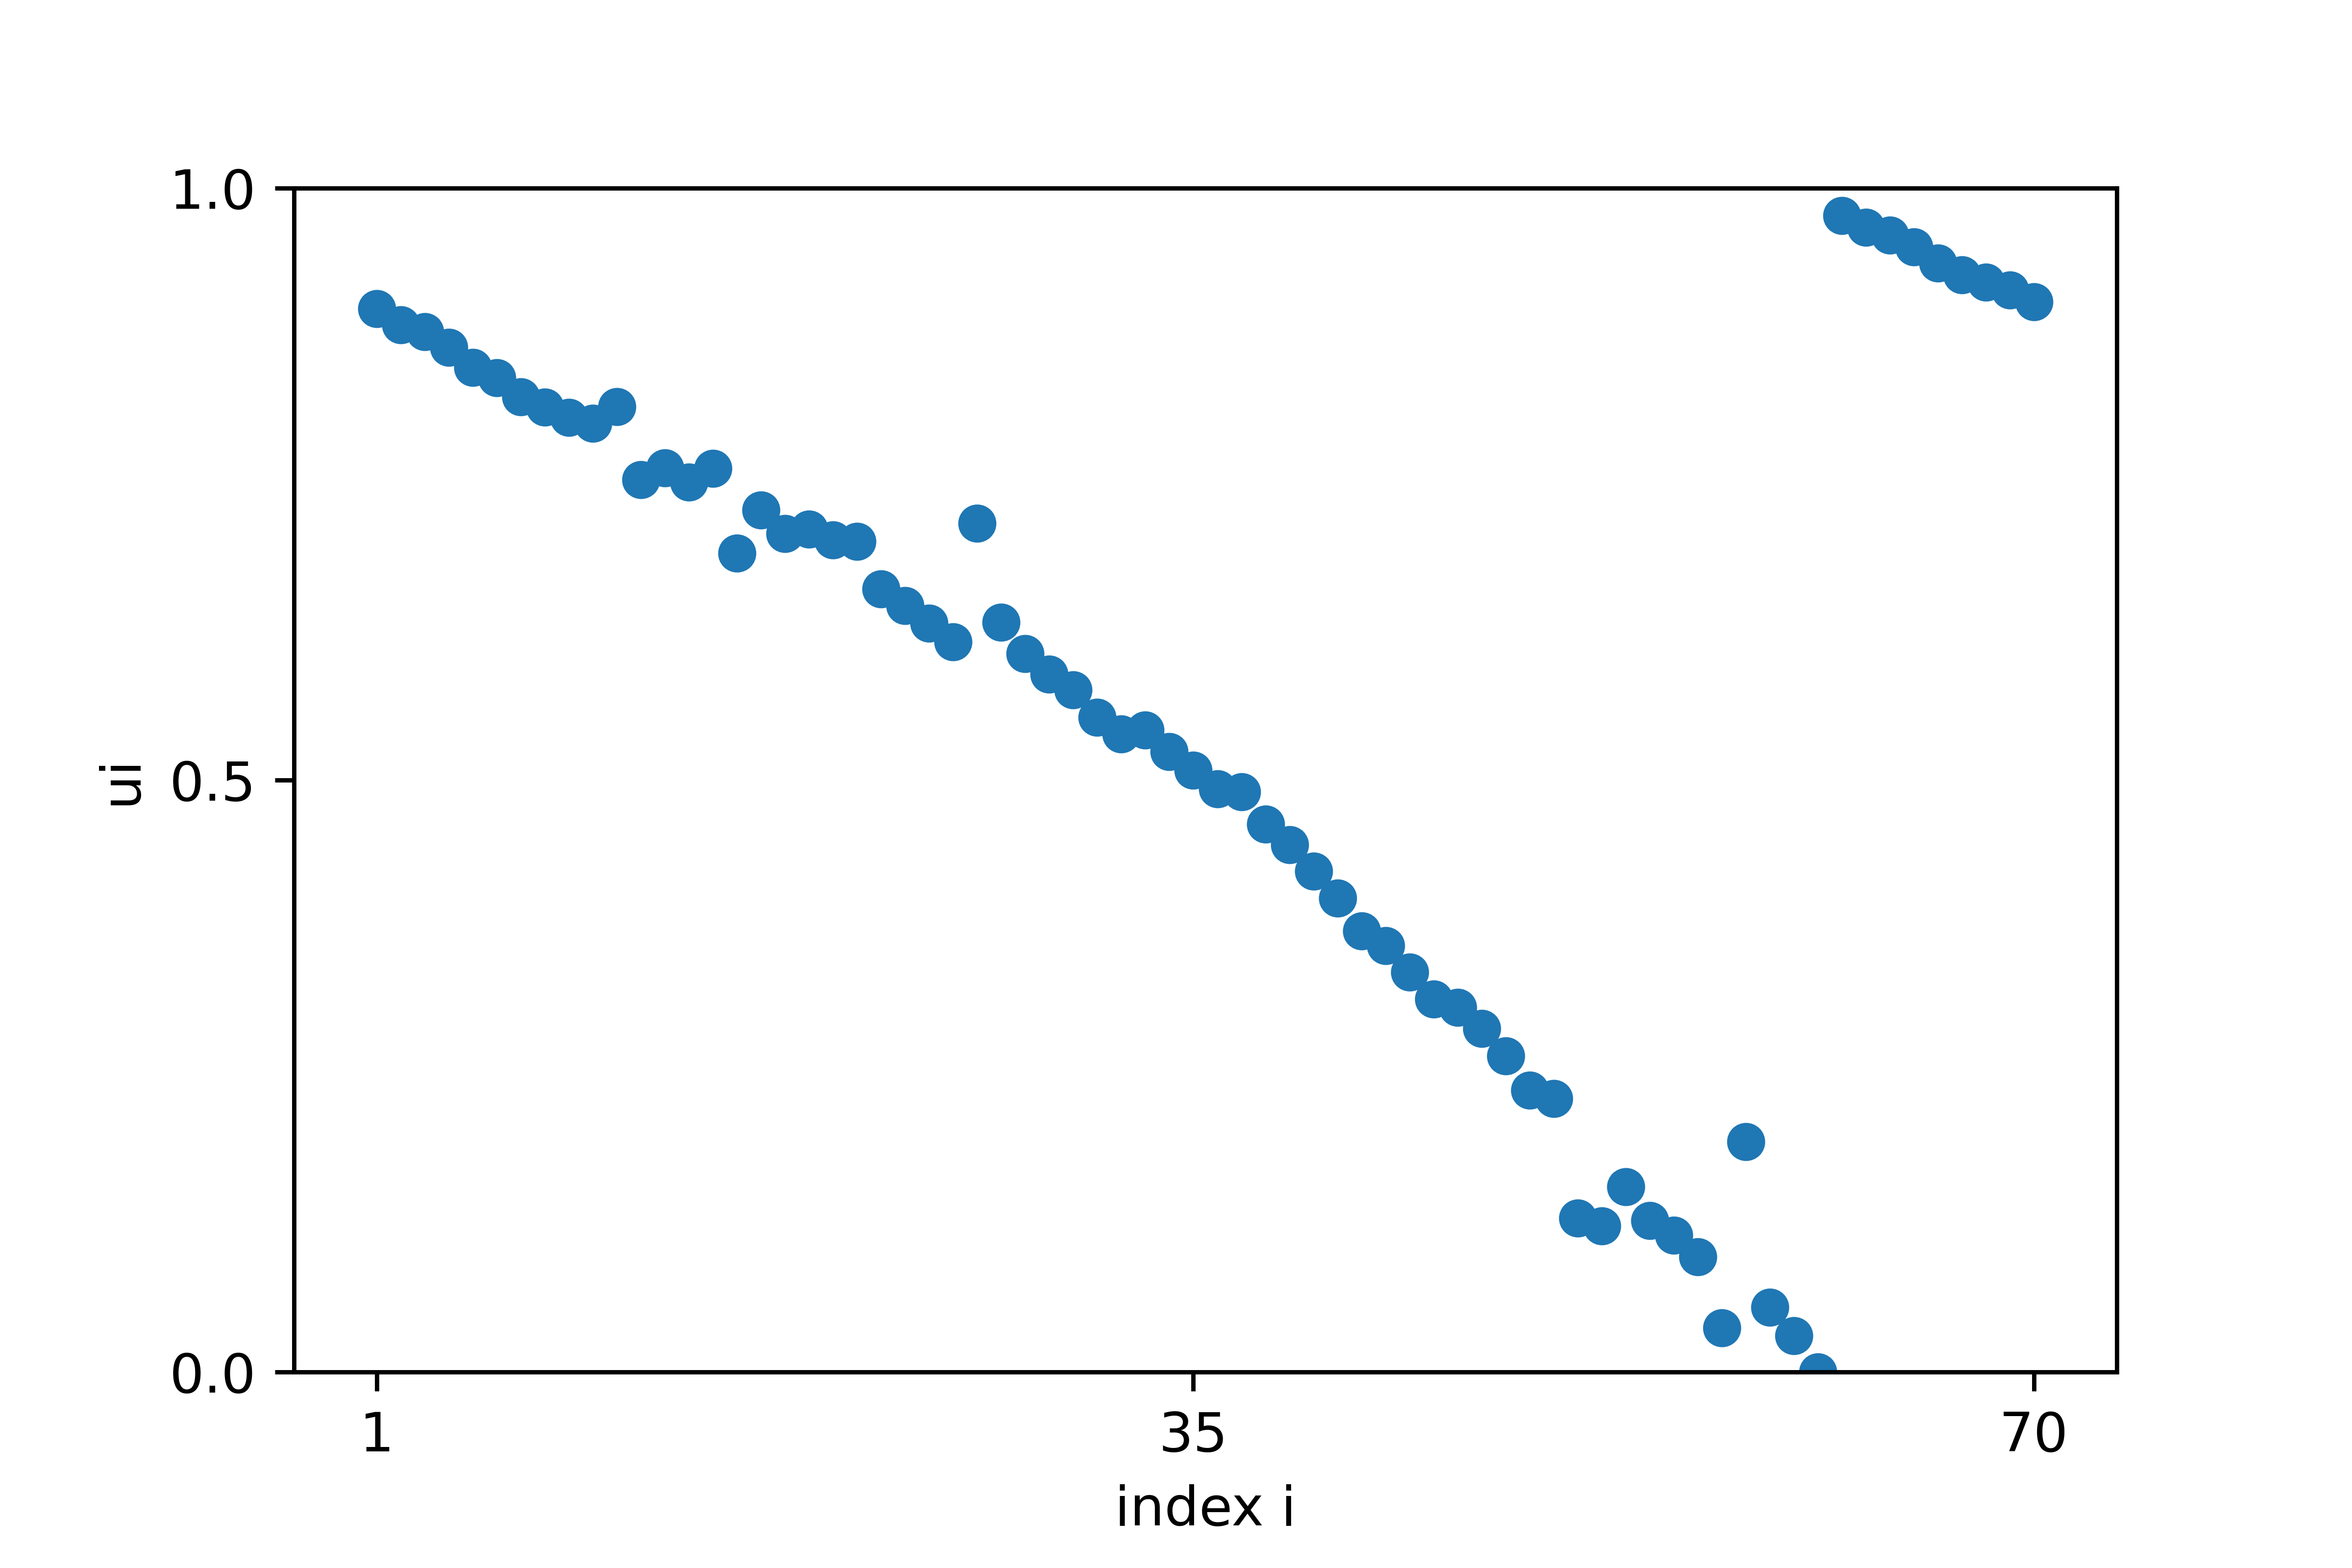
\includegraphics[width=\linewidth]{u_seed=70893_t=4000.png}
\caption{$t=4000$, seed = $70893$} 

\end{subfigure}
\caption{Snapshots of the membrane potential $u_i$, for $N=70$, $\sigma=0.7$ and $r=0.35$, at $t=1000$ and $t=4000$.}
\label{trans}
\end{figure} 
\end{frame}

\begin{frame}{Dependence on initial conditions}
\begin{figure}[H]
\begin{subfigure}{0.49 \textwidth}
\centering
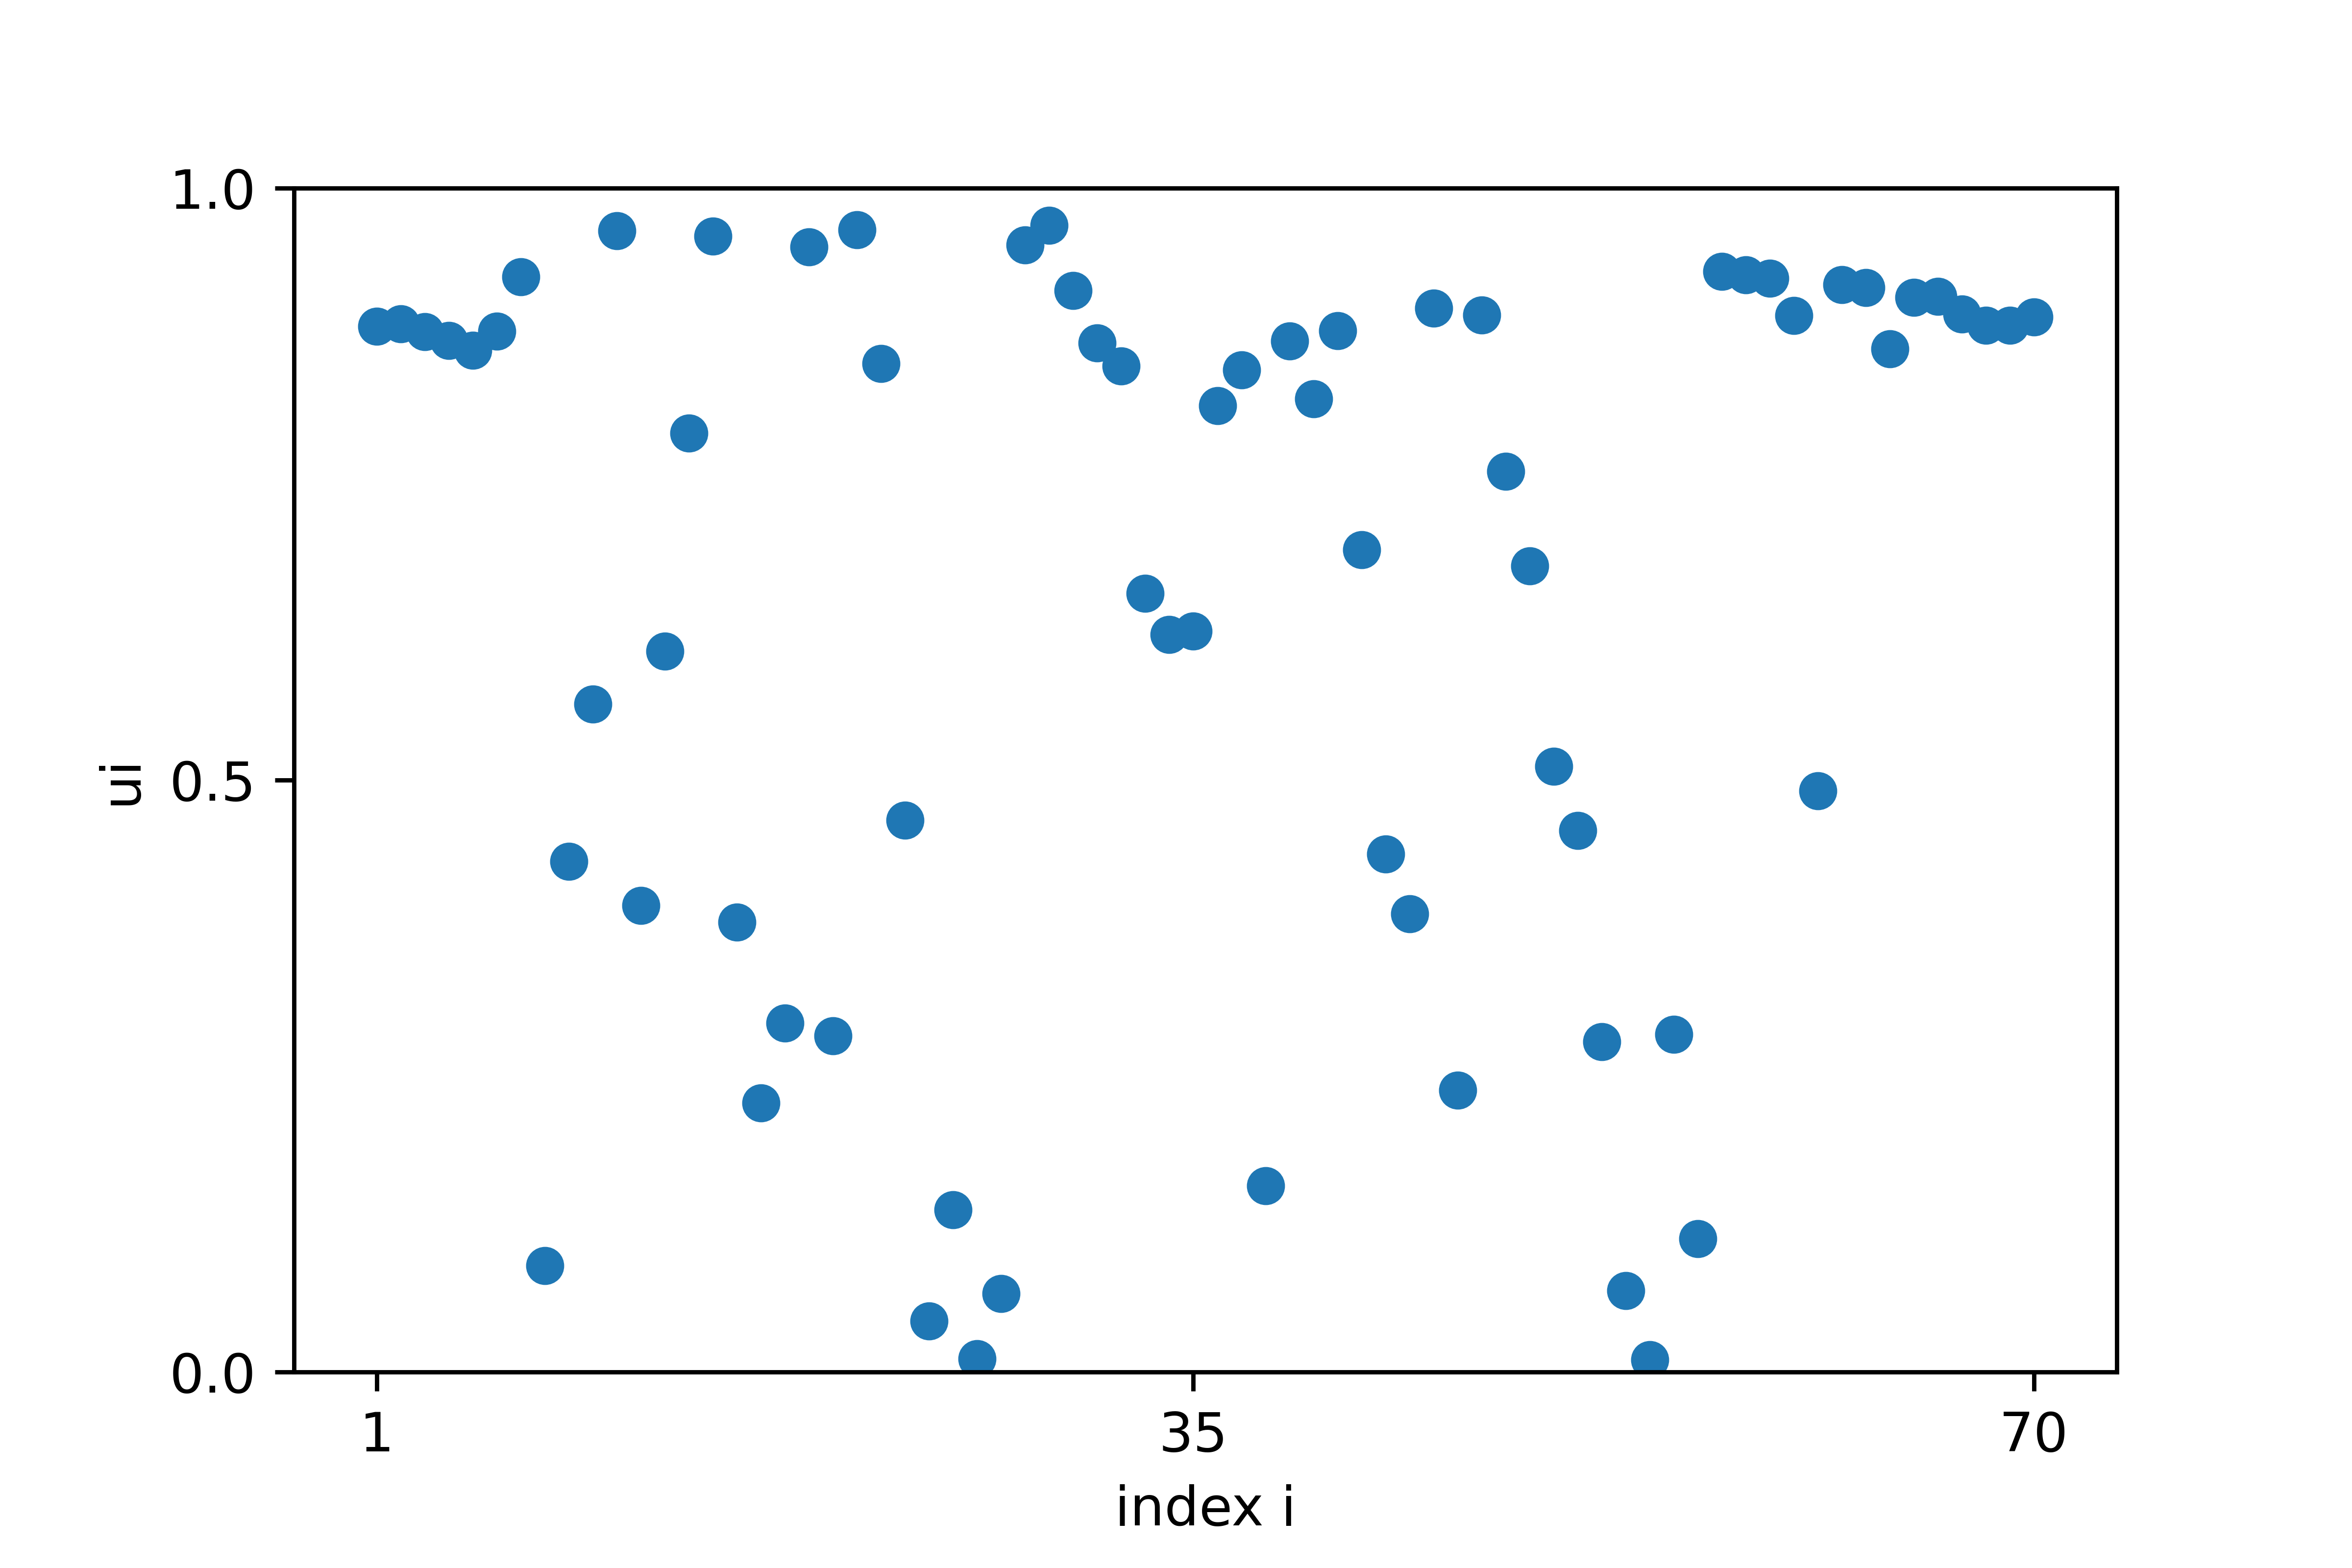
\includegraphics[width=\linewidth]{u_seed=27027_t=1000.png}
\caption{$t=1000$, seed = $27027$}
\end{subfigure}
\hfill
\begin{subfigure}{0.49 \textwidth}
\centering
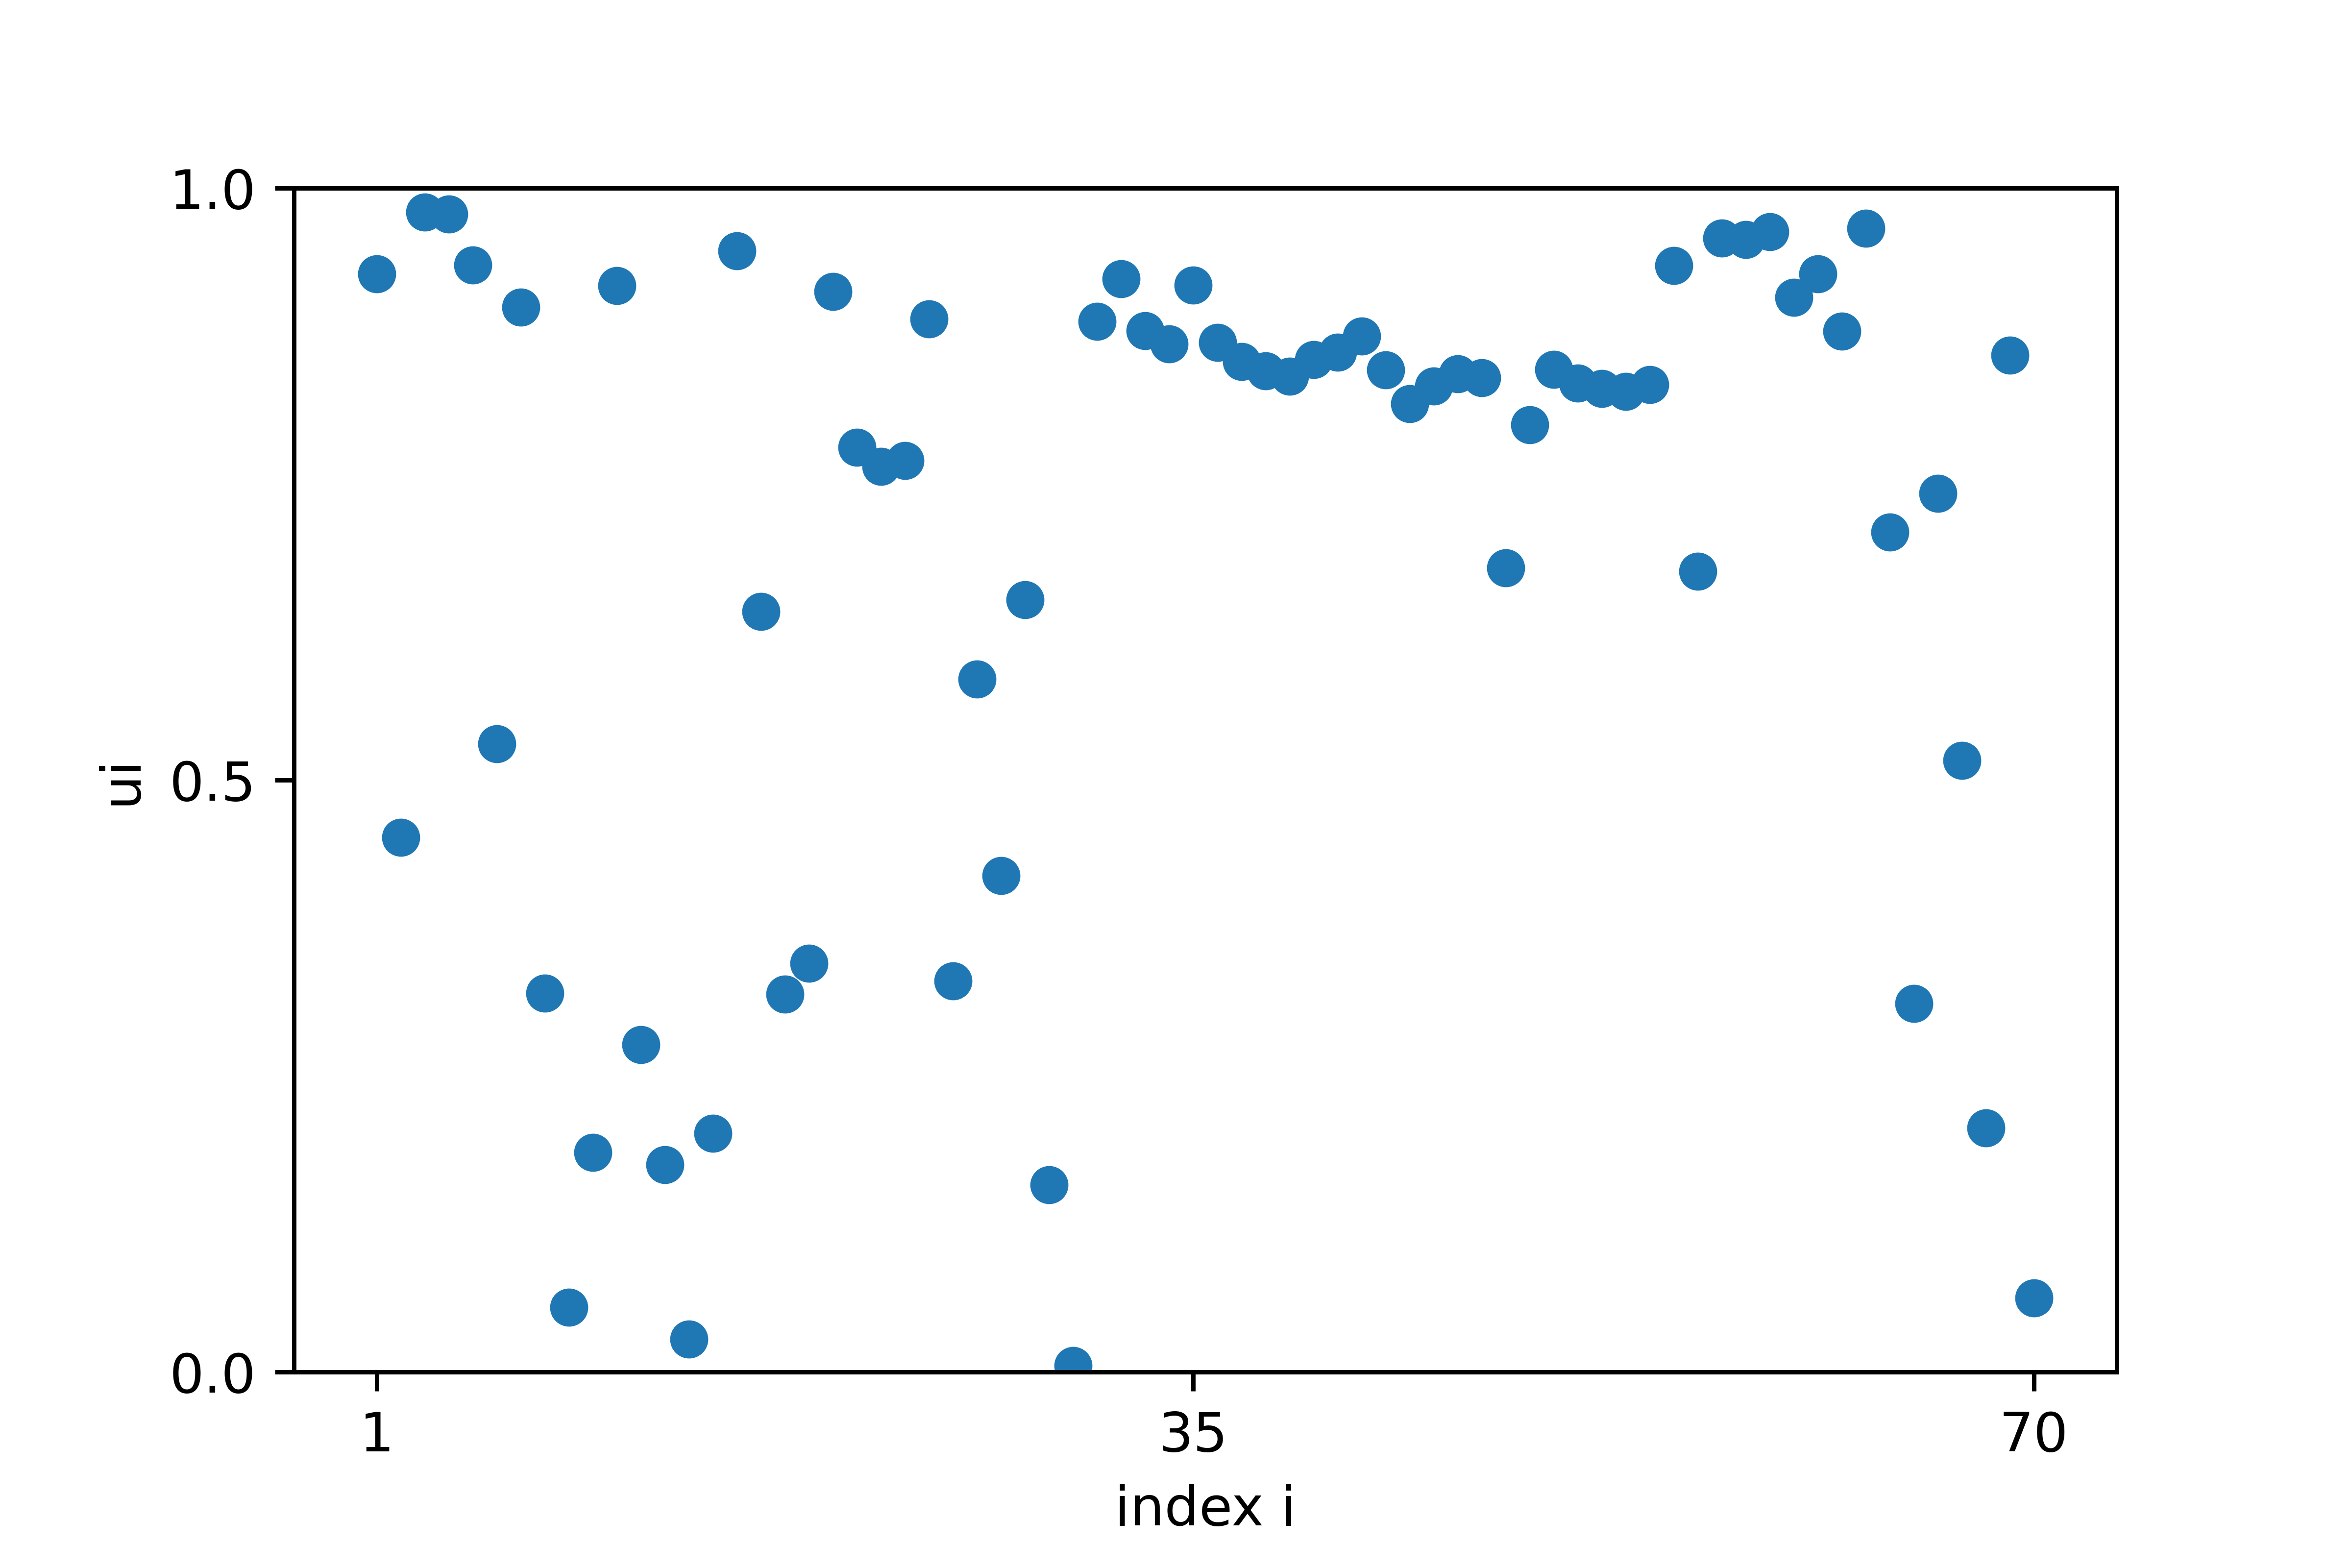
\includegraphics[width=\linewidth]{u_seed=27027_t=4000.png}
\caption{$t=4000$, seed = $27027$} 
\end{subfigure}
\caption{Snapshots of the membrane potential $u_i$ at $t=1000$ and $t=4000$, for $N=70$, $\sigma=0.7$ and $r=0.35$.}
\label{notrans}
\end{figure} 
\end{frame}

\section{The modified LIF model}
\subsection{Chimeras states in the non-leaky integrate-and-fire model}
\begin{frame}{Chimera states in the $\lambda = 0$ model} \pause

\begin{figure}[H]
\begin{subfigure}{0.49 \textwidth}
\centering
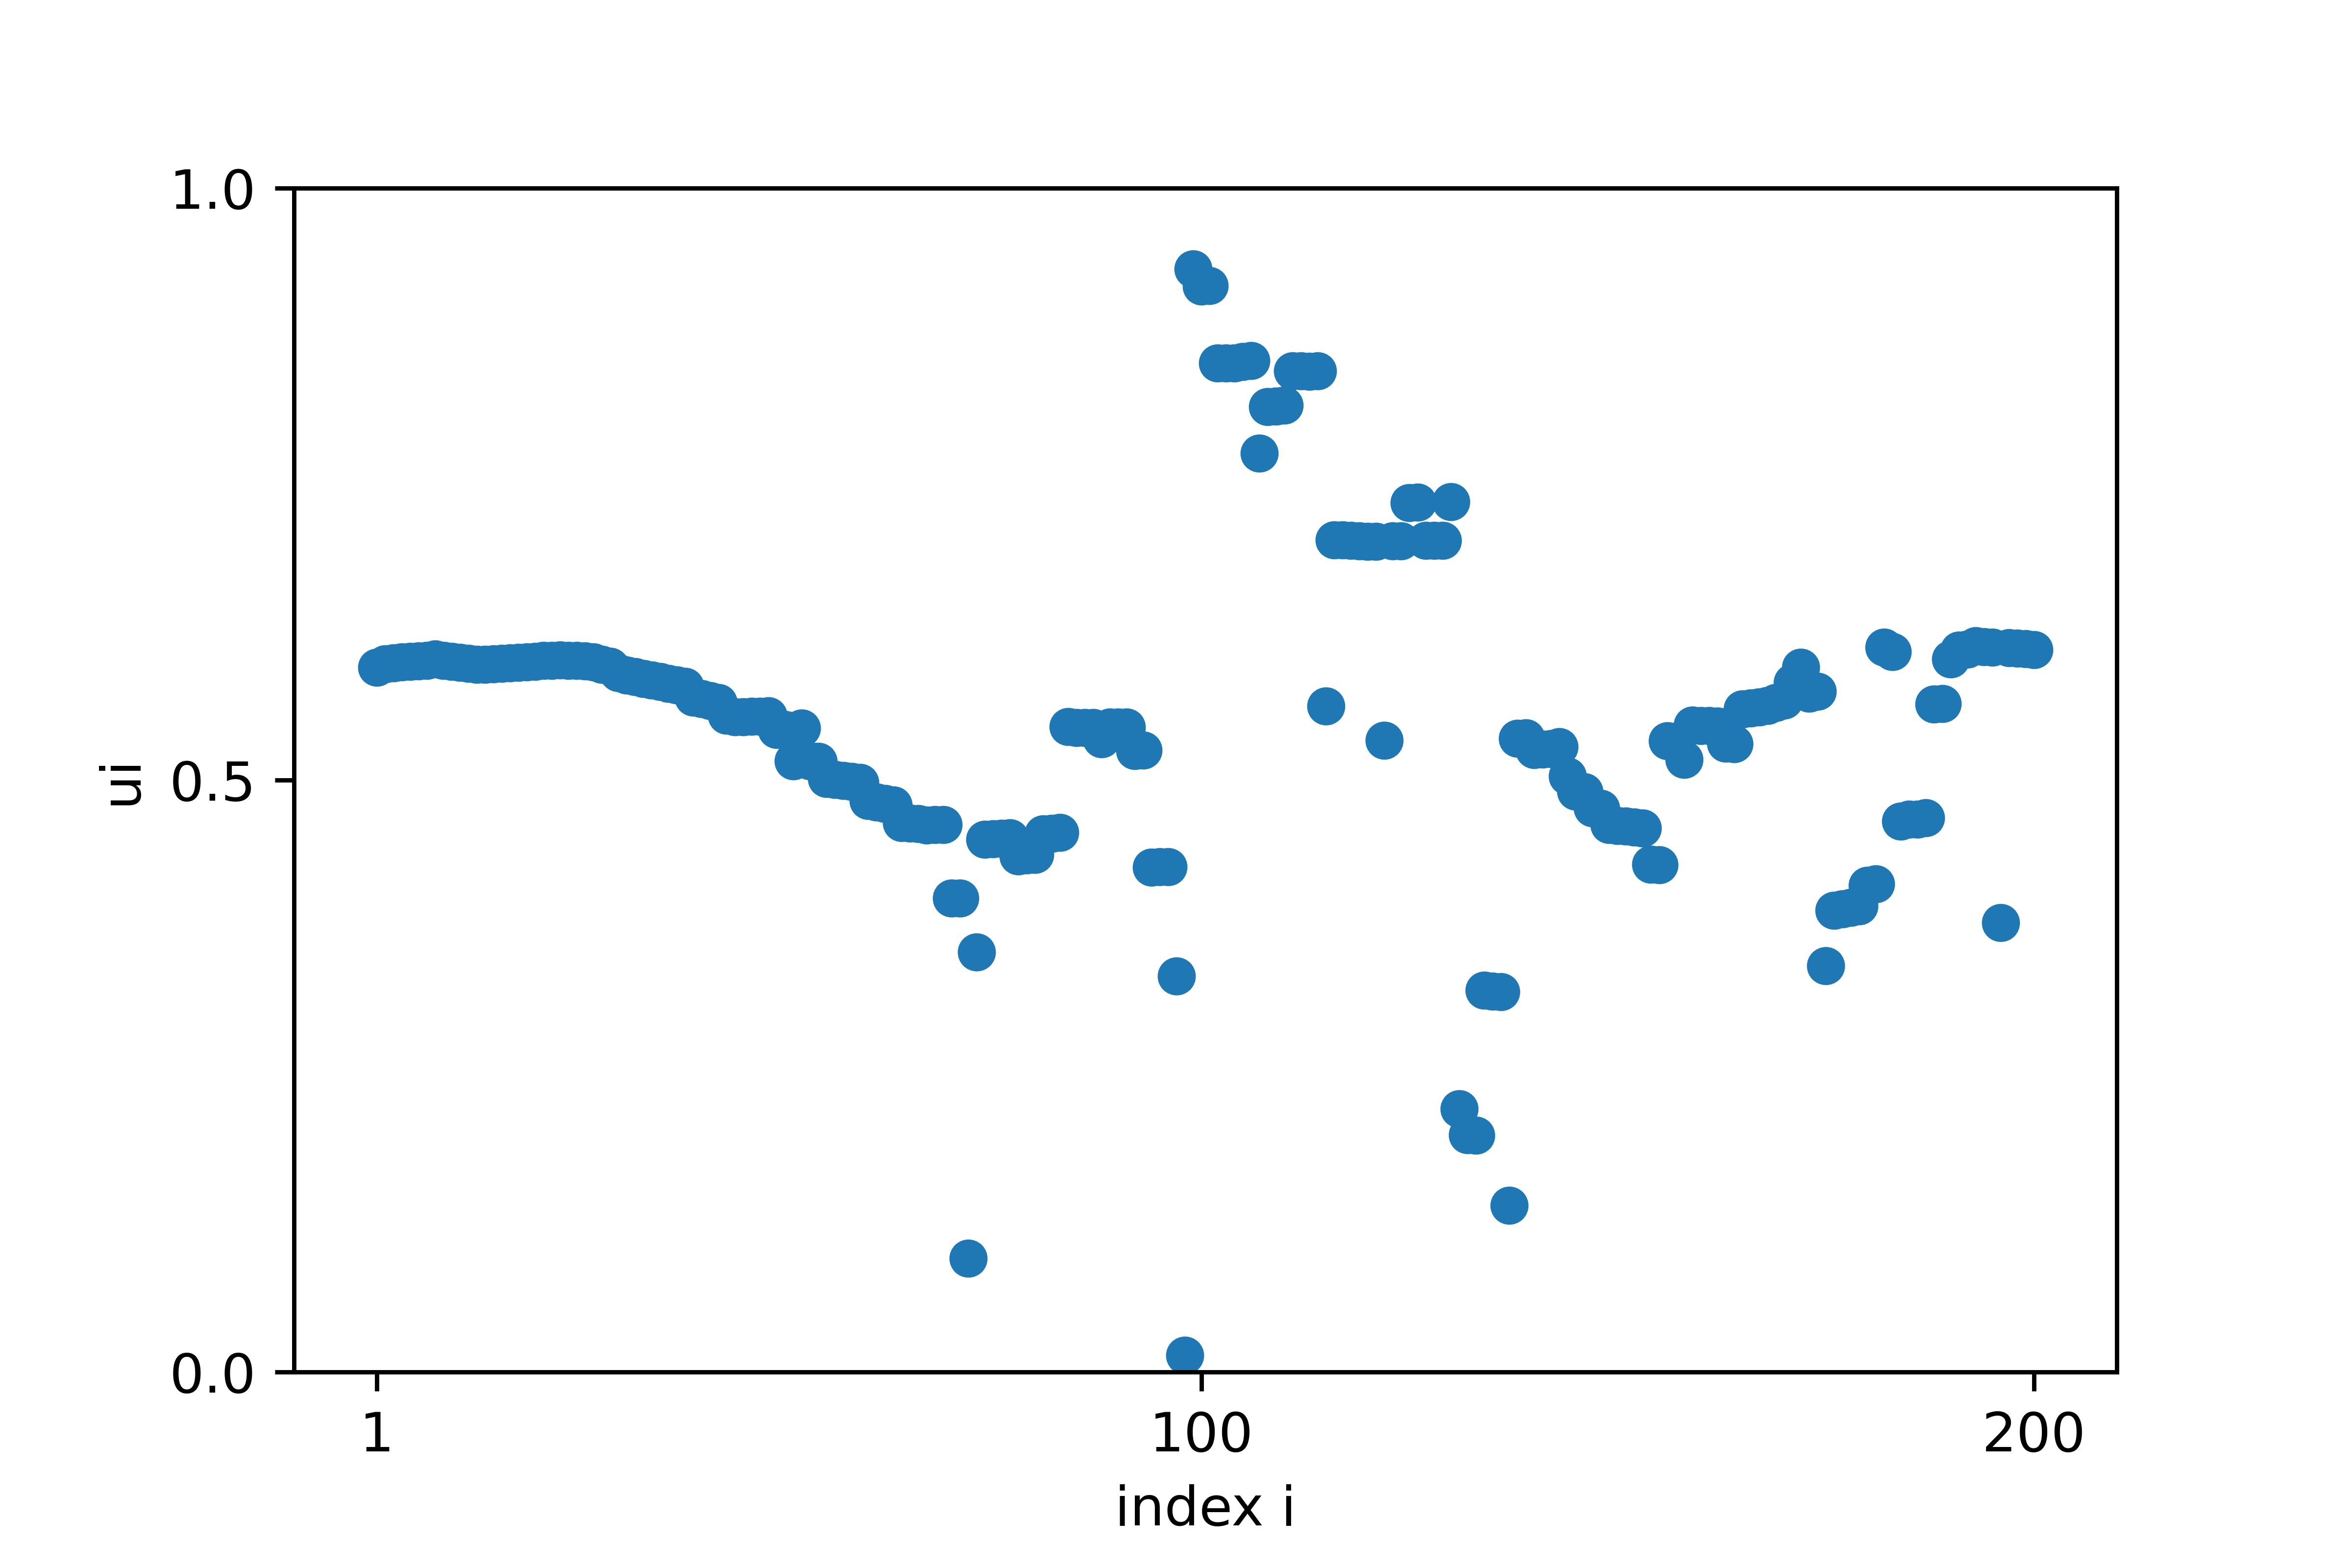
\includegraphics[width=\linewidth]{u_N=200_sigma=1.4_t=1000.png}
\caption{$t=1000$}
\end{subfigure}
\hfill
\begin{subfigure}{0.49 \textwidth}
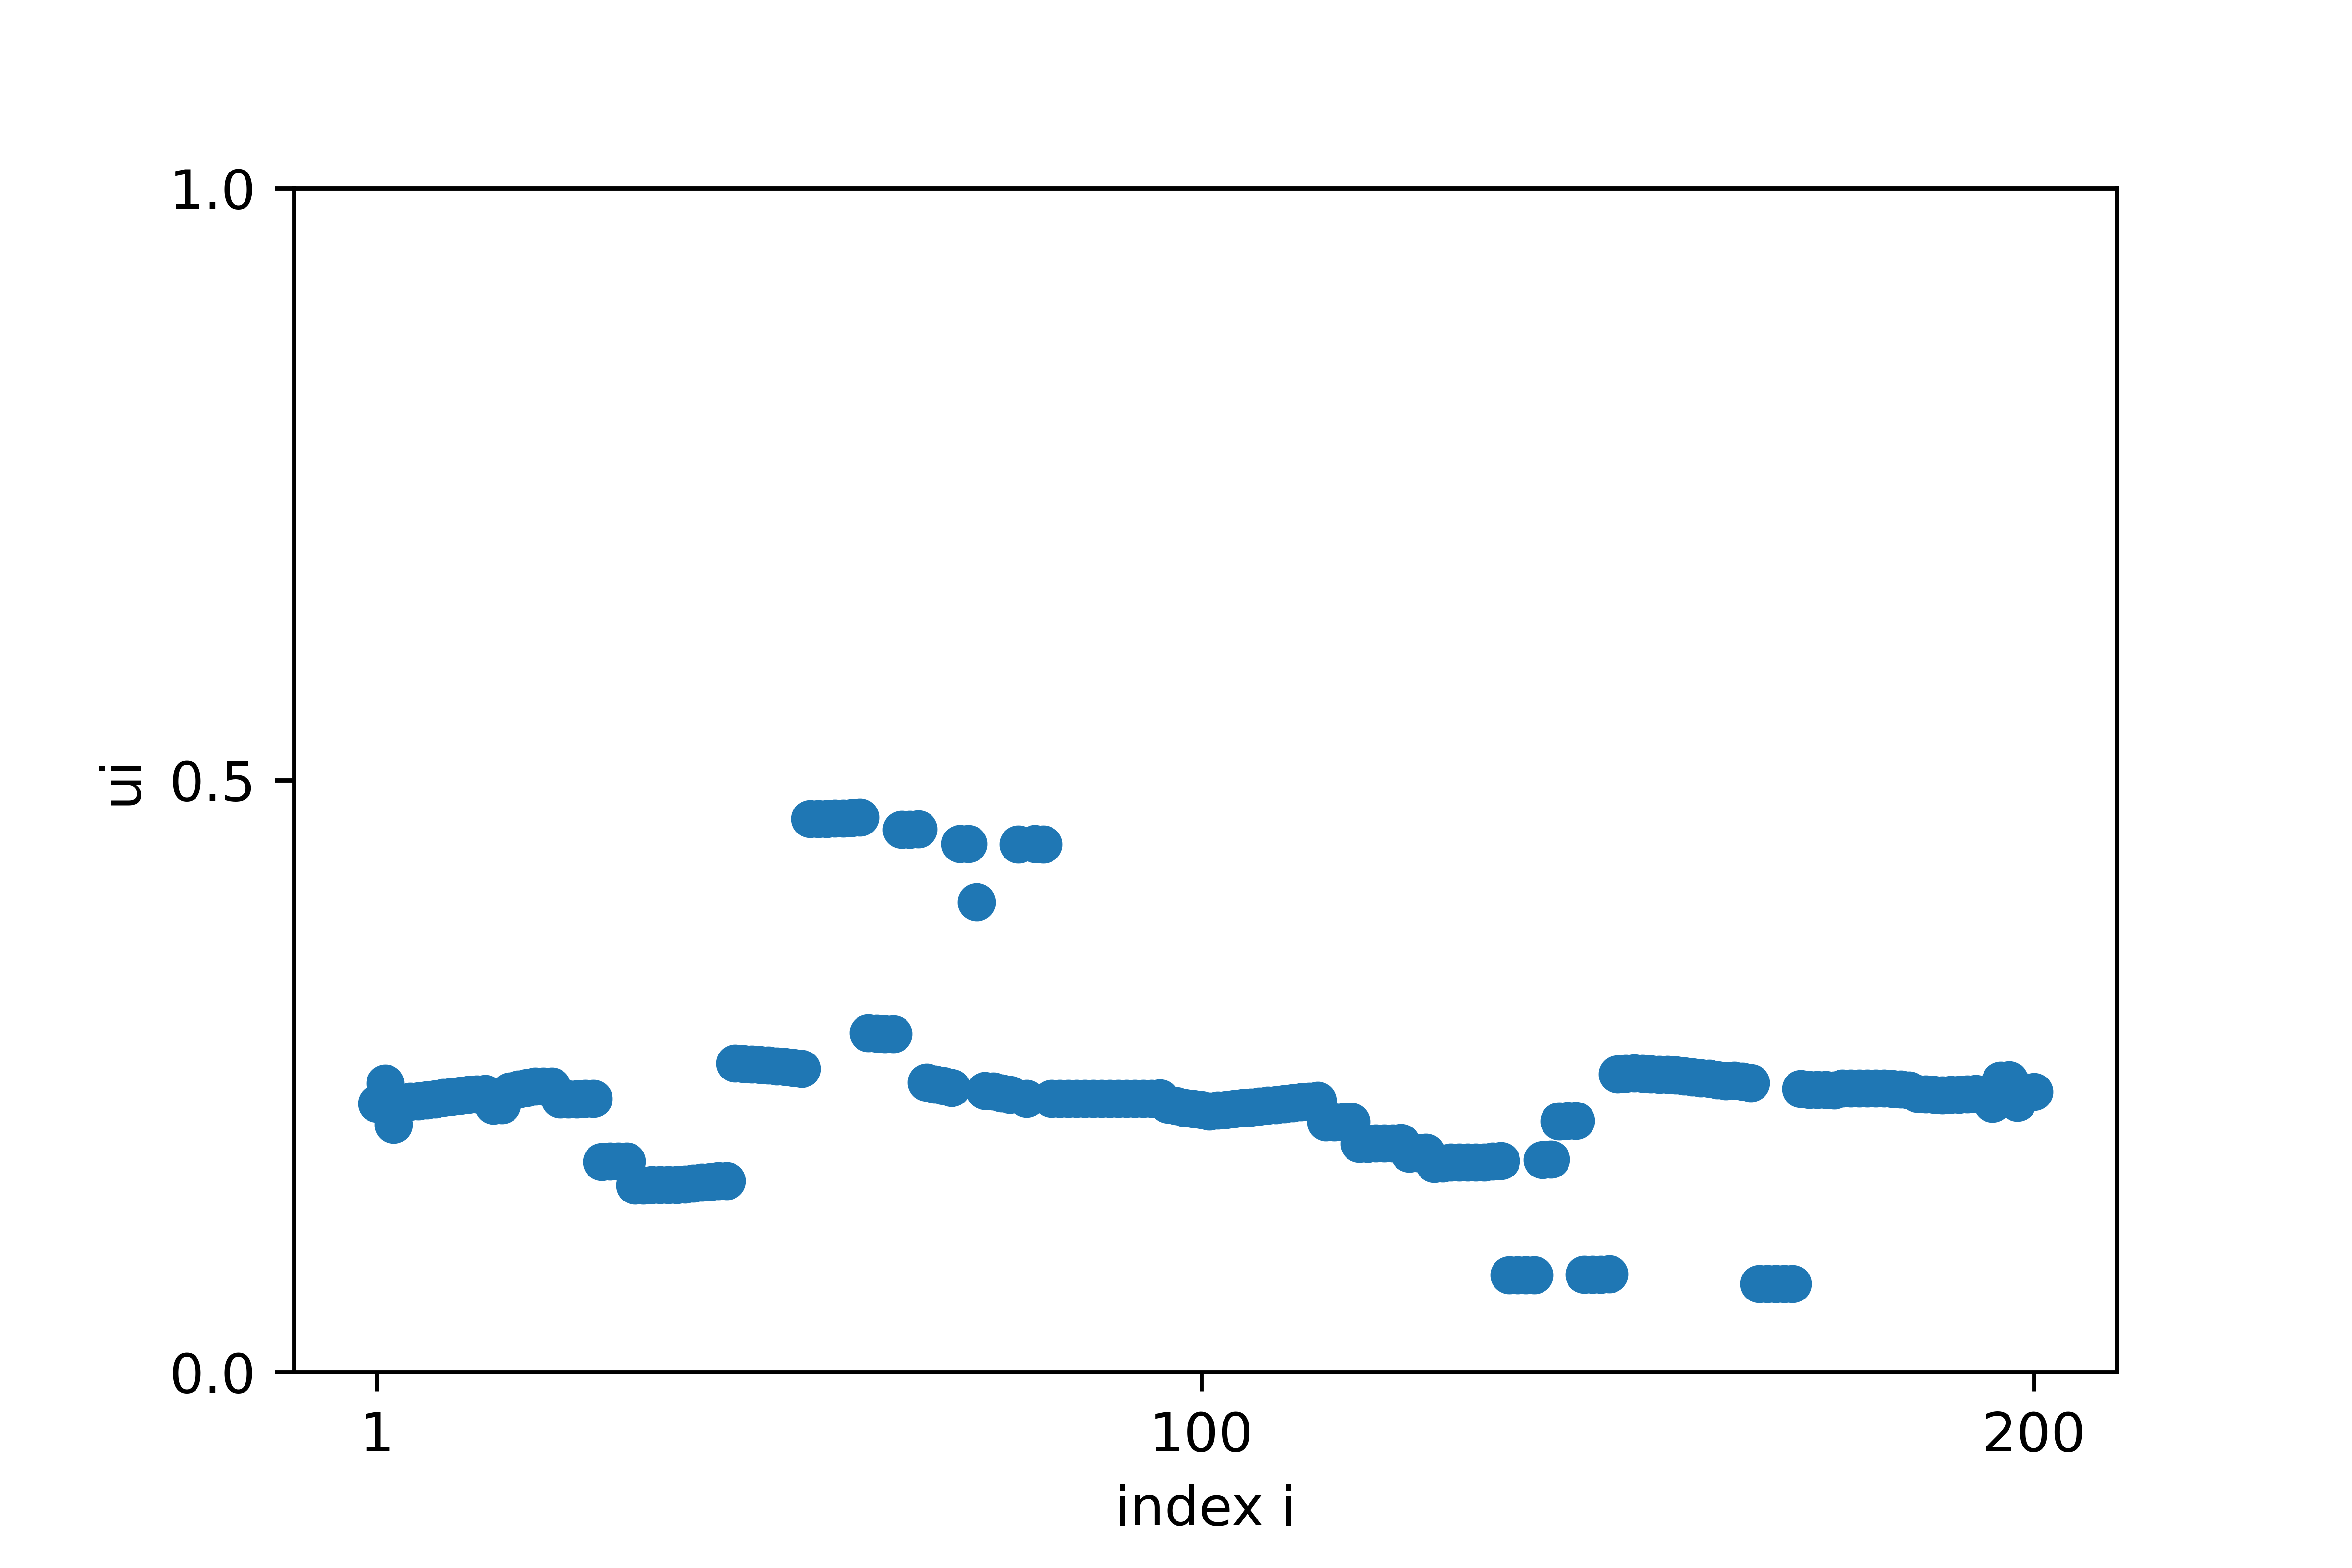
\includegraphics[width = \linewidth]{u_N=200_sigma=1.4_t=4000.png}
\caption{$t=4000$}
\end{subfigure}
\caption{Snapshots of the membrane potential $u_i$ at $t=1000$ and $t=4000$, for $N=200$, $\sigma=1.1$ and $r=0.35$.}
\label{1.4}
\end{figure}
\end{frame}

\begin{frame}{Chimera states in the $\lambda = 0$ model}
\begin{figure}[H]
\centering
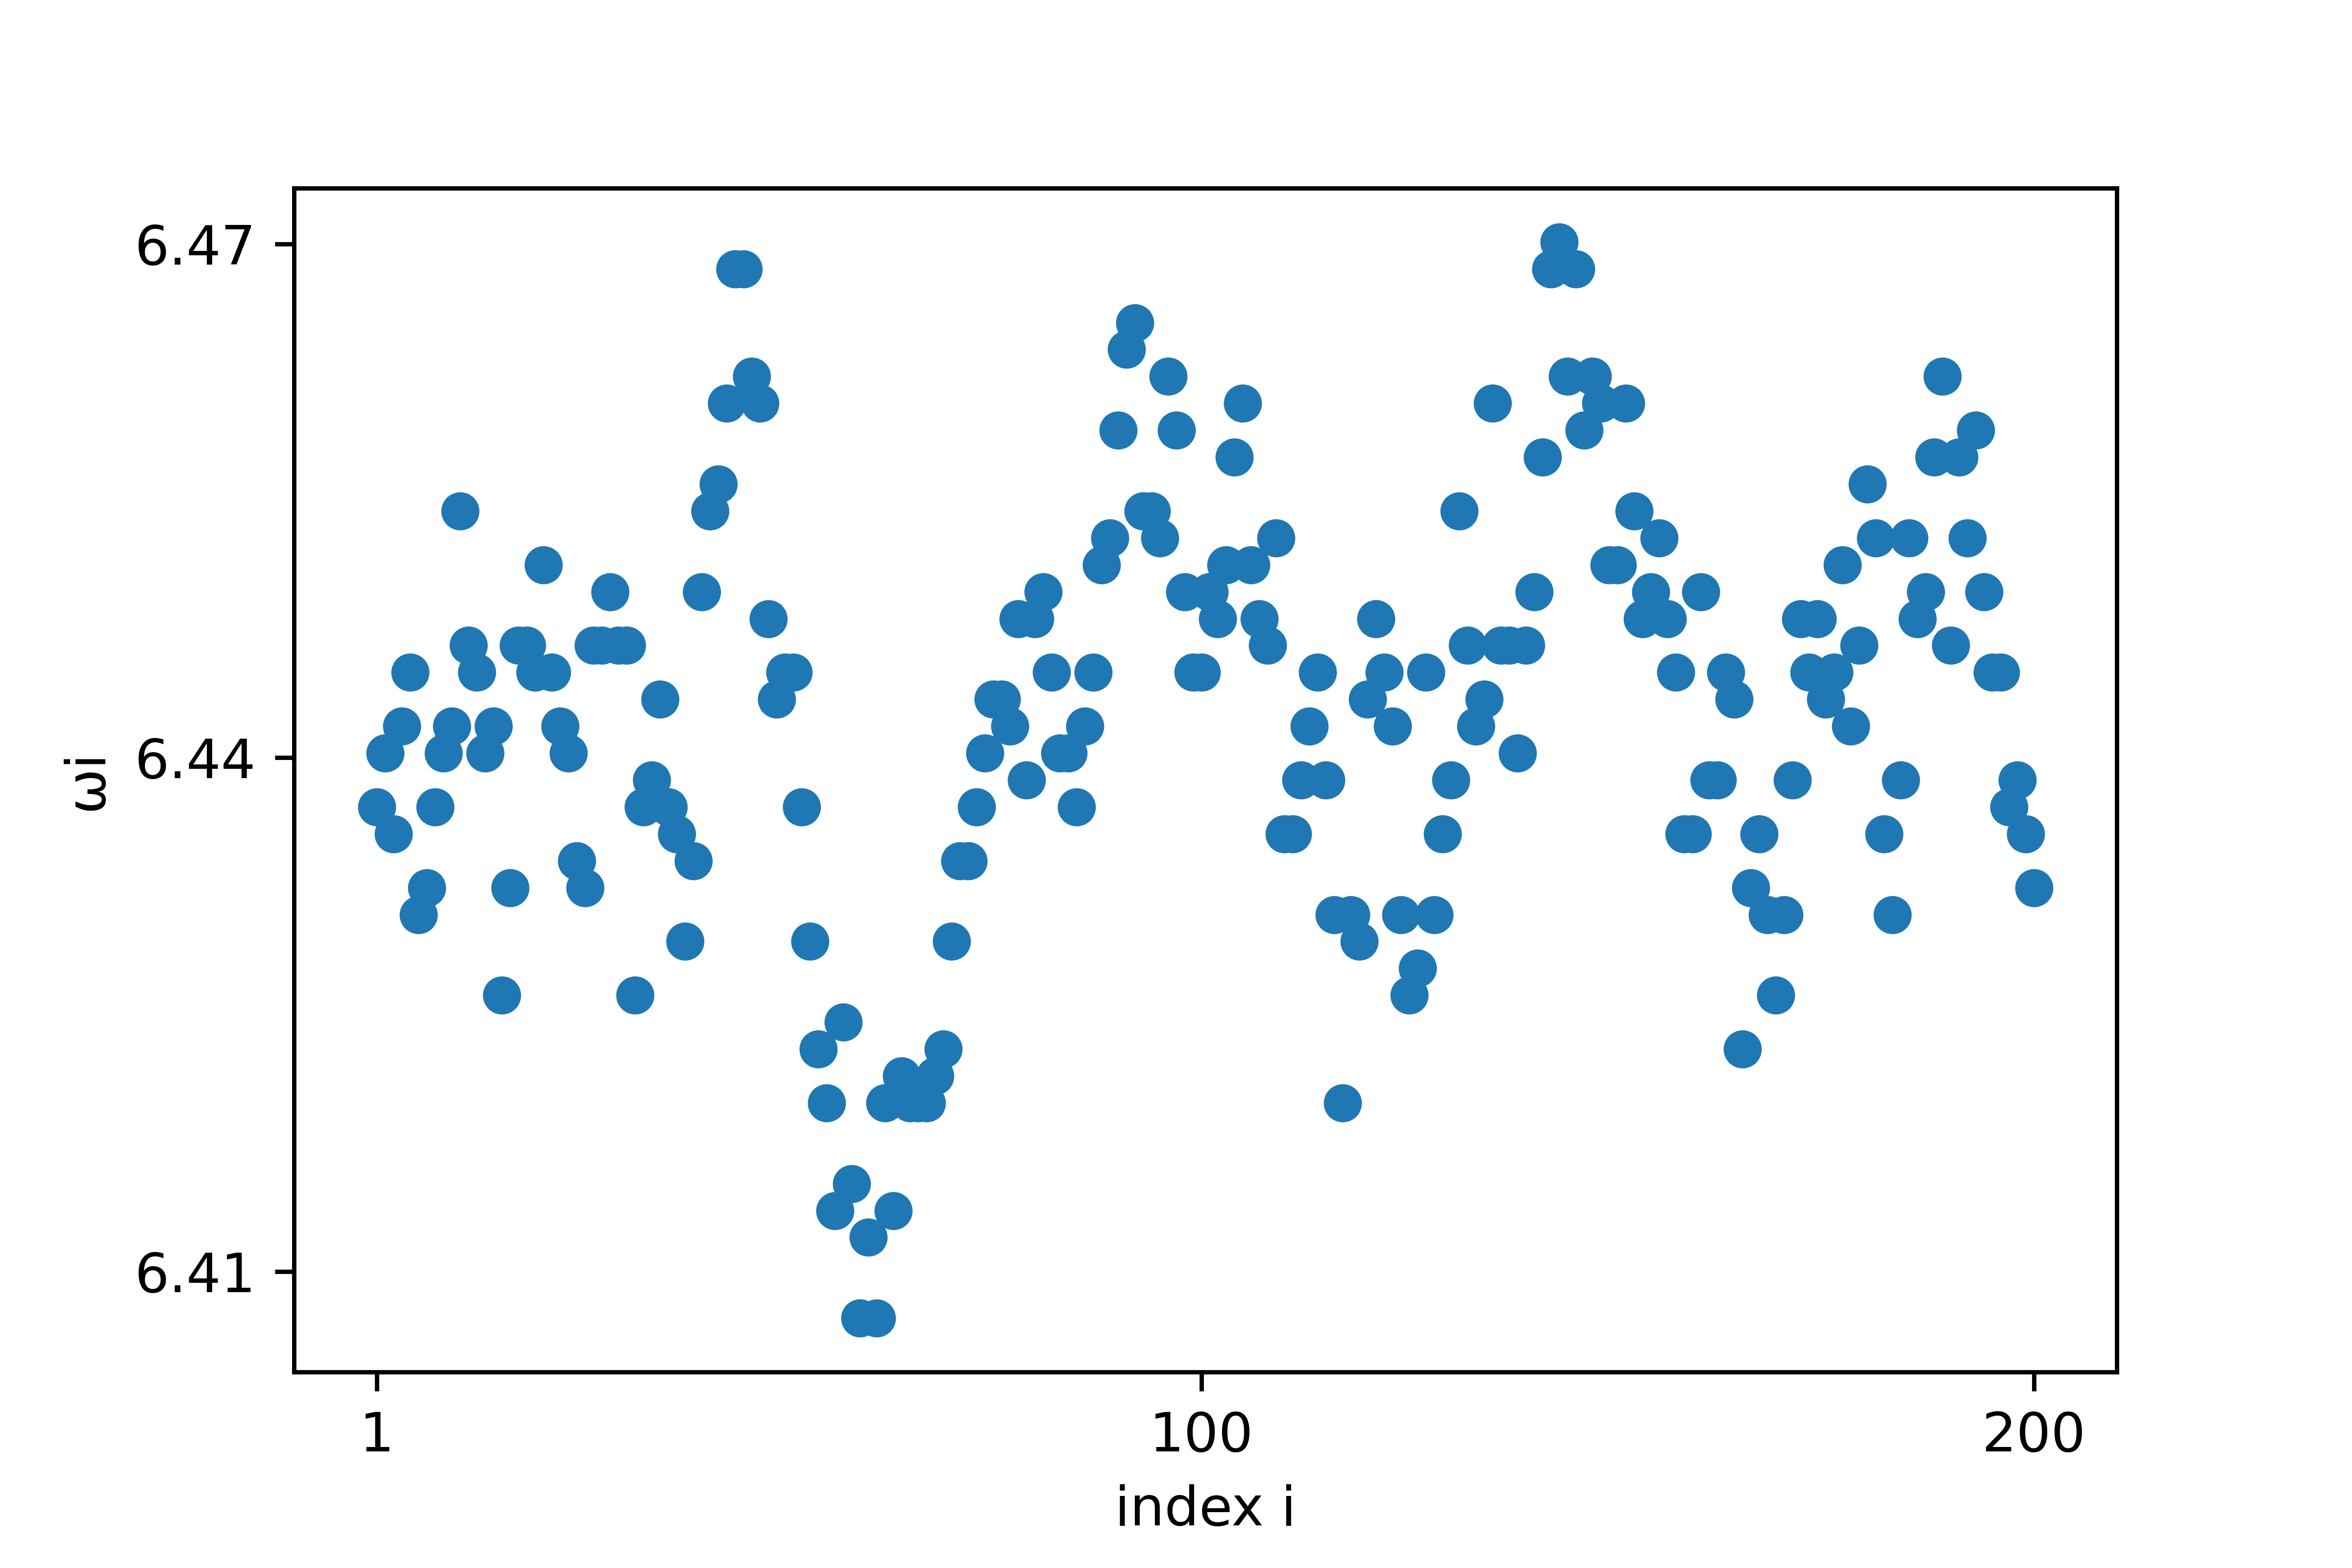
\includegraphics[width = 0.6 \textwidth]{w_N=200_sigma=1.4_t=4000.png}
\caption{Mean phase-velocity profile $\omega_i$ at $t=4000$, for $N=200$, $\sigma=1.1$ and $r=0.35$.}
\label{1.4omega}
\end{figure}
\end{frame}

\subsection{Varying $\lambda$}

\begin{frame}{Varying $\lambda$} \pause

\begin{figure}[H]
\centering
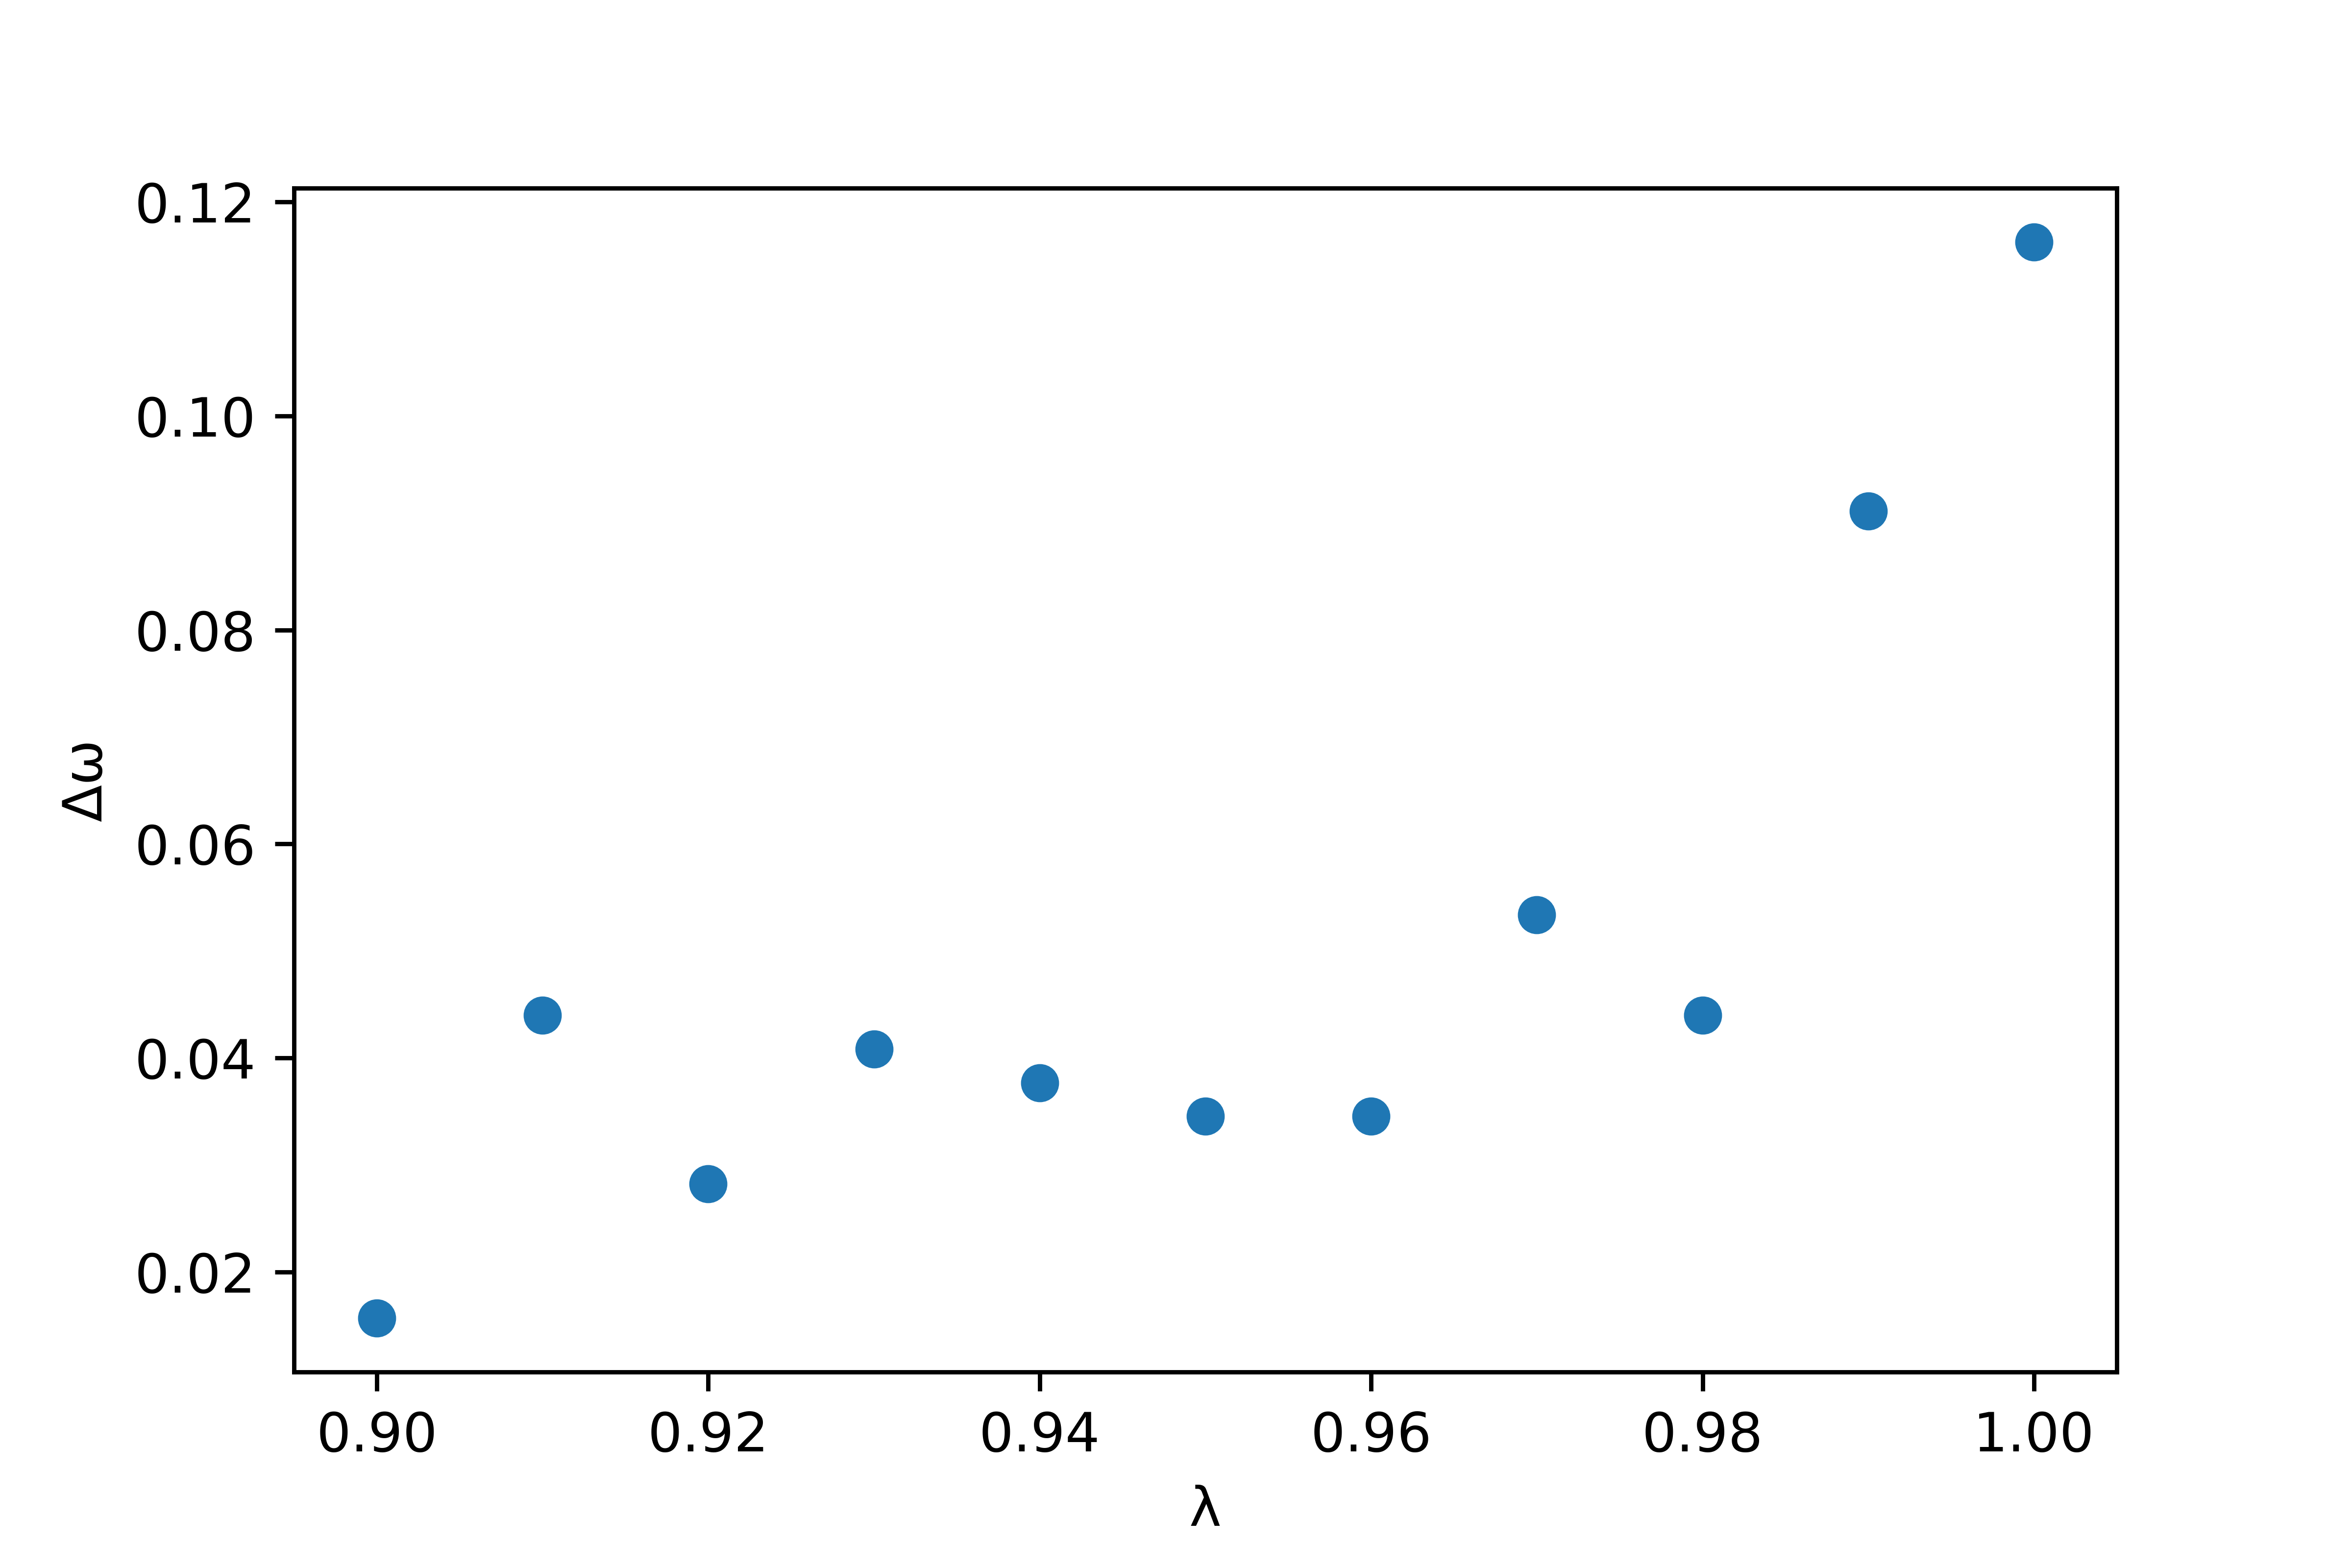
\includegraphics[width = 0.6 \textwidth]{deltawvslmd.png}
\caption{$\Delta \omega = \omega_{\text{max}}-\omega_{\text{min}}$ with varying $\lambda$.}
\label{vslmd}
\end{figure}

\end{frame}

\begin{frame}{Varying $\lambda$}

\begin{figure}[H]
\begin{subfigure}{.32\textwidth}
  \centering
  % include first image
  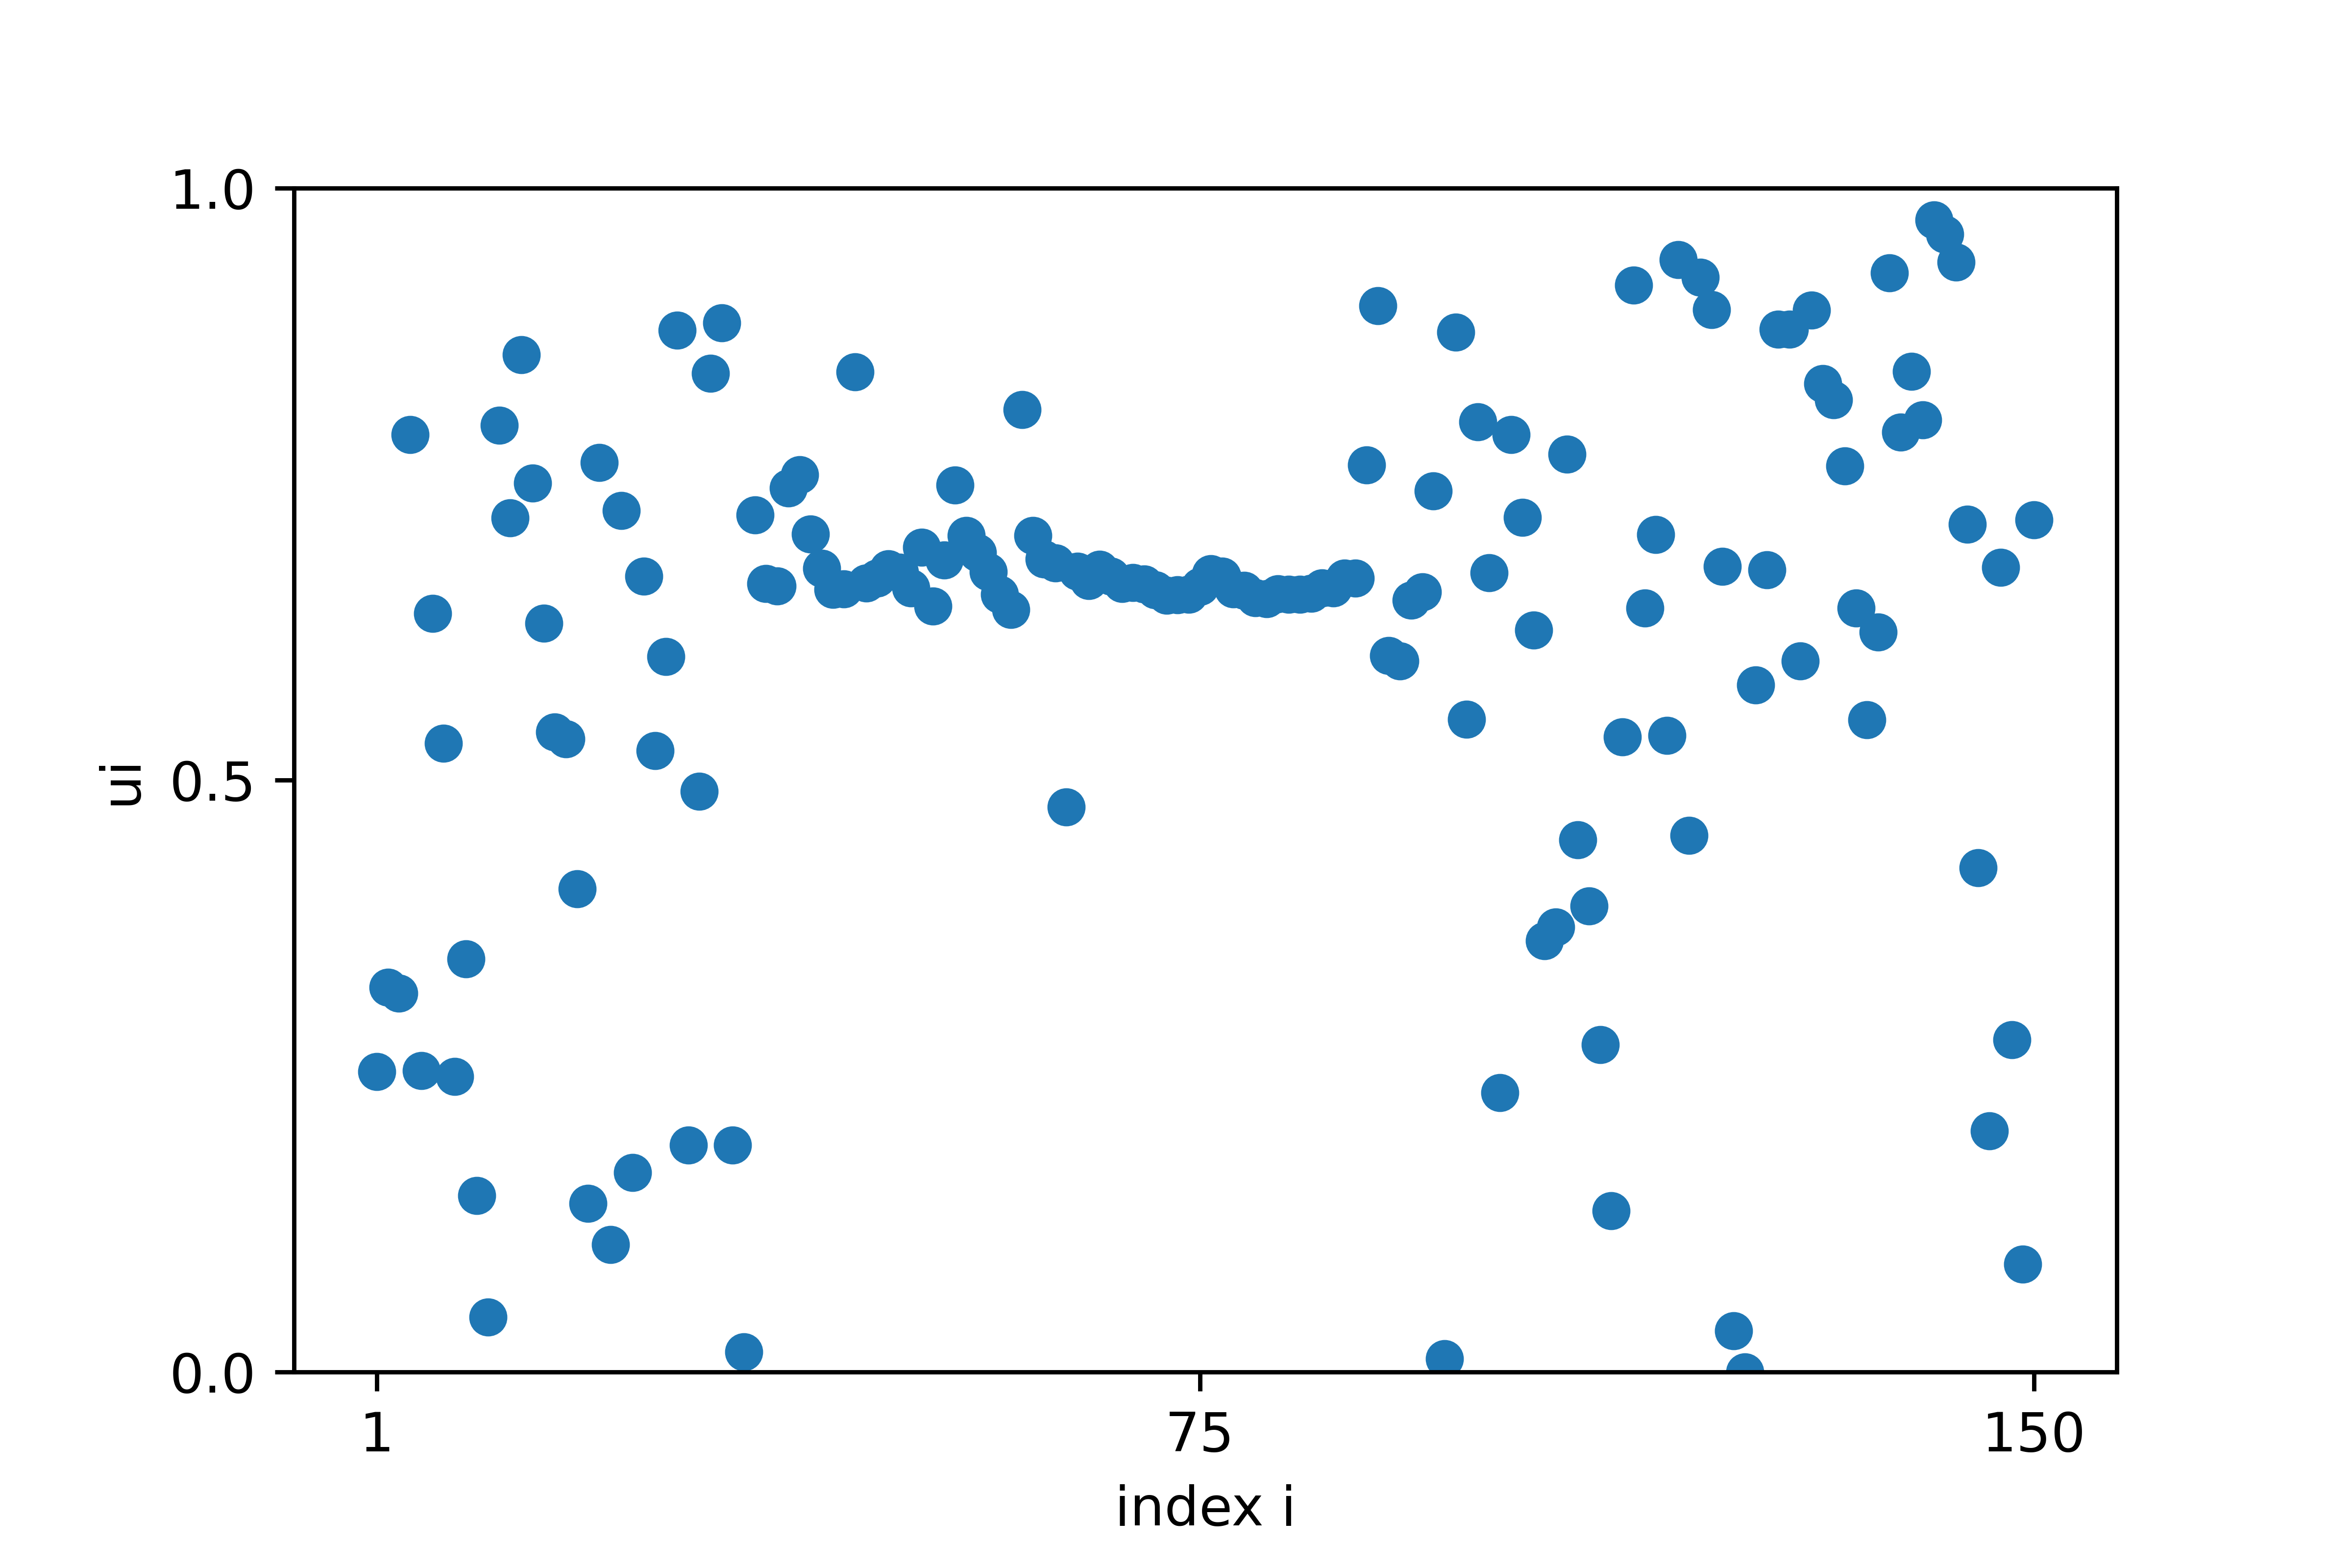
\includegraphics[width=1\linewidth]{u_lambda=1.0_t=2000.png}  
  \caption{$\lambda=1.00$}
\end{subfigure}
\hfill
\begin{subfigure}{.32\textwidth}
  \centering
  % include second image
  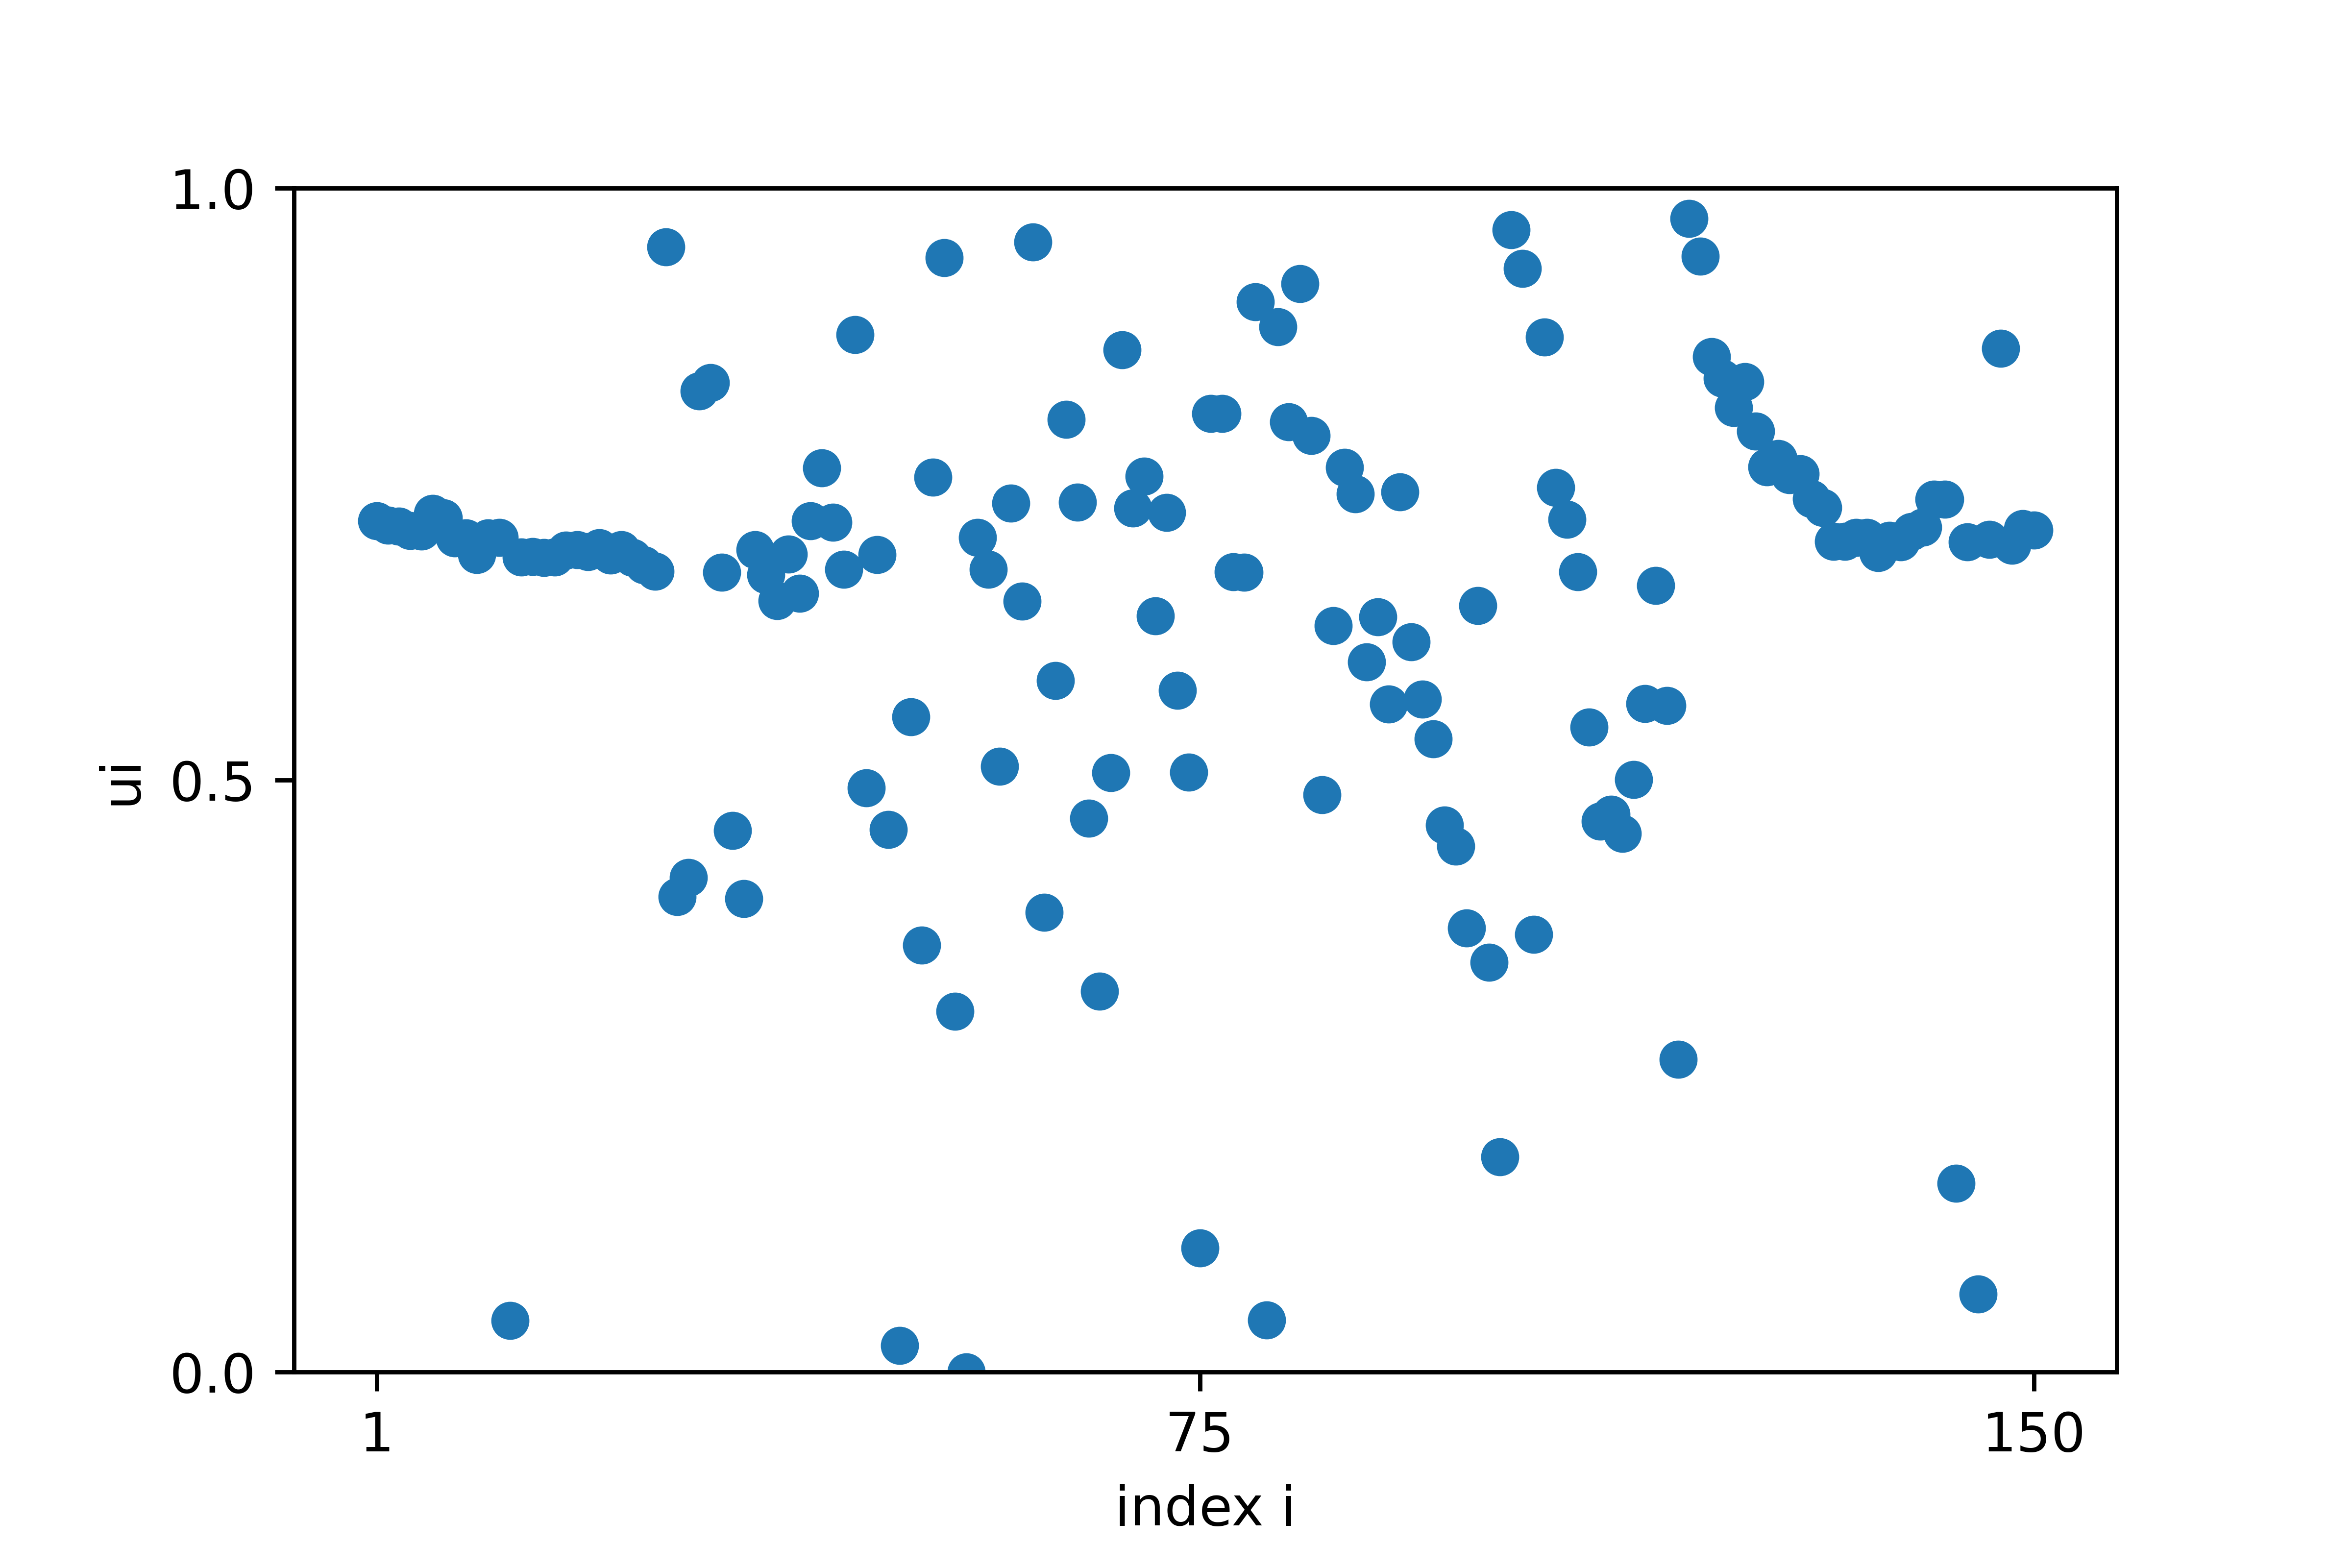
\includegraphics[width=1\linewidth]{u_lambda=0.99_t=2000.png}  
  \caption{$\lambda=0.99$}
\end{subfigure}
\hfill
\begin{subfigure}{.32\textwidth}
  \centering
  % include first image
  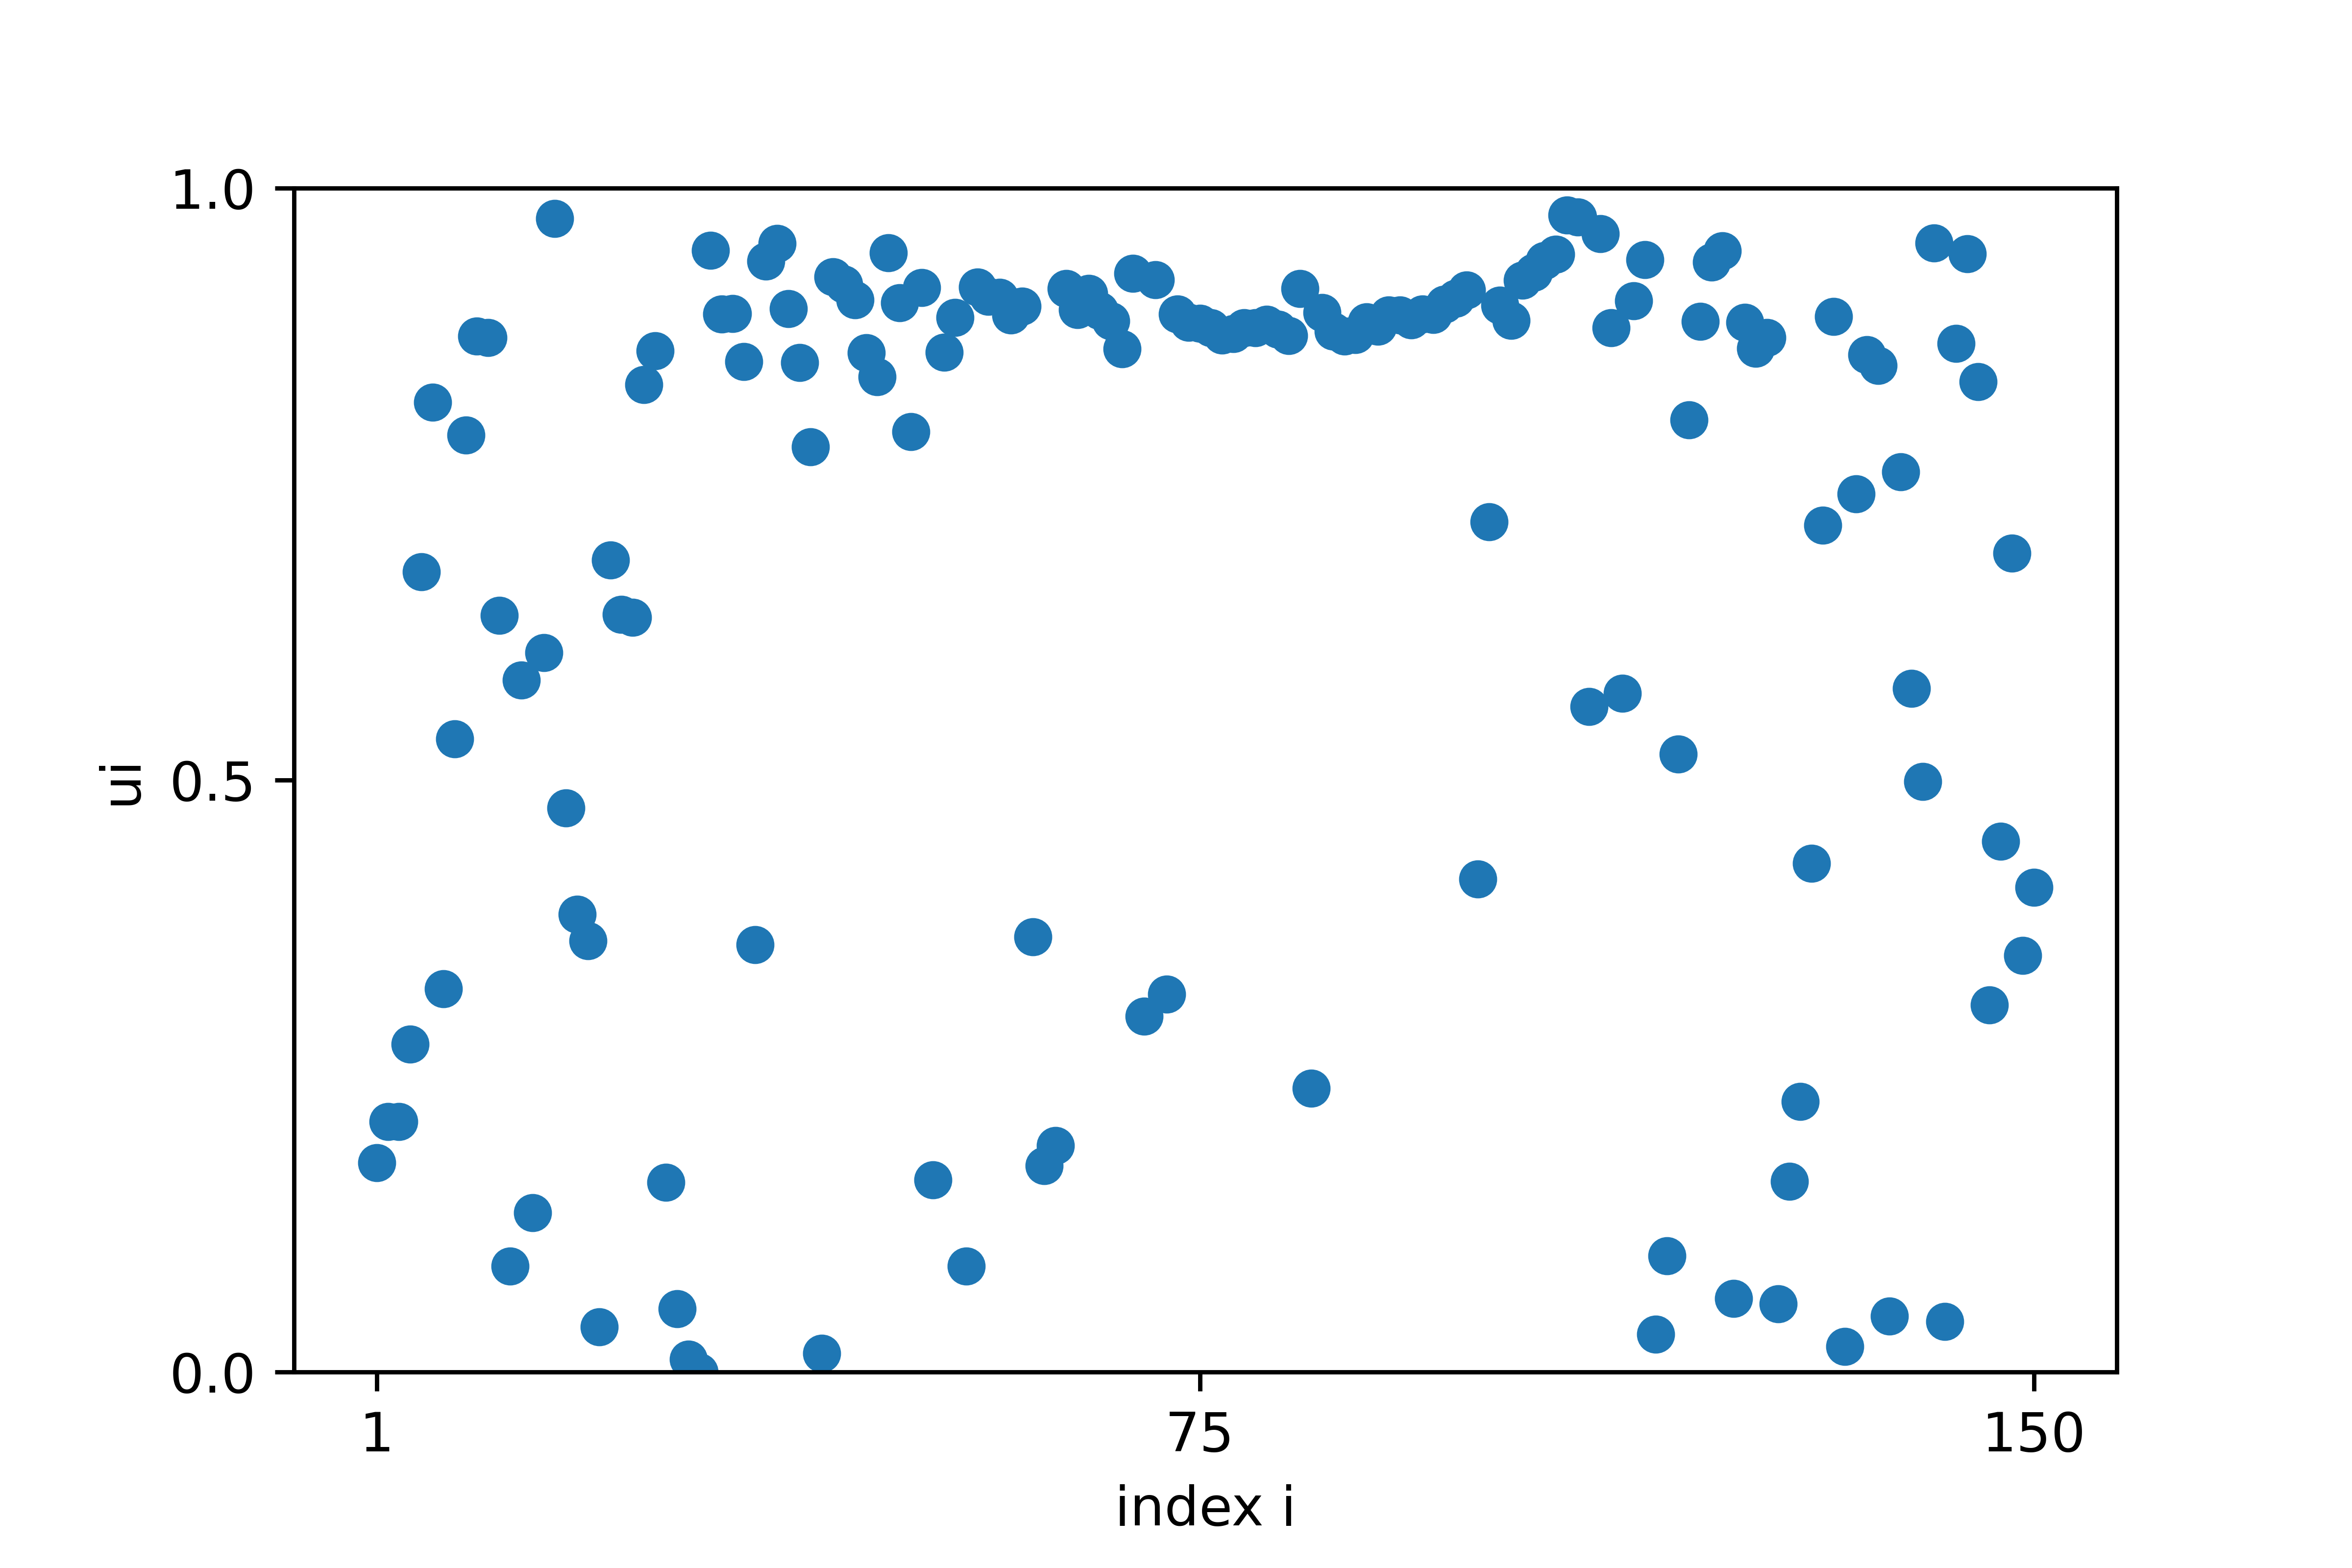
\includegraphics[width=1\linewidth]{u_lambda=0.98_t=2000}  
  \caption{$\lambda=0.98$}
\end{subfigure}
\begin{subfigure}{.32\textwidth}
  \centering
  % include first image
  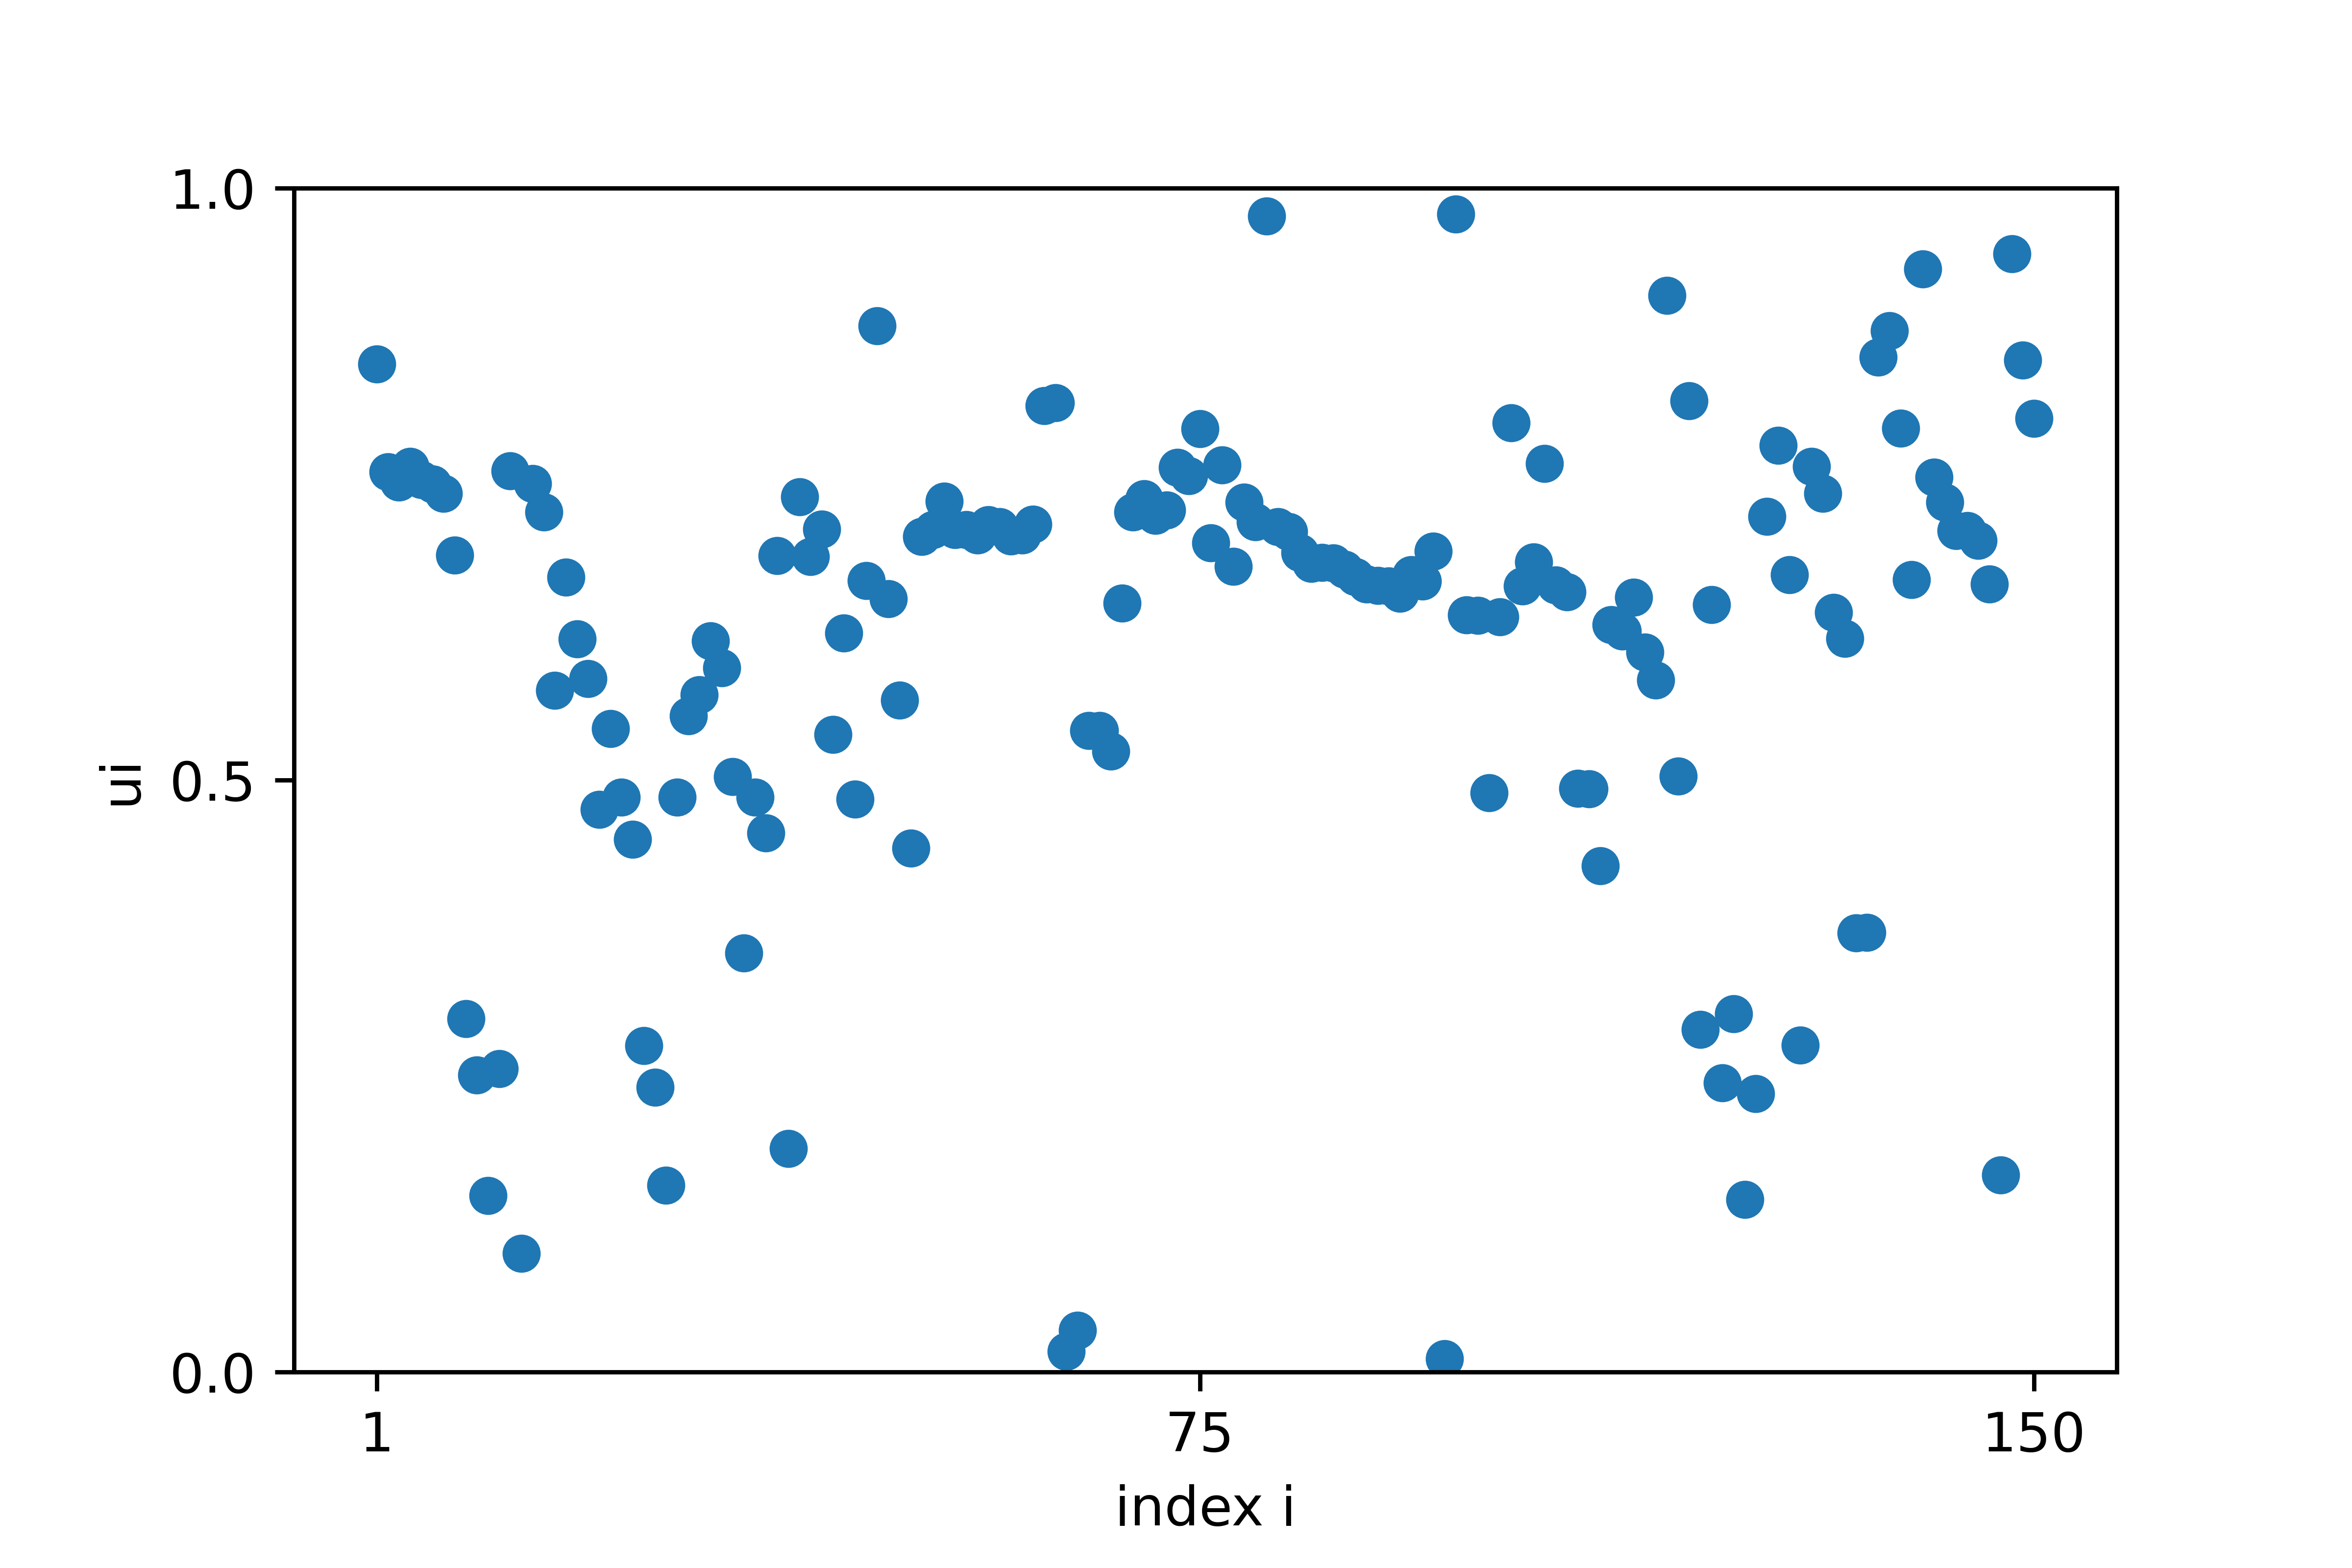
\includegraphics[width=1\linewidth]{u_lambda=0.97_t=2000.png}  
  \caption{$\lambda=0.97$}
\end{subfigure}
\hfill
\begin{subfigure}{.32\textwidth}
  \centering
  % include first image
  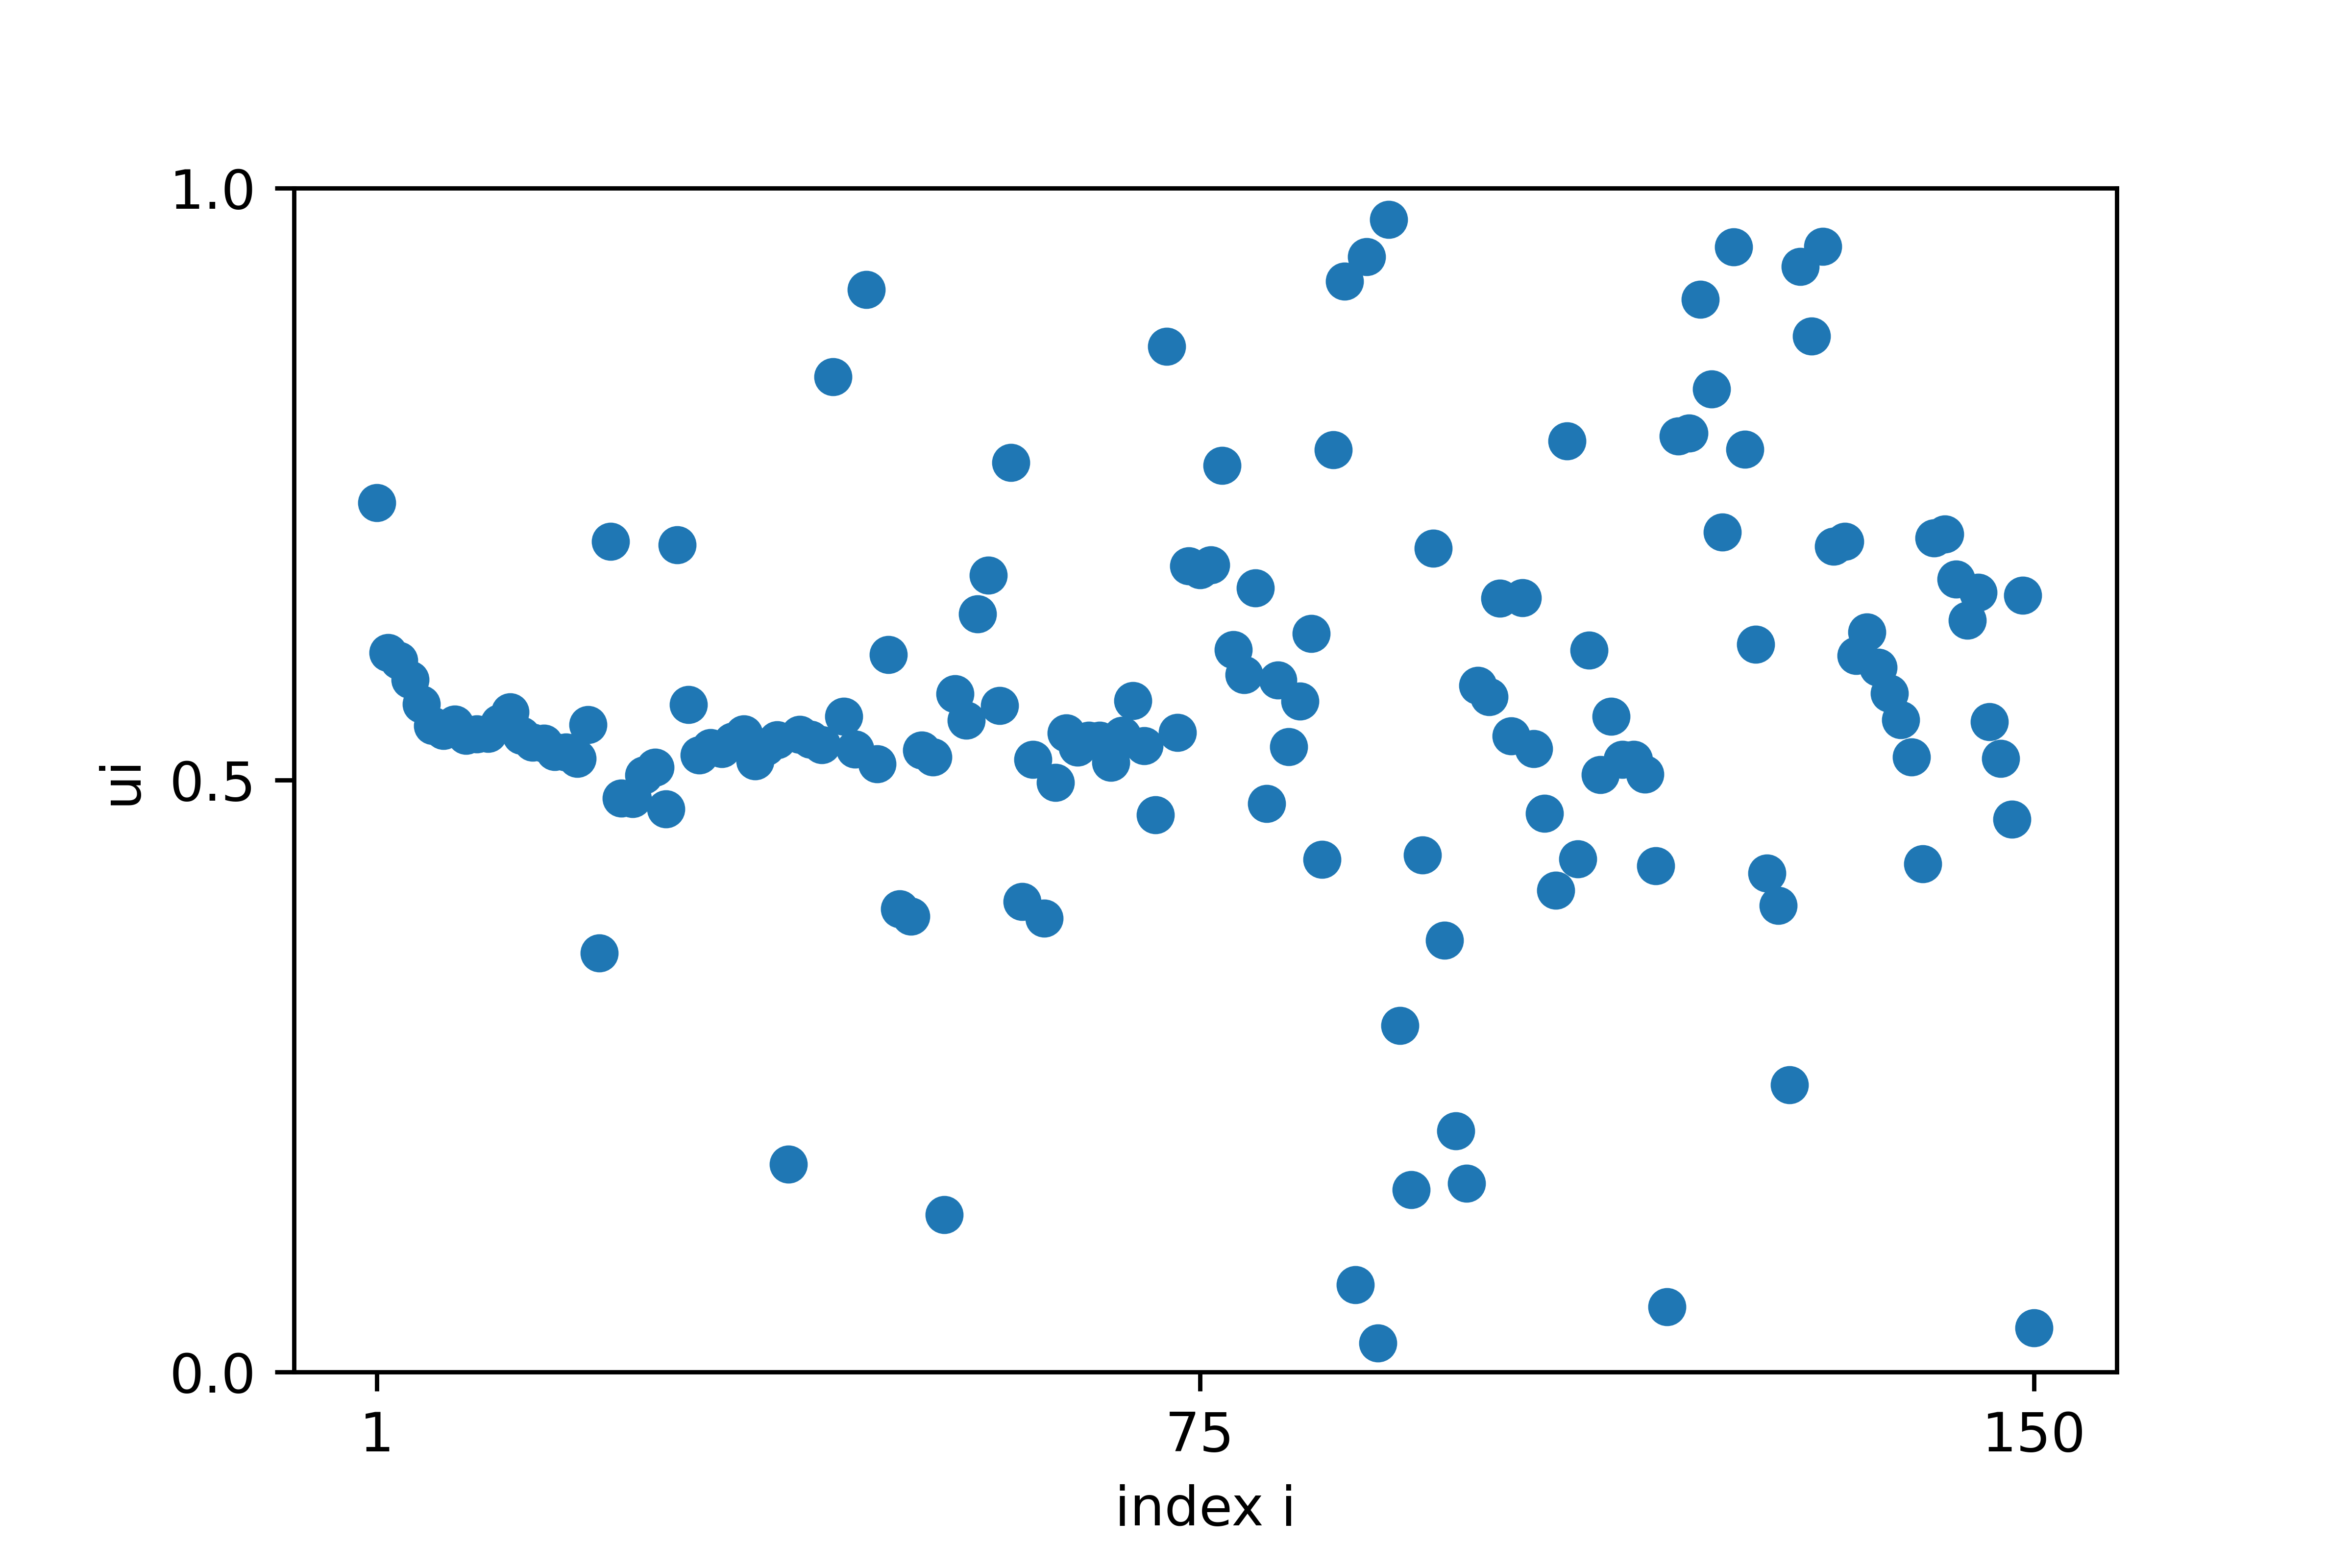
\includegraphics[width=1\linewidth]{u_lambda=0.96_t=2000.png}  
  \caption{$\lambda=0.96$}
\end{subfigure}
\hfill
\begin{subfigure}{.32\textwidth}
  \centering
  % include first image
  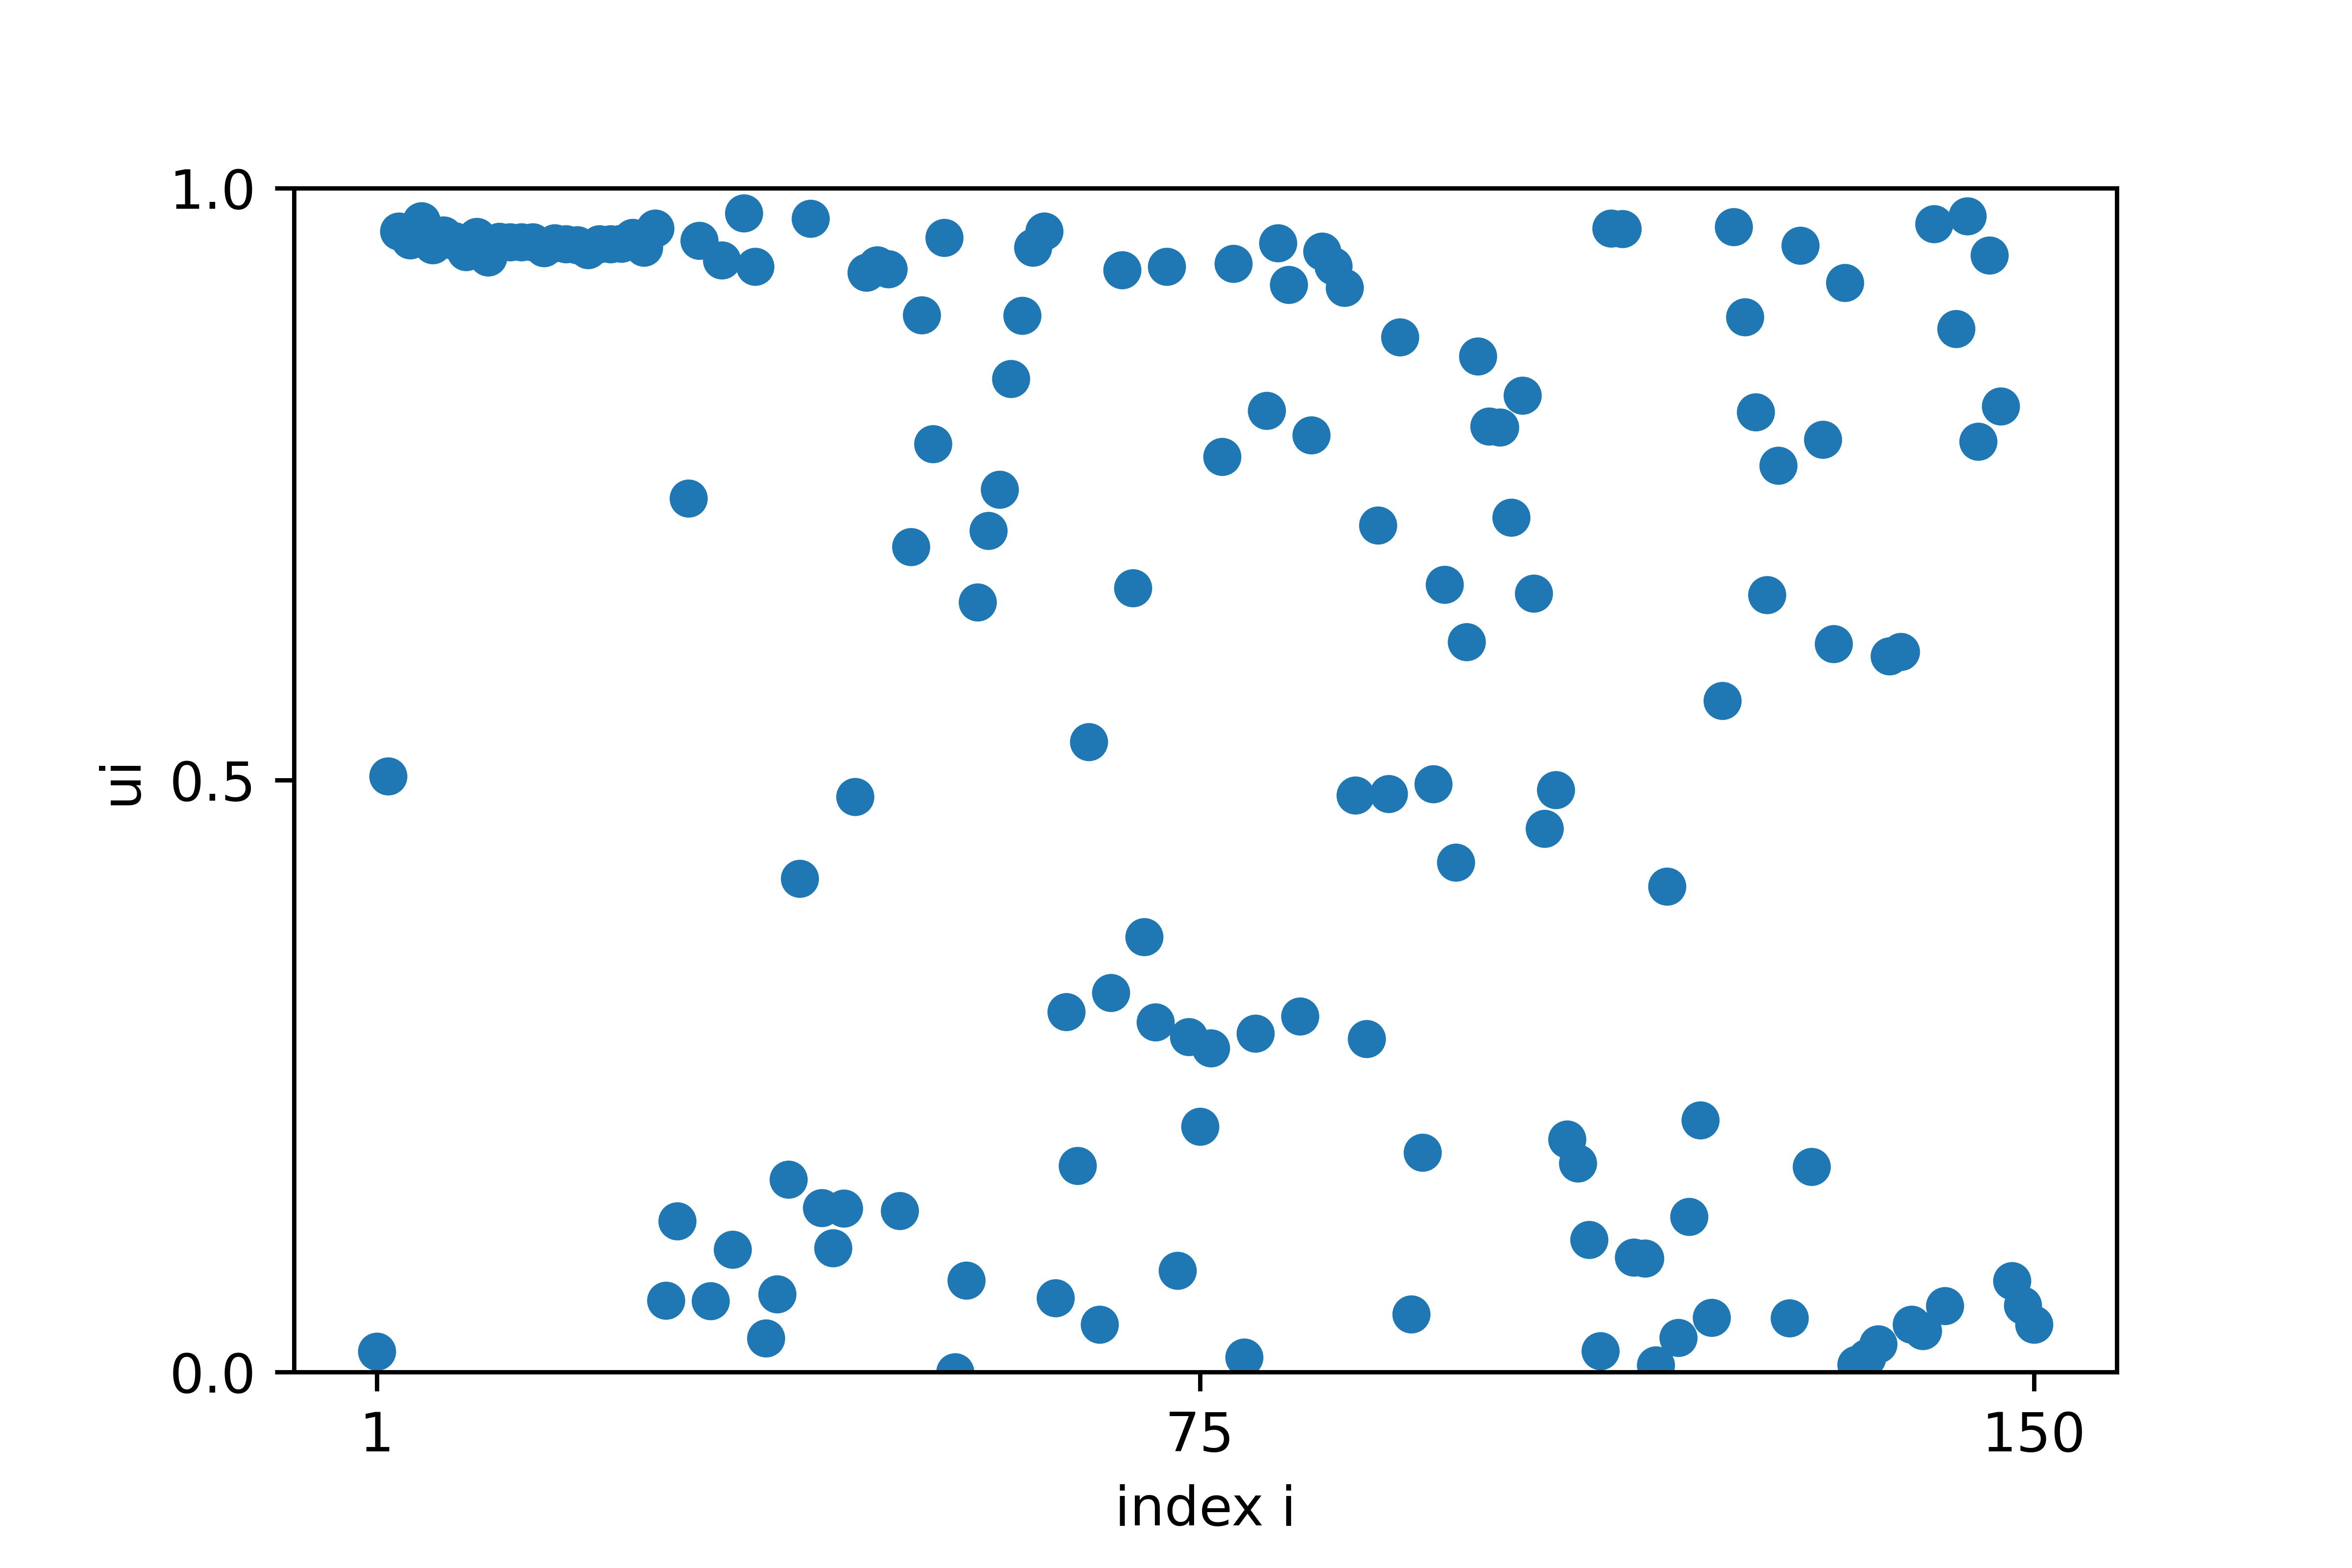
\includegraphics[width=1\linewidth]{u_lambda=0.95_t=2000.png}  
  \caption{$\lambda=0.95$}
\end{subfigure}

\caption{Snapshots of the membrane potential $u_i$ at $t=2000$ time units, for $N=150$, $r=0.4$ and $\sigma = 0.7$ and for various values of $\lambda$.}
\label{uivslmd}
\end{figure}

\end{frame}

\begin{frame}{Varying $\lambda$}
\begin{figure}[H]
\begin{subfigure}{.32\textwidth}
  \centering
  % include first image
  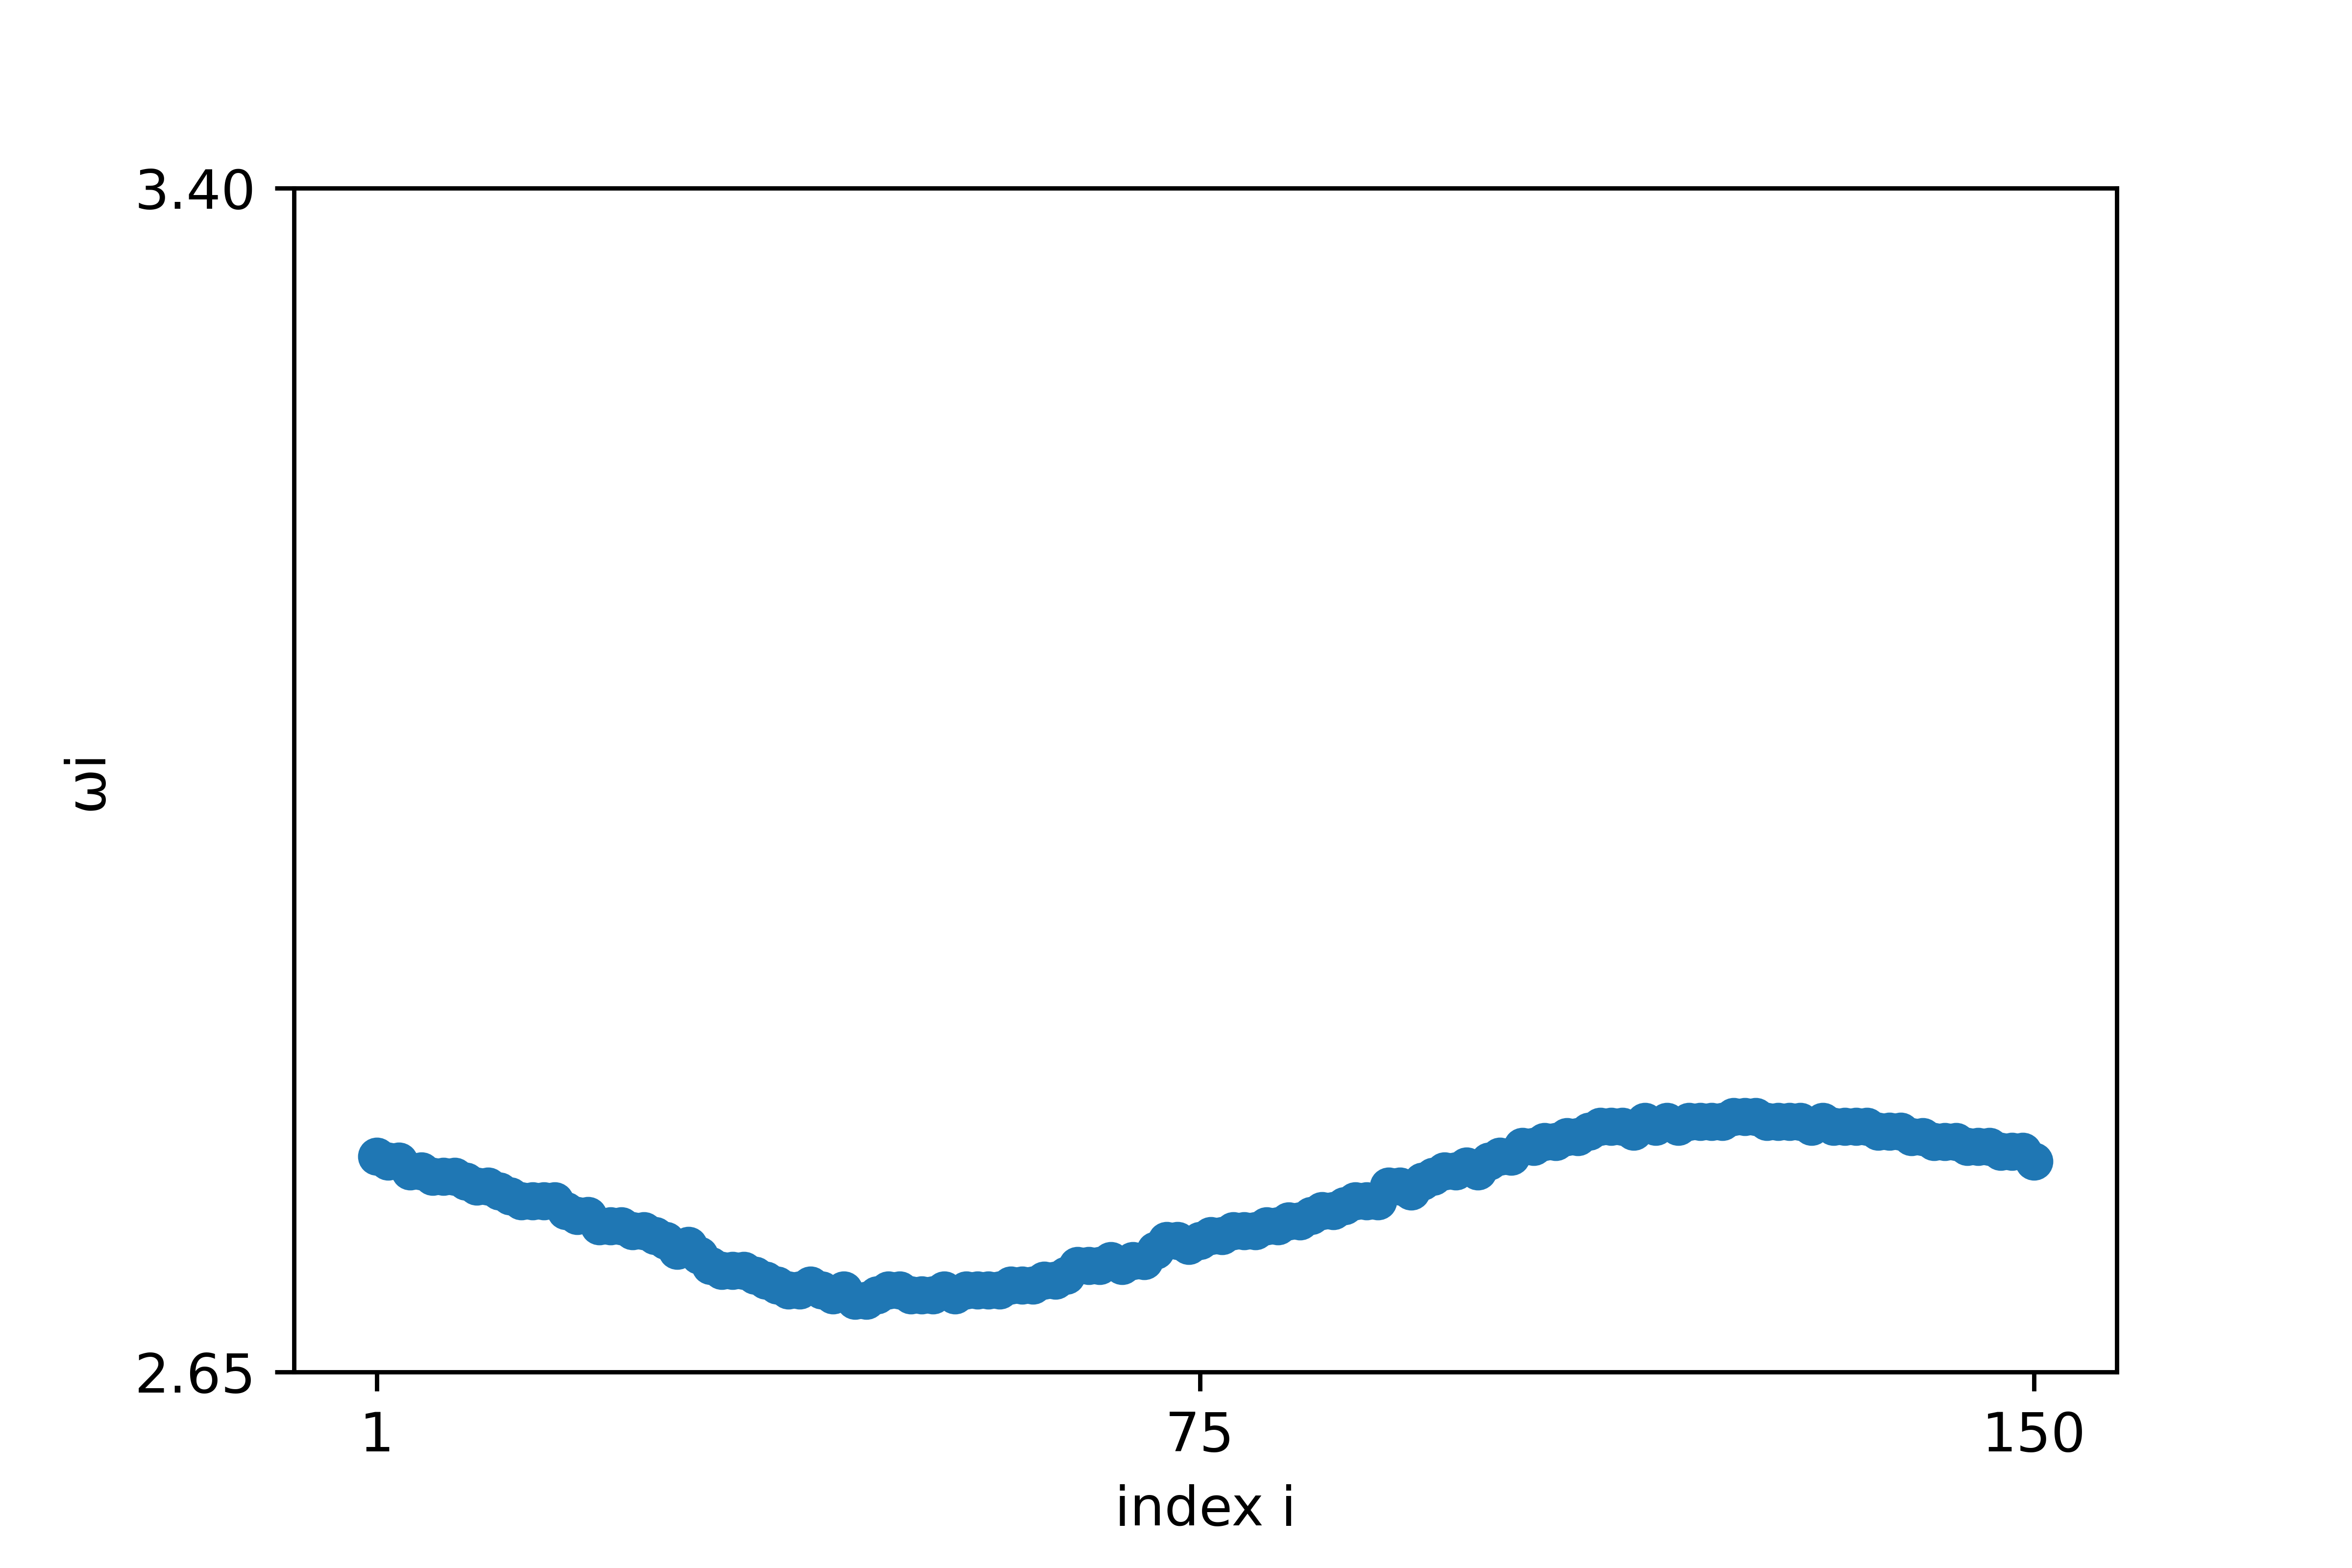
\includegraphics[width=1\linewidth]{w_lambda=1.0_t=2000.png}  
  \caption{$\lambda=1.00$}
\end{subfigure}
\hfill
\begin{subfigure}{.32\textwidth}
  \centering
  % include second image
  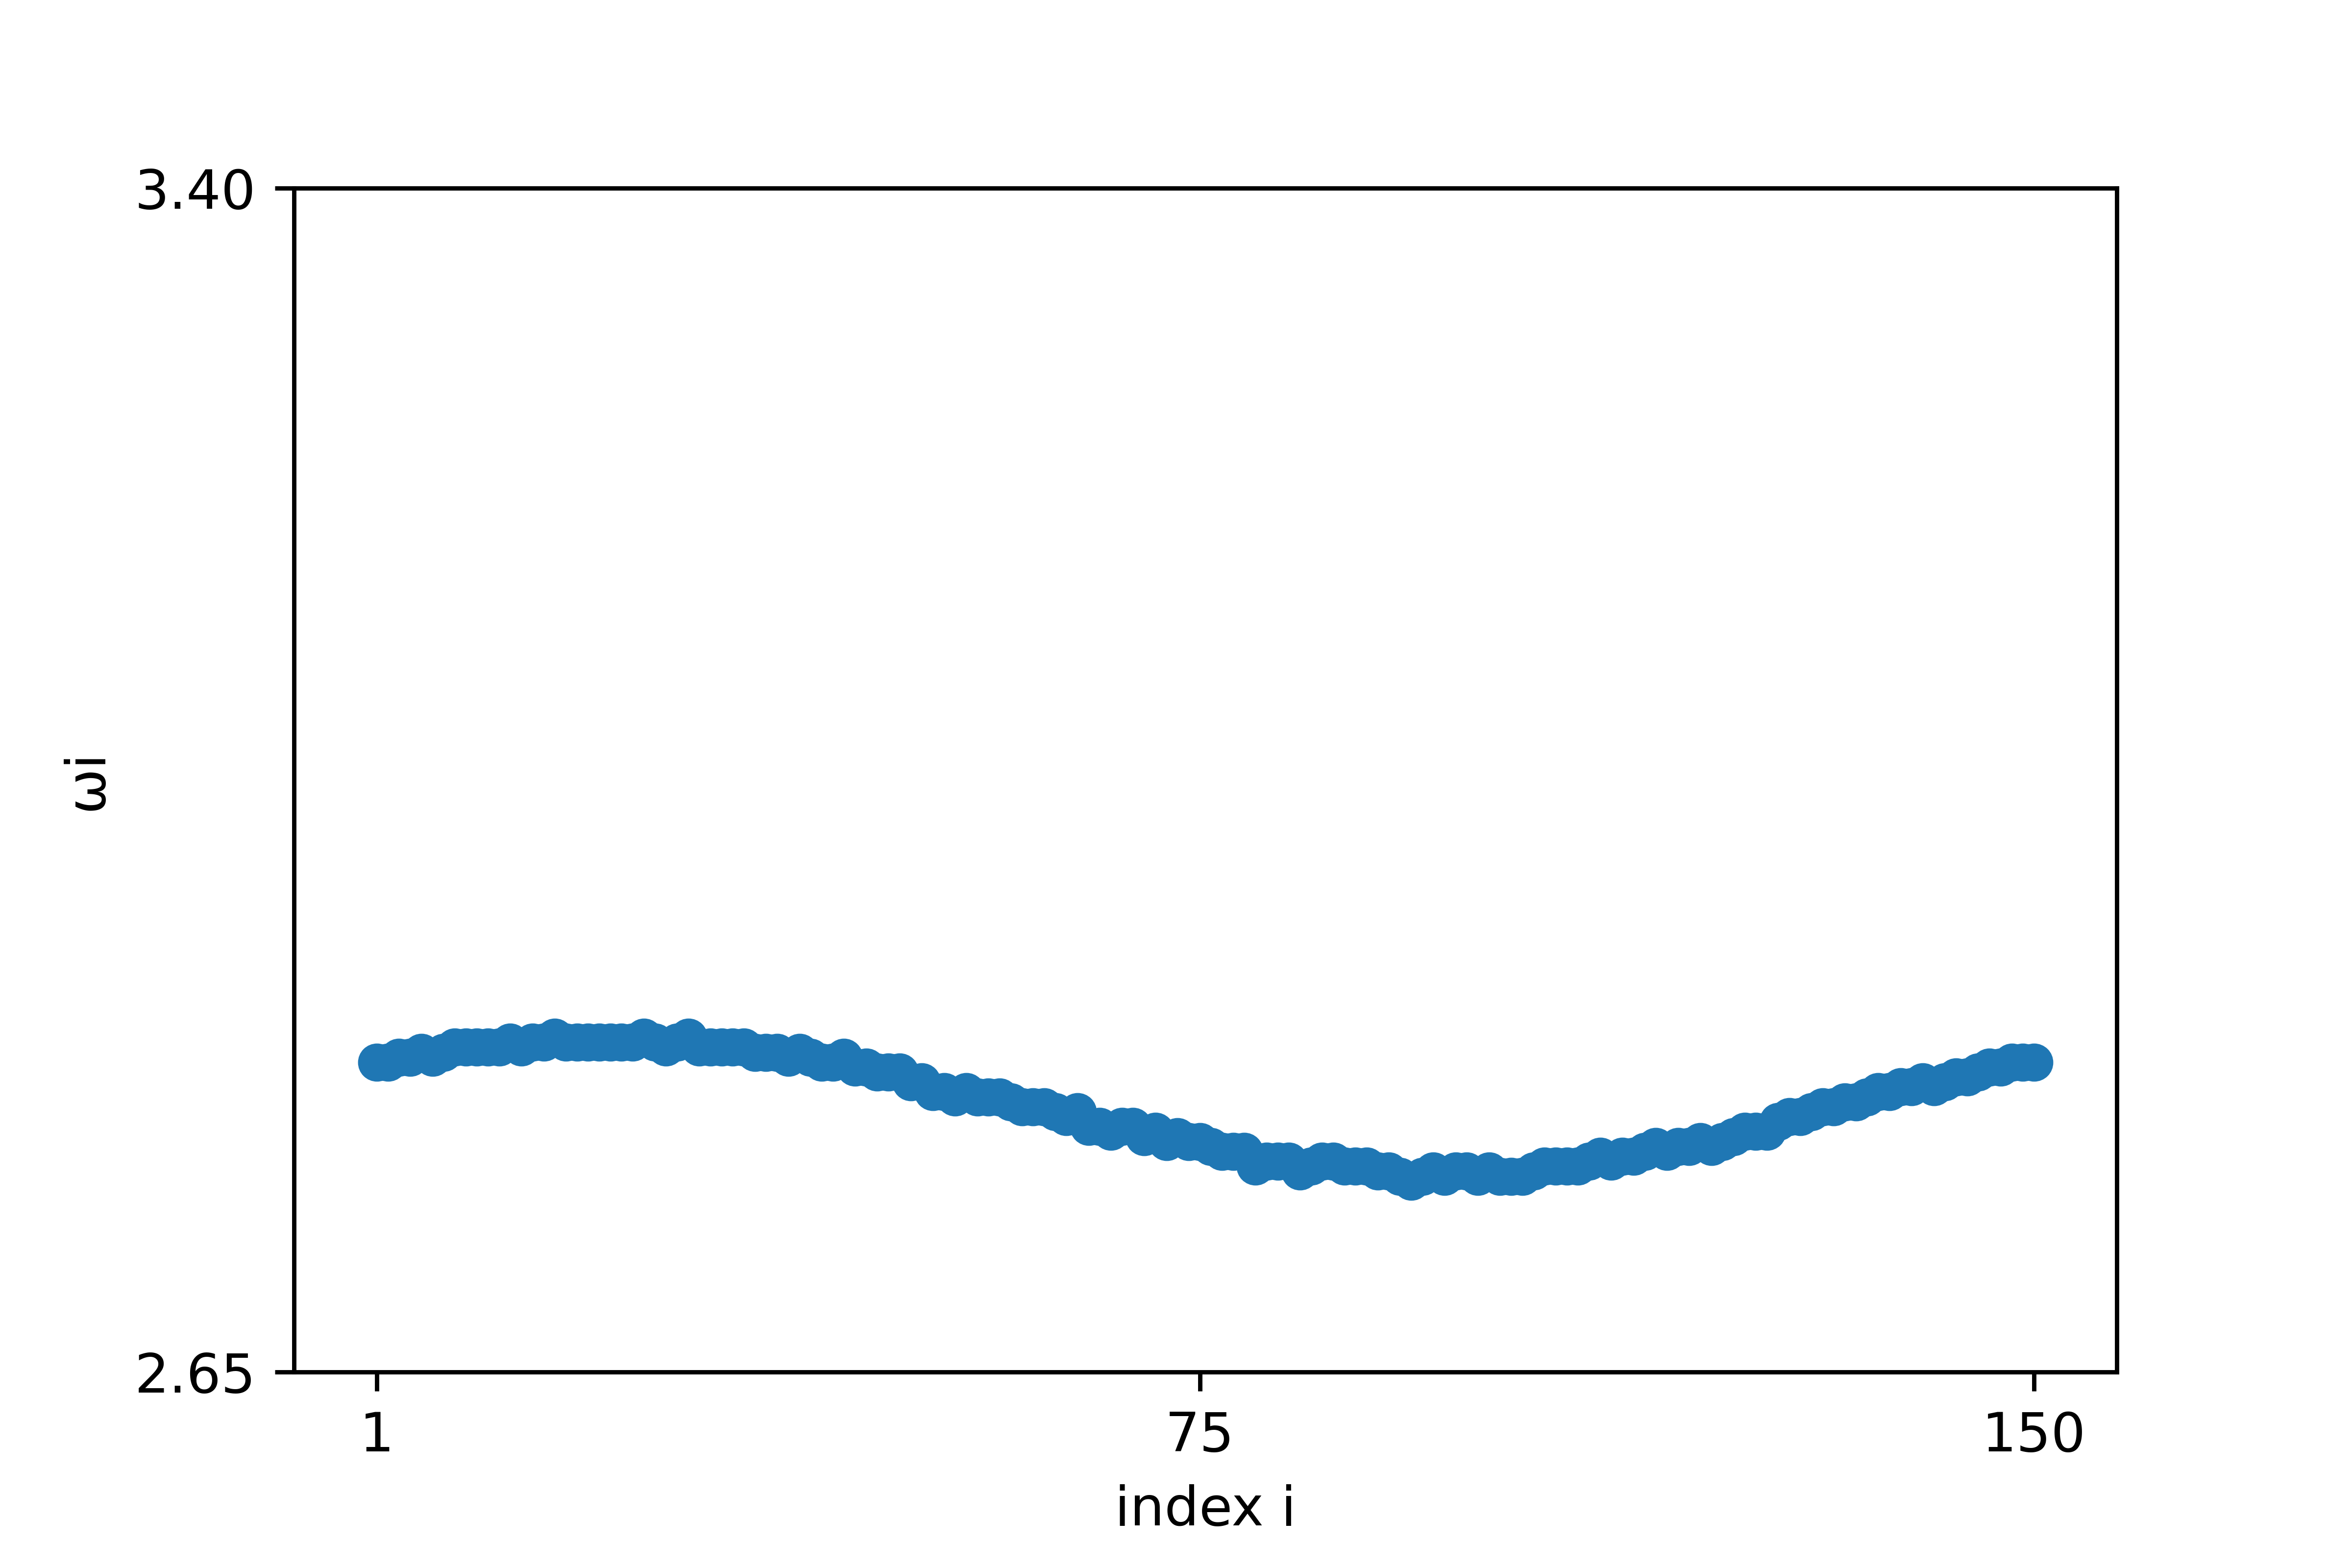
\includegraphics[width=1\linewidth]{w_lambda=0.99_t=2000.png}  
  \caption{$\lambda=0.99$}
\end{subfigure}
\hfill
\begin{subfigure}{.32\textwidth}
  \centering
  % include first image
  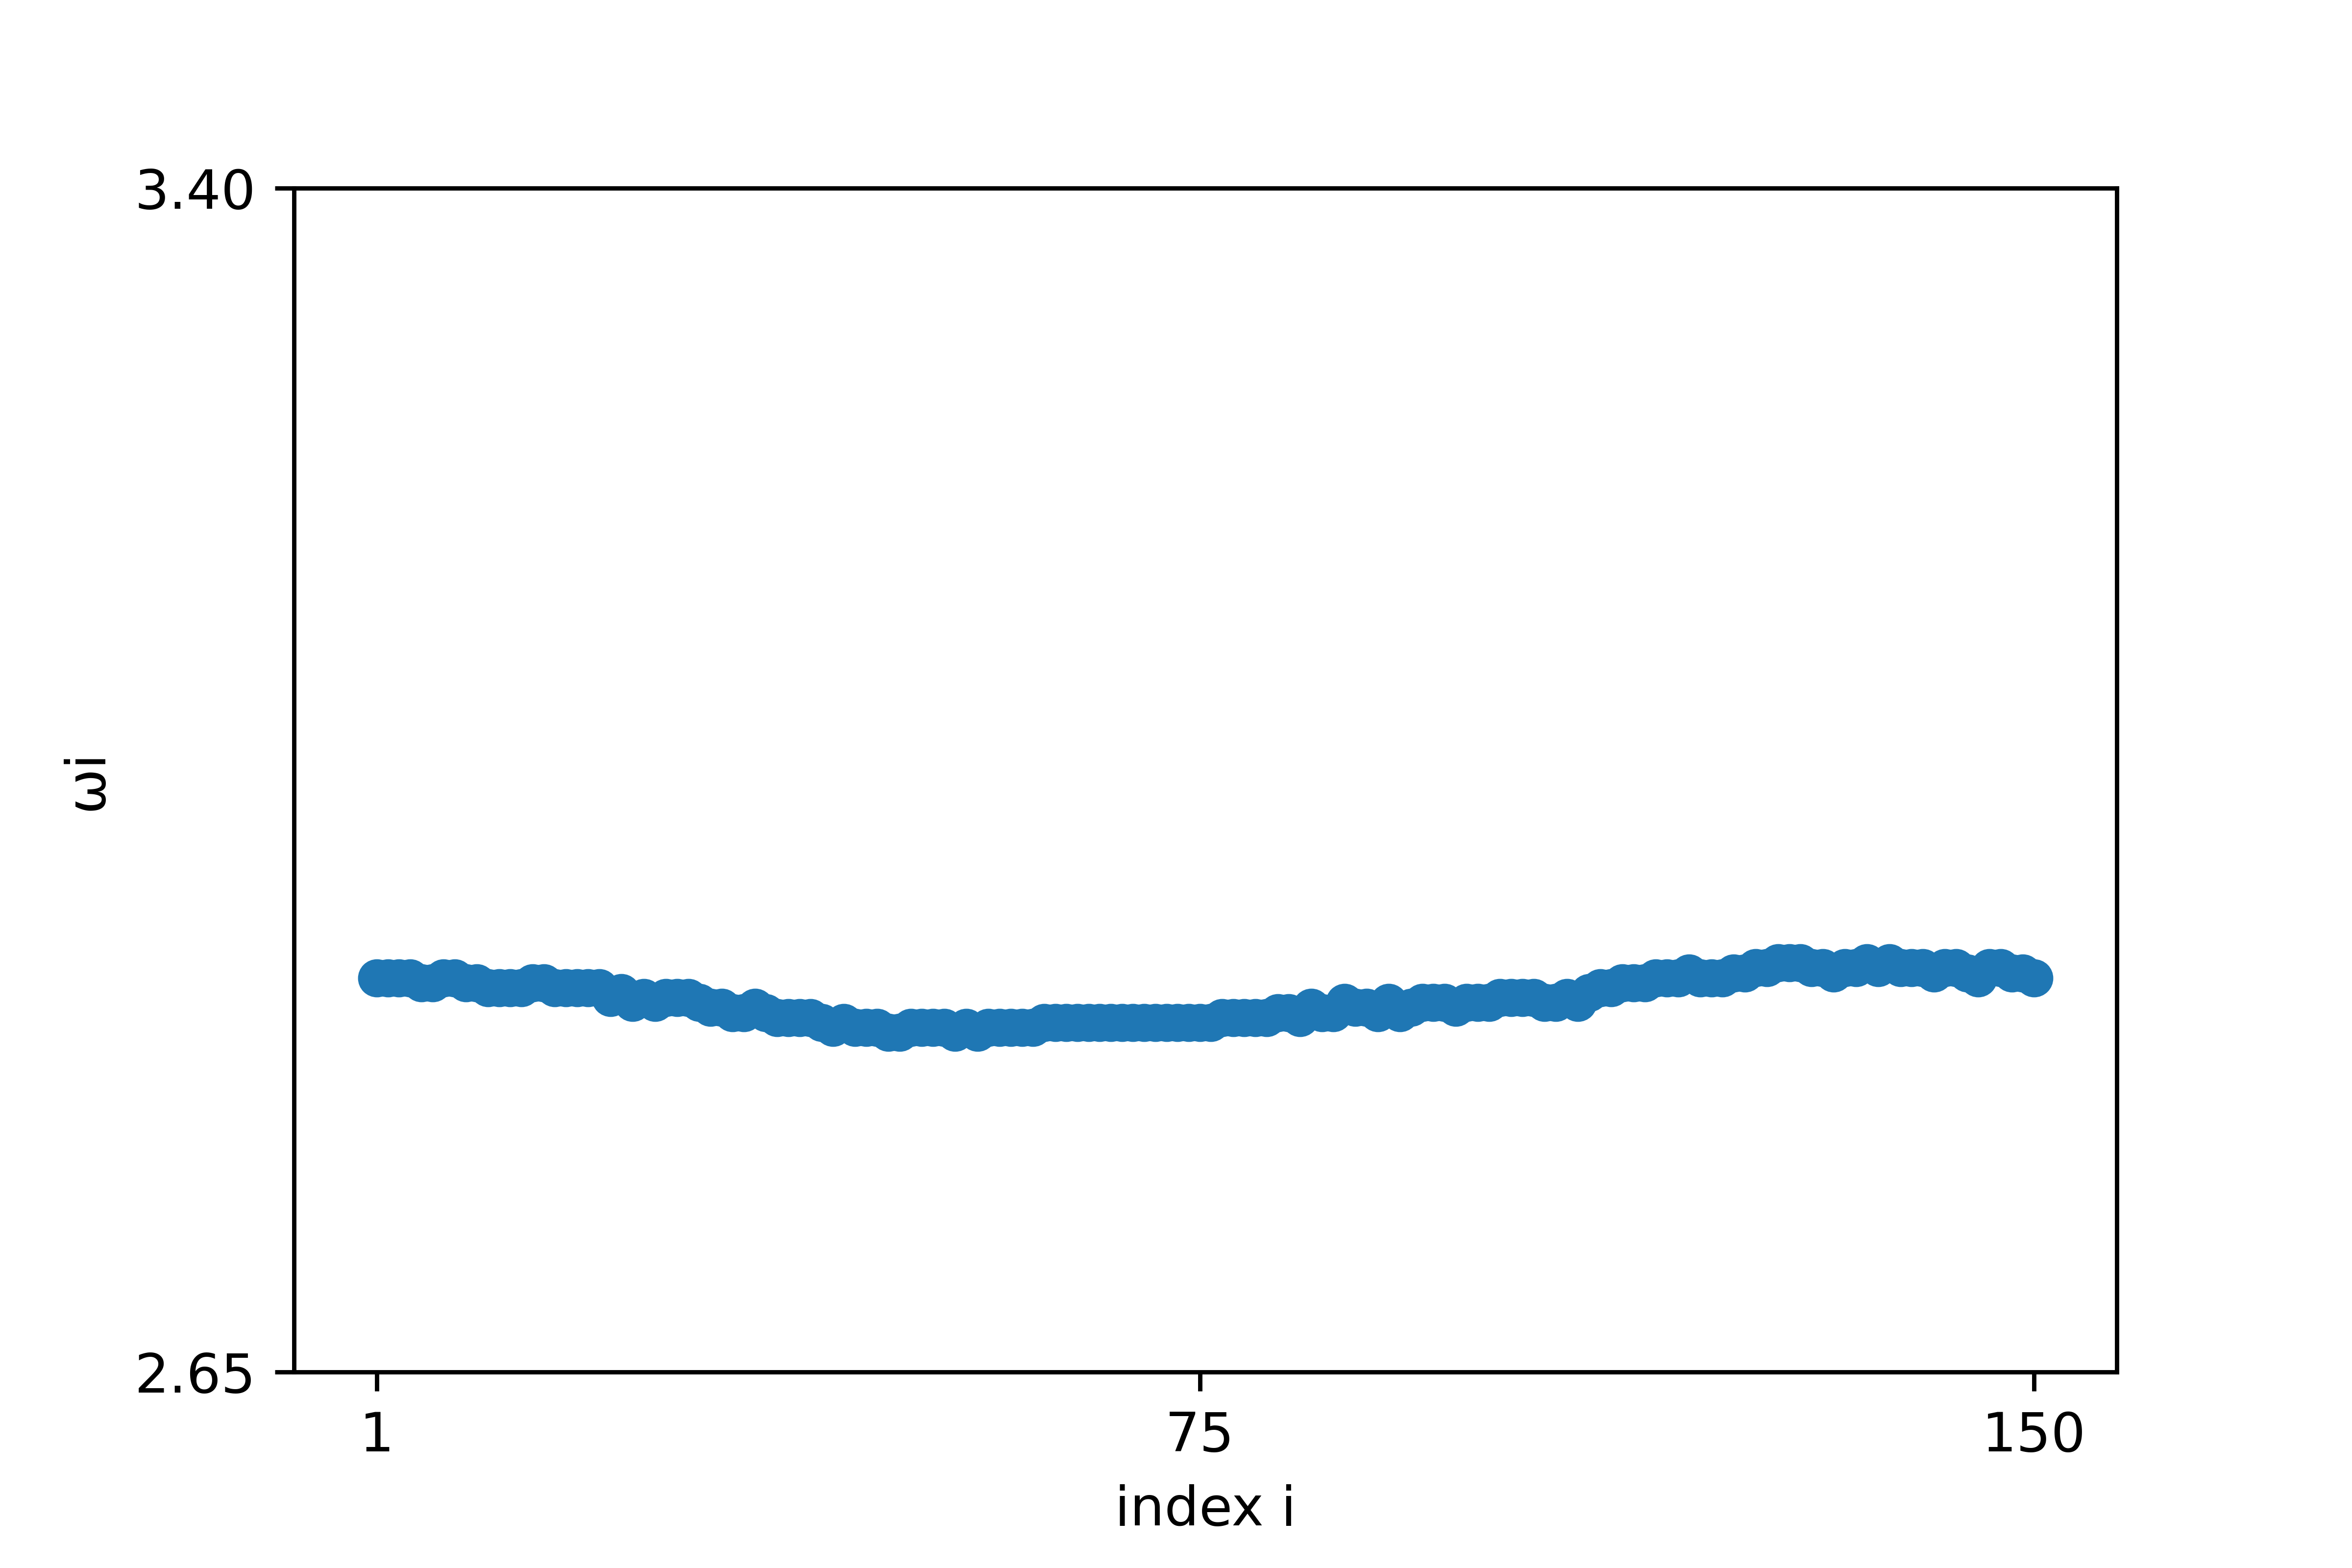
\includegraphics[width=1\linewidth]{w_lambda=0.98_t=2000}  
  \caption{$\lambda=0.98$}
\end{subfigure}
\begin{subfigure}{.32\textwidth}
  \centering
  % include first image
  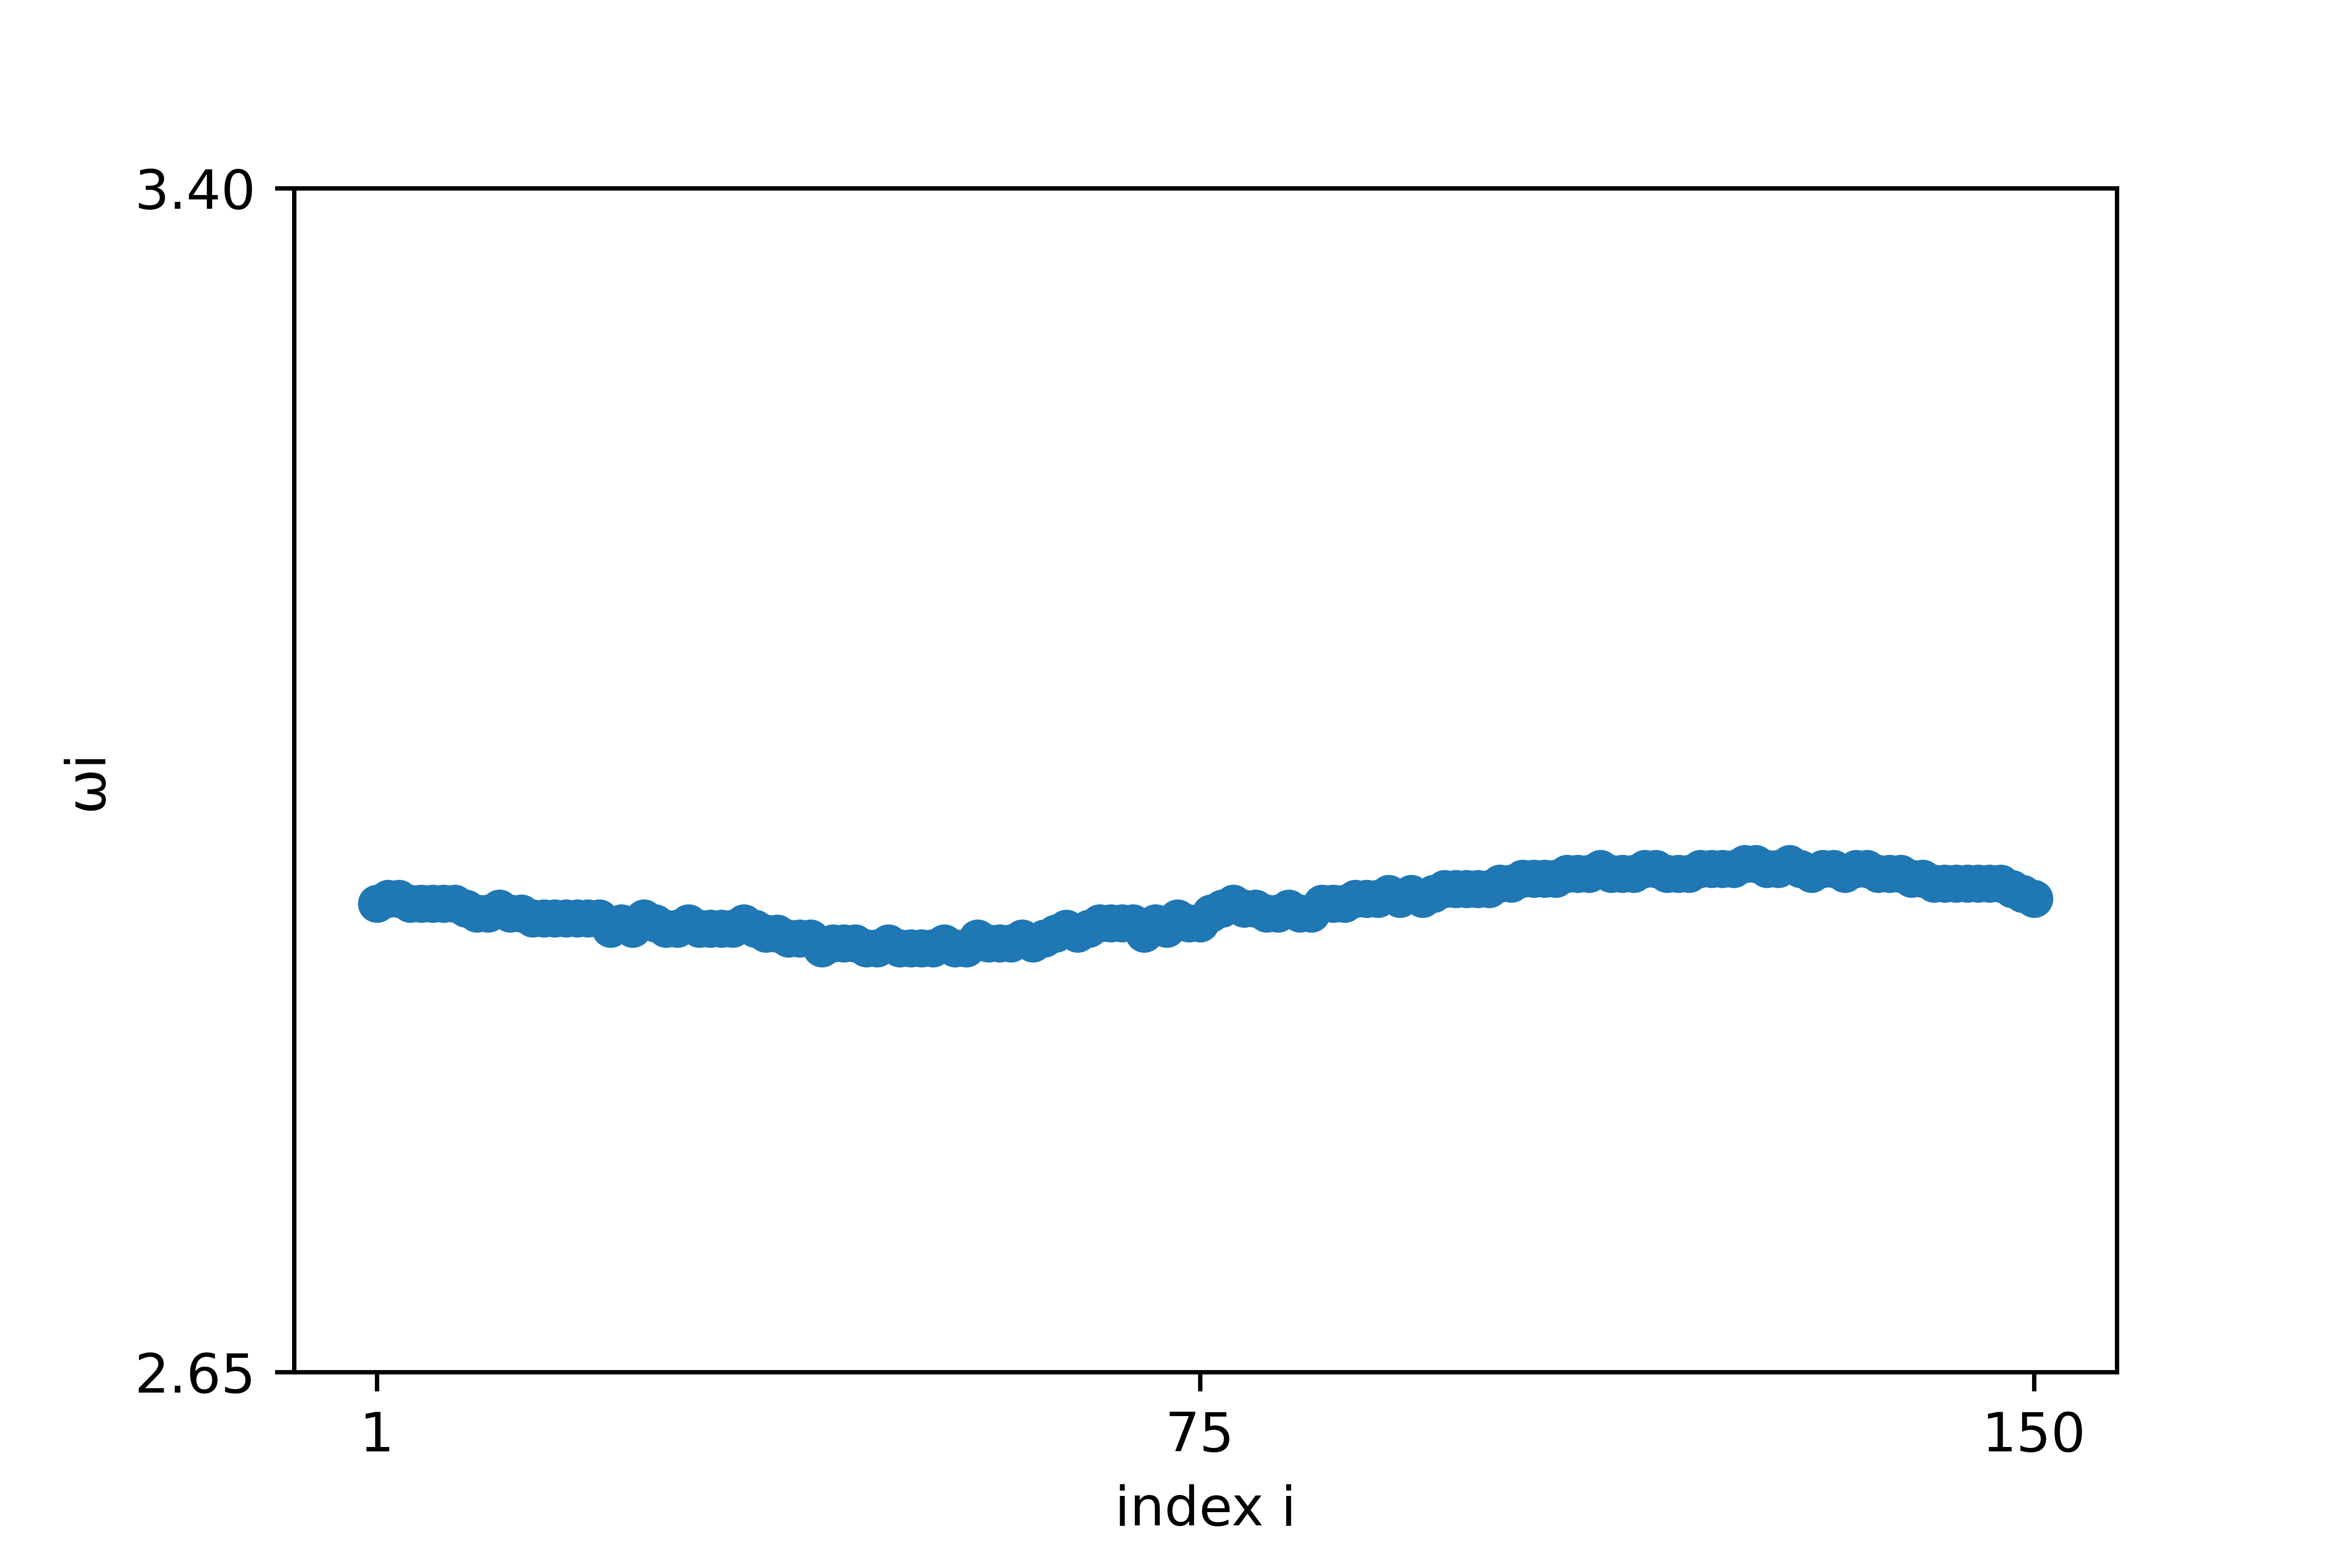
\includegraphics[width=1\linewidth]{w_lambda=0.97_t=2000.png}  
  \caption{$\lambda=0.97$}
\end{subfigure}
\hfill
\begin{subfigure}{.32\textwidth}
  \centering
  % include first image
  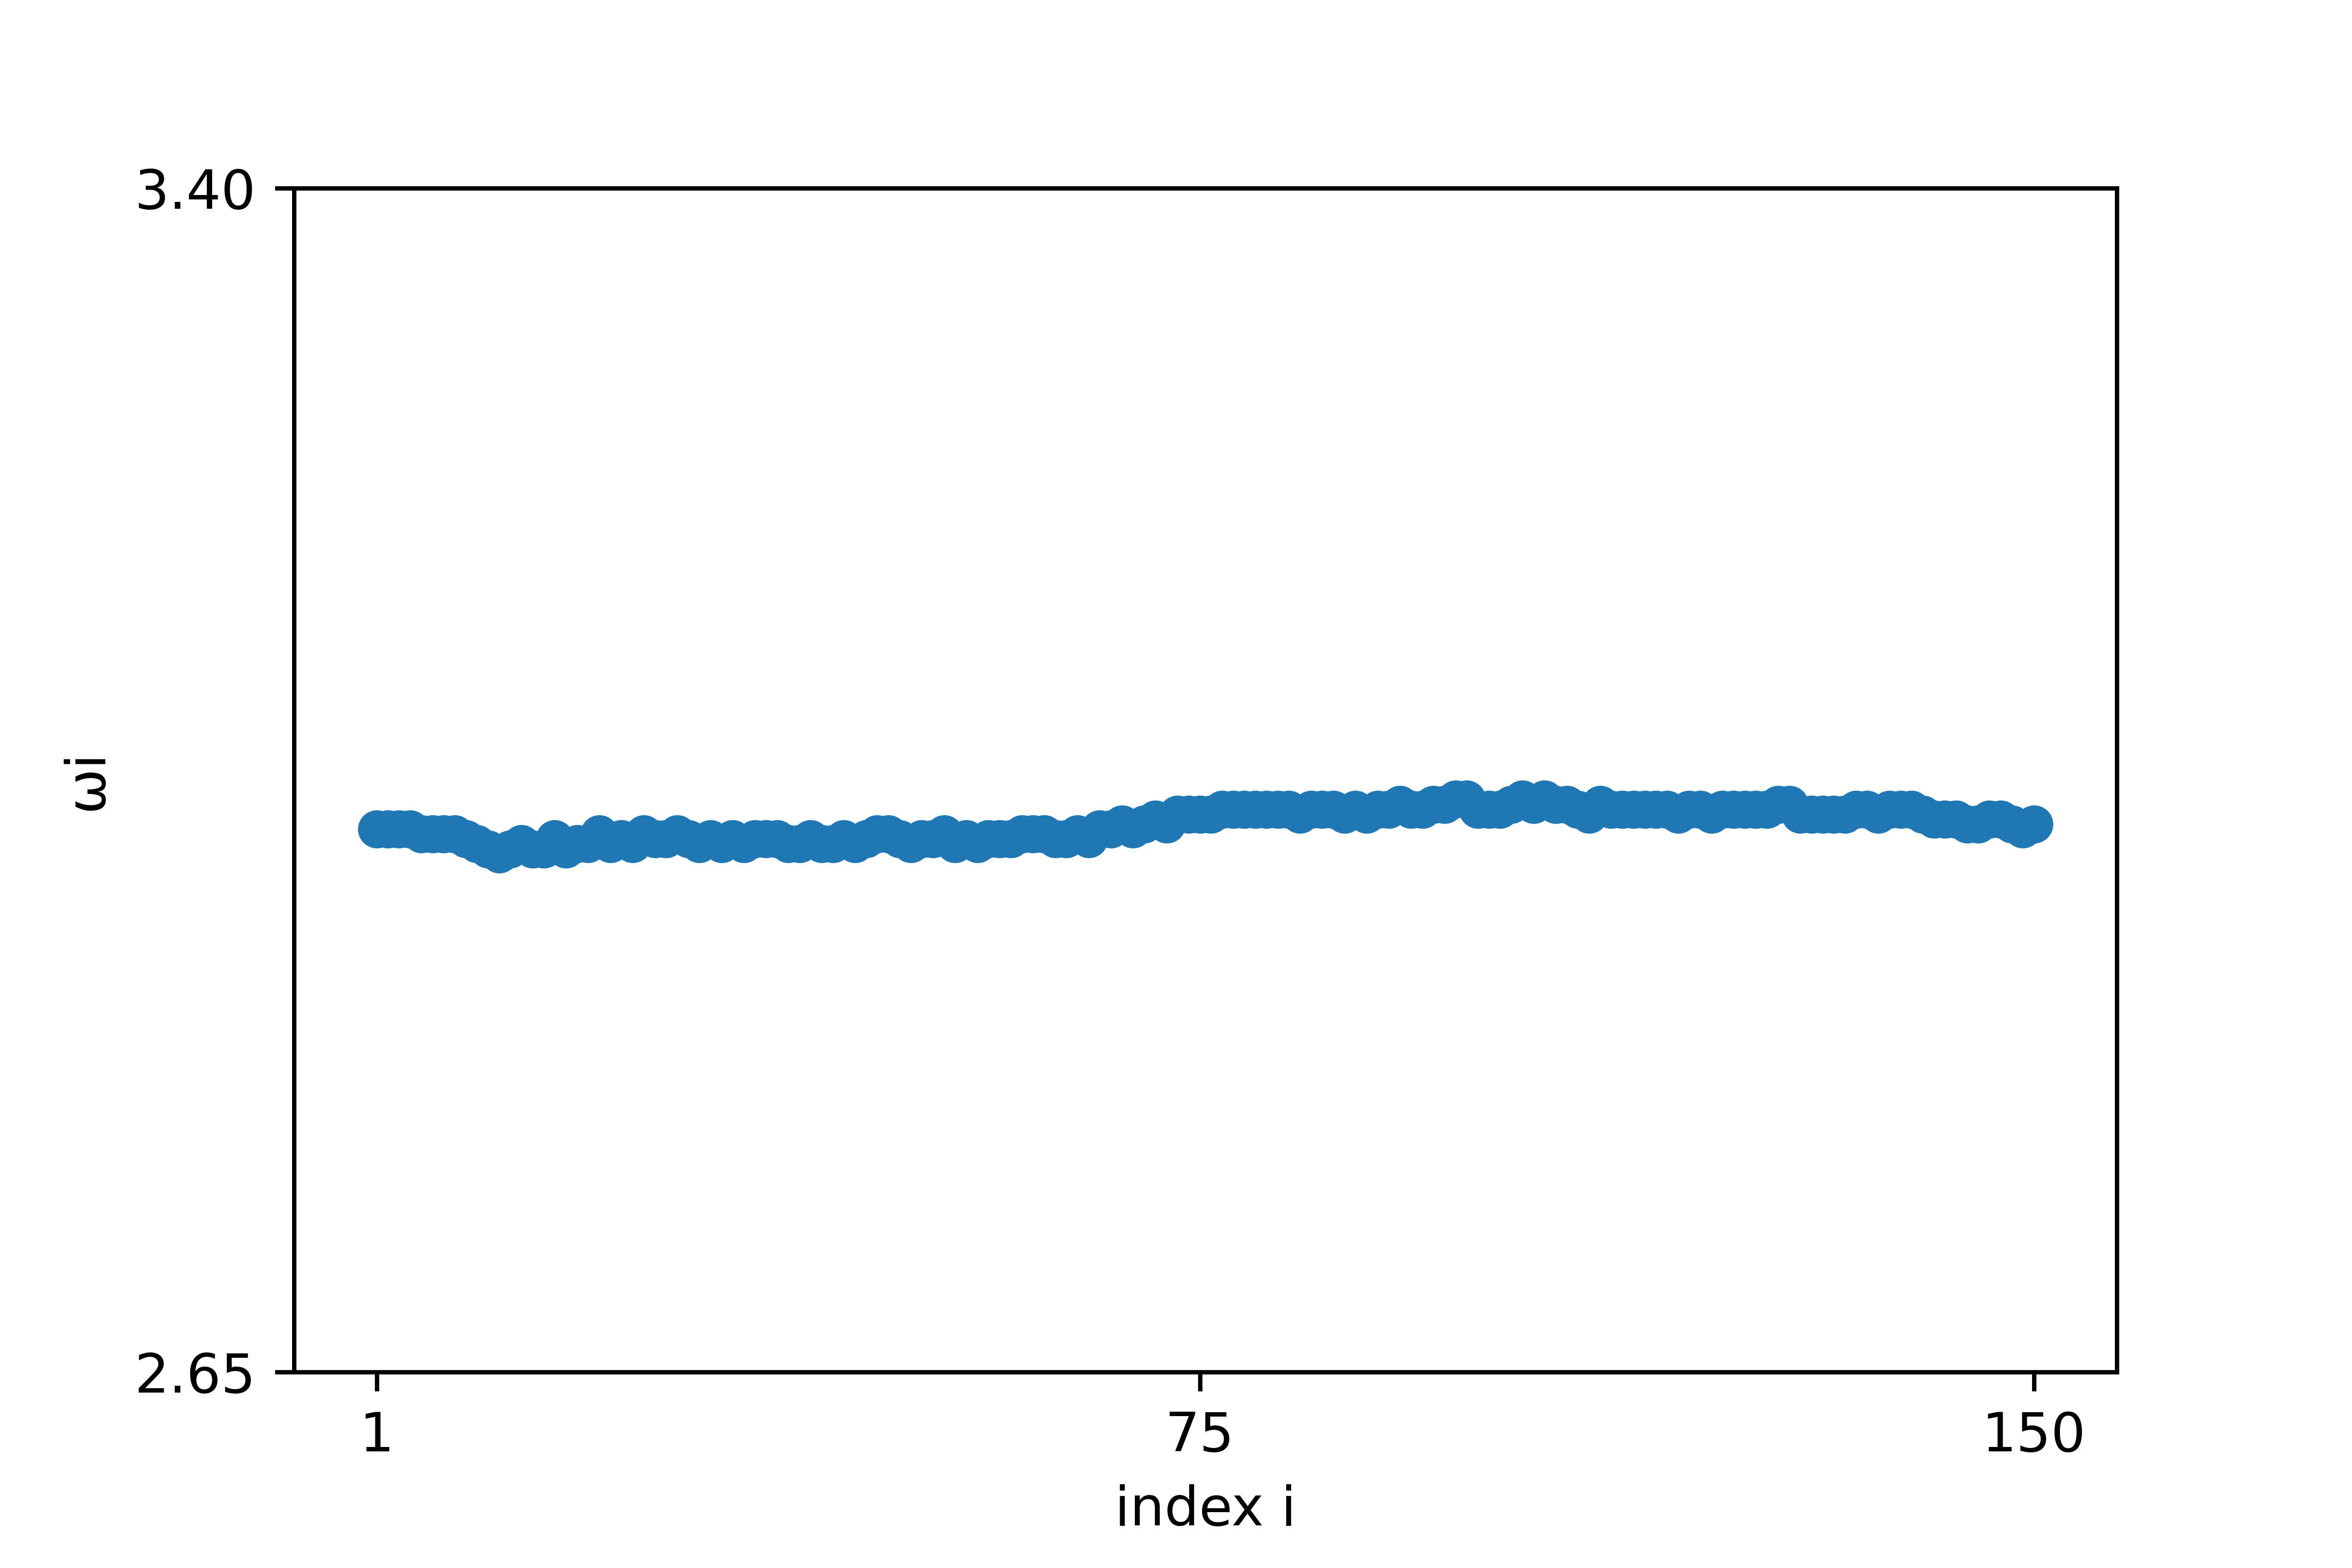
\includegraphics[width=1\linewidth]{w_lambda=0.96_t=2000.png}  
  \caption{$\lambda=0.96$}
\end{subfigure}
\hfill
\begin{subfigure}{.32\textwidth}
  \centering
  % include first image
  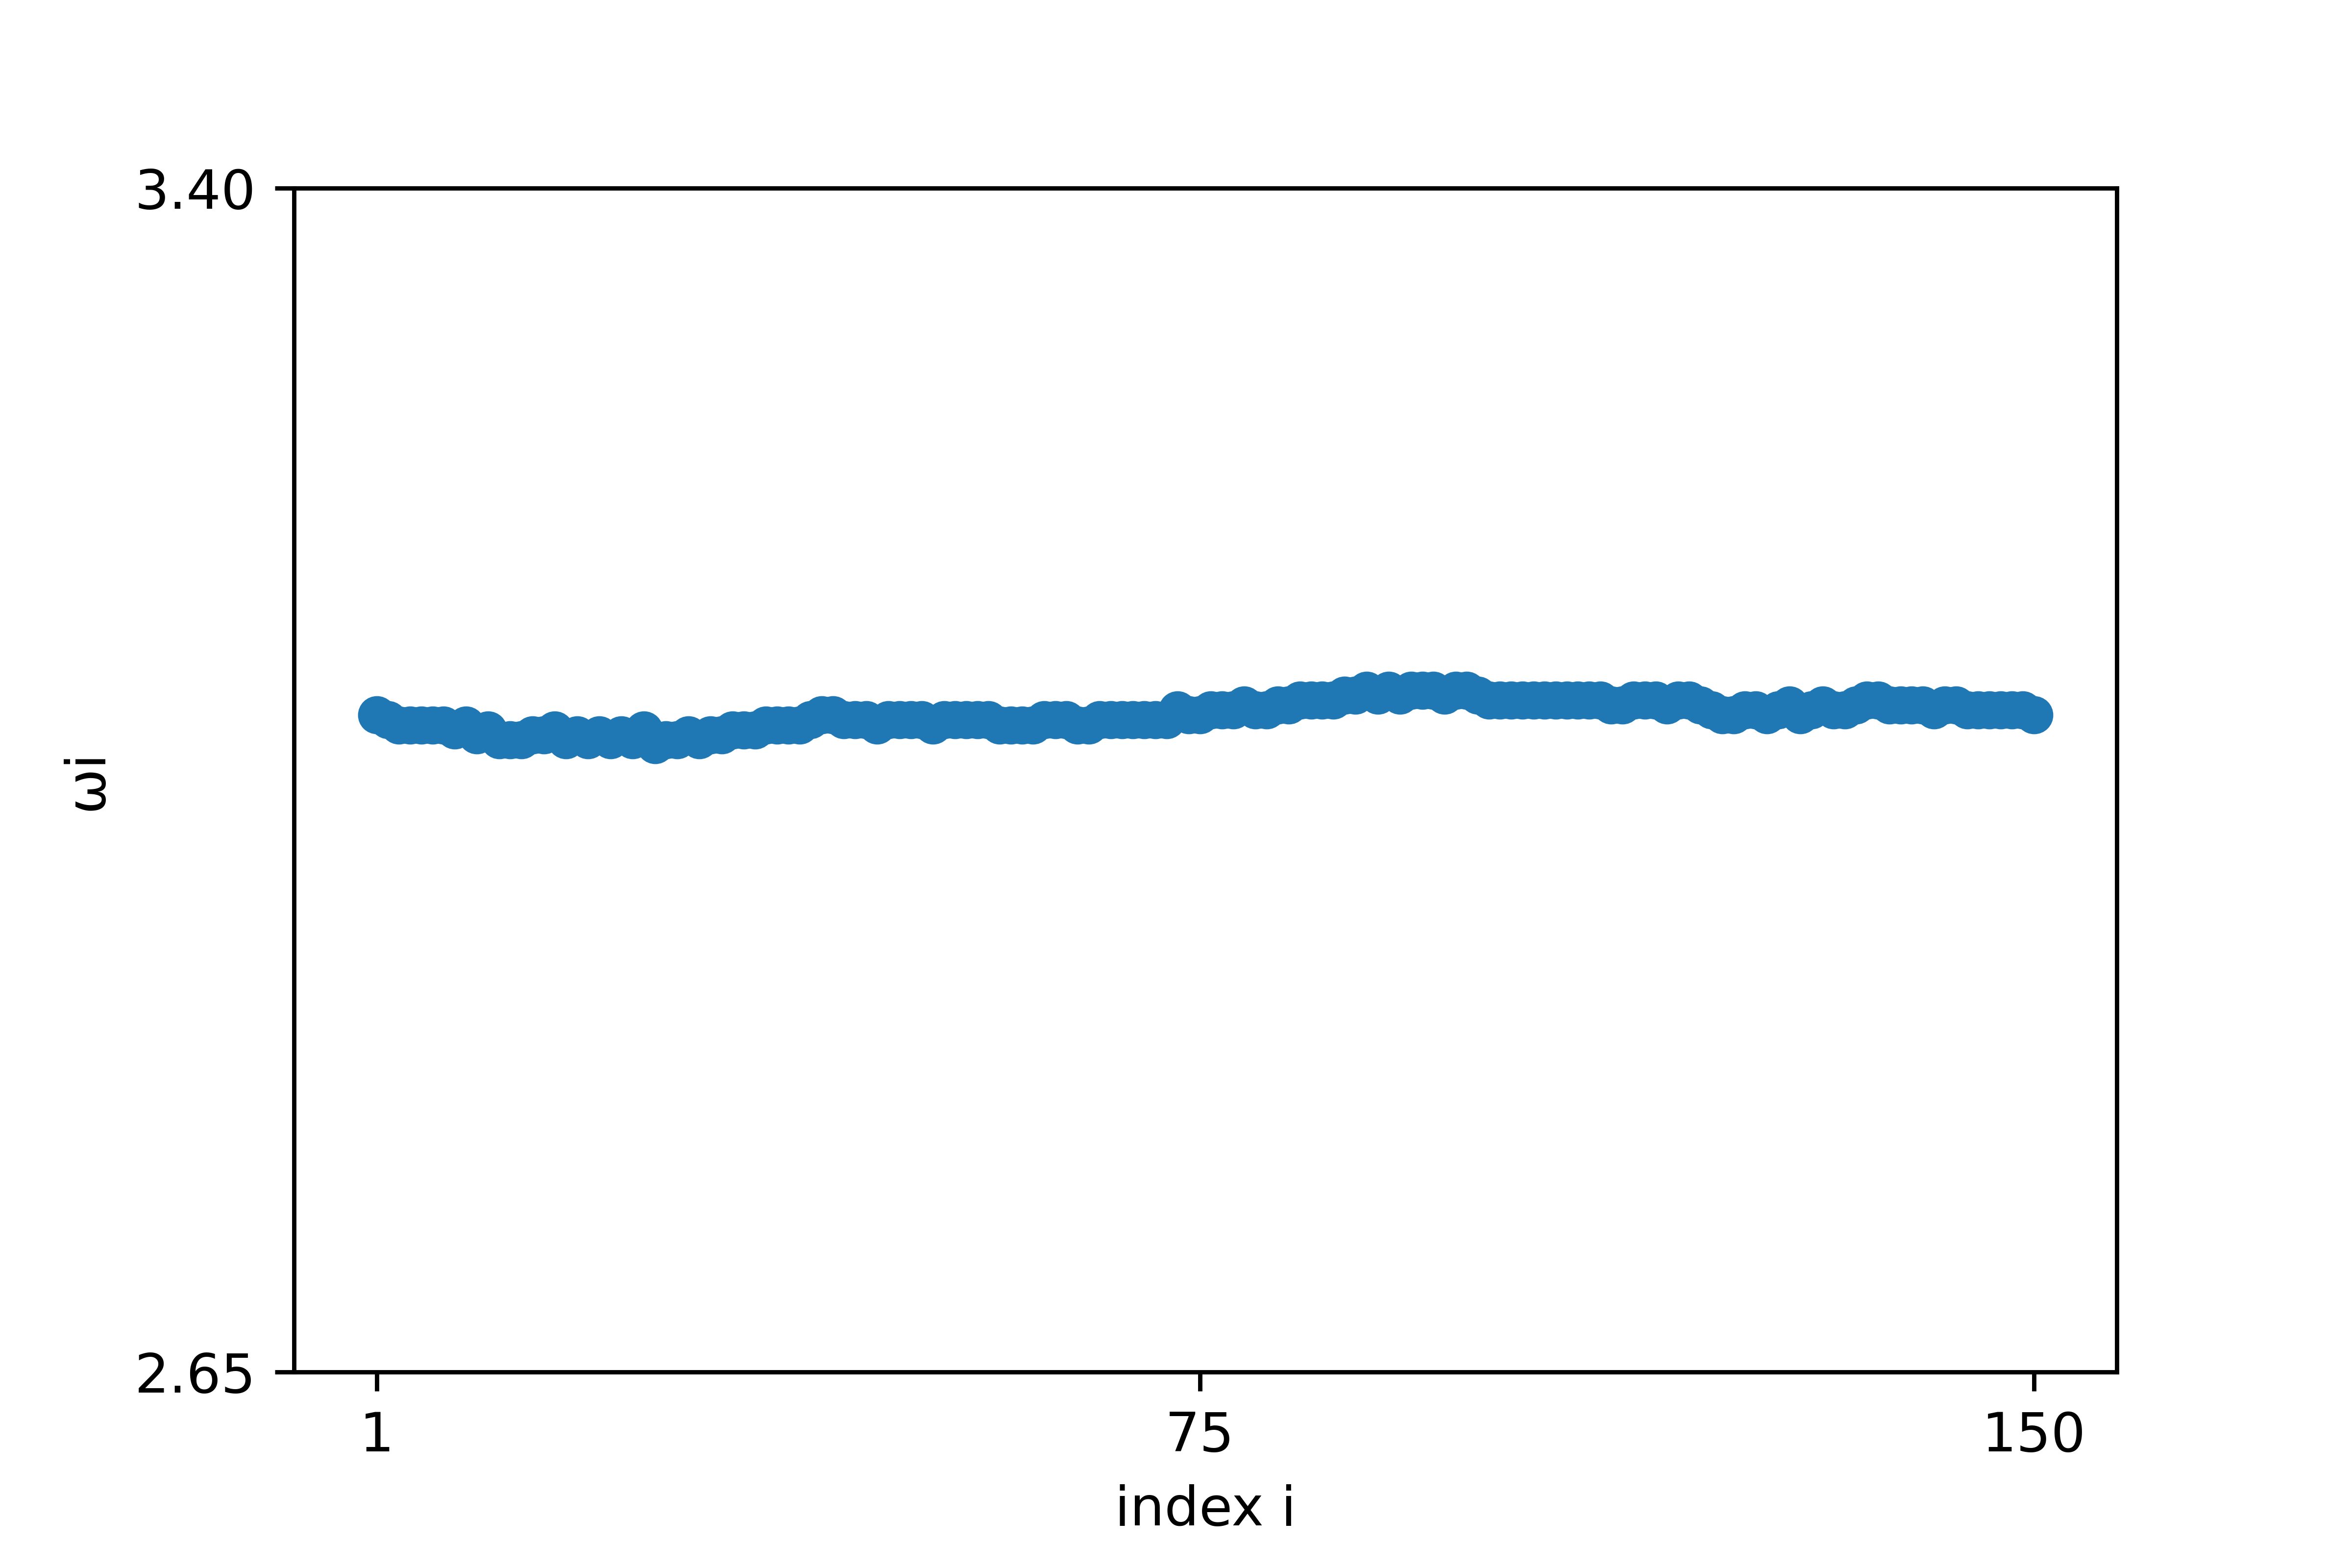
\includegraphics[width=1\linewidth]{w_lambda=0.95_t=2000.png}  
  \caption{$\lambda=0.95$}
\end{subfigure}

\caption{Mean phase-velocity profiles $\omega_i$ at $t=2000$ time units, for $N=150$, $r=0.4$ and $\sigma = 0.7$ and for various values of $\lambda$.}
\label{uivslmd2}
\end{figure}
\end{frame}


\section{Conclusions}
\begin{frame}{Conclusions} \pause
\begin{itemize}
\item chimera states highly dependent on the coupling strength and the coupling range \pause
\item observed chimeras for networks of around $N=100$ neurons \pause
\item when coupling strength is doubled, the single chimera becomes a double chimera \pause
\item high dependence on initial conditions \pause
\item future work: refractory period
\end{itemize}
\end{frame}

\begin{frame}{References}
\begin{small}
\begin{thebibliography}{30}

\bibitem{kuramoto}
Y. Kuramoto and D. Battogtokh. Coexistence of coherence and incoherence in nonlocally coupled phase oscillators. Nonlin. Phen. in Complex Sys., 5:380-385, 2002.

\bibitem{stro}
D. M. Abrams, S. H. Strogatz. Chimera states for coupled oscillators. Phys. Rev. Lett., 93:174102, 2004.

\bibitem{tsigkrimulti}
N. D. Tsigkri-DeSmedt, J. Hizanidis, P. H{\"o}vel, A. Provata. Multi-chimera states and transitions in the leaky integrate-and-fire model with nonlocal and hierarchical connectivity. Eur. Phys. J. Spec. Top., 225:1149–1164, 2016.

\bibitem{tsigkrimulti2}
N. D. Tsigkri-DeSmedt, J. Hizanidis, P. H{\"o}vel, A. Provata. Multi-chimera states in the leaky integrate-and-fire model. Procedia Computer Sci., 66:13-22, 2015.

\bibitem{tsigkrichim}
N. D. Tsigkri-DeSmedt, J. Hizanidis, E. Sch{\"o}ll, A. Provata. Chimeras in leaky integrate-and-fire neural networks: effects of reflecting connectivities. Eur. Phys. J. B, 90:139, 2017.

\end{thebibliography}
\end{small}
\end{frame}

\begin{frame}{Chimera States in the LIF model}
  \centering
  \huge{Thank you!\\}
  \vspace{1cm}
\Large{\today}
  
\end{frame}

\end{document}


